%! TeX program = xelatex

\documentclass[xetex,aspectratio=169,xcolor,professionalfonts,hyperref]{beamer}
\usepackage[
    style=authoryear,
    backend=biber,
    natbib,
    uniquename=false,
    maxcitenames=2,
    maxbibnames=20,
    sorting=nty]{biblatex}
\addbibresource{refs.bib}
\renewcommand*{\bibfont}{\scriptsize}
\usepackage{anyfontsize}
\usepackage{tabularx}
\usepackage{changepage}
\usetheme{dark18}
\usepackage{stmaryrd}
\usepackage{nicefrac}
\usepackage{graphicx}
\usepackage{stackrel}
\usepackage{booktabs}
\usepackage{xspace}
\usepackage{tikz-dependency}
\usepackage{tkz-graph}
\usepackage{pgfplots}
\usepgfplotslibrary{groupplots}
% emojis!
\makeatletter
\newcommand*\fsize{\dimexpr\f@size pt\relax}
\makeatother
\newcommand*\emoji[2][1]{\includegraphics[width=#1\fsize]{emoji/#2}}
%
%% Generic TiKZ utils!
\usetikzlibrary{calc,backgrounds,arrows,arrows.meta}
\usetikzlibrary{decorations.pathreplacing}
\usetikzlibrary{tikzmark,positioning,patterns}
\usetikzlibrary{bending}
\usetikzlibrary{overlay-beamer-styles}
\pgfdeclarelayer{background}
\pgfdeclarelayer{foreground}
\pgfsetlayers{background,main,foreground}
%
\tikzset{
    visible on/.style={alt={#1{}{invisible}}},
    invisible/.style={opacity=0},
    alt/.code args={<#1>#2#3}{%
      \alt<#1>{\pgfkeysalso{#2}}{\pgfkeysalso{#3}} % \pgfkeysalso doesn't change the path
    },
  }

%% particular stuff?
\newcommand*{\ticksize}{2pt}
\tikzset{axisline/.style={thick,myfg!50!mybg,text=myfg,font=\small}}
\tikzset{axislabel/.style={font=\small}}
\tikzset{point/.style={thick,tMidnight}}


% semantic color definitions
\colorlet{colorArgmax}{tTarmac}
\colorlet{colorSoftmax}{tVividBlue}
\colorlet{colorSparsemax}{tYellow!50}
\colorlet{colorFusedmax}{tPeony!80!mybg}
\colorlet{colorEntmax}{tPeony}


\tikzset{
    tinyarrowl/.style={-{Straight Barb[bend]},thick,bend left=75,tPeony},
    tinyarrowr/.style={-{Straight Barb[bend]},thick,bend right=75,tPeony}}
\newcommand{\miniparse}[1]{%
{\footnotesize%
\begin{tikzpicture}[
    node distance=14pt,
    every node/.style={inner sep=0,outer sep=1pt},
    ]
\node[tPeony] (a) at (0, 0) {\textbullet};
\node[tPeony,right of=a] (b) {\textbullet};
\node[tPeony,right of=b] (c) {\textbullet};
\foreach \i/\j/\r/\o in {#1}{
\path (\i.north) edge[tinyarrow\r,opacity=\o] (\j.north);
}\end{tikzpicture}}}

% Tikz pic: draw a cog
\tikzset{cog/.pic={code={
    \draw[myfg,thick,fill=tTarmac!90]
  (0:2)
  \foreach \i [evaluate=\i as \n using {(\i-1)*360/18}] in {1,...,18}{%
    arc (\n:\n+10:2) {[rounded corners=1.5pt] -- (\n+10+2:2.4)
    arc (\n+10+2:\n+360/18-2:2.4)} --  (\n+360/18:2)
  };
  \draw[myfg,thick,fill=mybg] (0,0) circle[radius=.5];
}}}
%
%
% Tikz: draw an envelope
\newsavebox\envelope
\savebox{\envelope}{

\newlength\mylen
\setlength\mylen{2cm}
\begin{tikzpicture}[scale=.65]

\coordinate (A) at (0,0);
\coordinate (B) at (1.41\mylen,-\mylen);
\clip
  ([xshift=-0.5\pgflinewidth,yshift=0.5\pgflinewidth]A) --
  ([xshift=0.5\pgflinewidth,yshift=0.5\pgflinewidth]A-|B) --
  ([xshift=0.5\pgflinewidth,yshift=-0.5\pgflinewidth]B) --
  ([xshift=-0.5\pgflinewidth,yshift=-0.5\pgflinewidth]B-|A) --
  ([xshift=-0.5\pgflinewidth,yshift=0.5\pgflinewidth]A);
\draw[mybg,fill=tTarmac,line cap=rect]
  (A) -- (A-|B) -- (B) -- (B-|A) -- (A);
\draw[mybg]
  (B-|A) -- (0.705\mylen,-.3\mylen) -- (B);
\draw[mybg,fill=tTarmac!90,rounded corners=15pt]
  (A) -- (0.705\mylen,-0.6\mylen) -- (A-|B);
\node[anchor=north]
  at ($ (A)!0.5!(B|-A) $ ) {\parbox{\mylen}{}};
\draw[mybg] (A) -- (B|-A);
\end{tikzpicture}
}
%
% output
\newsavebox\sentoutput
\savebox{\sentoutput}{%
    \begin{tikzpicture}[scale=.75,text=myfg]
 \draw[rounded corners,tTarmac!60,very thick] (-.5, -.5) rectangle (.5, 2.5) {};

 \node[label={[label distance=.25cm]0:positive}] (pos) at (0, 2) {};
 \node[label={[label distance=.25cm]0:neutral}] (neu) at (0, 1) {};
 \node[label={[label distance=.25cm]0:negative}] (neg) at (0, 0) {};

 \draw[fill=tNavy!80!myfg] (pos) circle[radius=9pt];
 \draw[fill=tNavy!20!myfg] (neu) circle[radius=9pt];
 \draw[fill=tNavy!20!myfg] (neg) circle[radius=9pt];
 \end{tikzpicture}
 }
%
% cartoon structure
\newcommand{\cartoon}[2][1]{%
\begin{tikzpicture}%
\node[draw=none, minimum size=#1*1cm, regular polygon, regular polygon sides=5] (p) {};
%
\foreach \i/\j in {#2}%
{
    \draw[tPeony, ultra thick] (p.corner \i) -- (p.corner \j);
}
%
\foreach \i in {1, ..., 5}%
{
    \draw[myfg,fill=mybg,very thick] (p.corner \i) circle[radius=#1*5pt];
}
\end{tikzpicture}}
\newcommand{\cartoonDense}[1][1]{%
\begin{tikzpicture}%
\node[draw=none, minimum size=#1*1cm, regular polygon, regular polygon sides=5] (p) {};
%
\draw[tPeony, ultra thick, opacity=.8] (p.corner 1) -- (p.corner 2);
\draw[tPeony, ultra thick, opacity=.5] (p.corner 1) -- (p.corner 3);
\draw[tPeony, ultra thick, opacity=.7] (p.corner 1) -- (p.corner 4);
\draw[tPeony, ultra thick, opacity=.4] (p.corner 1) -- (p.corner 5);
\draw[tPeony, ultra thick, opacity=.6] (p.corner 2) -- (p.corner 3);
\draw[tPeony, ultra thick, opacity=.3] (p.corner 2) -- (p.corner 4);
\draw[tPeony, ultra thick, opacity=.9] (p.corner 2) -- (p.corner 5);
\draw[tPeony, ultra thick, opacity=.2] (p.corner 3) -- (p.corner 4);
\draw[tPeony, ultra thick, opacity=.6] (p.corner 3) -- (p.corner 5);
\draw[tPeony, ultra thick, opacity=.4] (p.corner 4) -- (p.corner 5);
%
\foreach \i in {1, ..., 5}%
{
    \draw[myfg,fill=mybg,very thick] (p.corner \i) circle[radius=#1*5pt];
}
\end{tikzpicture}}
\newcommand{\cartoonSparse}[1][1]{%
\begin{tikzpicture}%
\node[draw=none, minimum size=#1*1cm, regular polygon, regular polygon sides=5] (p) {};
%
\draw[tPeony, ultra thick, opacity=1] (p.corner 1) -- (p.corner 4);
\draw[tPeony, ultra thick, opacity=.5] (p.corner 2) -- (p.corner 5);
\draw[tPeony, ultra thick, opacity=.5] (p.corner 1) -- (p.corner 5);
%
\foreach \i in {1, ..., 5}%
{
    \draw[myfg,fill=mybg,very thick] (p.corner \i) circle[radius=#1*5pt];
}
\end{tikzpicture}}
%
\newcommand{\setupsimplexbary}[1][3.3]{%
\coordinate (L1) at (0:0);
\coordinate (L2) at (0:#1);
\coordinate (L3) at (60:#1);

\node[label=east:{\small$\triangle$}] at (L2) {};

\fill[tYellow,opacity=.15]  (L1) -- (L2) -- (L3) -- cycle;
\draw[very thick,tYellow] (L1) -- (L2) -- (L3) -- cycle;

\draw[tYellow,fill] (L1) circle[radius=3pt];
\draw[tYellow,fill] (L2) circle[radius=3pt];
\draw[tYellow,fill] (L3) circle[radius=3pt];
}

\newcommand{\drawcs}{%
\node[anchor=south] at (0, \vecheight*4) {$c_1$};
\node[anchor=south] at (0, \vecheight*3) {$c_2$};
\node[anchor=south] at (0, \vecheight*1.5) {$\cdots$};
\node[anchor=south] at (0, \vecheight*0) {$c_N$};}

\newcommand{\drawscores}{%
\node[anchor=south] at (-1-.5*\vecwidth, \vecheight*5+.1) {$\s$};
\draw[elem,fill=vecfg!60!vecbg] (-1-\vecwidth, \vecheight*4) rectangle (-1, \vecheight*5);
\draw[elem,fill=vecfg!85!vecbg] (-1-\vecwidth, \vecheight*3) rectangle (-1, \vecheight*4);
\draw[elem,fill=vecfg!60!vecbg] (-1-\vecwidth, \vecheight*2) rectangle (-1, \vecheight*3);
\draw[elem,fill=vecfg!75!vecbg] (-1-\vecwidth, \vecheight*1) rectangle (-1, \vecheight*2);
\draw[elem,fill=vecfg!50!vecbg] (-1-\vecwidth, \vecheight*0) rectangle (-1, \vecheight*1);
}

\newcommand{\drawargmax}{%
\node[anchor=south] at (1+.5*\vecwidth, \vecheight*5+.1) {$\p$};
\draw[elem,fill=vecfg! 0!vecbg]  (1, \vecheight*4) rectangle (1+\vecwidth, \vecheight*5);
\draw[elem,fill=vecfg!70!vecbg]  (1, \vecheight*3) rectangle (1+\vecwidth, \vecheight*4);
\draw[elem,fill=vecfg! 0!vecbg]  (1, \vecheight*2) rectangle (1+\vecwidth, \vecheight*3);
\draw[elem,fill=vecfg! 0!vecbg]  (1, \vecheight*1) rectangle (1+\vecwidth, \vecheight*2);
\draw[elem,fill=vecfg! 0!vecbg]  (1, \vecheight*0) rectangle (1+\vecwidth, \vecheight*1);
}
\newcommand{\drawsoftmax}{%
\node[anchor=south] at (1+.5*\vecwidth, \vecheight*5+.1) {$\p$};
\draw[elem,fill=vecfg!30!vecbg]  (1, \vecheight*4) rectangle (1+\vecwidth, \vecheight*5);
\draw[elem,fill=vecfg!50!vecbg]  (1, \vecheight*3) rectangle (1+\vecwidth, \vecheight*4);
\draw[elem,fill=vecfg!35!vecbg]  (1, \vecheight*2) rectangle (1+\vecwidth, \vecheight*3);
\draw[elem,fill=vecfg!25!vecbg]  (1, \vecheight*1) rectangle (1+\vecwidth, \vecheight*2);
\draw[elem,fill=vecfg!15!vecbg]  (1, \vecheight*0) rectangle (1+\vecwidth, \vecheight*1);
}


% math and notation
\newcommand*\bs[1]{\boldsymbol{#1}}
\newcommand\defeq{{\,\raisebox{1pt}{$:$}=}\,}
\newcommand\p{\bs{p}}
\newcommand\xx{z}
\newcommand\x{\bs{\xx}}
\newcommand\s{\x}
\renewcommand\ss{\xx}
\newcommand\mg{\bs{\mu}}
\newcommand\pr{\bs{\eta}}
\newcommand\Mp{\mathcal{M}}
\newcommand\parp{\bs{\pi}}
\newcommand\clfp{\bs{\phi}}
\DeclareMathOperator*{\argmax}{arg\,max}
\DeclareMathOperator*{\argmin}{arg\,min}
\DeclareMathOperator{\HH}{H}
\DeclareMathOperator{\mapo}{\bs{\pi}_{\Omega}}
\DeclareMathOperator{\diag}{diag}
\DeclareMathOperator{\ident}{Id}
\DeclareMathOperator{\dom}{dom}
\DeclareMathOperator{\conv}{conv}
\newcommand\reals{\mathbb{R}}

\newcommand{\pfrac}[2]{\frac{\partial #1}{\partial #2}}
\newcommand{\langp}[2]{\textsc{#1}$\shortrightarrow$\textsc{#2}}
\newcommand{\langpb}[2]{\textsc{#1}$\leftrightarrow$\textsc{#2}}
\newcommand*\entmaxtext{entmax\xspace}
\DeclareMathOperator*{\entmax}{\mathsf{\entmaxtext}}
\newcommand*\aentmax[1][\alpha]{\mathop{\mathsf{#1}\textnormal{-}\mathsf{\entmaxtext}}}
\DeclareMathOperator*{\softmaxlight}{\mathsf{softmax}}

% smaller and gray citation
\let\realcitep\citep
\renewcommand*{\citep}[1]{{\color{mygr}\scriptsize\realcitep{#1}}}
\newcommand*{\citeparg}[2]{{\color{mygr}\scriptsize\parencite[][#2]{#1}}}

\usepackage{etoolbox}
\usepackage{fp}
\makeatletter
\newcounter{ROWcellindex@}
\newtoggle{@doneROWreads}
\newcommand\setstackEOL[1]{%
  \ifstrempty{#1}{\def\SEP@char{ }}{\def\SEP@char{#1}}%
  \expandafter\define@processROW\expandafter{\SEP@char}%
}
\newcommand\define@processROW[1]{%
    \def\@processROW##1#1##2||{%
      \def\@preSEP{##1}%
      \def\@postSEP{##2}%
    }%
}
\newcommand\getargs[1]{%
  \togglefalse{@doneROWreads}%
  \edef\@postSEP{\unexpanded{#1}\expandonce{\SEP@char}}%
  \setcounter{ROWcellindex@}{0}%
  \whileboolexpr{test {\nottoggle{@doneROWreads}}}{%
    \stepcounter{ROWcellindex@}%
    \expandafter\@processROW\@postSEP||%
    \expandafter\ifstrempty\expandafter{\@postSEP}{%
      \toggletrue{@doneROWreads}%
    }{}%
    \csedef{arg\roman{ROWcellindex@}}{\expandonce{\@preSEP}}%
  }%
% \narg GIVES HOW MANY ROWS WERE PROCESSED
  \xdef\narg{\arabic{ROWcellindex@}}%
}
\makeatother
\setstackEOL{,}

\usepackage{ifthen}

\newcounter{index}
\newcommand\makearglist[2]{%
  \def\arglist{}%
  \getargs{#1}%
  \setcounter{index}{\narg}%
  \addtocounter{index}{-1}%
  \FPdiv\dTHETA{270}{\theindex}%
  \setcounter{index}{0}%
  \whiledo{\theindex<\narg}{%
    \FPmul\THETA{\theindex}{\dTHETA}%
    \stepcounter{index}%
    \def\thislabel{$\csname arg\roman{index}\endcsname$}%
    \edef\arglist{\arglist -45+\THETA / \thislabel}%
    \ifthenelse{\equal{\theindex}{\narg}}{}{\edef\arglist{\arglist,}}%
  }%
  \FPsub\pointdif{#2}{\argi}%
  \FPsub\DELTA{\argii}{\argi}%
  \FPdiv\NUMticks{\pointdif}{\DELTA}%
  \FPmul\DEGticks{\NUMticks}{\dTHETA}%
  \FPadd\POINTangle{-45}{\DEGticks}%
}

\newcommand\drawdial[2]{%
\makearglist{#1}{#2}%
\begin{tikzpicture}
  \draw[ultra thick] (0,0) circle [radius=0.5];
  \foreach \angle/\label in \arglist
  {
    \draw +(\angle:0.25) -- +(\angle:0.5);
    \draw (\angle:0.85) node {\label};
  }
  \draw[ultra thick] (0,0) -- +(\POINTangle:0.5);
%
\end{tikzpicture}%
}

\tikzset{
  every overlay node/.style={
    draw=black,fill=white,rounded corners,anchor=north west,
  },
}
% Usage:
% \tikzoverlay at (-1cm,-5cm) {content};
% or
% \tikzoverlay[text width=5cm] at (-1cm,-5cm) {content};
\def\tikzoverlay{%
   \tikz[baseline,overlay]\node[every overlay node];
}%
%%\usepackage{sectsty}
%%\subsubsectionfont{\normalfont\underline}
%\usepackage[explicit]{titlesec}
%\usepackage[normalem]{ulem}
%\titleformat{\subsubsection}{\normalfont}{\thesubsubsection}{1em}{\uline{#1}}
%%\titleformat{\subsection}{\normalfont}{\thesubsection}{1em}{\bf{#1}}
%
%\usepackage[font=footnotesize]{caption}
%\usepackage[font=small]{caption}
%\usepackage{sidecap}
%\usepackage{wrapfig}
%
%\usepackage{multirow}

%\newtheorem{theorem}{Theorem}
%\newtheorem{definition}[theorem]{\bf{Definition}}
\newtheorem{proposition}[theorem]{\bf{Proposition}}
%\newtheorem{lemma}[theorem]{\bf{Lemma}}
%\newtheorem{corollary}[theorem]{\bf{Corollary}}
%\newtheorem{example}[theorem]{\bf{Example}}
\newtheorem{remark}[theorem]{\bf{Remark}}
\newtheorem{property}[theorem]{\bf{Property}}
\newtheorem{procedure}[theorem]{\bf{Procedure}}



% % "box" symbols at end of proofs
\def\QEDclosed{\mbox{\rule[0pt]{1.3ex}{1.3ex}}} % for a filled box
% V1.6 some journals use an open box instead that will just fit around a closed one
\def\QEDopen{{\setlength{\fboxsep}{0pt}\setlength{\fboxrule}{0.2pt}\fbox{\rule[0pt]{0pt}{1.3ex}\rule[0pt]{1.3ex}{0pt}}}}
\def\QED{\QEDclosed} % default to closed
\def\proof{\noindent\hspace{0em}{\itshape Proof: }}
\def\endproof{\hspace*{\fill}~\QED\par\endtrivlist\unskip}
\def\lemmaproof{\noindent\hspace{0em}{\itshape Proof (of the Lemma): }}
\def\endlemmaproof{\hspace*{\fill}~\QED\par\endtrivlist\unskip}


%\newcommand{\Prob}[1]{\prob\{#1\}}
\newcommand{\Prob}{\mathbb{P}}

\newcommand{\vect}[1]{\mathbf{#1}}
\newcommand{\set}[1]{\mathbb{#1}}
\newcommand{\sett}[1]{\mathcal{#1}}
%\newcommand{\sett}[1]{{#1}}
\newcommand{\vectsymb}[1]{\boldsymbol{#1}}
\newcommand{\vectsymbscript}[1]{\boldsymbol{#1}}
%\newcommand{\vectsymb}[1]{\mbox{\boldmath$#1$}}
%\newcommand{\vectsymbscript}[1]{\mbox{{\scriptsize\boldmath$#1$}}}
\newcommand{\tup}[1]{\mathscr{#1}}
%\newcommand{\tup}[1]{\mathcal{#1}}
\newcommand{\sembrack}[1]{[\![#1]\!]}

\newcommand{\y}{{\vectsymb{y}}}
\newcommand{\z}{{\vectsymb{z}}}
\newcommand{\hh}{{\vectsymb{h}}}
\newcommand{\sss}{{\vectsymb{s}}}
\newcommand{\aaa}{{\vectsymb{a}}}
\newcommand{\bb}{{\vectsymb{b}}}
\newcommand{\X}{{\matr{X}}}
\newcommand{\Y}{{\matr{Y}}}
\newcommand{\Z}{{\matr{Z}}}
\newcommand{\SSS}{{\matr{S}}}

\newcommand{\W}{{\vectsymb{w}}}
\newcommand{\F}{{\vectsymb{f}}}
\newcommand{\w}{{w}}
\newcommand{\f}{{f}}
\newcommand{\B}{{\vectsymb{b}}}
\newcommand{\Score}{\vectsymb{\theta}}
\newcommand{\score}{{\theta}}
\newcommand{\DP}[2]{{#1}^{\top}{#2}}
%\newcommand{\DP}[2]{{#1}\cdot{#2}}
\newcommand{\Reg}{\Omega}
\newcommand{\Loss}{L}
\newcommand{\Scorepart}{\phi}
%\newcommand{\MARG}{\sett{M}}
\newcommand{\MARG}{\mathrm{MARG}}
%\newcommand{\LOCAL}{\sett{L}}
\newcommand{\LOCAL}{\mathrm{LOCAL}}


\newcommand{\bigforallandall}[2]{\underset{\substack{{#1}\\{#2}}}{\text{\LARGE{$\forall$}}}}
\newcommand{\bigforall}[1]{\underset{#1}{\text{\LARGE{$\forall$}}}}
\newcommand{\bigexistsandexists}[2]{\underset{\substack{{#1}\\{#2}}}{\text{\LARGE{$\exists$}}}}
\newcommand{\bigexists}[1]{\underset{#1}{\text{\LARGE{$\exists$}}}}
\newcommand{\bigvarepsilon}{\mbox{\large$\varepsilon$}}

\newcommand{\elide}[1]{{\emph{\textcolor{blue}{#1}}}}

\DeclareMathOperator{\csoftmax}{\mathbf{csoftmax}}
\DeclareMathOperator{\csparsemax}{\mathbf{csparsemax}}
\DeclareMathOperator{\affine}{\mathsf{affine}}
\DeclareMathOperator{\concat}{\mathsf{concat}}

\DeclareMathOperator{\card}{\mathtt{card}}
\DeclareMathOperator{\rank}{\mathtt{rank}}
\DeclareMathOperator{\BlkDiag}{\mathtt{BlkDiag}}
\DeclareMathOperator{\Diag}{\mathtt{Diag}}
\DeclareMathOperator{\epi}{\mathtt{epi}}
\DeclareMathOperator{\hypo}{\mathtt{hypo}}
\DeclareMathOperator{\image}{\mathtt{Im}}
\DeclareMathOperator{\kernel}{\mathtt{Ker}}
\DeclareMathOperator{\relint}{\mathtt{ri}}
\DeclareMathOperator{\interior}{\mathtt{int}}
\DeclareMathOperator{\proj}{\mathtt{Proj}}
\DeclareMathOperator{\co}{\mathtt{co}}
\DeclareMathOperator{\volume}{\mathtt{vol}}

\DeclareMathOperator*{\argmaxbf}{\mathbf{argmax}}
\DeclareMathOperator*{\Argmax}{Argmax}
\DeclareMathOperator*{\Argmin}{Argmin}
\DeclareMathOperator*{\argsup}{argsup}
\DeclareMathOperator*{\arginf}{arginf}
\DeclareMathOperator*{\Argsup}{Argsup}
\DeclareMathOperator*{\Arginf}{Arginf}
\DeclareMathOperator*{\sgn}{sgn}

\renewcommand{\exp}{\mathsf{exp}}
\renewcommand{\tanh}{\mathsf{tanh}}
\renewcommand{\log}{\mathsf{log}}
%\renewcommand{\min}{\mathsf{min}}
%\DeclareMathOperator*{\max}{\mathsf{max}}


\newenvironment{itemizesquish}{\begin{list}{\labelitemi}{\setlength{\itemsep}{0em}\setlength{\labelwidth}{0.5em}\setlength{\leftmargin}{\labelwidth}\addtolength{\leftmargin}{\labelsep}}}{\end{list}}


\newenvironment{enumeratesquish}{\begin{list}{\addtocounter{enumi}{1}\labelenumi}{\setlength{\itemsep}{0em}\setlength{\labelwidth}{0.5em}\setlength{\leftmargin}{\labelwidth}\addtolength{\leftmargin}{\labelsep}}}{\end{list}\setcounter{enumi}{0}}


\newcommand{\dataset}{{\cal D}}
\newcommand{\fracpartial}[2]{\frac{\partial #1}{\partial  #2}}

\newcommand{\correct}[1]{{\color{blue}{\it #1}}}
\newcommand{\wrong}[1]{{\color{red}{\bf #1}}}
\newcommand{\source}[1]{{\textcolor{olive}{#1}}}

\usetikzlibrary{bayesnet}
\captionsetup[figure]{labelformat=empty}
\pgfplotsset{compat=1.16}
\newcommand\simplex{\triangle}
\newcommand\HHs{\HH^{\textsc{s}}}
\newcommand\HHg{\HH^{\textsc{g}}}
\newcommand\HHta{\HH^{\textsc{t}}_{\alpha}}
\newcommand\xv{\bs{x}}
\newcommand{\matr}[1]{\mathbf{#1}}

\newcommand{\simpledep}[2]{%
\begin{dependency}[edge style={tPeony,very thick},hide label,arc edge]%
\begin{deptext}[column sep=.3cm]#1\end{deptext}%
#2%
\end{dependency}}

\newcommand{\textover}[3][l]{%
 % #1 is the alignment, default l
 % #2 is the text to be printed
 % #3 is the text for setting the width
 \makebox[\widthof{#3}][#1]{#2}%
 }

\DeclareMathOperator{\softmax}{\mathbf{softmax}}
\DeclareMathOperator{\sparsemax}{\mathbf{sparsemax}}
\definecolor{tBleu}{RGB}{118,169,196}
\definecolor{tDY}{RGB}{217,192,102}
\title{Thesis Proposal: Neural Machine Translation with Latent Context}
\author{Gonçalo Correia}

\addtobeamertemplate{navigation symbols}{}{%
    \usebeamerfont{footline}%
    \usebeamercolor[fg]{footline}%
    \hspace{1em}%
    \insertframenumber/\inserttotalframenumber
}

\AtBeginSection[]
{
    \begin{frame}
        \frametitle{Table of Contents}
        \tableofcontents[currentsection]
    \end{frame}
}

\begin{document}

\begin{frame}
%\titlepage
\begin{tikzpicture}[remember picture, overlay]

\node[font={\color{myfg}\usebeamerfont{title}},align=center]
    at ($(current page.center) + (0, 2.5)$) {\color{myDarkYellow} Thesis Proposal:};
\node[font={\color{myfg}\usebeamerfont{title}},align=center]
    at ($(current page.center) + (0, 1.0)$) {\color{myDarkYellow} Neural Machine Translation};
\node[font={\color{myfg}\usebeamerfont{title}},align=center]
    at ($(current page.center) + (0, 0)$) {\color{myDarkYellow} with Latent Context};
\node[anchor=north,font={\color{myfg}\usebeamerfont{author}}]
    at ($(current page.center) + (0, -1.3)$)
{
\renewcommand{\arraystretch}{1.5}
\begin{tabular}{c}
\textbf{Gonçalo Correia}
\end{tabular}
};

\node[anchor=south,font={\color{mygr}\footnotesize}]
    at (current page.south)
{
\raisebox{-0.7mm}[\height][\depth]{}
Committee: André Martins, Mário Figueiredo, Vlad Niculae, Wilker Aziz
};
\end{tikzpicture}
\end{frame}

\tikzset{%
    enc/.style={fill=tPurple!80!mybg},
    attn/.style={fill=tPeony},
    dec/.style={fill=tBlue!50!mybg},
    wvec/.style={
        inner sep=0,
        rectangle,
        rounded corners=2pt,
        minimum width=5pt,
        minimum height=18pt},
    word/.style={
        color=mygr,
        font=\itshape
    },
    netarrow/.style={->, color=mygr},
    attnedge/.style={tPeony, thick}
}

% \section{Introduction}

\begin{frame}
    \frametitle{Neural networks: big, uninterpretable, and powerful black-boxes?}
    \centering
    \only<1>{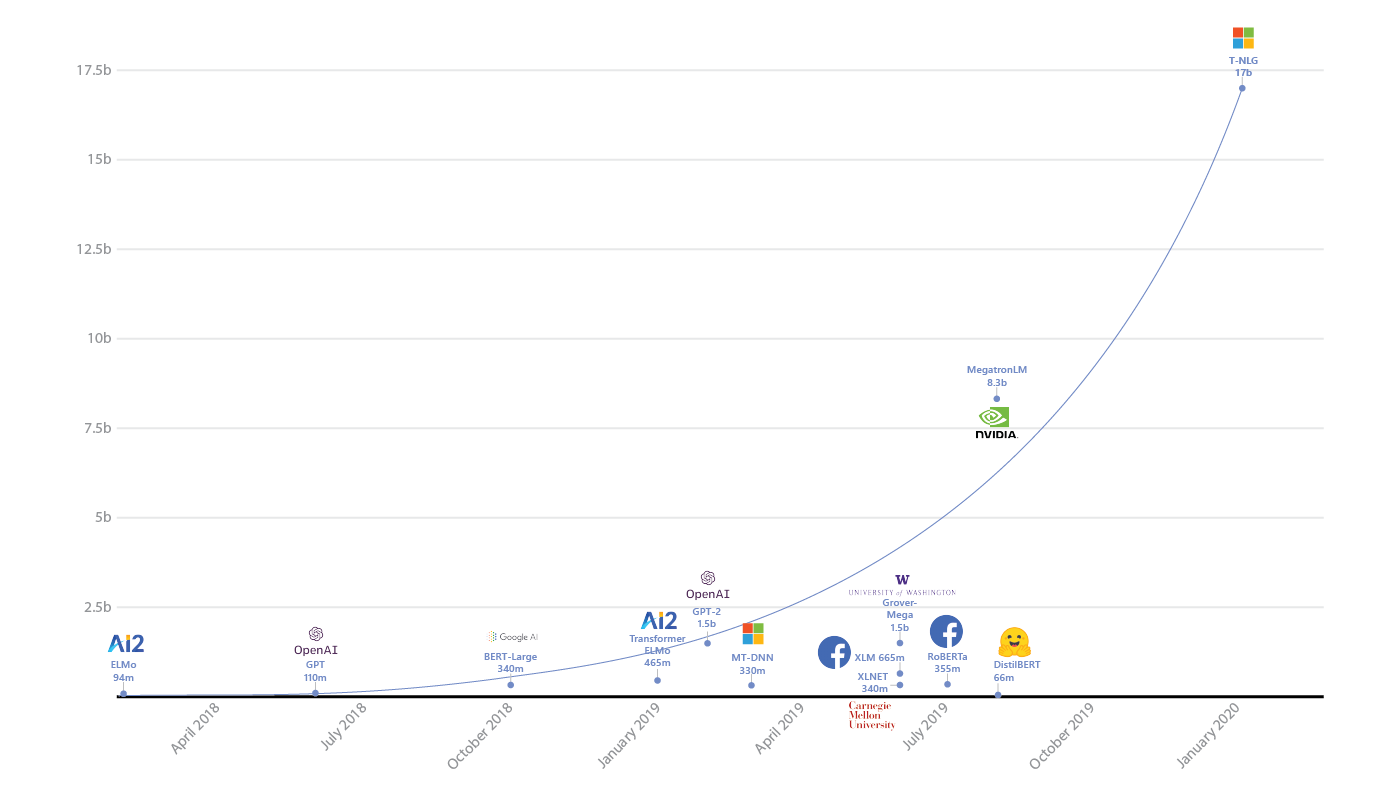
\includegraphics[width=0.7\columnwidth]{figures/beforegpt3}}
    \only<2>{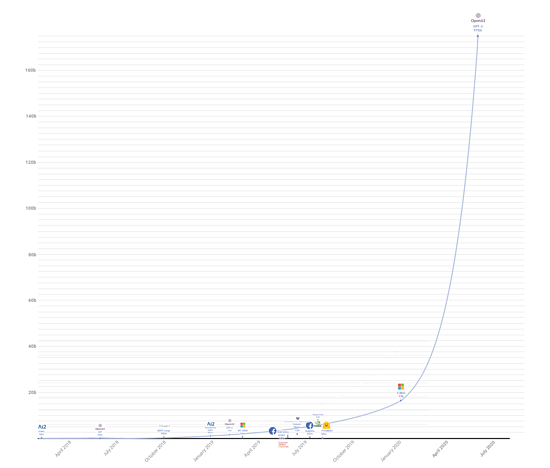
\includegraphics[width=0.4\columnwidth]{figures/gpt3}}
\end{frame}

\begin{frame}
    \frametitle{Towards transparency: latent variables}
    \fontsize{13pt}{15}\selectfont%
    \begin{itemize}
        \uncover<1->{\item Big models need big data, latent variables do not (inductive bias)}
        \uncover<2->{\item Big models are opaque, latent variables explain model's decisions}
        \uncover<3->{\item Big models are... Big! Latent variables may lead to smaller models}
    \end{itemize}
\end{frame}

\begin{frame}
    \frametitle{Latent variables in machine translation}
    \cornercite{brown1993mathematics}
    \centering
    
\includegraphics[width=0.5\columnwidth]{figures/alignments.pdf}
\end{frame}

\begin{frame}
    \frametitle{Latent variables in NMT}
    \centering
    \fontsize{15pt}{15}\selectfont%
    \begin{itemize}
        \uncover<1->{\item Advances in optimization $\rightarrow$ ditch latent
        variables}
        \uncover<2->{\item Good for high-resource language, fails
        in low-resource settings}
        \uncover<3->{\item Recent work uses variational inference to have latent variables in NMT}
    \end{itemize}
\end{frame}

\begin{frame}[t,plain,fragile]%
    \frametitle{A bit of context... On Seq2Seq}%
    \cornercite{bahdanau}%
    \begin{tikzpicture}[remember picture,overlay]
        \node[anchor=south east] at (current page.south east)
            {\scriptsize Slide Credit: Vlad Niculae\strut};
    \end{tikzpicture}
    \fontsize{13pt}{15}\selectfont%
    \begin{columns}[T]
    \begin{column}{.7\textwidth}%
    \begin{tikzpicture}[node distance=0pt]
    %
    \def\bottom{-7}%
    \def\top{0}%
    \foreach[count=\i] \j in {United,Nations,elections,end,today}{
        \node[word,anchor=south] (w\i) at (1.7*\i+2, \bottom) {\strut \alt<1-11>{\j}{}};
        \uncover<2->{\node[wvec,enc,above=-2pt of w\i] (embed\i) {};}
        \uncover<3->{
            \node[wvec,enc,above=6pt of embed\i] (enc\i) {};
            \path (embed\i) edge[netarrow] (enc\i);
        }
        \uncover<4->{\node[inner sep=0, outer sep=0, above=2pt of enc\i] (src\i){};}
        \uncover<4->{\draw[fill,attnedge] (src\i) circle[radius=1pt];}
    }
    \foreach[count=\i] \j in {Eleições,das,Nações,Unidas}
    {
        \pgfmathtruncatemacro\attnslideno{2*\i+2}
        \pgfmathtruncatemacro\outslideno{2*\i+3}
        \node[word,anchor=north, visible on=<\outslideno->] (y\i) at (1.7*\i+2, \top) {\strut \alt<1-11>{\j}{}};
        \node[wvec,dec,below=-2pt of y\i, visible on=<\outslideno->] (out\i) {};
        \node[wvec,dec,below=6pt of out\i, visible on=<\outslideno->] (dec\i) {};
        \node[wvec,attn,below=6pt of dec\i,visible on=<\attnslideno->] (attn\i) {};
        \node[inner sep=0, outer sep=0, below=2pt of attn\i] (trg\i) {};
        \draw[fill,attnedge,visible on=<\attnslideno->] (trg\i) circle[radius=1pt];
        \path (attn\i) edge[netarrow,visible on=<\outslideno->] (dec\i);
        \path (dec\i)  edge[netarrow,visible on=<\outslideno->] (out\i);
    }
    \node<4->[wvec,dec,left=14pt of dec1] (dec0) {};
    \node<4-> [anchor=west] at ([xshift=3pt]dec0.south west) {\scriptsize $\bs{s}_0$};
    \path<5-> (dec0) edge[netarrow] (dec1);
    % labels
    \node<2-> [anchor=west] at ([xshift=3pt]embed2.south west) {\scriptsize $\bs{v}_j$};
    \node<3-> [anchor=west] at ([xshift=3pt]enc2.south west) {\scriptsize $\bs{h}_j$};
    \node<4-> [anchor=west] at ([xshift=3pt]attn1.south west) {\scriptsize $\bs{c}_1$};
    \node<5-> [anchor=west] at ([xshift=3pt]dec1.south west) {\scriptsize $\bs{s}_1$};
    \node<5-> [anchor=west] at ([xshift=3pt]out1.south west) {\scriptsize $\bs{y}_1$};
    % encoder bi-LSTM arrows
    \def\sh{3pt}
    \uncover<3->{
    \path ([yshift=\sh]enc1.east)  edge[netarrow] ([yshift=\sh]enc2.west);
    \path ([yshift=\sh]enc2.east)  edge[netarrow] ([yshift=\sh]enc3.west);
    \path ([yshift=\sh]enc3.east)  edge[netarrow] ([yshift=\sh]enc4.west);
    \path ([yshift=\sh]enc4.east)  edge[netarrow] ([yshift=\sh]enc5.west);
    %
    \path ([yshift=-\sh]enc2.west) edge[netarrow] ([yshift=-\sh]enc1.east);
    \path ([yshift=-\sh]enc3.west) edge[netarrow] ([yshift=-\sh]enc2.east);
    \path ([yshift=-\sh]enc4.west) edge[netarrow] ([yshift=-\sh]enc3.east);
    \path ([yshift=-\sh]enc5.west) edge[netarrow] ([yshift=-\sh]enc4.east);
    }
    %
    % decoder LSTM arrows
    \uncover<7->{\path (dec1) edge[netarrow] (dec2);}
    \uncover<9->{\path (dec2) edge[netarrow] (dec3);}
    \uncover<11->{\path (dec3) edge[netarrow] (dec4);}
    % autoregressive arrows
    \uncover<7->{\path (out1) edge[netarrow] (dec2.north west);}
    \uncover<9->{\path (out2) edge[netarrow] (dec3.north west);}
    \uncover<11->{\path (out3) edge[netarrow] (dec4.north west);}
    
    % Attention to word 1
    \uncover<4->{
    \path (src1) edge[attnedge,opacity=.5] (trg1);
    \path (src2) edge[attnedge,opacity=.2] (trg1);
    \path (src3) edge[attnedge,opacity=.8] (trg1);
    \path (src4) edge[attnedge,opacity=.2] (trg1);
    \path (src5) edge[attnedge,opacity=.2] (trg1);
    }
%
\uncover<6->{
\path (src1) edge[attnedge,opacity=.6] (trg2);
\path (src2) edge[attnedge,opacity=.6] (trg2);
\path (src3) edge[attnedge,opacity=.4] (trg2);
\path (src4) edge[attnedge,opacity=.2] (trg2);
\path (src5) edge[attnedge,opacity=.2] (trg2);
}
%
\uncover<8->{
\path (src1) edge[attnedge,opacity=.4] (trg3);
\path (src2) edge[attnedge,opacity=.9] (trg3);
\path (src3) edge[attnedge,opacity=.2] (trg3);
\path (src4) edge[attnedge,opacity=.2] (trg3);
\path (src5) edge[attnedge,opacity=.2] (trg3);
}
%
\uncover<10->{
\path (src1) edge[attnedge,opacity=.9] (trg4);
\path (src2) edge[attnedge,opacity=.4] (trg4);
\path (src3) edge[attnedge,opacity=.2] (trg4);
\path (src4) edge[attnedge,opacity=.2] (trg4);
\path (src5) edge[attnedge,opacity=.2] (trg4);
}

\uncover<2->{\node[align=right,anchor=right, left=20pt of enc1] {Encoder};}
\uncover<4->{\node[align=right,anchor=right, left=20pt of attn1,yshift=-15pt]
    {Attention};}
\uncover<5->{\node[align=right,anchor=right, left=20pt of dec1] {Decoder};}
\end{tikzpicture}
\\
\end{column}
\begin{column}{.29\textwidth}%
\centering
\uncover<4->{
\textbf{\emph{attention weights}}
\\computed with \emph{softmax}:
\\[.5\baselineskip]
\small
for some decoder state $\bs{s}_t$,
compute contextually weighted average of input $\bs{c}_t$:
\begin{align*}
z_j &= \bs{s}_t^\top \bs{W}^{(a)}\bs{h}_j \\
\pi_j &= \operatorname{softmax}_j(\bs{z}) \\
\bs{c}_t &= \sum_j \pi_j \bs{h}_j
\end{align*}
}
\end{column}
\end{columns}
\end{frame}

\begin{frame}
    \frametitle{A bit of context... on Transformers}

    \fontsize{12pt}{15}\selectfont
    \only<1-5>{\cornercite{transf}}
    \only<6>{\cornercite{devlin2018bert}}
    \begin{columns}
    \uncover<1->{
        \hspace{2mm}\vspace{-1cm}\begin{column}{0.55\columnwidth}
            What if... Attention is all you need? \\
            \vspace{0.5cm}
    }
    \uncover<2->{
        {\color{myDarkYellow} Key idea:} Instead of Recurrent Neural Networks (RNNs), let's use attention mechanisms!
        \vspace{0.25cm}
    }
        \begin{itemize}
            \uncover<3->{\item In place of the RNNs, use self-attention}
            \uncover<4->{\item Do this with multiple heads (i.e. attention mechanisms in parallel)}
            \uncover<5->{\item ... and do it through several layers}
            \uncover<6->{\item Inspiration for big general-purpose models like BERT!}
        \end{itemize}
    \end{column}

    \begin{column}{0.4\columnwidth}
    \vspace{-1.5cm}
    \begin{center}
    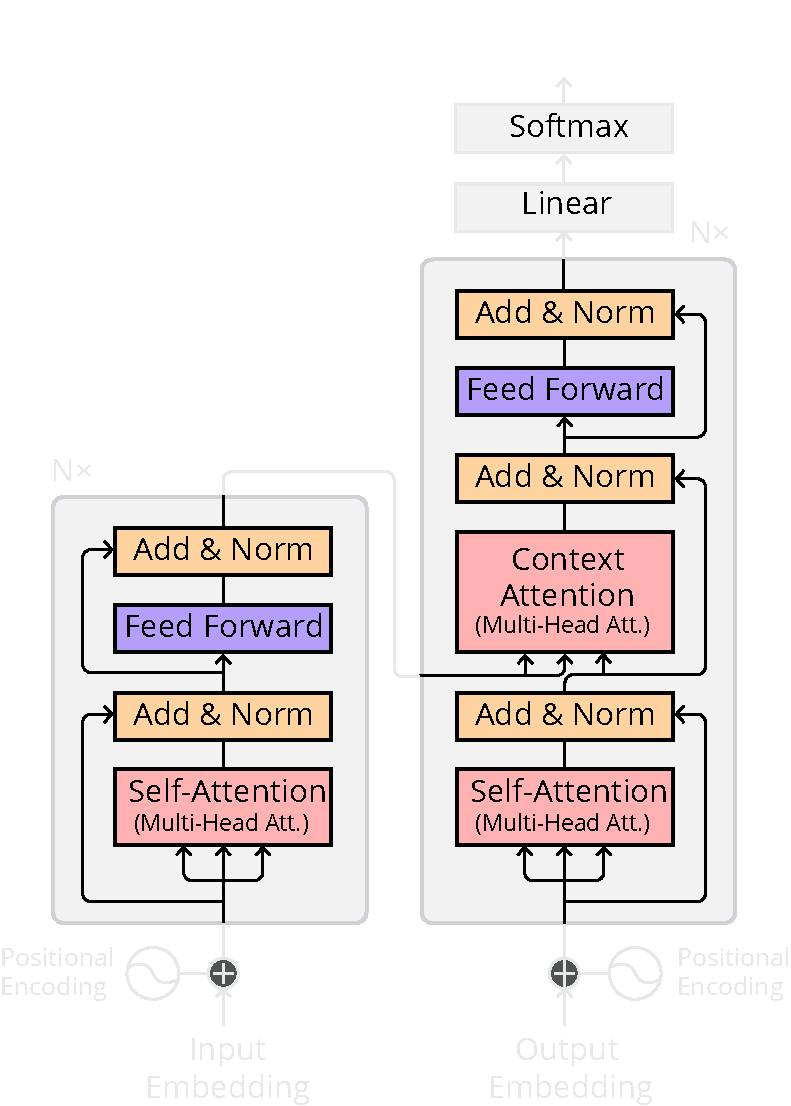
\includegraphics[width=0.8\columnwidth]{figures/transformer_mybg}
    \tikz[baseline,remember picture]{\node[anchor=base] (t1){};}
    \end{center}
    \end{column}
    \end{columns}

\end{frame}

\begin{frame}
    \frametitle{Outline}
    \fontsize{15pt}{15}\selectfont%
    \only<2>{\cornercite{myape2019}}
    \only<3>{\cornercite{mytransf2019}}
    \only<4>{\cornercite{myneurips2020}}
    \begin{itemize}
        \uncover<2->{\item Automatic Post-Editing (APE) using BERT (ACL 2019)}
        \uncover<3->{\item Letting Transformer learn how sparse it wants its attention (EMNLP 2019)}
        \uncover<4->{\item General strategy for efficient training discrete latent variables (NeurIPS 2020)}
        \uncover<5->{\item Future work: powerful structured latent variable models for NMT}
    \end{itemize}
\end{frame}

\section{A Simple and Effective Approach to Automatic Post-Editing with Transfer Learning}

\begin{frame}
    \frametitle{What is APE?}
    \centering
    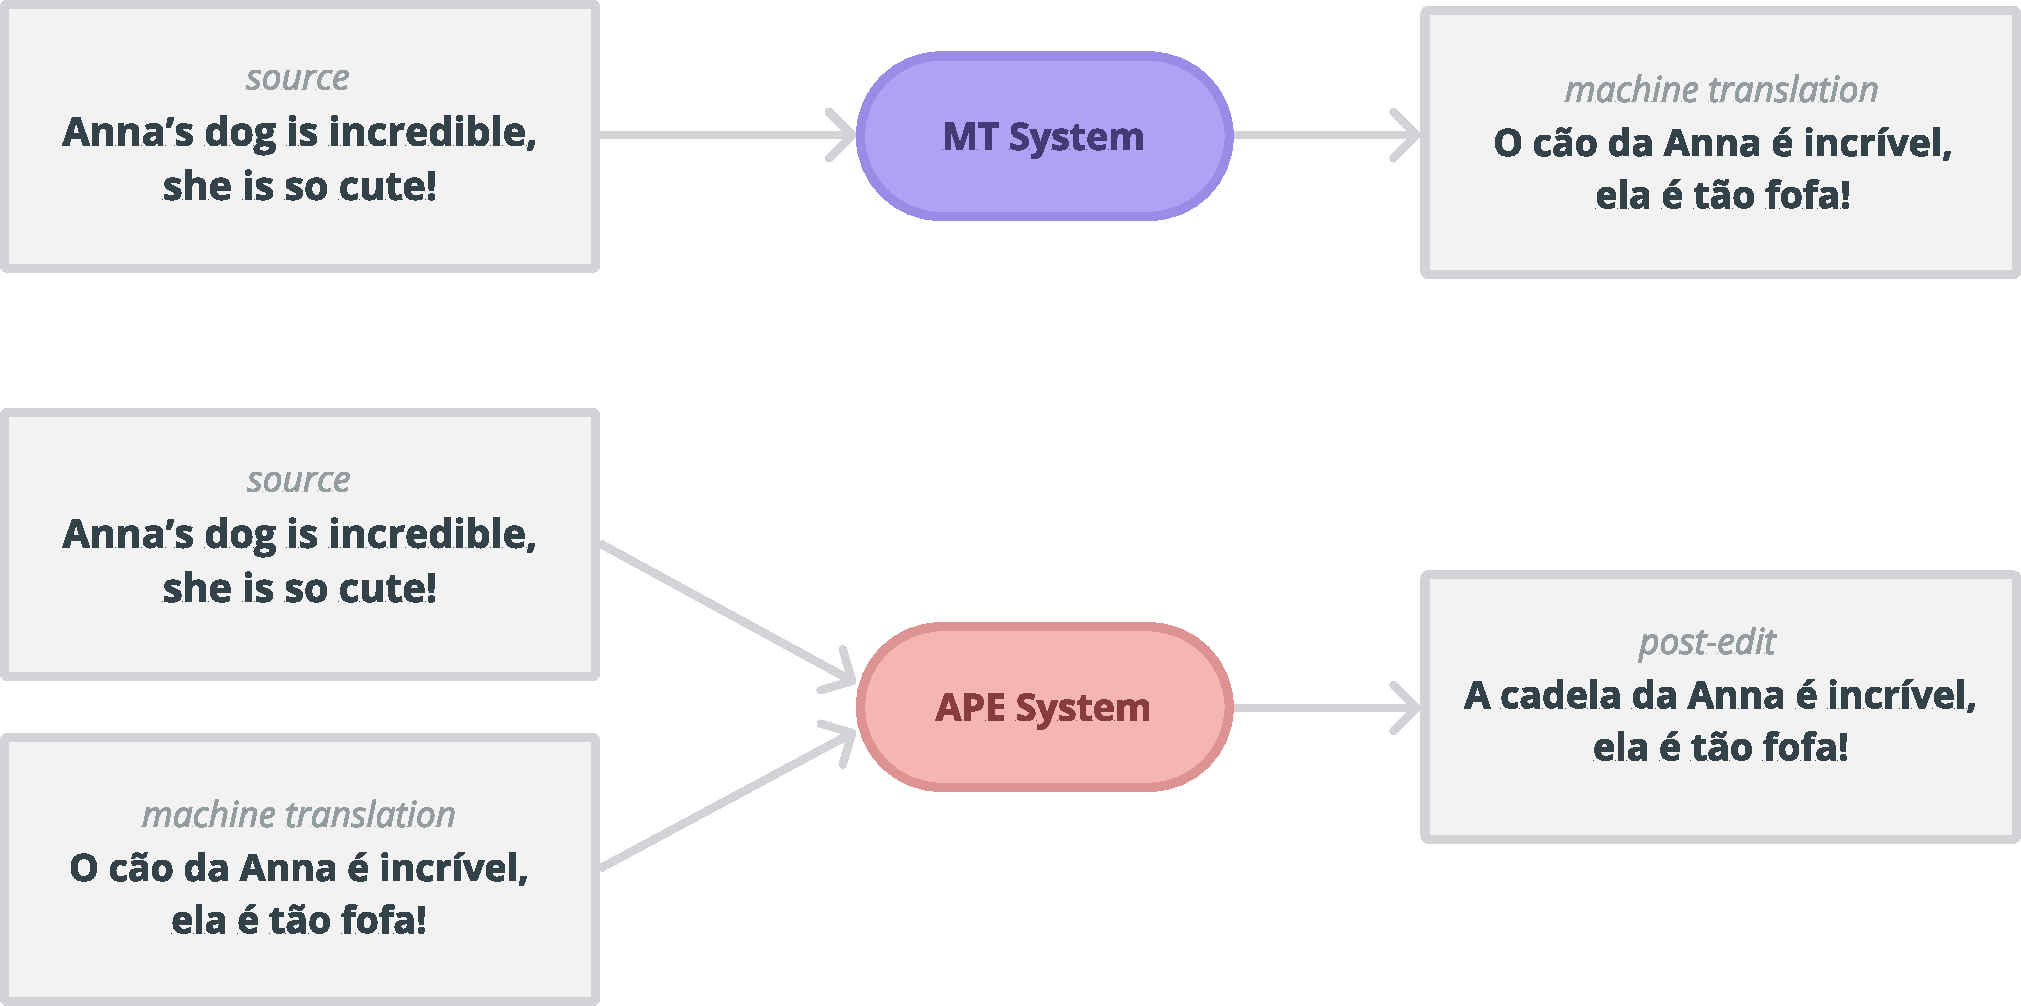
\includegraphics[width=0.8\columnwidth]{figures/ape.pdf}
\end{frame}

\begin{frame}
    \frametitle{BERT for APE}

    \fontsize{12pt}{15}\selectfont
    %\cornercite{transf}
    \begin{columns}
    \uncover<1->{
        \hspace{2mm}\vspace{-1cm}\begin{column}{0.55\columnwidth}
    }
    \uncover<2->{
        {\color{myDarkYellow} Key idea:} Use BERT to do APE
        \vspace{0.25cm}
    }
        \begin{itemize}
            \uncover<3->{\item Prior to this work, BERT was mainly used for simple classification tasks}
            \uncover<4->{\item We introduced an effective method to use BERT in a generation task (APE)}
            \uncover<5->{\item We achieved this via smart parameter sharing between encoder and decoder}
        \end{itemize}
    \end{column}

    \begin{column}{0.4\columnwidth}
    \vspace{-1.5cm}
    \begin{center}
    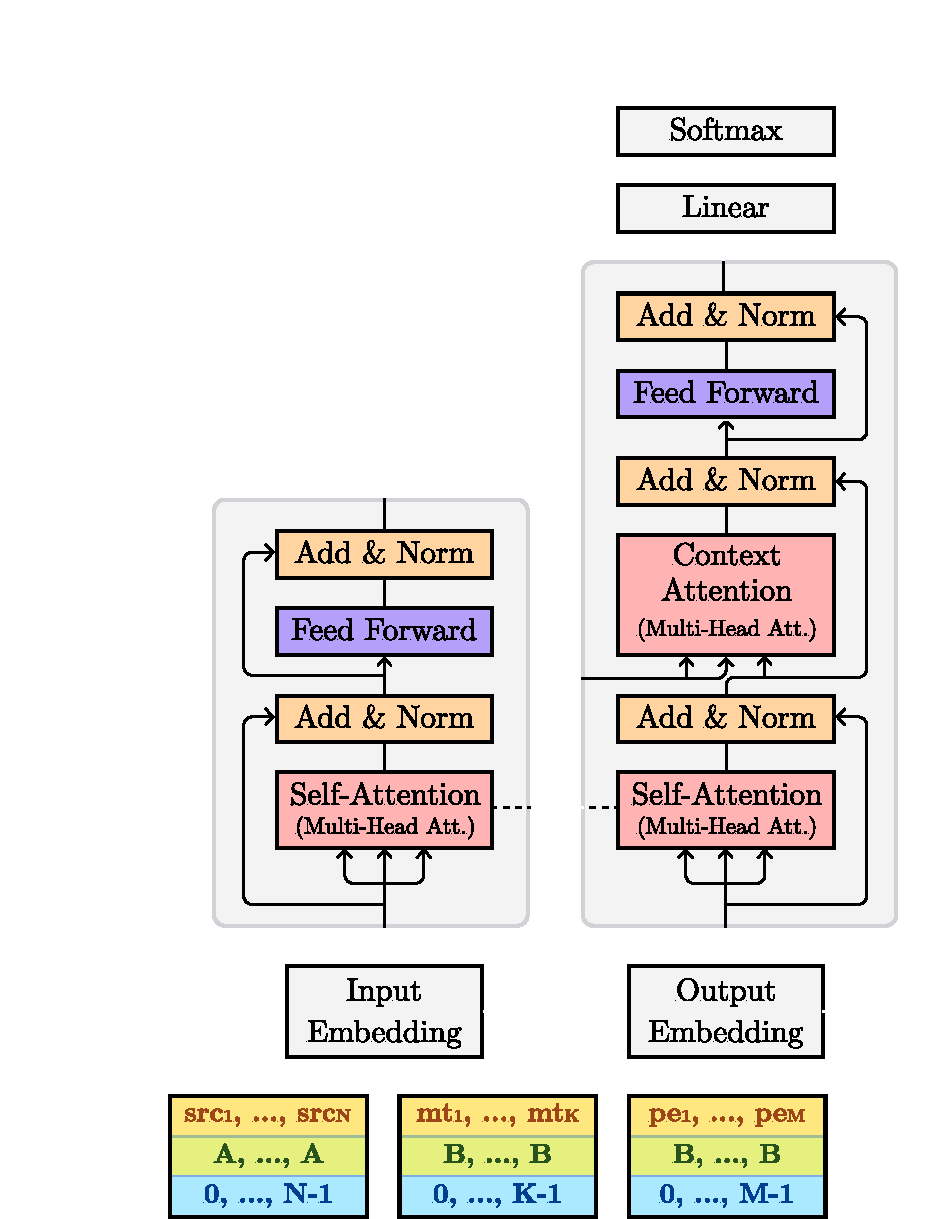
\includegraphics[width=0.8\columnwidth]{figures/bertape.pdf}
    \tikz[baseline,remember picture]{\node[anchor=base] (t1){};}
    \end{center}
    \end{column}
    \end{columns}
\end{frame}

% \begin{frame}\frametitle{Parameter sharing analysis}
%     \begin{table}[htbp]
%         \centering
%         \begin{tabular}{lcc}
%         \toprule
%          & TER$\downarrow$ & BLEU$\uparrow$ \\
%         MT Baseline & 24.76 & 62.11 \\
%         Transformer & 27.80 & 60.76 \\
%         \midrule
%         Transformer decoder & 20.33 & 69.31 \\
%         Pre-trained BERT & 20.83 & 69.11 \\
%         \hspace{1ex}\textcolor{gray}{\textit{with}}
%         CA $\leftarrow$ SA & 18.91 & 71.81 \\
%         \textover[r]
%         {\hspace{1ex}\textcolor{gray}{\textit{and}}}{\hspace{1ex}\textit{with}}
%         \textover[r]
%         {SA $\leftrightarrow$}
%         {CA $\leftarrow$} Encoder SA & \textbf{18.44} & \textbf{72.25} \\
%         \textover[r]
%         {\hspace{1ex}\textcolor{gray}{\textit{and}}}{\hspace{1ex}\textit{with}}
%         \textover[r]
%         {CA $\leftrightarrow$}{CA $\leftarrow$} SA & 18.75 & 71.83 \\
%         \textover[r]
%         {\hspace{1ex}\textcolor{gray}{\textit{and}}}{\hspace{1ex}\textit{with}}
%         \textover[r]
%         {FF $\leftrightarrow$}{CA $\leftarrow$} Encoder FF & 19.04 & 71.53 \\
%         \bottomrule
%         \end{tabular}
%             \label{tab:ablation_smt}
%     \end{table}
% \end{frame}

\section{Adaptively Sparse Transformers}

\begin{frame}
    \frametitle{Getting to know attention heads better}

    \begin{itemize}
        \uncover<1->{\item[] Attention heads may aid visualization but they are completely {\color{myDarkYellow} dense}.}
    \end{itemize}

    \bigskip

    \begin{itemize}
        \item[]<2-> Our solution is to bet on {\color{tPeony} sparsity}:
    \end{itemize}

    \begin{quote}
        {\normalfont
        \begin{itemize}
            \only<3>{\item {\color{myDarkYellow} for interpretability}}\only<2>{\item for interpretability} % sparse connections allow to be sure about which model representations were used to make a prediction
            \only<3>{\item {\color{myDarkYellow} for discovering linguistic structure}}\only<2>{\item for discovering linguistic structure} % we can redesign components based on what we find with sparsity
            \item<2-> for efficiency
        \end{itemize}}
    \end{quote}
\end{frame}

\begin{frame}
    \frametitle{
        \only<7->{{\color{myDarkYellow}Adaptively}} \only<5->{{\color{colorEntmax}Sparse}} \uncover<1->{Transformers}}

\only<1-4>{
    \fontsize{12pt}{15}\selectfont
    \cornercite{transf}
    \begin{columns}
    \hspace{2mm}\vspace{-1cm}\begin{column}{0.55\columnwidth}
    In each attention head:
    \begin{equation*}
    \bar{\matr{V}}  = \softmax\left(\frac{\matr{Q}\matr{K}^\top}{\sqrt{d_k}}\right)\matr{V}.
    \end{equation*}
    \uncover<2-4>{Attention in three places:
    \begin{itemize}
    \item Self-attention in the encoder\tikz[remember picture]{\node[coordinate] (n1) {};}}
    \uncover<3-4>{\item Self-attention in the decoder\tikz[remember picture]{\node[coordinate] (n2) {};}}
    \uncover<4>{\item Contextual attention\tikz[remember picture]{\node[coordinate] (n3) {};}}
    \end{itemize}

    % \vspace{-0.7cm}
    % \begin{align*}
    %     \uncover<2-4>{6 \text{ layers } \times 8 \text{ attention heads} &= 48}
    %     \\\uncover<3-4>{&+48}\\\only<4>{&+48=144\text{ attention heads}}
    % \end{align*}

    \end{column}
    \begin{column}{0.4\columnwidth}
    \vspace{-1.5cm}
    \begin{center}
    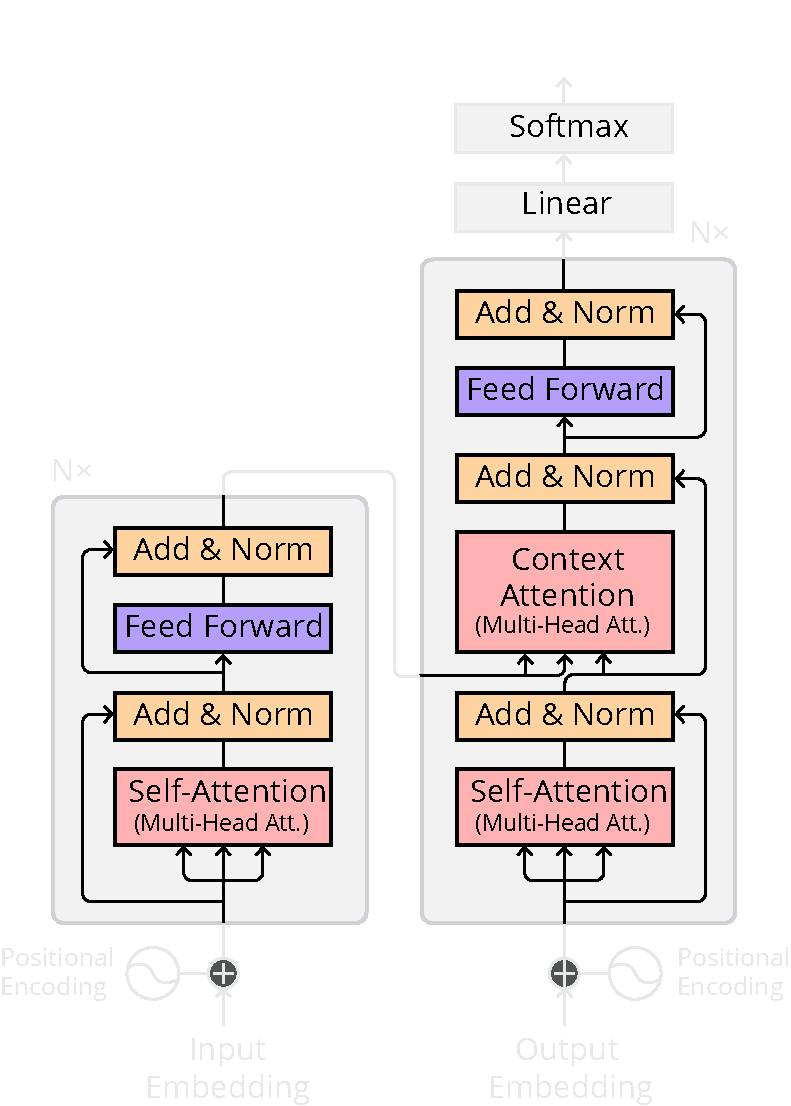
\includegraphics[width=0.9\columnwidth]{figures/transformer_mybg}
    \tikz[baseline,remember picture]{\node[anchor=base] (t1){};}
    \end{center}
    \end{column}
    \end{columns}

    \begin{tikzpicture}[remember picture,overlay]   %% use here too
        \uncover<2>{\path[draw=magenta,ultra thick,->](
            [xshift=2mm,yshift=1mm]n1.north) to [out=6cm,in=0,distance=-1.5cm] ([xshift=-5.13cm,yshift=2.0cm]t1.north);}
        \uncover<3>{\path[draw=magenta,ultra thick,->](
            [xshift=2mm,yshift=1mm]n2.north) to [out=6cm,in=0,distance=-3cm] ([xshift=-2.67cm,yshift=2.0cm]t1.north);}
        \uncover<4>{\path[draw=magenta,ultra thick,->](
            [xshift=2mm,yshift=1mm]n3.north) to [out=-6cm,in=0,distance=-2.5cm] ([xshift=-2.67cm,yshift=3.55cm]t1.north);}
    \end{tikzpicture}
}

\begin{itemize}
\item[]\uncover<6->{
    {\color{colorEntmax} Key idea:} replace softmax in attention heads by a sparse normalizing function! \quad\emoji{palms}
}

\bigskip

\item[]\uncover<7->{
    {\color{myDarkYellow} Another key idea:}
    use a normalizing function that is adaptively sparse via a learnable $\alpha$! \quad\emoji{palms}\enspace\emoji{palms}\enspace\emoji{palms}
}
\end{itemize}

\end{frame}

\begin{frame}[plain,t,fragile]%
    \frametitle{What is softmax?}%
    \centering \fontsize{12pt}{15}\selectfont
    Softmax exponentiates and normalizes:
    
    \begin{center}
    $\displaystyle
    \softmax(\xx_i) \defeq \frac{\exp \left(\xx_i\right)}{\sum_j \exp \left(\xx_j\right)}$
    \end{center}
    
    \bigskip

    \uncover<2->{
    {\color{myDarkYellow} It's fully dense: $\softmax(\vectsymb{z}) > \vect{0}$}}

\end{frame}

% \begin{frame}{$\Omega$-Regularized Argmax}
%     \cornercite{Niculae2017}
%     \fontsize{12pt}{15}\selectfont
%     \vspace{-0.5cm}
%     \begin{itemize}
%     \item[] For convex $\Omega$, define the {\bf $\Omega$-regularized argmax transformation}:\\
%     \bigskip
%     \begin{center}
%     $\displaystyle
%     \argmaxbf{}_{{\Omega}}(\vectsymb{z}) \defeq \arg\max_{\vectsymb{p} \in \triangle} \DP{\vectsymb{z}}{\vectsymb{p}} {\color{tPeony}- \Omega(\vectsymb{p})}$
%     \end{center}
%     \end{itemize}
%     \bigskip
%     \begin{itemize}
%     \uncover<2->{\item {\color{myDarkYellow} Argmax} corresponds to {\bf no regularization}, $\displaystyle\Omega \equiv 0$}
%     \uncover<3->{\item {\color{myDarkYellow} Softmax} amounts to {\bf entropic regularization}, $\displaystyle\Omega(\vectsymb{p}) = \sum_{i=1}^K p_i \log p_i$}
%     \uncover<4->{\item {\color{myDarkYellow} Sparsemax} amounts to {\bf $\ell_2$-regularization}, $\displaystyle\Omega(\vectsymb{p}) = \frac{1}{2}\|\vectsymb{p}\|^2$.}
%     \end{itemize}
%     \bigskip
%     \begin{itemize}
%     \item[] \uncover<5->{Is there something in-between?}
%     \end{itemize}
%     \uncover<4>{\cornercite[south east]{sparsemax}}
% \end{frame}

\begin{frame}{$\alpha$-Entmax}
    \cornercite{Peters2019ACL}
    \vspace{-1cm}
    \fontsize{12pt}{15}\selectfont
    \begin{itemize}
    \item[] Parametrized by {\color{tPeony}$\alpha \ge 0$}:
    \end{itemize}
    \bigskip
    % \begin{center}
    % $\displaystyle
    % \Omega_{{\color{tPeony}\alpha}}(\vectsymb{p}) \defeq 
    % \left\{
    % \begin{array}{ll}
    % \frac{1}{\alpha(\alpha-1)} \left(1 - \sum_{i=1}^K p_i^{\alpha}\right) & \text{if $\alpha \ne 1$}\\
    % \sum_{i=1}^K p_i\log p_i & \text{if $\alpha = 1$.}
    % \end{array}
    % \right.$
    % \end{center}
    % \bigskip
    \begin{itemize}
        \uncover<2->{\item {\bf Argmax} corresponds to {\color{tPeony}$\alpha \rightarrow \infty$}}
        \uncover<3->{\item {\bf Softmax} amounts to {\color{tPeony}$\alpha \rightarrow 1$}}
        \uncover<4->{\item {\bf Sparsemax} amounts to {\color{tPeony}$\alpha = 2$}.}
    \end{itemize}
    \bigskip
    \begin{itemize}
        \uncover<5->{\item[] {\color{myDarkYellow} Key result:} {\bf can be sparse for $\alpha > 1$}, propensity for sparsity increases with $\alpha$.}
    \end{itemize}

\end{frame}

\begin{frame}
    \centering
    % This file was created by tikzplotlib v0.8.5.
\begin{tikzpicture}

\definecolor{color0}{rgb}{0.63921568627451,0.658823529411765,0.635294117647059}
\definecolor{color1}{rgb}{0,0.709803921568627,0.83921568627451}
\definecolor{color2}{rgb}{0.552941176470588,0.827450980392157,0.780392156862745}
\definecolor{color3}{rgb}{0.890196078431372,0.384313725490196,0.486274509803922}
\definecolor{color4}{rgb}{0.866666666666667,0.850980392156863,0.72156862745098}
\definecolor{color5}{rgb}{0.466666666666667,0.498039215686275,0.458823529411765}

\begin{axis}[
width=0.9\columnwidth,
height=0.8\paperheight, 
axis line style={color0},
legend cell align={left},
legend style={
    nodes={scale=0.8, transform shape}, at={(0.97,0.3)}, anchor=east, draw=white!80.0!black, fill=myfg!30!mybg, fill opacity=0.6, draw opacity=1,text opacity=1},
tick align=outside,
tick pos=left,
x grid style={white!69.01960784313725!black},
xlabel={t},
xmin=-4.18, xmax=4.18,
xtick style={color=color0},
y grid style={white!69.01960784313725!black},
ymin=-0.05, ymax=1.05,
ytick style={color=color0}
]
\addplot [ultra thick, color1, dotted, visible on=<1->]
table {%
-3.8 0.0218797076995784
-3.79239239239239 0.0220431176990893
-3.78478478478478 0.0222077204139333
-3.77717717717718 0.0223735241350471
-3.76956956956957 0.02254053720296
-3.76196196196196 0.022708768011741
-3.75435435435435 0.0228782250060016
-3.74674674674675 0.0230489166826131
-3.73913913913914 0.023220851591204
-3.73153153153153 0.0233940383338884
-3.72392392392392 0.0235684855654955
-3.71631631631632 0.0237442019927435
-3.70870870870871 0.0239211963765537
-3.7011011011011 0.0240994775315149
-3.69349349349349 0.0242790543250429
-3.68588588588589 0.0244599356792074
-3.67827827827828 0.0246421305693472
-3.67067067067067 0.024825648024818
-3.66306306306306 0.0250104971303179
-3.65545545545546 0.0251966870250253
-3.64784784784785 0.025384226902531
-3.64024024024024 0.0255731260121778
-3.63263263263263 0.0257633936578743
-3.62502502502502 0.0259550392000158
-3.61741741741742 0.0261480720531249
-3.60980980980981 0.0263425016898114
-3.6022022022022 0.0265383376372378
-3.59459459459459 0.0267355894793524
-3.58698698698699 0.0269342668562215
-3.57937937937938 0.0271343794663349
-3.57177177177177 0.0273359370623263
-3.56416416416416 0.0275389494565811
-3.55655655655656 0.0277434265178456
-3.54894894894895 0.0279493781717068
-3.54134134134134 0.0281568144020211
-3.53373373373373 0.0283657452511388
-3.52612612612613 0.0285761808185395
-3.51851851851852 0.0287881312622743
-3.51091091091091 0.0290016068001401
-3.5033033033033 0.0292166177060302
-3.4956956956957 0.0294331743149346
-3.48808808808809 0.0296512870195949
-3.48048048048048 0.0298709662726378
-3.47287287287287 0.0300922225854518
-3.46526526526527 0.0303150665293606
-3.45765765765766 0.0305395087354829
-3.45005005005005 0.0307655598945752
-3.44244244244244 0.0309932307575462
-3.43483483483483 0.0312225321345982
-3.42722722722723 0.0314534748988601
-3.41961961961962 0.0316860699806737
-3.41201201201201 0.0319203283729567
-3.4044044044044 0.032156261129298
-3.3967967967968 0.0323938793641164
-3.38918918918919 0.0326331942531791
-3.38158158158158 0.0328742170330385
-3.37397397397397 0.0331169590011706
-3.36636636636637 0.0333614315183326
-3.35875875875876 0.0336076460042998
-3.35115115115115 0.0338556139443042
-3.34354354354354 0.0341053468821192
-3.33593593593594 0.03435685642427
-3.32832832832833 0.0346101542421185
-3.32072072072072 0.034865252065515
-3.31311311311311 0.0351221616890269
-3.30550550550551 0.0353808949690087
-3.2978978978979 0.0356414638252814
-3.29029029029029 0.0359038802384934
-3.28268268268268 0.0361681562545827
-3.27507507507507 0.0364343039801273
-3.26746746746747 0.0367023355868511
-3.25985985985986 0.0369722633072921
-3.25225225225225 0.037244099439367
-3.24464464464464 0.0375178563423836
-3.23703703703704 0.0377935464408404
-3.22942942942943 0.0380711822199333
-3.22182182182182 0.0383507762319267
-3.21421421421421 0.0386323410899314
-3.20660660660661 0.0389158894709048
-3.198998998999 0.0392014341166009
-3.19139139139139 0.0394889878314867
-3.18378378378378 0.0397785634836498
-3.17617617617618 0.0400701740066303
-3.16856856856857 0.0403638323950521
-3.16096096096096 0.0406595517095343
-3.15335335335335 0.0409573450731743
-3.14574574574575 0.0412572256742813
-3.13813813813814 0.0415592067636878
-3.13053053053053 0.0418633016570484
-3.12292292292292 0.0421695237325527
-3.11531531531532 0.0424778864341914
-3.10770770770771 0.0427884032685098
-3.1001001001001 0.0431010878055185
-3.09249249249249 0.0434159536806046
-3.08488488488488 0.0437330145911802
-3.07727727727728 0.0440522842995363
-3.06966966966967 0.0443737766308916
-3.06206206206206 0.0446975054743283
-3.05445445445445 0.0450234847837648
-3.04684684684685 0.0453517285739309
-3.03923923923924 0.0456822509273209
-3.03163163163163 0.0460150659825459
-3.02402402402402 0.0463501879473853
-3.01641641641642 0.0466876310953057
-3.00880880880881 0.0470274097524212
-3.0012012012012 0.0473695383212204
-2.99359359359359 0.0477140312550073
-2.98598598598599 0.04806090307497
-2.97837837837838 0.0484101683697262
-2.97077077077077 0.0487618417802252
-2.96316316316316 0.0491159380177959
-2.95555555555556 0.0494724718522275
-2.94794794794795 0.0498314581153683
-2.94034034034034 0.0501929117043252
-2.93273273273273 0.0505568475735747
-2.92512512512512 0.0509232807408625
-2.91751751751752 0.0512922262859585
-2.90990990990991 0.0516636993482092
-2.9023023023023 0.0520377151280267
-2.89469469469469 0.0524142888878628
-2.88708708708709 0.0527934359508798
-2.87947947947948 0.0531751716960219
-2.87187187187187 0.0535595115677392
-2.86426426426426 0.053946471066972
-2.85665665665666 0.0543360657556165
-2.84904904904905 0.0547283112520736
-2.84144144144144 0.0551232232363988
-2.83383383383383 0.0555208174458155
-2.82622622622623 0.0559211096768649
-2.81861861861862 0.0563241157826499
-2.81101101101101 0.056729851673111
-2.8034034034034 0.0571383333191261
-2.7957957957958 0.0575495767440118
-2.78818818818819 0.0579635980288171
-2.78058058058058 0.0583804133139655
-2.77297297297297 0.0588000387892192
-2.76536536536537 0.0592224907082006
-2.75775775775776 0.0596477853717613
-2.75015015015015 0.0600759391386485
-2.74254254254254 0.0605069684218627
-2.73493493493493 0.0609408896875703
-2.72732732732733 0.0613777194546562
-2.71971971971972 0.0618174742956382
-2.71211211211211 0.062260170834864
-2.7045045045045 0.0627058257466367
-2.6968968968969 0.0631544557616842
-2.68928928928929 0.063606077654848
-2.68168168168168 0.0640607082564316
-2.67407407407407 0.0645183644439932
-2.66646646646647 0.0649790631438923
-2.65885885885886 0.0654428213314613
-2.65125125125125 0.0659096560319284
-2.64364364364364 0.066379584314756
-2.63603603603604 0.0668526232981398
-2.62842842842843 0.0673287901462386
-2.62082082082082 0.0678081020670497
-2.61321321321321 0.06829057631703
-2.60560560560561 0.0687762301921844
-2.597997997998 0.0692650810357034
-2.59039039039039 0.0697571462327773
-2.58278278278278 0.0702524432091021
-2.57517517517518 0.0707509894340488
-2.56756756756757 0.071252802414493
-2.55995995995996 0.0717578997003455
-2.55235235235235 0.0722662988807092
-2.54474474474474 0.072778017579887
-2.53713713713714 0.0732930734638156
-2.52952952952953 0.0738114842295847
-2.52192192192192 0.0743332676168075
-2.51431431431431 0.0748584413953959
-2.50670670670671 0.075387023372081
-2.4990990990991 0.0759190313845911
-2.49149149149149 0.076454483304089
-2.48388388388388 0.0769933970351715
-2.47627627627628 0.0775357905107235
-2.46866866866867 0.078081681692644
-2.46106106106106 0.0786310885735
-2.45345345345345 0.0791840291729984
-2.44584584584585 0.0797405215378729
-2.43823823823824 0.0803005837391156
-2.43063063063063 0.0808642338736056
-2.42302302302302 0.0814314900604077
-2.41541541541542 0.0820023704442239
-2.40780780780781 0.0825768931880155
-2.4002002002002 0.0831550764782652
-2.39259259259259 0.0837369385156147
-2.38498498498498 0.0843224975238593
-2.37737737737738 0.0849117717423827
-2.36976976976977 0.0855047794230473
-2.36216216216216 0.0861015388394116
-2.35455455455455 0.0867020682713393
-2.34694694694695 0.0873063860141924
-2.33933933933934 0.087914510372828
-2.33173173173173 0.0885264596632377
-2.32412412412412 0.0891422522103308
-2.31651651651652 0.0897619063436635
-2.30890890890891 0.0903854404000488
-2.3013013013013 0.0910128727192391
-2.29369369369369 0.091644221647602
-2.28608608608609 0.0922795055286687
-2.27847847847848 0.092918742706734
-2.27087087087087 0.0935619515296079
-2.26326326326326 0.094209150337922
-2.25565565565566 0.0948603574687727
-2.24804804804805 0.0955155912542545
-2.24044044044044 0.0961748700210421
-2.23283283283283 0.0968382120824677
-2.22522522522523 0.0975056357497986
-2.21761761761762 0.0981771593135052
-2.21001001001001 0.098852801056718
-2.2024024024024 0.0995325792460845
-2.19479479479479 0.10021651213119
-2.18718718718719 0.100904617942879
-2.17957957957958 0.101596914894943
-2.17197197197197 0.102293421176828
-2.16436436436436 0.102994154956395
-2.15675675675676 0.103699134373616
-2.14914914914915 0.104408377549139
-2.14154154154154 0.105121902561745
-2.13393393393393 0.105839727477795
-2.12632632632633 0.106561870314517
-2.11871871871872 0.107288349066146
-2.11111111111111 0.108019181685626
-2.1035035035035 0.108754386094593
-2.0958958958959 0.109493980167071
-2.08828828828829 0.110237981740711
-2.08068068068068 0.110986408606362
-2.07307307307307 0.111739278518368
-2.06546546546547 0.112496609167864
-2.05785785785786 0.113258418212891
-2.05025025025025 0.114024723249029
-2.04264264264264 0.114795541826045
-2.03503503503504 0.115570891431931
-2.02742742742743 0.116350789499589
-2.01981981981982 0.117135253406062
-2.01221221221221 0.117924300458695
-2.0046046046046 0.118717947908479
-1.996996996997 0.119516212937464
-1.98938938938939 0.120319112656411
-1.98178178178178 0.121126664111832
-1.97417417417417 0.121938884269009
-1.96656656656657 0.122755790029832
-1.95895895895896 0.123577398204778
-1.95135135135135 0.124403725537689
-1.94374374374374 0.125234788684354
-1.93613613613614 0.126070604216887
-1.92852852852853 0.126911188618487
-1.92092092092092 0.127756558290835
-1.91331331331331 0.128606729536149
-1.90570570570571 0.129461718567351
-1.8980980980981 0.130321541499894
-1.89049049049049 0.13118621435063
-1.88288288288288 0.132055753038175
-1.87527527527528 0.132930173371547
-1.86766766766767 0.133809491057758
-1.86006006006006 0.13469372169781
-1.85245245245245 0.135582880772085
-1.84484484484484 0.136476983660075
-1.83723723723724 0.13737604561675
-1.82962962962963 0.138280081778777
-1.82202202202202 0.139189107161791
-1.81441441441441 0.140103136659201
-1.80680680680681 0.141022185037897
-1.7991991991992 0.141946266927577
-1.79159159159159 0.142875396839867
-1.78398398398398 0.143809589140387
-1.77637637637638 0.144748858056768
-1.76876876876877 0.145693217683834
-1.76116116116116 0.146642681967916
-1.75355355355355 0.147597264715212
-1.74594594594595 0.148556979570884
-1.73833833833834 0.149521840043903
-1.73073073073073 0.150491859481172
-1.72312312312312 0.151467051070985
-1.71551551551552 0.152447427843341
-1.70790790790791 0.153433002670359
-1.7003003003003 0.154423788251378
-1.69269269269269 0.155419797119994
-1.68508508508509 0.156421041639324
-1.67747747747748 0.157427534000667
-1.66986986986987 0.158439286209903
-1.66226226226226 0.159456310100016
-1.65465465465465 0.160478617321037
-1.64704704704705 0.161506219329706
-1.63943943943944 0.16253912740589
-1.63183183183183 0.163577352624343
-1.62422422422422 0.164620905871167
-1.61661661661662 0.1656697978371
-1.60900900900901 0.166724039008795
-1.6014014014014 0.167783639669184
-1.59379379379379 0.168848609892329
-1.58618618618619 0.169918959543851
-1.57857857857858 0.170994698281474
-1.57097097097097 0.172075835540412
-1.56336336336336 0.173162380537527
-1.55575575575576 0.174254342268023
-1.54814814814815 0.175351729504056
-1.54054054054054 0.176454550787535
-1.53293293293293 0.177562814432604
-1.52532532532533 0.178676528512463
-1.51771771771772 0.179795700869748
-1.51011011011011 0.180920339105327
-1.5025025025025 0.182050450570817
-1.4948948948949 0.183186042379237
-1.48728728728729 0.184327121387525
-1.47967967967968 0.185473694199098
-1.47207207207207 0.186625767176986
-1.46446446446446 0.187783346403352
-1.45685685685686 0.188946437713144
-1.44924924924925 0.190115046670008
-1.44164164164164 0.191289178575399
-1.43403403403403 0.192468838454637
-1.42642642642643 0.193654031061913
-1.41881881881882 0.194844760872614
-1.41121121121121 0.196041032077652
-1.4036036036036 0.19724284859741
-1.395995995996 0.198450214056661
-1.38838838838839 0.199663131791925
-1.38078078078078 0.200881604850288
-1.37317317317317 0.202105635979327
-1.36556556556557 0.203335227637092
-1.35795795795796 0.204570381973048
-1.35035035035035 0.205811100833565
-1.34274274274274 0.207057385760834
-1.33513513513514 0.208309237984922
-1.32752752752753 0.209566658427285
-1.31991991991992 0.210829647690478
-1.31231231231231 0.21209820605939
-1.3047047047047 0.213372333497898
-1.2970970970971 0.214652029645513
-1.28948948948949 0.21593729381403
-1.28188188188188 0.217228124986582
-1.27427427427427 0.218524521814344
-1.26666666666667 0.21982648261569
-1.25905905905906 0.221134005363144
-1.25145145145145 0.222447087697161
-1.24384384384384 0.223765726913178
-1.23623623623624 0.225089919955824
-1.22862862862863 0.226419663428119
-1.22102102102102 0.227754953575828
-1.21341341341341 0.229095786291726
-1.20580580580581 0.230442157115013
-1.1981981981982 0.231794061225673
-1.19059059059059 0.233151493446519
-1.18298298298298 0.234514448227193
-1.17537537537538 0.235882919656524
-1.16776776776777 0.237256901454366
-1.16016016016016 0.238636386973862
-1.15255255255255 0.240021369185239
-1.14494494494494 0.241411840691316
-1.13733733733734 0.242807793716709
-1.12972972972973 0.244209220099482
-1.12212212212212 0.245616111304432
-1.11451451451451 0.247028458404037
-1.10690690690691 0.248446252097469
-1.0992992992993 0.249869482677668
-1.09169169169169 0.251298140055969
-1.08408408408408 0.25273221375403
-1.07647647647648 0.254171692892758
-1.06886886886887 0.255616566212178
-1.06126126126126 0.257066822029307
-1.05365365365365 0.258522448283657
-1.04604604604605 0.259983432497821
-1.03843843843844 0.26144976180066
-1.03083083083083 0.262921422919294
-1.02322322322322 0.264398402159156
-1.01561561561562 0.265880685433675
-1.00800800800801 0.267368258235686
-1.0004004004004 0.268861105652753
-0.992792792792793 0.270359212365091
-0.985185185185185 0.271862562628432
-0.977577577577577 0.273371140283722
-0.96996996996997 0.274884928764191
-0.962362362362363 0.276403911087416
-0.954754754754755 0.277928069837938
-0.947147147147147 0.279457387192848
-0.93953953953954 0.280991844913993
-0.931931931931932 0.282531424330598
-0.924324324324324 0.284076106343482
-0.916716716716717 0.285625871454877
-0.909109109109109 0.287180699716414
-0.901501501501501 0.288740570768444
-0.893893893893894 0.290305463832402
-0.886286286286286 0.291875357690027
-0.878678678678678 0.293450230707605
-0.871071071071071 0.295030060818498
-0.863463463463463 0.296614825531532
-0.855855855855856 0.298204501933112
-0.848248248248248 0.299799066669507
-0.840640640640641 0.301398495975492
-0.833033033033033 0.303002765643433
-0.825425425425426 0.304611851045554
-0.817817817817818 0.306225727129799
-0.81021021021021 0.30784436840537
-0.802602602602603 0.309467748972546
-0.794994994994995 0.311095842480971
-0.787387387387387 0.312728622173499
-0.77977977977978 0.314366060858186
-0.772172172172172 0.316008130914545
-0.764564564564564 0.317654804303586
-0.756956956956957 0.319306052556963
-0.749349349349349 0.320961846783644
-0.741741741741742 0.322622157673276
-0.734134134134134 0.324286955488892
-0.726526526526527 0.325956210066697
-0.718918918918919 0.327629890841344
-0.711311311311311 0.329307966802584
-0.703703703703704 0.330990406538817
-0.696096096096096 0.332677178226626
-0.688488488488488 0.334368249616316
-0.680880880880881 0.336063588039439
-0.673273273273273 0.33776316043159
-0.665665665665666 0.339466933295634
-0.658058058058058 0.341174872754756
-0.65045045045045 0.342886944489142
-0.642842842842843 0.34460311380085
-0.635235235235235 0.346323345576871
-0.627627627627628 0.348047604301319
-0.62002002002002 0.349775854064141
-0.612412412412413 0.351508058546697
-0.604804804804805 0.353244181046143
-0.597197197197197 0.354984184461155
-0.58958958958959 0.356728031293086
-0.581981981981982 0.358475683675034
-0.574374374374374 0.360227103317794
-0.566766766766767 0.361982251594892
-0.559159159159159 0.36374108945244
-0.551551551551551 0.365503577494905
-0.543943943943944 0.367269675930673
-0.536336336336336 0.369039344597983
-0.528728728728729 0.370812542975143
-0.521121121121121 0.372589230166224
-0.513513513513514 0.374369364919589
-0.505905905905906 0.376152905601014
-0.498298298298298 0.377939810249953
-0.490690690690691 0.379730036536225
-0.483083083083083 0.381523541778987
-0.475475475475475 0.383320282944959
-0.467867867867868 0.385120216680796
-0.46026026026026 0.386923299269028
-0.452652652652653 0.388729486673371
-0.445045045045045 0.390538734511588
-0.437437437437437 0.392350998088545
-0.42982982982983 0.394166232373284
-0.422222222222222 0.395984392019382
-0.414614614614615 0.397805431363779
-0.407007007007007 0.399629304434407
-0.3993993993994 0.401455964953543
-0.391791791791792 0.403285366323309
-0.384184184184184 0.405117461678206
-0.376576576576577 0.40695220381706
-0.368968968968969 0.408789545300989
-0.361361361361361 0.410629438353405
-0.353753753753754 0.412471834949592
-0.346146146146146 0.414316686784463
-0.338538538538538 0.416163945271743
-0.330930930930931 0.418013561566281
-0.323323323323323 0.419865486554283
-0.315715715715716 0.421719670880683
-0.308108108108108 0.42357606493016
-0.300500500500501 0.425434618831205
-0.292892892892893 0.427295282488708
-0.285285285285285 0.429158005560162
-0.277677677677678 0.431022737464675
-0.27007007007007 0.43288942742099
-0.262462462462462 0.434758024409204
-0.254854854854855 0.436628477194432
-0.247247247247247 0.438500734336416
-0.23963963963964 0.44037474419442
-0.232032032032032 0.44225045492726
-0.224424424424424 0.444127814503128
-0.216816816816817 0.446006770689775
-0.209209209209209 0.447887271089123
-0.201601601601602 0.449769263117747
-0.193993993993994 0.451652694031906
-0.186386386386387 0.45353751092291
-0.178778778778779 0.455423660707225
-0.171171171171171 0.457311090167017
-0.163563563563564 0.459199745940642
-0.155955955955956 0.461089574507679
-0.148348348348348 0.462980522240323
-0.140740740740741 0.464872535337253
-0.133133133133133 0.466765559926782
-0.125525525525525 0.468659541985133
-0.117917917917918 0.470554427398886
-0.11031031031031 0.47245016194493
-0.102702702702703 0.474346691290885
-0.0950950950950951 0.476243961032447
-0.0874874874874876 0.478141916662525
-0.0798798798798801 0.480040503598139
-0.0722722722722722 0.481939667175772
-0.0646646646646647 0.483839352716325
-0.0570570570570572 0.485739505413538
-0.0494494494494493 0.487640070436215
-0.0418418418418418 0.489540992907754
-0.0342342342342343 0.49144221789599
-0.0266266266266268 0.493343690462933
-0.0190190190190189 0.495245355605582
-0.0114114114114114 0.497147158333241
-0.00380380380380396 0.499049043607984
0.00380380380380396 0.500950956394869
0.0114114114114114 0.502852841668525
0.0190190190190189 0.50475464439174
0.0266266266266264 0.506656309538451
0.0342342342342343 0.508557782100184
0.0418418418418418 0.510459007098197
0.0494494494494493 0.512359929567318
0.0570570570570572 0.514260494590688
0.0646646646646647 0.516160647277846
0.0722722722722722 0.518060332805474
0.0798798798798797 0.519959496418503
0.0874874874874876 0.521858083355788
0.0950950950950951 0.523756038971745
0.102702702702703 0.525653308708779
0.11031031031031 0.527549838051415
0.117917917917918 0.529445572590969
0.125525525525525 0.53134045800302
0.133133133133133 0.533234440077539
0.140740740740741 0.535127464660409
0.148348348348348 0.537019477772442
0.155955955955956 0.538910425485479
0.163563563563564 0.540800254053907
0.171171171171171 0.5426889098259
0.178778778778779 0.544576339297751
0.186386386386386 0.546462489084276
0.193993993993994 0.548347305967619
0.201601601601602 0.550230736885835
0.209209209209209 0.552112728914982
0.216816816816817 0.553993229312205
0.224424424424424 0.555872185497865
0.232032032032032 0.55774954506193
0.239639639639639 0.559625255795218
0.247247247247247 0.561499265658796
0.254854854854854 0.563371522802661
0.262462462462462 0.565241975590941
0.27007007007007 0.567110572577099
0.277677677677677 0.56897726253535
0.285285285285285 0.570841994441874
0.292892892892893 0.572704717512744
0.3005005005005 0.574565381165916
0.308108108108108 0.576423935065542
0.315715715715716 0.57828032910922
0.323323323323323 0.580134513440634
0.330930930930931 0.581986438436457
0.338538538538539 0.583836054731753
0.346146146146146 0.585683313213235
0.353753753753754 0.587528165051386
0.361361361361361 0.589370561647997
0.368968968968969 0.591210454707293
0.376576576576577 0.593047796176588
0.384184184184184 0.594882538330987
0.391791791791792 0.596714633680672
0.3993993993994 0.598544035055753
0.407007007007007 0.600370695559251
0.414614614614615 0.602194568632743
0.422222222222222 0.604015607982254
0.42982982982983 0.605833767630463
0.437437437437437 0.607649001909022
0.445045045045045 0.609461265484435
0.452652652652652 0.611270513329985
0.46026026026026 0.613076700731062
0.467867867867867 0.614879783324603
0.475475475475475 0.616679717050092
0.483083083083083 0.618476458223178
0.49069069069069 0.620269963465841
0.498298298298298 0.622060189745717
0.505905905905906 0.623847094395214
0.513513513513513 0.625630635089158
0.521121121121121 0.627410769828895
0.528728728728729 0.629187457023812
0.536336336336336 0.63096065539899
0.543943943943944 0.632730324076797
0.551551551551552 0.634496422511812
0.559159159159159 0.636258910551685
0.566766766766767 0.63801774841391
0.574374374374374 0.639772896676297
0.581981981981982 0.641524316331276
0.58958958958959 0.643271968705291
0.597197197197197 0.645015815541465
0.604804804804805 0.646755818954268
0.612412412412413 0.648491941455323
0.62002002002002 0.650224145943438
0.627627627627628 0.651952395694365
0.635235235235236 0.653676654422866
0.642842842842843 0.655396886192863
0.65045045045045 0.657113055515729
0.658058058058058 0.658825127252551
0.665665665665665 0.660533066698089
0.673273273273273 0.662236839570364
0.68088088088088 0.663936411955762
0.688488488488488 0.665631750386206
0.696096096096096 0.667322821769248
0.703703703703703 0.669009593458117
0.711311311311311 0.670692033203602
0.718918918918919 0.672370109172292
0.726526526526526 0.674043789927585
0.734134134134134 0.675713044515352
0.741741741741742 0.677377842325168
0.749349349349349 0.67903815321326
0.756956956956957 0.680693947445812
0.764564564564565 0.68234519570195
0.772172172172172 0.68399186908428
0.77977977977978 0.685633939144727
0.787387387387387 0.687271377819094
0.794994994994995 0.688904157513566
0.802602602602603 0.690532251031383
0.81021021021021 0.692155631582906
0.817817817817818 0.693774272872792
0.825425425425426 0.695388148956689
0.833033033033033 0.696997234358959
0.840640640640641 0.698601504029088
0.848248248248249 0.700200933328517
0.855855855855856 0.701795498071752
0.863463463463463 0.703385174466452
0.871071071071071 0.704969939177863
0.878678678678678 0.706549769292076
0.886286286286286 0.70812464231017
0.893893893893893 0.709694536173725
0.901501501501501 0.711259429227446
0.909109109109109 0.712819300292017
0.916716716716716 0.714374128555431
0.924324324324324 0.715923893653605
0.931931931931932 0.717468575672325
0.939539539539539 0.719008155077313
0.947147147147147 0.720542612795331
0.954754754754755 0.722071930159983
0.962362362362362 0.723596088921034
0.96996996996997 0.725115071237705
0.977577577577578 0.726628859720219
0.985185185185185 0.728137437382907
0.992792792792793 0.729640787645265
1.0004004004004 0.731138894341106
1.00800800800801 0.732631741768439
1.01561561561562 0.734119314568754
1.02322322322322 0.735601597841625
1.03083083083083 0.737078577088814
1.03843843843844 0.73855023819865
1.04604604604605 0.740016567504124
1.05365365365365 0.741477551726382
1.06126126126126 0.742933177975245
1.06886886886887 0.744383433791017
1.07647647647648 0.745828307095663
1.08408408408408 0.747267786251225
1.09169169169169 0.748701859952642
1.0992992992993 0.750130517327489
1.10690690690691 0.751553747903339
1.11451451451451 0.752971541583063
1.12212212212212 0.754383888686825
1.12972972972973 0.755790779893835
1.13733733733734 0.757192206284275
1.14494494494495 0.758588159297466
1.15255255255255 0.759978630816094
1.16016016016016 0.761363613023102
1.16776776776777 0.762743098536452
1.17537537537538 0.764117080341712
1.18298298298298 0.765485551766388
1.19059059059059 0.766848506547608
1.1981981981982 0.768205938764037
1.20580580580581 0.76955784288667
1.21341341341341 0.770904213718867
1.22102102102102 0.77224504643005
1.22862862862863 0.773580336572561
1.23623623623624 0.774910080029839
1.24384384384384 0.776234273076089
1.25145145145145 0.777552912289778
1.25905905905906 0.778865994630538
1.26666666666667 0.780173517378245
1.27427427427427 0.781475478175576
1.28188188188188 0.782771875010157
1.28948948948949 0.784062706179094
1.2970970970971 0.785347970349063
1.3047047047047 0.786627666494707
1.31231231231231 0.787901793932642
1.31991991991992 0.789170352303215
1.32752752752753 0.790433341569625
1.33513513513514 0.791690762008237
1.34274274274274 0.792942614242817
1.35035035035035 0.794188899164452
1.35795795795796 0.795429618027334
1.36556556556557 0.796664772359695
1.37317317317317 0.797894364015636
1.38078078078078 0.799118395147593
1.38838838838839 0.800336868205188
1.395995995996 0.801549785934079
1.4036036036036 0.802757151401526
1.41121121121121 0.803958967924
1.41881881881882 0.805155239137172
1.42642642642643 0.806345968932238
1.43403403403403 0.807531161535121
1.44164164164164 0.808710821424766
1.44924924924925 0.809884953322642
1.45685685685686 0.811053562290213
1.46446446446446 0.812216653592804
1.47207207207207 0.813374232824166
1.47967967967968 0.814526305787956
1.48728728728729 0.815672878613661
1.49489489489489 0.816813957619578
1.5025025025025 0.817949549438011
1.51011011011011 0.819079660895982
1.51771771771772 0.820204299122615
1.52532532532533 0.821323471484155
1.53293293293293 0.822437185564112
1.54054054054054 0.82354544920726
1.54814814814815 0.824648270499901
1.55575575575576 0.82574565773165
1.56336336336336 0.826837619467073
1.57097097097097 0.827924164461644
1.57857857857858 0.829005301715106
1.58618618618619 0.830081040451528
1.59379379379379 0.831151390108445
1.6014014014014 0.832216360335163
1.60900900900901 0.833275960991062
1.61661661661662 0.834330202153157
1.62422422422422 0.835379094123727
1.63183183183183 0.836422647373007
1.63943943943944 0.837460872593038
1.64704704704705 0.838493780668143
1.65465465465465 0.83952138268248
1.66226226226226 0.840543689899665
1.66986986986987 0.841560713788977
1.67747747747748 0.842572466004991
1.68508508508508 0.843578958357712
1.69269269269269 0.844580202876273
1.7003003003003 0.845576211751061
1.70790790790791 0.846566997331839
1.71551551551552 0.847552572154098
1.72312312312312 0.84853294892792
1.73073073073073 0.849508140517354
1.73833833833834 0.850478159947985
1.74594594594595 0.851443020424021
1.75355355355355 0.852402735288736
1.76116116116116 0.853357318022549
1.76876876876877 0.85430678231699
1.77637637637638 0.855251141940276
1.78398398398398 0.856190410868169
1.79159159159159 0.857124603168295
1.7991991991992 0.858053733064727
1.80680680680681 0.85897781496485
1.81441441441441 0.859896863343218
1.82202202202202 0.86081089283493
1.82962962962963 0.861719918224388
1.83723723723724 0.86262395437653
1.84484484484484 0.86352301633063
1.85245245245245 0.864417119221955
1.86006006006006 0.865306278308629
1.86766766766767 0.866190508940973
1.87527527527527 0.867069826636572
1.88288288288288 0.86794424697273
1.89049049049049 0.868813785651909
1.8980980980981 0.869678458499993
1.90570570570571 0.87053828143557
1.91331331331331 0.871393270468064
1.92092092092092 0.87224344170556
1.92852852852853 0.873088811372389
1.93613613613614 0.873929395788016
1.94374374374374 0.874765211316695
1.95135135135135 0.875596274452941
1.95895895895896 0.876422601790749
1.96656656656657 0.877244209982914
1.97417417417417 0.878061115729386
1.98178178178178 0.878873335902182
1.98938938938939 0.879680887338951
1.996996996997 0.880483787065533
2.0046046046046 0.881282052079466
2.01221221221221 0.882075699543638
2.01981981981982 0.882864746598736
2.02742742742743 0.883649210488639
2.03503503503504 0.884429108568671
2.04264264264264 0.885204458176327
2.05025025025025 0.885975276747236
2.05785785785786 0.886741581784089
2.06546546546546 0.887503390835268
2.07307307307307 0.888260721493103
2.08068068068068 0.88901359138228
2.08828828828829 0.889762018256855
2.0958958958959 0.89050601983085
2.1035035035035 0.891245613904851
2.11111111111111 0.891980818305102
2.11871871871872 0.892711650941252
2.12632632632633 0.893438129685854
2.13393393393393 0.894160272531252
2.14154154154154 0.894878097429325
2.14914914914915 0.895591622458604
2.15675675675676 0.896300865624006
2.16436436436436 0.897005845044036
2.17197197197197 0.89770657881996
2.17957957957958 0.898403085103867
2.18718718718719 0.899095382047274
2.19479479479479 0.899783487869397
2.2024024024024 0.900467420755794
2.21001001001001 0.901147198936646
2.21761761761762 0.901822840685318
2.22522522522523 0.902494364256808
2.23283283283283 0.903161787916177
2.24044044044044 0.903825129987205
2.24804804804805 0.904484408750634
2.25565565565566 0.905139642542976
2.26326326326326 0.905790849664693
2.27087087087087 0.906438048469136
2.27847847847848 0.907081257290761
2.28608608608609 0.907720494473822
2.29369369369369 0.908355778350783
2.3013013013013 0.908987127281209
2.30890890890891 0.909614559599939
2.31651651651652 0.910238093656018
2.32412412412412 0.910857747791128
2.33173173173173 0.911473540328059
2.33933933933934 0.912085489630048
2.34694694694695 0.912693613998226
2.35455455455455 0.913297931730918
2.36216216216216 0.913898461162899
2.36976976976977 0.91449522057283
2.37737737737738 0.915088228263058
2.38498498498498 0.915677502477084
2.39259259259259 0.916263061489663
2.4002002002002 0.916844923534403
2.40780780780781 0.917423106802389
2.41541541541542 0.917997629552944
2.42302302302302 0.918568509939257
2.43063063063063 0.919135766129313
2.43823823823824 0.91969941626391
2.44584584584585 0.92025947846562
2.45345345345345 0.920815970827357
2.46106106106106 0.921368911421369
2.46866866866867 0.921918318308278
2.47627627627628 0.922464209494962
2.48388388388388 0.92300660296403
2.49149149149149 0.923545516693164
2.4990990990991 0.924080968612984
2.50670670670671 0.924612976636637
2.51431431431431 0.925141558607335
2.52192192192192 0.925666732389598
2.52952952952953 0.926188515775742
2.53713713713714 0.926706926546379
2.54474474474474 0.927221982417904
2.55235235235235 0.927733701123718
2.55995995995996 0.928242100289622
2.56756756756757 0.928747197587209
2.57517517517517 0.929249010567962
2.58278278278278 0.92974755679616
2.59039039039039 0.930242853765353
2.597997997998 0.930734918959236
2.60560560560561 0.931223769799015
2.61321321321321 0.931709423683705
2.62082082082082 0.932191897937427
2.62842842842843 0.932671209849743
2.63603603603604 0.933147376705773
2.64364364364364 0.933620415681661
2.65125125125125 0.934090343967883
2.65885885885886 0.934557178664688
2.66646646646647 0.935020936853692
2.67407407407407 0.935481635555466
2.68168168168168 0.935939291738957
2.68928928928929 0.936393922341348
2.6968968968969 0.936845544246376
2.7045045045045 0.937294174241798
2.71211211211211 0.93773982917454
2.71971971971972 0.938182525710505
2.72732732732733 0.938622280552224
2.73493493493493 0.939059110313079
2.74254254254254 0.939493031578939
2.75015015015015 0.939924060865621
2.75775775775776 0.940352214628447
2.76536536536537 0.940777509292722
2.77297297297297 0.941199961200716
2.78058058058058 0.941619586694409
2.78818818818819 0.942036401968381
2.7957957957958 0.942450423267608
2.8034034034034 0.942861666688008
2.81101101101101 0.943270148322067
2.81861861861862 0.94367588421627
2.82622622622623 0.944078890317941
2.83383383383383 0.944479182537315
2.84144144144144 0.944876776767798
2.84904904904905 0.945271688748885
2.85665665665666 0.945663934254198
2.86426426426426 0.946053528933404
2.87187187187187 0.946440488426937
2.87947947947948 0.946824828302317
2.88708708708709 0.947206564053415
2.89469469469469 0.947585711110247
2.9023023023023 0.947962284869847
2.90990990990991 0.948336300664049
2.91751751751752 0.948707773716675
2.92512512512512 0.949076719269211
2.93273273273273 0.949443152432727
2.94034034034034 0.949807088303083
2.94794794794795 0.95016854188653
2.95555555555556 0.950527528162327
2.96316316316316 0.950884061997728
2.97077077077077 0.951238158231741
2.97837837837838 0.951589831642882
2.98598598598599 0.951939096906291
2.99359359359359 0.952285968762212
3.0012012012012 0.952630461698337
3.00880880880881 0.952972590234534
3.01641641641642 0.953312368922435
3.02402402402402 0.953649812037984
3.03163163163163 0.953984934035918
3.03923923923924 0.954317749094039
3.04684684684685 0.954648271409047
3.05445445445445 0.954976515206735
3.06206206206206 0.955302494508272
3.06966966966967 0.955626223362828
3.07727727727728 0.955947715688004
3.08488488488489 0.956266985396586
3.09249249249249 0.95658404630055
3.1001001001001 0.956898912174218
3.10770770770771 0.957211596721916
3.11531531531532 0.957522113545572
3.12292292292292 0.957830476261123
3.13053053053053 0.958136698338598
3.13813813813814 0.958440793229183
3.14574574574575 0.958742774311598
3.15335335335335 0.959042654912904
3.16096096096096 0.95934044828675
3.16856856856857 0.95963616759159
3.17617617617618 0.959929825986094
3.18378378378378 0.960221436500865
3.19139139139139 0.960511012165867
3.198998998999 0.960798565882068
3.20660660660661 0.961084110516944
3.21421421421421 0.961367658914767
3.22182182182182 0.961649223757443
3.22942942942943 0.96192881776686
3.23703703703704 0.962206453555073
3.24464464464464 0.962482143645188
3.25225225225225 0.962755900556442
3.25985985985986 0.963027736686269
3.26746746746747 0.96329766441678
3.27507507507508 0.963565696007454
3.28268268268268 0.963831843733784
3.29029029029029 0.964096119758563
3.2978978978979 0.964358536174262
3.30550550550551 0.964619105024072
3.31311311311311 0.964877838312267
3.32072072072072 0.965134747928867
3.32832832832833 0.96538984575639
3.33593593593594 0.96564314356237
3.34354354354354 0.96589465311689
3.35115115115115 0.966144386052887
3.35875875875876 0.966392353983732
3.36636636636637 0.966638568481485
3.37397397397397 0.966883040990714
3.38158158158158 0.967125782967667
3.38918918918919 0.967366805740426
3.3967967967968 0.967606120626669
3.4044044044044 0.967843738858203
3.41201201201201 0.968079671623612
3.41961961961962 0.968313930024976
3.42722722722723 0.968546525109786
3.43483483483483 0.968777467849149
3.44244244244244 0.969006769245052
3.45005005005005 0.969234440093443
3.45765765765766 0.969460491263615
3.46526526526527 0.96968493346123
3.47287287287287 0.969907777410982
3.48048048048048 0.970129033727157
3.48808808808809 0.970348712977944
3.4956956956957 0.970566825674403
3.5033033033033 0.970783382291753
3.51091091091091 0.970998393204461
3.51851851851852 0.971211868729058
3.52612612612613 0.971423819177814
3.53373373373373 0.971634254750666
3.54134134134134 0.971843185599654
3.54894894894895 0.972050621839469
3.55655655655656 0.972256573482474
3.56416416416416 0.97246105053558
3.57177177177177 0.972664062935272
3.57937937937938 0.972865620536561
3.58698698698699 0.973065733134336
3.59459459459459 0.97326441052796
3.6022022022022 0.973461662358999
3.60980980980981 0.973657498305471
3.61741741741742 0.973851927941163
3.62502502502502 0.974044960800256
3.63263263263263 0.974236606333857
3.64024024024024 0.974426873985496
3.64784784784785 0.974615773093575
3.65545545545546 0.974803312977701
3.66306306306306 0.974989502873563
3.67067067067067 0.975174351976019
3.67827827827828 0.97535786943891
3.68588588588589 0.975540064320719
3.69349349349349 0.975720945660178
3.7011011011011 0.97590052246527
3.70870870870871 0.976078803626372
3.71631631631632 0.976255798013559
3.72392392392392 0.976431514443932
3.73153153153153 0.976605961659753
3.73913913913914 0.976779148404157
3.74674674674675 0.976951083323411
3.75435435435435 0.977121774999246
3.76196196196196 0.977291231992076
3.76956956956957 0.97745946279745
3.77717717717718 0.977626475867583
3.78478478478478 0.97779227957863
3.79239239239239 0.977956882306511
3.8 0.97812029229648
};
\addlegendentry{$\alpha=1$ (softmax)}
\addplot [ultra thick, color2, visible on=<2->]
table {%
-3.8 6.24921888242048e-06
-3.79239239239239 7.25558404178219e-06
-3.78478478478478 8.3788475253669e-06
-3.77717717717718 9.62772462433999e-06
-3.76956956956957 1.10112429426343e-05
-3.76196196196196 1.25387422093411e-05
-3.75435435435435 1.42198740779046e-05
-3.74674674674675 1.60646019116799e-05
-3.73913913913914 1.8083200555414e-05
-3.73153153153153 2.02862560922136e-05
-3.72392392392392 2.26846655855606e-05
-3.71631631631632 2.52896368059443e-05
-3.70870870870871 2.81126879416729e-05
-3.7011011011011 3.11656472934362e-05
-3.69349349349349 3.44606529521867e-05
-3.68588588588589 3.80101524599174e-05
-3.67827827827828 4.18269024529032e-05
-3.67067067067067 4.59239682869863e-05
-3.66306306306306 5.03147236444878e-05
-3.65545545545546 5.50128501223207e-05
-3.64784784784785 6.00323368008919e-05
-3.64024024024024 6.53874797933765e-05
-3.63263263263263 7.10928817749601e-05
-3.62502502502502 7.71634514916334e-05
-3.61741741741742 8.36144032481354e-05
-3.60980980980981 9.04612563746485e-05
-3.6022022022022 9.77198346718423e-05
-3.59459459459459 0.000105406265833867
-3.58698698698699 0.000113536980848913
-3.57937937937938 0.000122128713376938
-3.57177177177177 0.000131198499104191
-3.56416416416416 0.000140763675074125
-3.55655655655656 0.00015084187899436
-3.54894894894895 0.000161451048519283
-3.54134134134134 0.000172609420507946
-3.53373373373373 0.000184335530256875
-3.52612612612613 0.000196648210707451
-3.51851851851852 0.000209566591627486
-3.51091091091091 0.000223110098766651
-3.5033033033033 0.000237298452985422
-3.4956956956957 0.000252151669357175
-3.48808808808809 0.000267690056243126
-3.48048048048048 0.000283934214339745
-3.47287287287287 0.000300905035698366
-3.46526526526527 0.000318623702716629
-3.45765765765766 0.000337111687101458
-3.45005005005005 0.000356390748803273
-3.44244244244244 0.000376482934921112
-3.43483483483483 0.000397410578578391
-3.42722722722723 0.000419196297768976
-3.41961961961962 0.000441862994173323
-3.41201201201201 0.000465433851944377
-3.4044044044044 0.000489932336462947
-3.3967967967968 0.000515382193062363
-3.38918918918919 0.000541807445722036
-3.38158158158158 0.000569232395729795
-3.37397397397397 0.000597681620312653
-3.36636636636637 0.000627179971235843
-3.35875875875876 0.000657752573369831
-3.35115115115115 0.000689424823225126
-3.34354354354354 0.000722222387454642
-3.33593593593594 0.000756171201323435
-3.32832832832833 0.000791297467145569
-3.32072072072072 0.000827627652687964
-3.31311311311311 0.000865188489541027
-3.30550550550551 0.000904006971455853
-3.2978978978979 0.000944110352647894
-3.29029029029029 0.000985526146066875
-3.28268268268268 0.00102828212163285
-3.27507507507507 0.00107240630443819
-3.26746746746747 0.00111792697291552
-3.25985985985986 0.0011648726569712
-3.25225225225225 0.00121327213608458
-3.24464464464464 0.00126315443737262
-3.23703703703704 0.00131454883361999
-3.22942942942943 0.00136748484127436
-3.22182182182182 0.00142199221840708
-3.21421421421421 0.00147810096263877
-3.20660660660661 0.00153584130903026
-3.198998998999 0.00159524372793834
-3.19139139139139 0.00165633892283663
-3.18378378378378 0.00171915782810133
-3.17617617617618 0.001783731606762
-3.16856856856857 0.00185009164821708
-3.16096096096096 0.00191826956591452
-3.15335335335335 0.00198829719499722
-3.14574574574575 0.00206020658991332
-3.13813813813814 0.00213403002199169
-3.13053053053053 0.00220979997698213
-3.12292292292292 0.00228754915256077
-3.11531531531532 0.00236731045580056
-3.10770770770771 0.00244911700060682
-3.1001001001001 0.00253300210511811
-3.09249249249249 0.00261899928907236
-3.08488488488488 0.00270714227113845
-3.07727727727728 0.00279746496621328
-3.06966966966967 0.00289000148268449
-3.06206206206206 0.0029847861196461
-3.05445445445445 0.00308185336414381
-3.04684684684685 0.00318123788825951
-3.03923923923924 0.00328297454628818
-3.03163163163163 0.00338709837181837
-3.02402402402402 0.00349364457479082
-3.01641641641642 0.0036026485385262
-3.00880880880881 0.00371414581671892
-3.0012012012012 0.00382817213039533
-2.99359359359359 0.00394476336484235
-2.98598598598599 0.00406395556650277
-2.97837837837838 0.0041857849398383
-2.97077077077077 0.0043102878441608
-2.96316316316316 0.00443750079043179
-2.95555555555556 0.0045674604380306
-2.94794794794795 0.00470020359149134
-2.94034034034034 0.00483576719720913
-2.93273273273273 0.00497418834011577
-2.92512512512512 0.00511550424032517
-2.91751751751752 0.0052597522497489
-2.90990990990991 0.00540696984868218
-2.9023023023023 0.00555719464236068
-2.89469469469469 0.00571046435748829
-2.88708708708709 0.00586681683873658
-2.87947947947948 0.00602629004521589
-2.87187187187187 0.00618892204691879
-2.86426426426426 0.00635475102113607
-2.85665665665666 0.00652381524884574
-2.84904904904905 0.00669615311107541
-2.84144144144144 0.00687180308523851
-2.83383383383383 0.00705080374144475
-2.82622622622623 0.00723319373878518
-2.81861861861862 0.00741901182159243
-2.81101101101101 0.00760829681567637
-2.8034034034034 0.00780108762453593
-2.7957957957958 0.00799742322554731
-2.78818818818819 0.00819734266612898
-2.78058058058058 0.00840088505988434
-2.77297297297297 0.00860808958272213
-2.76536536536537 0.00881899546895521
-2.75775775775776 0.0090336420073783
-2.75015015015015 0.00925206853732507
-2.74254254254254 0.00947431444470513
-2.73493493493493 0.00970041915802162
-2.72732732732733 0.00993042214436945
-2.71971971971972 0.0101643629054153
-2.71211211211211 0.0104022809733597
-2.7045045045045 0.0106442159068813
-2.6968968968969 0.0108902072870648
-2.68928928928929 0.0111402947133123
-2.68168168168168 0.011394517799239
-2.67407407407407 0.0116529161685535
-2.66646646646647 0.0119155294509242
-2.65885885885886 0.0121823972778307
-2.65125125125125 0.0124535592784027
-2.64364364364364 0.0127290550752457
-2.63603603603604 0.0130089242802541
-2.62842842842843 0.0132932064904138
-2.62082082082082 0.0135819412835924
-2.61321321321321 0.0138751682143199
-2.60560560560561 0.0141729268095594
-2.597997997998 0.0144752565644687
-2.59039039039039 0.0147821969381531
-2.58278278278278 0.0150937873494104
-2.57517517517518 0.0154100671724687
-2.56756756756757 0.0157310757327174
-2.55995995995996 0.0160568523024326
-2.55235235235235 0.0163874360964958
-2.54474474474474 0.0167228662681097
-2.53713713713714 0.0170631819045086
-2.52952952952953 0.0174084220226654
-2.52192192192192 0.0177586255649963
-2.51431431431431 0.0181138313950628
-2.50670670670671 0.0184740782932727
-2.4990990990991 0.0188394049525794
-2.49149149149149 0.0192098499741817
-2.48388388388388 0.0195854518632235
-2.47627627627628 0.019966249024495
-2.46866866866867 0.020352279758135
-2.46106106106106 0.0207435822553361
-2.45345345345345 0.0211401945940525
-2.44584584584585 0.0215421547347117
-2.43823823823824 0.0219495005159303
-2.43063063063063 0.0223622696502346
-2.42302302302302 0.0227804997197874
-2.41541541541542 0.0232042281721202
-2.40780780780781 0.023633492315873
-2.4002002002002 0.0240683293165407
-2.39259259259259 0.0245087761922289
-2.38498498498498 0.0249548698094172
-2.37737737737738 0.0254066468787331
-2.36976976976977 0.0258641439507346
-2.36216216216216 0.026327397411705
-2.35455455455455 0.0267964434794577
-2.34694694694695 0.0272713181991538
-2.33933933933934 0.0277520574391317
-2.33173173173173 0.0282386968867507
-2.32412412412412 0.0287312720442469
-2.31651651651652 0.0292298182246054
-2.30890890890891 0.0297343705474458
-2.3013013013013 0.0302449639349245
-2.29369369369369 0.0307616331076526
-2.28608608608609 0.031284412580631
-2.27847847847848 0.0318133366592022
-2.27087087087087 0.0323484394350978
-2.26326326326326 0.0328897547821222
-2.25565565565566 0.033437316352616
-2.24804804804805 0.0339911575731816
-2.24044044044044 0.0345513116408065
-2.23283283283283 0.0351178115189316
-2.22522522522523 0.0356906899335427
-2.21761761761762 0.0362699793692829
-2.21001001001001 0.0368557120655919
-2.2024024024024 0.0374479200128458
-2.19479479479479 0.0380466349485577
-2.18718718718719 0.0386518883535772
-2.17957957957958 0.0392637114483198
-2.17197197197197 0.0398821351890229
-2.16436436436436 0.0405071902640264
-2.15675675675676 0.0411389070900799
-2.14914914914915 0.0417773158086766
-2.14154154154154 0.0424224462824138
-2.13393393393393 0.0430743280913821
-2.12632632632633 0.0437329905295811
-2.11871871871872 0.0443984626013658
-2.11111111111111 0.0450707730179195
-2.1035035035035 0.0457499501937584
-2.0958958958959 0.0464360222432649
-2.08828828828829 0.0471290169772516
-2.08068068068068 0.0478289618995558
-2.07307307307307 0.048535884203666
-2.06546546546547 0.0492498107693791
-2.05785785785786 0.0499707681594901
-2.05025025025025 0.0506987826165144
-2.04264264264264 0.0514338800594422
-2.03503503503504 0.0521760860805275
-2.02742742742743 0.0529254259421089
-2.01981981981982 0.0536819245734658
-2.01221221221221 0.0544456065677087
-2.0046046046046 0.0552164961787032
-1.996996996997 0.0559946173180303
-1.98938938938939 0.0567799935519812
-1.98178178178178 0.0575726480985882
-1.97417417417417 0.0583726038246917
-1.96656656656657 0.0591798832430429
-1.95895895895896 0.0599945085094439
-1.95135135135135 0.0608165014199245
-1.94374374374374 0.0616458834079556
-1.93613613613614 0.0624826755417015
-1.92852852852853 0.063326898521308
-1.92092092092092 0.0641785726762307
-1.91331331331331 0.0650377179625995
-1.90570570570571 0.0659043539606237
-1.8980980980981 0.0667784998720343
-1.89049049049049 0.0676601745175656
-1.88288288288288 0.068549396334477
-1.87527527527528 0.0694461833741129
-1.86766766766767 0.0703505532995033
-1.86006006006006 0.0712625233830039
-1.85245245245245 0.072182110503976
-1.84484484484484 0.073109331146507
-1.83723723723724 0.0740442013971711
-1.82962962962963 0.0749867369428309
-1.82202202202202 0.0759369530684789
-1.81441441441441 0.0768948646551214
-1.80680680680681 0.0778604861777013
-1.7991991991992 0.0788338317030648
-1.79159159159159 0.0798149148879663
-1.78398398398398 0.0808037489771173
-1.77637637637638 0.0818003468012756
-1.76876876876877 0.0828047207753763
-1.76116116116116 0.0838168828967046
-1.75355355355355 0.0848368447431103
-1.74594594594595 0.0858646174712647
-1.73833833833834 0.0869002118149585
-1.73073073073073 0.0879436380834431
-1.72312312312312 0.0889949061598126
-1.71551551551552 0.0900540254994288
-1.70790790790791 0.0911210051283888
-1.7003003003003 0.0921958536420336
-1.69269269269269 0.0932785792034997
-1.68508508508509 0.0943691895423136
-1.67747747747748 0.0954676919530275
-1.66986986986987 0.0965740932938977
-1.66226226226226 0.0976883999856062
-1.65465465465465 0.0988106180100232
-1.64704704704705 0.0999407529090133
-1.63943943943944 0.101078809783283
-1.63183183183183 0.10222479329127
-1.62422422422422 0.10337870764808
-1.61661661661662 0.104540556624453
-1.60900900900901 0.10571034354579
-1.6014014014014 0.106888071291204
-1.59379379379379 0.108073742292628
-1.58618618618619 0.109267358533951
-1.57857857857858 0.11046892155021
-1.57097097097097 0.111678432426812
-1.56336336336336 0.112895891798808
-1.55575575575576 0.114121299850197
-1.54814814814815 0.115354656313285
-1.54054054054054 0.116595960468076
-1.53293293293293 0.117845211141708
-1.52532532532533 0.119102406707927
-1.51771771771772 0.120367545086612
-1.51011011011011 0.121640623743325
-1.5025025025025 0.122921639688922
-1.4948948948949 0.124210589479185
-1.48728728728729 0.12550746921451
-1.47967967967968 0.126812274539626
-1.47207207207207 0.128125000643361
-1.46446446446446 0.129445642258445
-1.45685685685686 0.130774193661354
-1.44924924924925 0.132110648672194
-1.44164164164164 0.133455000654625
-1.43403403403403 0.134807242515825
-1.42642642642643 0.136167366706493
-1.41881881881882 0.137535365220894
-1.41121121121121 0.138911229596938
-1.4036036036036 0.140294950916306
-1.395995995996 0.141686519804606
-1.38838838838839 0.143085926431575
-1.38078078078078 0.144493160511315
-1.37317317317317 0.145908211302571
-1.36556556556557 0.147331067609046
-1.35795795795796 0.14876171777975
-1.35035035035035 0.150200149709395
-1.34274274274274 0.151646350838818
-1.33513513513514 0.153100308155453
-1.32752752752753 0.154562008193827
-1.31991991991992 0.156031437036103
-1.31231231231231 0.15750858031266
-1.3047047047047 0.158993423202697
-1.2970970970971 0.160485950434893
-1.28948948948949 0.161986146288086
-1.28188188188188 0.163493994591996
-1.27427427427427 0.165009478727986
-1.26666666666667 0.16653258162985
-1.25905905905906 0.168063285784646
-1.25145145145145 0.169601573233554
-1.24384384384384 0.171147425572781
-1.23623623623624 0.172700823954488
-1.22862862862863 0.17426174908776
-1.22102102102102 0.175830181239608
-1.21341341341341 0.177406100236001
-1.20580580580581 0.17898948546294
-1.1981981981982 0.180580315867556
-1.19059059059059 0.182178569959246
-1.18298298298298 0.183784225810845
-1.17537537537538 0.185397261059824
-1.16776776776777 0.187017652909523
-1.16016016016016 0.18864537813042
-1.15255255255255 0.190280413061427
-1.14494494494494 0.19192273361122
-1.13733733733734 0.193572315259599
-1.12972972972973 0.195229133058882
-1.12212212212212 0.196893161635325
-1.11451451451451 0.198564375190582
-1.10690690690691 0.200242747503183
-1.0992992992993 0.20192825193005
-1.09169169169169 0.203620861408046
-1.08408408408408 0.205320548455542
-1.07647647647648 0.20702728517403
-1.06886886886887 0.208741043249744
-1.06126126126126 0.210461793955334
-1.05365365365365 0.212189508151547
-1.04604604604605 0.213924156288953
-1.03843843843844 0.215665708409685
-1.03083083083083 0.217414134149222
-1.02322322322322 0.219169402738185
-1.01561561561562 0.22093148300417
-1.00800800800801 0.222700343373606
-1.0004004004004 0.224475951873637
-0.992792792792793 0.226258276134034
-0.985185185185185 0.228047283389134
-0.977577577577577 0.229842940479798
-0.96996996996997 0.231645213855405
-0.962362362362363 0.233454069575865
-0.954754754754755 0.235269473313659
-0.947147147147147 0.237091390355906
-0.93953953953954 0.238919785606449
-0.931931931931932 0.240754623587973
-0.924324324324324 0.242595868444144
-0.916716716716717 0.244443483941771
-0.909109109109109 0.246297433472992
-0.901501501501501 0.248157680057595
-0.893893893893894 0.250024186344823
-0.886286286286286 0.251896914616265
-0.878678678678678 0.253775826787717
-0.871071071071071 0.255660884411589
-0.863463463463463 0.257552048679229
-0.855855855855856 0.259449280423271
-0.848248248248248 0.261352540120001
-0.840640640640641 0.26326178789175
-0.833033033033033 0.265176983509303
-0.825425425425426 0.267098086394335
-0.817817817817818 0.269025055621861
-0.81021021021021 0.27095784992271
-0.802602602602603 0.272896427686025
-0.794994994994995 0.274840746961772
-0.787387387387387 0.276790765463273
-0.77977977977978 0.278746440569769
-0.772172172172172 0.280707729328985
-0.764564564564564 0.282674588459724
-0.756956956956957 0.284646974354486
-0.749349349349349 0.286624843082087
-0.741741741741742 0.288608150390317
-0.734134134134134 0.290596851708604
-0.726526526526527 0.292590902150698
-0.718918918918919 0.294590256517375
-0.711311311311311 0.29659486929916
-0.703703703703704 0.298604694679058
-0.696096096096096 0.300619686535317
-0.688488488488488 0.302639798444194
-0.680880880880881 0.304664983682746
-0.673273273273273 0.306695195231632
-0.665665665665666 0.308730385777939
-0.658058058058058 0.310770507718013
-0.65045045045045 0.312815513160318
-0.642842842842843 0.314865353928298
-0.635235235235235 0.316919981563264
-0.627627627627628 0.318979347327291
-0.62002002002002 0.321043402206135
-0.612412412412413 0.323112096912157
-0.604804804804805 0.325185381887266
-0.597197197197197 0.327263207305877
-0.58958958958959 0.329345523077885
-0.581981981981982 0.331432278851641
-0.574374374374374 0.33352342401696
-0.566766766766767 0.335618907708126
-0.559159159159159 0.33771867880692
-0.551551551551551 0.339822685945654
-0.543943943943944 0.341930877510228
-0.536336336336336 0.344043201643187
-0.528728728728729 0.3461596062468
-0.521121121121121 0.348280038986144
-0.513513513513514 0.35040444729221
-0.505905905905906 0.352532778365007
-0.498298298298298 0.35466497917669
-0.490690690690691 0.356800996474692
-0.483083083083083 0.35894077678487
-0.475475475475475 0.361084266414663
-0.467867867867868 0.363231411456256
-0.46026026026026 0.36538215778976
-0.452652652652653 0.3675364510864
-0.445045045045045 0.369694236811714
-0.437437437437437 0.371855460228761
-0.42982982982983 0.374020066401337
-0.422222222222222 0.376188000197207
-0.414614614614615 0.37835920629134
-0.407007007007007 0.380533629169155
-0.3993993993994 0.38271121312978
-0.391791791791792 0.384891902289312
-0.384184184184184 0.387075640584096
-0.376576576576577 0.389262371774
-0.368968968968969 0.391452039445714
-0.361361361361361 0.39364458701604
-0.353753753753754 0.395839957735204
-0.346146146146146 0.398038094690168
-0.338538538538538 0.400238940807952
-0.330930930930931 0.402442438858967
-0.323323323323323 0.404648531460345
-0.315715715715716 0.406857161079289
-0.308108108108108 0.409068270036423
-0.300500500500501 0.411281800509144
-0.292892892892893 0.413497694534995
-0.285285285285285 0.415715894015029
-0.277677677677678 0.41793634071719
-0.27007007007007 0.420158976279692
-0.262462462462462 0.422383742214412
-0.254854854854855 0.424610579910283
-0.247247247247247 0.426839430636694
-0.23963963963964 0.429070235546899
-0.232032032032032 0.431302935681421
-0.224424424424424 0.433537471971477
-0.216816816816817 0.435773785242393
-0.209209209209209 0.438011816217032
-0.201601601601602 0.440251505519225
-0.193993993993994 0.442492793677205
-0.186386386386387 0.444735621127047
-0.178778778778779 0.446979928216111
-0.171171171171171 0.44922565520649
-0.163563563563564 0.451472742278459
-0.155955955955956 0.453721129533936
-0.148348348348348 0.455970756999931
-0.140740740740741 0.458221564632015
-0.133133133133133 0.460473492317784
-0.125525525525525 0.462726479880323
-0.117917917917918 0.464980467081682
-0.11031031031031 0.467235393626343
-0.102702702702703 0.469491199164704
-0.0950950950950951 0.47174782329655
-0.0874874874874876 0.474005205574539
-0.0798798798798801 0.47626328550768
-0.0722722722722722 0.478522002564822
-0.0646646646646647 0.480781296178139
-0.0570570570570572 0.483041105746616
-0.0494494494494493 0.485301370639808
-0.0418418418418418 0.487562030199854
-0.0342342342342343 0.48982302374829
-0.0266266266266268 0.492084290585713
-0.0190190190190189 0.494345769997565
-0.0114114114114114 0.49660740125704
-0.00380380380380396 0.498869123628588
0.00380380380380396 0.501130876371412
0.0114114114114114 0.50339259874296
0.0190190190190189 0.505654230002429
0.0266266266266264 0.507915709414255
0.0342342342342343 0.510176976251602
0.0418418418418418 0.512437969799859
0.0494494494494493 0.514698629360738
0.0570570570570572 0.516958894253384
0.0646646646646647 0.519218703821861
0.0722722722722722 0.521477997435178
0.0798798798798797 0.52373671449232
0.0874874874874876 0.525994794425461
0.0950950950950951 0.528252176703449
0.102702702702703 0.530508800835296
0.11031031031031 0.532764606373657
0.117917917917918 0.535019532918318
0.125525525525525 0.537273520119677
0.133133133133133 0.539526507682216
0.140740740740741 0.541778435367985
0.148348348348348 0.54402924300007
0.155955955955956 0.546278870466064
0.163563563563564 0.548527257721541
0.171171171171171 0.55077434479351
0.178778778778779 0.553020071783889
0.186386386386386 0.555264378872953
0.193993993993994 0.557507206322795
0.201601601601602 0.559748494480775
0.209209209209209 0.561988183782968
0.216816816816817 0.564226214757607
0.224424424424424 0.566462528028523
0.232032032032032 0.568697064318579
0.239639639639639 0.570929764453101
0.247247247247247 0.573160569363306
0.254854854854854 0.575389420089717
0.262462462462462 0.577616257785588
0.27007007007007 0.579841023720308
0.277677677677677 0.58206365928281
0.285285285285285 0.58428410598497
0.292892892892893 0.586502305465005
0.3005005005005 0.588718199490856
0.308108108108108 0.590931729963578
0.315715715715716 0.593142838920711
0.323323323323323 0.595351468539655
0.330930930930931 0.597557561141033
0.338538538538539 0.599761059192048
0.346146146146146 0.601961905309832
0.353753753753754 0.604160042264796
0.361361361361361 0.60635541298396
0.368968968968969 0.608547960554286
0.376576576576577 0.610737628226
0.384184184184184 0.612924359415904
0.391791791791792 0.615108097710688
0.3993993993994 0.61728878687022
0.407007007007007 0.619466370830845
0.414614614614615 0.62164079370866
0.422222222222222 0.623811999802793
0.42982982982983 0.625979933598663
0.437437437437437 0.628144539771239
0.445045045045045 0.630305763188286
0.452652652652652 0.6324635489136
0.46026026026026 0.634617842210241
0.467867867867867 0.636768588543744
0.475475475475475 0.638915733585337
0.483083083083083 0.64105922321513
0.49069069069069 0.643199003525308
0.498298298298298 0.64533502082331
0.505905905905906 0.647467221634993
0.513513513513513 0.64959555270779
0.521121121121121 0.651719961013855
0.528728728728729 0.6538403937532
0.536336336336336 0.655956798356813
0.543943943943944 0.658069122489772
0.551551551551552 0.660177314054346
0.559159159159159 0.66228132119308
0.566766766766767 0.664381092291874
0.574374374374374 0.66647657598304
0.581981981981982 0.668567721148359
0.58958958958959 0.670654476922116
0.597197197197197 0.672736792694123
0.604804804804805 0.674814618112735
0.612412412412413 0.676887903087844
0.62002002002002 0.678956597793865
0.627627627627628 0.681020652672709
0.635235235235236 0.683080018436737
0.642842842842843 0.685134646071702
0.65045045045045 0.687184486839682
0.658058058058058 0.689229492281987
0.665665665665665 0.691269614222061
0.673273273273273 0.693304804768368
0.68088088088088 0.695335016317254
0.688488488488488 0.697360201555806
0.696096096096096 0.699380313464683
0.703703703703703 0.701395305320942
0.711311311311311 0.70340513070084
0.718918918918919 0.705409743482625
0.726526526526526 0.707409097849303
0.734134134134134 0.709403148291397
0.741741741741742 0.711391849609683
0.749349349349349 0.713375156917914
0.756956956956957 0.715353025645515
0.764564564564565 0.717325411540276
0.772172172172172 0.719292270671016
0.77977977977978 0.721253559430231
0.787387387387387 0.723209234536727
0.794994994994995 0.725159253038229
0.802602602602603 0.727103572313975
0.81021021021021 0.72904215007729
0.817817817817818 0.73097494437814
0.825425425425426 0.732901913605665
0.833033033033033 0.734823016490697
0.840640640640641 0.73673821210825
0.848248248248249 0.738647459879999
0.855855855855856 0.740550719576729
0.863463463463463 0.742447951320771
0.871071071071071 0.744339115588411
0.878678678678678 0.746224173212283
0.886286286286286 0.748103085383735
0.893893893893893 0.749975813655177
0.901501501501501 0.751842319942406
0.909109109109109 0.753702566526671
0.916716716716716 0.755556516057907
0.924324324324324 0.75740413155555
0.931931931931932 0.759245376411735
0.939539539539539 0.761080214393273
0.947147147147147 0.76290860964383
0.954754754754755 0.764730526686089
0.962362362362362 0.766545930423896
0.96996996996997 0.768354786144369
0.977577577577578 0.770157059519987
0.985185185185185 0.771952716610662
0.992792792792793 0.773741723865772
1.0004004004004 0.77552404812618
1.00800800800801 0.777299656626221
1.01561561561562 0.779068516995666
1.02322322322322 0.780830597261661
1.03083083083083 0.782585865850632
1.03843843843844 0.784334291590177
1.04604604604605 0.786075843710917
1.05365365365365 0.78781049184833
1.06126126126126 0.78953820604455
1.06886886886887 0.791258956750147
1.07647647647648 0.792972714825868
1.08408408408408 0.794679451544361
1.09169169169169 0.796379138591864
1.0992992992993 0.798071748069865
1.10690690690691 0.799757252496738
1.11451451451451 0.801435624809343
1.12212212212212 0.803106838364605
1.12972972972973 0.804770866941053
1.13733733733734 0.806427684740339
1.14494494494495 0.808077266388722
1.15255255255255 0.809719586938519
1.16016016016016 0.81135462186953
1.16776776776777 0.812982347090431
1.17537537537538 0.814602738940133
1.18298298298298 0.816215774189114
1.19059059059059 0.817821430040716
1.1981981981982 0.819419684132409
1.20580580580581 0.821010514537027
1.21341341341341 0.822593899763968
1.22102102102102 0.824169818760364
1.22862862862863 0.825738250912214
1.23623623623624 0.827299176045488
1.24384384384384 0.828852574427196
1.25145145145145 0.830398426766425
1.25905905905906 0.831936714215335
1.26666666666667 0.833467418370131
1.27427427427427 0.834990521271997
1.28188188188188 0.836506005407989
1.28948948948949 0.8380138537119
1.2970970970971 0.839514049565094
1.3047047047047 0.841006576797291
1.31231231231231 0.842491419687329
1.31991991991992 0.843968562963886
1.32752752752753 0.845437991806164
1.33513513513514 0.846899691844539
1.34274274274274 0.848353649161174
1.35035035035035 0.849799850290598
1.35795795795796 0.851238282220243
1.36556556556557 0.852668932390948
1.37317317317317 0.854091788697423
1.38078078078078 0.85550683948868
1.38838838838839 0.85691407356842
1.395995995996 0.85831348019539
1.4036036036036 0.85970504908369
1.41121121121121 0.861088770403058
1.41881881881882 0.862464634779103
1.42642642642643 0.863832633293504
1.43403403403403 0.865192757484172
1.44164164164164 0.866544999345372
1.44924924924925 0.867889351327803
1.45685685685686 0.869225806338644
1.46446446446446 0.870554357741553
1.47207207207207 0.871874999356638
1.47967967967968 0.873187725460373
1.48728728728729 0.874492530785489
1.49489489489489 0.875789410520813
1.5025025025025 0.877078360311076
1.51011011011011 0.878359376256673
1.51771771771772 0.879632454913387
1.52532532532533 0.880897593292072
1.53293293293293 0.882154788858291
1.54054054054054 0.883404039531923
1.54814814814815 0.884645343686714
1.55575575575576 0.885878700149803
1.56336336336336 0.887104108201192
1.57097097097097 0.888321567573187
1.57857857857858 0.88953107844979
1.58618618618619 0.890732641466049
1.59379379379379 0.891926257707372
1.6014014014014 0.893111928708795
1.60900900900901 0.89428965645421
1.61661661661662 0.895459443375547
1.62422422422422 0.89662129235192
1.63183183183183 0.897775206708729
1.63943943943944 0.898921190216717
1.64704704704705 0.900059247090987
1.65465465465465 0.901189381989977
1.66226226226226 0.902311600014393
1.66986986986987 0.903425906706102
1.67747747747748 0.904532308046972
1.68508508508508 0.905630810457686
1.69269269269269 0.9067214207965
1.7003003003003 0.907804146357966
1.70790790790791 0.908878994871611
1.71551551551552 0.909945974500571
1.72312312312312 0.911005093840188
1.73073073073073 0.912056361916557
1.73833833833834 0.913099788185041
1.74594594594595 0.914135382528735
1.75355355355355 0.91516315525689
1.76116116116116 0.916183117103295
1.76876876876877 0.917195279224624
1.77637637637638 0.918199653198724
1.78398398398398 0.919196251022883
1.79159159159159 0.920185085112034
1.7991991991992 0.921166168296935
1.80680680680681 0.922139513822298
1.81441441441441 0.923105135344879
1.82202202202202 0.924063046931521
1.82962962962963 0.925013263057169
1.83723723723724 0.925955798602829
1.84484484484484 0.926890668853493
1.85245245245245 0.927817889496024
1.86006006006006 0.928737476616996
1.86766766766767 0.929649446700497
1.87527527527527 0.930553816625887
1.88288288288288 0.931450603665523
1.89049049049049 0.932339825482435
1.8980980980981 0.933221500127966
1.90570570570571 0.934095646039376
1.91331331331331 0.9349622820374
1.92092092092092 0.93582142732377
1.92852852852853 0.936673101478692
1.93613613613614 0.937517324458299
1.94374374374374 0.938354116592045
1.95135135135135 0.939183498580076
1.95895895895896 0.940005491490556
1.96656656656657 0.940820116756957
1.97417417417417 0.941627396175308
1.98178178178178 0.942427351901412
1.98938938938939 0.943220006448019
1.996996996997 0.944005382681969
2.0046046046046 0.944783503821297
2.01221221221221 0.945554393432291
2.01981981981982 0.946318075426534
2.02742742742743 0.947074574057891
2.03503503503504 0.947823913919472
2.04264264264264 0.948566119940558
2.05025025025025 0.949301217383486
2.05785785785786 0.95002923184051
2.06546546546546 0.950750189230621
2.07307307307307 0.951464115796334
2.08068068068068 0.952171038100444
2.08828828828829 0.952870983022749
2.0958958958959 0.953563977756735
2.1035035035035 0.954250049806242
2.11111111111111 0.954929226982081
2.11871871871872 0.955601537398634
2.12632632632633 0.956267009470419
2.13393393393393 0.956925671908618
2.14154154154154 0.957577553717586
2.14914914914915 0.958222684191324
2.15675675675676 0.95886109290992
2.16436436436436 0.959492809735973
2.17197197197197 0.960117864810977
2.17957957957958 0.96073628855168
2.18718718718719 0.961348111646423
2.19479479479479 0.961953365051442
2.2024024024024 0.962552079987154
2.21001001001001 0.963144287934408
2.21761761761762 0.963730020630717
2.22522522522523 0.964309310066542
2.23283283283283 0.964882188481245
2.24044044044044 0.965448688359453
2.24804804804805 0.966008842427154
2.25565565565566 0.966562683647787
2.26326326326326 0.967110245218344
2.27087087087087 0.967651560565425
2.27847847847848 0.96818666334032
2.28608608608609 0.968715587418938
2.29369369369369 0.969238366891959
2.3013013013013 0.969755036064725
2.30890890890891 0.970265629452239
2.31651651651652 0.970770181775111
2.32412412412412 0.971268727955498
2.33173173173173 0.97176130311302
2.33933933933934 0.972247942560663
2.34694694694695 0.972728681800661
2.35455455455455 0.973203556520376
2.36216216216216 0.973672602588146
2.36976976976977 0.974135856049132
2.37737737737738 0.974593353121147
2.38498498498498 0.975045130190476
2.39259259259259 0.975491223807676
2.4002002002002 0.975931670683374
2.40780780780781 0.976366507684051
2.41541541541542 0.976795771827812
2.42302302302302 0.977219500280152
2.43063063063063 0.977637730349711
2.43823823823824 0.978050499484021
2.44584584584585 0.978457845265245
2.45345345345345 0.97885980540591
2.46106106106106 0.97925641774463
2.46866866866867 0.979647720241835
2.47627627627628 0.980033750975478
2.48388388388388 0.980414548136753
2.49149149149149 0.980790150025797
2.4990990990991 0.981160595047402
2.50670670670671 0.98152592170671
2.51431431431431 0.981886168604922
2.52192192192192 0.982241374434991
2.52952952952953 0.982591577977323
2.53713713713714 0.982936818095481
2.54474474474474 0.983277133731881
2.55235235235235 0.983612563903496
2.55995995995996 0.98394314769756
2.56756756756757 0.984268924267276
2.57517517517517 0.984589932827526
2.58278278278278 0.984906212650585
2.59039039039039 0.985217803061843
2.597997997998 0.985524743435528
2.60560560560561 0.985827073190437
2.61321321321321 0.986124831785678
2.62082082082082 0.986418058716405
2.62842842842843 0.986706793509584
2.63603603603604 0.986991075719744
2.64364364364364 0.987270944924753
2.65125125125125 0.987546440721596
2.65885885885886 0.987817602722168
2.66646646646647 0.988084470549075
2.67407407407407 0.988347083831445
2.68168168168168 0.98860548220076
2.68928928928929 0.988859705286687
2.6968968968969 0.989109792712934
2.7045045045045 0.989355784093118
2.71211211211211 0.98959771902664
2.71971971971972 0.989835637094584
2.72732732732733 0.99006957785563
2.73493493493493 0.990299580841978
2.74254254254254 0.990525685555295
2.75015015015015 0.990747931462674
2.75775775775776 0.990966357992621
2.76536536536537 0.991181004531045
2.77297297297297 0.991391910417278
2.78058058058058 0.991599114940116
2.78818818818819 0.991802657333871
2.7957957957958 0.992002576774452
2.8034034034034 0.992198912375464
2.81101101101101 0.992391703184323
2.81861861861862 0.992580988178407
2.82622622622623 0.992766806261215
2.83383383383383 0.992949196258555
2.84144144144144 0.993128196914761
2.84904904904905 0.993303846888925
2.85665665665666 0.993476184751154
2.86426426426426 0.993645248978864
2.87187187187187 0.993811077953081
2.87947947947948 0.993973709954784
2.88708708708709 0.994133183161263
2.89469469469469 0.994289535642511
2.9023023023023 0.994442805357639
2.90990990990991 0.994593030151318
2.91751751751752 0.994740247750251
2.92512512512512 0.994884495759675
2.93273273273273 0.995025811659884
2.94034034034034 0.995164232802791
2.94794794794795 0.995299796408509
2.95555555555556 0.995432539561969
2.96316316316316 0.995562499209568
2.97077077077077 0.995689712155839
2.97837837837838 0.995814215060162
2.98598598598599 0.995936044433497
2.99359359359359 0.996055236635158
3.0012012012012 0.996171827869605
3.00880880880881 0.996285854183281
3.01641641641642 0.996397351461474
3.02402402402402 0.996506355425209
3.03163163163163 0.996612901628118
3.03923923923924 0.996717025453535
3.04684684684685 0.996818762111463
3.05445445445445 0.996918146635489
3.06206206206206 0.997015213879908
3.06966966966967 0.997109998517811
3.07727727727728 0.997202535034221
3.08488488488489 0.997292857729241
3.09249249249249 0.997381000711259
3.1001001001001 0.997466997895171
3.10770770770771 0.997550882999645
3.11531531531532 0.997632689544419
3.12292292292292 0.99771245084763
3.13053053053053 0.997790200023184
3.13813813813814 0.997865969978152
3.14574574574575 0.997939793410211
3.15335335335335 0.998011702805111
3.16096096096096 0.998081730434179
3.16856856856857 0.998149908351863
3.17617617617618 0.998216268393307
3.18378378378378 0.998280842171958
3.19139139139139 0.998343661077215
3.198998998999 0.998404756272106
3.20660660660661 0.998464158691008
3.21421421421421 0.998521899037394
3.22182182182182 0.998578007781621
3.22942942942943 0.998632515158749
3.23703703703704 0.9986854511664
3.24464464464464 0.998736845562644
3.25225225225225 0.99878672786393
3.25985985985986 0.998835127343041
3.26746746746747 0.998882073027095
3.27507507507508 0.998927593695571
3.28268268268268 0.998971717878374
3.29029029029029 0.999014473853939
3.2978978978979 0.999055889647357
3.30550550550551 0.999095993028548
3.31311311311311 0.999134811510463
3.32072072072072 0.999172372347315
3.32832832832833 0.999208702532857
3.33593593593594 0.999243828798678
3.34354354354354 0.999277777612547
3.35115115115115 0.999310575176776
3.35875875875876 0.999342247426631
3.36636636636637 0.999372820028765
3.37397397397397 0.999402318379688
3.38158158158158 0.999430767604271
3.38918918918919 0.999458192554278
3.3967967967968 0.999484617806938
3.4044044044044 0.999510067663537
3.41201201201201 0.999534566148056
3.41961961961962 0.999558137005827
3.42722722722723 0.999580803702231
3.43483483483483 0.999602589421422
3.44244244244244 0.999623517065079
3.45005005005005 0.999643609251197
3.45765765765766 0.999662888312899
3.46526526526527 0.999681376297283
3.47287287287287 0.999699094964302
3.48048048048048 0.999716065785661
3.48808808808809 0.999732309943757
3.4956956956957 0.999747848330643
3.5033033033033 0.999762701547014
3.51091091091091 0.999776889901233
3.51851851851852 0.999790433408372
3.52612612612613 0.999803351789293
3.53373373373373 0.999815664469743
3.54134134134134 0.999827390579492
3.54894894894895 0.999838548951481
3.55655655655656 0.999849158121005
3.56416416416416 0.999859236324926
3.57177177177177 0.999868801500896
3.57937937937938 0.999877871286623
3.58698698698699 0.999886463019151
3.59459459459459 0.999894593734166
3.6022022022022 0.999902280165329
3.60980980980981 0.999909538743625
3.61741741741742 0.999916385596752
3.62502502502502 0.999922836548508
3.63263263263263 0.999928907118225
3.64024024024024 0.999934612520206
3.64784784784785 0.999939967663199
3.65545545545546 0.999944987149878
3.66306306306306 0.999949685276356
3.67067067067067 0.999954076031713
3.67827827827828 0.999958173097547
3.68588588588589 0.99996198984754
3.69349349349349 0.999965539347048
3.7011011011011 0.999968834352707
3.70870870870871 0.999971887312059
3.71631631631632 0.999974710363194
3.72392392392392 0.999977315334414
3.73153153153153 0.999979713743908
3.73913913913914 0.999981916799444
3.74674674674675 0.999983935398089
3.75435435435435 0.999985780125922
3.76196196196196 0.999987461257791
3.76956956956957 0.999988988757057
3.77717717717718 0.999990372275376
3.78478478478478 0.999991621152475
3.79239239239239 0.999992744415958
3.8 0.999993750781117
};
\addlegendentry{$\alpha=1.25$}
\addplot [ultra thick, color3, , visible on=<3->]
table {%
-3.8 0
-3.79239239239239 0
-3.78478478478478 0
-3.77717717717718 0
-3.76956956956957 0
-3.76196196196196 0
-3.75435435435435 0
-3.74674674674675 0
-3.73913913913914 0
-3.73153153153153 0
-3.72392392392392 0
-3.71631631631632 0
-3.70870870870871 0
-3.7011011011011 0
-3.69349349349349 0
-3.68588588588589 0
-3.67827827827828 0
-3.67067067067067 0
-3.66306306306306 0
-3.65545545545546 0
-3.64784784784785 0
-3.64024024024024 0
-3.63263263263263 0
-3.62502502502502 0
-3.61741741741742 0
-3.60980980980981 0
-3.6022022022022 0
-3.59459459459459 0
-3.58698698698699 0
-3.57937937937938 0
-3.57177177177177 0
-3.56416416416416 0
-3.55655655655656 0
-3.54894894894895 0
-3.54134134134134 0
-3.53373373373373 0
-3.52612612612613 0
-3.51851851851852 0
-3.51091091091091 0
-3.5033033033033 0
-3.4956956956957 0
-3.48808808808809 0
-3.48048048048048 0
-3.47287287287287 0
-3.46526526526527 0
-3.45765765765766 0
-3.45005005005005 0
-3.44244244244244 0
-3.43483483483483 0
-3.42722722722723 0
-3.41961961961962 0
-3.41201201201201 0
-3.4044044044044 0
-3.3967967967968 0
-3.38918918918919 0
-3.38158158158158 0
-3.37397397397397 0
-3.36636636636637 0
-3.35875875875876 0
-3.35115115115115 0
-3.34354354354354 0
-3.33593593593594 0
-3.32832832832833 0
-3.32072072072072 0
-3.31311311311311 0
-3.30550550550551 0
-3.2978978978979 0
-3.29029029029029 0
-3.28268268268268 0
-3.27507507507507 0
-3.26746746746747 0
-3.25985985985986 0
-3.25225225225225 0
-3.24464464464464 0
-3.23703703703704 0
-3.22942942942943 0
-3.22182182182182 0
-3.21421421421421 0
-3.20660660660661 0
-3.198998998999 0
-3.19139139139139 0
-3.18378378378378 0
-3.17617617617618 0
-3.16856856856857 0
-3.16096096096096 0
-3.15335335335335 0
-3.14574574574575 0
-3.13813813813814 0
-3.13053053053053 0
-3.12292292292292 0
-3.11531531531532 0
-3.10770770770771 0
-3.1001001001001 0
-3.09249249249249 0
-3.08488488488488 0
-3.07727727727728 0
-3.06966966966967 0
-3.06206206206206 0
-3.05445445445445 0
-3.04684684684685 0
-3.03923923923924 0
-3.03163163163163 0
-3.02402402402402 0
-3.01641641641642 0
-3.00880880880881 0
-3.0012012012012 0
-2.99359359359359 0
-2.98598598598599 0
-2.97837837837838 0
-2.97077077077077 0
-2.96316316316316 0
-2.95555555555556 0
-2.94794794794795 0
-2.94034034034034 0
-2.93273273273273 0
-2.92512512512512 0
-2.91751751751752 0
-2.90990990990991 0
-2.9023023023023 0
-2.89469469469469 0
-2.88708708708709 0
-2.87947947947948 0
-2.87187187187187 0
-2.86426426426426 0
-2.85665665665666 0
-2.84904904904905 0
-2.84144144144144 0
-2.83383383383383 0
-2.82622622622623 0
-2.81861861861862 0
-2.81101101101101 0
-2.8034034034034 0
-2.7957957957958 0
-2.78818818818819 0
-2.78058058058058 0
-2.77297297297297 0
-2.76536536536537 0
-2.75775775775776 0
-2.75015015015015 0
-2.74254254254254 0
-2.73493493493493 0
-2.72732732732733 0
-2.71971971971972 0
-2.71211211211211 0
-2.7045045045045 0
-2.6968968968969 0
-2.68928928928929 0
-2.68168168168168 0
-2.67407407407407 0
-2.66646646646647 0
-2.65885885885886 0
-2.65125125125125 0
-2.64364364364364 0
-2.63603603603604 0
-2.62842842842843 0
-2.62082082082082 0
-2.61321321321321 0
-2.60560560560561 0
-2.597997997998 0
-2.59039039039039 0
-2.58278278278278 0
-2.57517517517518 0
-2.56756756756757 0
-2.55995995995996 0
-2.55235235235235 0
-2.54474474474474 0
-2.53713713713714 0
-2.52952952952953 0
-2.52192192192192 0
-2.51431431431431 0
-2.50670670670671 0
-2.4990990990991 0
-2.49149149149149 0
-2.48388388388388 0
-2.47627627627628 0
-2.46866866866867 0
-2.46106106106106 0
-2.45345345345345 0
-2.44584584584585 0
-2.43823823823824 0
-2.43063063063063 0
-2.42302302302302 0
-2.41541541541542 0
-2.40780780780781 0
-2.4002002002002 0
-2.39259259259259 0
-2.38498498498498 0
-2.37737737737738 0
-2.36976976976977 0
-2.36216216216216 0
-2.35455455455455 0
-2.34694694694695 0
-2.33933933933934 0
-2.33173173173173 0
-2.32412412412412 0
-2.31651651651652 0
-2.30890890890891 0
-2.3013013013013 0
-2.29369369369369 0
-2.28608608608609 0
-2.27847847847848 0
-2.27087087087087 0
-2.26326326326326 0
-2.25565565565566 0
-2.24804804804805 0
-2.24044044044044 0
-2.23283283283283 0
-2.22522522522523 0
-2.21761761761762 0
-2.21001001001001 0
-2.2024024024024 0
-2.19479479479479 0
-2.18718718718719 0
-2.17957957957958 0
-2.17197197197197 0
-2.16436436436436 0
-2.15675675675676 0
-2.14914914914915 0
-2.14154154154154 0
-2.13393393393393 0
-2.12632632632633 0
-2.11871871871872 0
-2.11111111111111 0
-2.1035035035035 0
-2.0958958958959 0
-2.08828828828829 0
-2.08068068068068 0
-2.07307307307307 0
-2.06546546546547 0
-2.05785785785786 0
-2.05025025025025 0
-2.04264264264264 0
-2.03503503503504 0
-2.02742742742743 0
-2.01981981981982 0
-2.01221221221221 0
-2.0046046046046 0
-1.996996996997 2.25112795134693e-06
-1.98938938938939 2.79979217934226e-05
-1.98178178178178 8.22285152971085e-05
-1.97417417417417 0.000164624229898594
-1.96656656656657 0.00027487223203297
-1.95895895895896 0.000412665362550627
-1.95135135135135 0.000577701972607861
-1.94374374374374 0.000769685765730805
-1.93613613613614 0.000988325645767403
-1.92852852852853 0.0012333355704578
-1.92092092092092 0.00150443441036828
-1.91331331331331 0.0018013458129471
-1.90570570570571 0.00212379807147392
-1.8980980980981 0.00247152399868606
-1.89049049049049 0.00284426080482331
-1.88288288288288 0.00324174998019932
-1.87527527527528 0.00366373718136439
-1.86766766766767 0.0041099721217287
-1.86006006006006 0.00458020846560289
-1.85245245245245 0.00507420372594103
-1.84484484484484 0.00559171916551091
-1.83723723723724 0.00613251970136468
-1.82962962962963 0.00669637381247348
-1.82202202202202 0.007283053450397
-1.81441441441441 0.00789233395286539
-1.80680680680681 0.00852399396015584
-1.7991991991992 0.00917781533415318
-1.79159159159159 0.00985358307998738
-1.78398398398398 0.0105510852701473
-1.77637637637638 0.0112701129709739
-1.76876876876877 0.0120104601714407
-1.76116116116116 0.012771923714134
-1.75355355355355 0.0135543032283483
-1.74594594594595 0.0143574010652176
-1.73833833833834 0.0151810222348049
-1.73073073073073 0.0160249743450785
-1.72312312312312 0.0168890675427029
-1.71551551551552 0.01777311445558
-1.70790790790791 0.0186769301370746
-1.7003003003003 0.0196003320118637
-1.69269269269269 0.0205431398233521
-1.68508508508509 0.0215051755825959
-1.67747747747748 0.0224862635186836
-1.66986986986987 0.0234862300305191
-1.66226226226226 0.0245049036399616
-1.65465465465465 0.0255421149462726
-1.64704704704705 0.026597696581825
-1.63943943943944 0.0276714831690315
-1.63183183183183 0.0287633112784508
-1.62422422422422 0.0298730193880306
-1.61661661661662 0.0310004478436262
-1.60900900900901 0.0321454388197034
-1.6014014014014 0.0333078362828178
-1.59379379379379 0.0344874859543647
-1.58618618618619 0.0356842352750965
-1.57857857857858 0.0368979333704387
-1.57097097097097 0.038128431016734
-1.56336336336336 0.0393755806083079
-1.55575575575576 0.0406392361253927
-1.54814814814815 0.0419192531028658
-1.54054054054054 0.043215488599777
-1.53293293293293 0.0445278011696398
-1.52532532532533 0.045856050831464
-1.51771771771772 0.0472000990415047
-1.51011011011011 0.0485598086657062
-1.5025025025025 0.0499350439528204
-1.4948948948949 0.0513256705081776
-1.48728728728729 0.0527315552680909
-1.47967967967968 0.0541525664748738
-1.47207207207207 0.0555885736524551
-1.46446446446446 0.0570394475825695
-1.45685685685686 0.0585050602815107
-1.44924924924925 0.059985284977427
-1.44164164164164 0.0614799960881462
-1.43403403403403 0.0629890691995122
-1.42642642642643 0.0645123810442195
-1.41881881881882 0.0660498094811317
-1.41121121121121 0.0676012334750687
-1.4036036036036 0.0691665330770492
-1.395995995996 0.0707455894049787
-1.38838838838839 0.0723382846247648
-1.38078078078078 0.0739445019318536
-1.37317317317317 0.0755641255331701
-1.36556556556557 0.0771970406294573
-1.35795795795796 0.0788431333979958
-1.35035035035035 0.0805022909757004
-1.34274274274274 0.082174401442578
-1.33513513513514 0.0838593538055408
-1.32752752752753 0.0855570379825619
-1.31991991991992 0.0872673447871666
-1.31231231231231 0.088990165913249
-1.3047047047047 0.0907253939202064
-1.2970970970971 0.0924729222183803
-1.28948948948949 0.0942326450548001
-1.28188188188188 0.0960044574992179
-1.27427427427427 0.0977882554304279
-1.26666666666667 0.0995839355228639
-1.25905905905906 0.101391395233467
-1.25145145145145 0.103210532788815
-1.24384384384384 0.10504124717251
-1.23623623623624 0.106883438112816
-1.22862862862863 0.108737006070537
-1.22102102102102 0.110601852227135
-1.21341341341341 0.11247787847308
-1.20580580580581 0.11436498739642
-1.1981981981982 0.116263082271582
-1.19059059059059 0.118172067048371
-1.18298298298298 0.120091846341195
-1.17537537537538 0.122022325418482
-1.16776776776777 0.123963410192299
-1.16016016016016 0.125915007208168
-1.15255255255255 0.127877023635067
-1.14494494494494 0.12984936725562
-1.13733733733734 0.13183194645646
-1.12972972972973 0.133824670218777
-1.12212212212212 0.13582744810903
-1.11451451451451 0.13784019026983
-1.10690690690691 0.139862807410985
-1.0992992992993 0.141895210800709
-1.09169169169169 0.143937312256979
-1.08408408408408 0.145989024139048
-1.07647647647648 0.148050259339114
-1.06886886886887 0.150120931274116
-1.06126126126126 0.152200953877693
-1.05365365365365 0.154290241592266
-1.04604604604605 0.156388709361261
-1.03843843843844 0.158496272621465
-1.03083083083083 0.160612847295509
-1.02322322322322 0.162738349784477
-1.01561561561562 0.164872696960644
-1.00800800800801 0.167015806160321
-1.0004004004004 0.169167595176836
-0.992792792792793 0.171327982253613
-0.985185185185185 0.173496886077379
-0.977577577577577 0.175674225771463
-0.96996996996997 0.177859920889223
-0.962362362362363 0.180053891407561
-0.954754754754755 0.182256057720551
-0.947147147147147 0.184466340633164
-0.93953953953954 0.186684661355088
-0.931931931931932 0.188910941494655
-0.924324324324324 0.191145103052847
-0.916716716716717 0.193387068417407
-0.909109109109109 0.195636760357034
-0.901501501501501 0.197894102015666
-0.893893893893894 0.200159016906849
-0.886286286286286 0.202431428908194
-0.878678678678678 0.204711262255911
-0.871071071071071 0.206998441539431
-0.863463463463463 0.209292891696097
-0.855855855855856 0.211594538005939
-0.848248248248248 0.213903306086527
-0.840640640640641 0.21621912188789
-0.833033033033033 0.218541911687513
-0.825425425425426 0.220871602085406
-0.817817817817818 0.223208119999234
-0.81021021021021 0.225551392659529
-0.802602602602603 0.227901347604952
-0.794994994994995 0.230257912677636
-0.787387387387387 0.232621016018578
-0.77977977977978 0.234990586063107
-0.772172172172172 0.237366551536401
-0.764564564564564 0.239748841449073
-0.756956956956957 0.24213738509281
-0.749349349349349 0.244532112036077
-0.741741741741742 0.246932952119851
-0.734134134134134 0.249339835453458
-0.726526526526527 0.251752692410419
-0.718918918918919 0.254171453624371
-0.711311311311311 0.25659604998503
-0.703703703703704 0.259026412634212
-0.696096096096096 0.261462472961897
-0.688488488488488 0.26390416260235
-0.680880880880881 0.266351413430278
-0.673273273273273 0.26880415755704
-0.665665665665666 0.271262327326907
-0.658058058058058 0.273725855313354
-0.65045045045045 0.276194674315408
-0.642842842842843 0.278668717354028
-0.635235235235235 0.281147917668541
-0.627627627627628 0.2836322087131
-0.62002002002002 0.286121524153198
-0.612412412412413 0.288615797862216
-0.604804804804805 0.291114963918003
-0.597197197197197 0.293618956599506
-0.58958958958959 0.296127710383425
-0.581981981981982 0.298641159940913
-0.574374374374374 0.301159240134304
-0.566766766766767 0.303681886013881
-0.559159159159159 0.306209032814674
-0.551551551551551 0.308740615953294
-0.543943943943944 0.311276571024798
-0.536336336336336 0.313816833799582
-0.528728728728729 0.316361340220316
-0.521121121121121 0.318910026398896
-0.513513513513514 0.321462828613431
-0.505905905905906 0.324019683305265
-0.498298298298298 0.326580527076019
-0.490690690690691 0.329145296684659
-0.483083083083083 0.331713929044606
-0.475475475475475 0.334286361220854
-0.467867867867868 0.336862530427126
-0.46026026026026 0.33944237402305
-0.452652652652653 0.342025829511365
-0.445045045045045 0.344612834535142
-0.437437437437437 0.347203326875041
-0.42982982982983 0.34979724444658
-0.422222222222222 0.352394525297432
-0.414614614614615 0.354995107604747
-0.407007007007007 0.357598929672486
-0.3993993993994 0.360205929928786
-0.391791791791792 0.362816046923341
-0.384184184184184 0.365429219324802
-0.376576576576577 0.368045385918201
-0.368968968968969 0.370664485602387
-0.361361361361361 0.373286457387488
-0.353753753753754 0.375911240392387
-0.346146146146146 0.378538773842218
-0.338538538538538 0.381168997065876
-0.330930930930931 0.383801849493544
-0.323323323323323 0.386437270654244
-0.315715715715716 0.389075200173393
-0.308108108108108 0.391715577770378
-0.300500500500501 0.394358343256152
-0.292892892892893 0.397003436530839
-0.285285285285285 0.399650797581352
-0.277677677677678 0.402300366479027
-0.27007007007007 0.404952083377273
-0.262462462462462 0.40760588850923
-0.254854854854855 0.410261722185445
-0.247247247247247 0.412919524791553
-0.23963963963964 0.415579236785976
-0.232032032032032 0.418240798697633
-0.224424424424424 0.420904151123657
-0.216816816816817 0.423569234727125
-0.209209209209209 0.426235990234802
-0.201601601601602 0.428904358434887
-0.193993993993994 0.431574280174775
-0.186386386386387 0.434245696358825
-0.178778778778779 0.43691854794614
-0.171171171171171 0.439592775948352
-0.163563563563564 0.442268321427414
-0.155955955955956 0.444945125493408
-0.148348348348348 0.44762312930235
-0.140740740740741 0.450302274054007
-0.133133133133133 0.452982500989725
-0.125525525525525 0.455663751390253
-0.117917917917918 0.458345966573581
-0.11031031031031 0.461029087892784
-0.102702702702703 0.463713056733867
-0.0950950950950951 0.466397814513617
-0.0874874874874876 0.469083302677506
-0.0798798798798801 0.471769462697588
-0.0722722722722722 0.474456236069224
-0.0646646646646647 0.477143564312331
-0.0570570570570572 0.479831388964865
-0.0494494494494493 0.482519651583451
-0.0418418418418418 0.485208293740568
-0.0342342342342343 0.487897257022439
-0.0266266266266268 0.490586483026903
-0.0190190190190189 0.493275913361308
-0.0114114114114114 0.495965489640391
-0.00380380380380396 0.49865515348417
0.00380380380380396 0.50134484651583
0.0114114114114114 0.504034510359609
0.0190190190190189 0.506724086638691
0.0266266266266264 0.509413516973093
0.0342342342342343 0.512102742977547
0.0418418418418418 0.514791706259393
0.0494494494494493 0.517480348416463
0.0570570570570572 0.520168611034963
0.0646646646646647 0.522856435687356
0.0722722722722722 0.525543763930243
0.0798798798798797 0.52823053730297
0.0874874874874876 0.530916697322593
0.0950950950950951 0.533602185486383
0.102702702702703 0.536286943266132
0.11031031031031 0.538970912107215
0.117917917917918 0.541654033426419
0.125525525525525 0.544336248609747
0.133133133133133 0.547017499010275
0.140740740740741 0.549697725945993
0.148348348348348 0.55237687069765
0.155955955955956 0.555054874506592
0.163563563563564 0.557731678572586
0.171171171171171 0.560407224051649
0.178778778778779 0.56308145205386
0.186386386386386 0.565754303641175
0.193993993993994 0.568425719825225
0.201601601601602 0.571095641565113
0.209209209209209 0.573764009765198
0.216816816816817 0.576430765272875
0.224424424424424 0.579095848876343
0.232032032032032 0.581759201302367
0.239639639639639 0.584420763214024
0.247247247247247 0.587080475208447
0.254854854854854 0.589738277814555
0.262462462462462 0.59239411149077
0.27007007007007 0.595047916622727
0.277677677677677 0.597699633520973
0.285285285285285 0.600349202418648
0.292892892892893 0.602996563469161
0.3005005005005 0.605641656743848
0.308108108108108 0.608284422229622
0.315715715715716 0.610924799826608
0.323323323323323 0.613562729345755
0.330930930930931 0.616198150506456
0.338538538538539 0.618831002934125
0.346146146146146 0.621461226157782
0.353753753753754 0.624088759607613
0.361361361361361 0.626713542612512
0.368968968968969 0.629335514397613
0.376576576576577 0.631954614081799
0.384184184184184 0.634570780675197
0.391791791791792 0.637183953076659
0.3993993993994 0.639794070071214
0.407007007007007 0.642401070327514
0.414614614614615 0.645004892395253
0.422222222222222 0.647605474702568
0.42982982982983 0.65020275555342
0.437437437437437 0.652796673124959
0.445045045045045 0.655387165464858
0.452652652652652 0.657974170488635
0.46026026026026 0.66055762597695
0.467867867867867 0.663137469572874
0.475475475475475 0.665713638779146
0.483083083083083 0.668286070955394
0.49069069069069 0.670854703315341
0.498298298298298 0.673419472923981
0.505905905905906 0.675980316694734
0.513513513513513 0.678537171386569
0.521121121121121 0.681089973601104
0.528728728728729 0.683638659779684
0.536336336336336 0.686183166200418
0.543943943943944 0.688723428975202
0.551551551551552 0.691259384046706
0.559159159159159 0.693790967185326
0.566766766766767 0.696318113986119
0.574374374374374 0.698840759865695
0.581981981981982 0.701358840059087
0.58958958958959 0.703872289616575
0.597197197197197 0.706381043400494
0.604804804804805 0.708885036081997
0.612412412412413 0.711384202137784
0.62002002002002 0.713878475846801
0.627627627627628 0.7163677912869
0.635235235235236 0.718852082331459
0.642842842842843 0.721331282645971
0.65045045045045 0.723805325684592
0.658058058058058 0.726274144686646
0.665665665665665 0.728737672673093
0.673273273273273 0.73119584244296
0.68088088088088 0.733648586569722
0.688488488488488 0.73609583739765
0.696096096096096 0.738537527038103
0.703703703703703 0.740973587365788
0.711311311311311 0.74340395001497
0.718918918918919 0.745828546375629
0.726526526526526 0.74824730758958
0.734134134134134 0.750660164546542
0.741741741741742 0.753067047880149
0.749349349349349 0.755467887963923
0.756956956956957 0.757862614907175
0.764564564564565 0.760251158550913
0.772172172172172 0.762633448463585
0.77977977977978 0.765009413936879
0.787387387387387 0.767378983981408
0.794994994994995 0.769742087322351
0.802602602602603 0.772098652395036
0.81021021021021 0.77444860734046
0.817817817817818 0.776791880000755
0.825425425425426 0.779128397914584
0.833033033033033 0.781458088312477
0.840640640640641 0.783780878112101
0.848248248248249 0.786096693913464
0.855855855855856 0.788405461994052
0.863463463463463 0.790707108303895
0.871071071071071 0.793001558460561
0.878678678678678 0.795288737744081
0.886286286286286 0.797568571091799
0.893893893893893 0.799840983093145
0.901501501501501 0.802105897984328
0.909109109109109 0.80436323964296
0.916716716716716 0.806612931582588
0.924324324324324 0.808854896947148
0.931931931931932 0.811089058505341
0.939539539539539 0.813315338644907
0.947147147147147 0.815533659366832
0.954754754754755 0.817743942279445
0.962362362362362 0.819946108592435
0.96996996996997 0.822140079110774
0.977577577577578 0.824325774228534
0.985185185185185 0.826503113922618
0.992792792792793 0.828672017746384
1.0004004004004 0.830832404823162
1.00800800800801 0.832984193839677
1.01561561561562 0.835127303039354
1.02322322322322 0.83726165021552
1.03083083083083 0.839387152704489
1.03843843843844 0.841503727378533
1.04604604604605 0.843611290638737
1.05365365365365 0.845709758407732
1.06126126126126 0.847799046122305
1.06886886886887 0.849879068725883
1.07647647647648 0.851949740660885
1.08408408408408 0.854010975860951
1.09169169169169 0.85606268774302
1.0992992992993 0.85810478919929
1.10690690690691 0.860137192589014
1.11451451451451 0.86215980973017
1.12212212212212 0.864172551890969
1.12972972972973 0.866175329781222
1.13733733733734 0.868168053543539
1.14494494494495 0.87015063274438
1.15255255255255 0.872122976364932
1.16016016016016 0.874084992791832
1.16776776776777 0.876036589807701
1.17537537537538 0.877977674581518
1.18298298298298 0.879908153658804
1.19059059059059 0.881827932951629
1.1981981981982 0.883736917728418
1.20580580580581 0.88563501260358
1.21341341341341 0.88752212152692
1.22102102102102 0.889398147772865
1.22862862862863 0.891262993929463
1.23623623623624 0.893116561887183
1.24384384384384 0.89495875282749
1.25145145145145 0.896789467211185
1.25905905905906 0.898608604766533
1.26666666666667 0.900416064477136
1.27427427427427 0.902211744569572
1.28188188188188 0.903995542500782
1.28948948948949 0.9057673549452
1.2970970970971 0.90752707778162
1.3047047047047 0.909274606079794
1.31231231231231 0.911009834086751
1.31991991991992 0.912732655212833
1.32752752752753 0.914442962017438
1.33513513513514 0.916140646194459
1.34274274274274 0.917825598557422
1.35035035035035 0.9194977090243
1.35795795795796 0.921156866602004
1.36556556556557 0.922802959370543
1.37317317317317 0.92443587446683
1.38078078078078 0.926055498068147
1.38838838838839 0.927661715375235
1.395995995996 0.929254410595021
1.4036036036036 0.930833466922951
1.41121121121121 0.932398766524931
1.41881881881882 0.933950190518868
1.42642642642643 0.93548761895578
1.43403403403403 0.937010930800488
1.44164164164164 0.938520003911854
1.44924924924925 0.940014715022573
1.45685685685686 0.941494939718489
1.46446446446446 0.942960552417431
1.47207207207207 0.944411426347545
1.47967967967968 0.945847433525126
1.48728728728729 0.947268444731909
1.49489489489489 0.948674329491822
1.5025025025025 0.95006495604718
1.51011011011011 0.951440191334294
1.51771771771772 0.952799900958495
1.52532532532533 0.954143949168536
1.53293293293293 0.95547219883036
1.54054054054054 0.956784511400223
1.54814814814815 0.958080746897134
1.55575575575576 0.959360763874607
1.56336336336336 0.960624419391692
1.57097097097097 0.961871568983266
1.57857857857858 0.963102066629561
1.58618618618619 0.964315764724903
1.59379379379379 0.965512514045635
1.6014014014014 0.96669216371728
1.60900900900901 0.967854561180589
1.61661661661662 0.968999552156828
1.62422422422422 0.970126980611399
1.63183183183183 0.971236688721091
1.63943943943944 0.972328516830603
1.64704704704705 0.973402303417885
1.65465465465465 0.974457885053499
1.66226226226226 0.97549509635986
1.66986986986987 0.976513769969342
1.67747747747748 0.977513736481209
1.68508508508508 0.978494824417322
1.69269269269269 0.979456860176586
1.7003003003003 0.980399667988089
1.70790790790791 0.98132306986289
1.71551551551552 0.982226885544394
1.72312312312312 0.983110932457278
1.73073073073073 0.983975025654908
1.73833833833834 0.984818977765185
1.74594594594595 0.985642598934775
1.75355355355355 0.986445696771647
1.76116116116116 0.987228076285863
1.76876876876877 0.987989539828557
1.77637637637638 0.988729887029024
1.78398398398398 0.989448914729852
1.79159159159159 0.990146416920012
1.7991991991992 0.990822184665846
1.80680680680681 0.991476006039844
1.81441441441441 0.992107666047134
1.82202202202202 0.992716946549603
1.82962962962963 0.993303626187526
1.83723723723724 0.993867480298635
1.84484484484484 0.994408280834489
1.85245245245245 0.994925796274059
1.86006006006006 0.995419791534397
1.86766766766767 0.995890027878271
1.87527527527527 0.996336262818636
1.88288288288288 0.996758250019801
1.89049049049049 0.997155739194885
1.8980980980981 0.997528476001738
1.90570570570571 0.997876201928752
1.91331331331331 0.998198654187167
1.92092092092092 0.998495565589686
1.92852852852853 0.998766664429566
1.93613613613614 0.999011674354242
1.94374374374374 0.999230314234272
1.95135135135135 0.999422298027393
1.95895895895896 0.99958733463745
1.96656656656657 0.999725127767967
1.97417417417417 0.999835375770101
1.98178178178178 0.999917771484703
1.98938938938939 0.999972002078207
1.996996996997 0.99999774887161
2.0046046046046 1
2.01221221221221 1
2.01981981981982 1
2.02742742742743 1
2.03503503503504 1
2.04264264264264 1
2.05025025025025 1
2.05785785785786 1
2.06546546546546 1
2.07307307307307 1
2.08068068068068 1
2.08828828828829 1
2.0958958958959 1
2.1035035035035 1
2.11111111111111 1
2.11871871871872 1
2.12632632632633 1
2.13393393393393 1
2.14154154154154 1
2.14914914914915 1
2.15675675675676 1
2.16436436436436 1
2.17197197197197 1
2.17957957957958 1
2.18718718718719 1
2.19479479479479 1
2.2024024024024 1
2.21001001001001 1
2.21761761761762 1
2.22522522522523 1
2.23283283283283 1
2.24044044044044 1
2.24804804804805 1
2.25565565565566 1
2.26326326326326 1
2.27087087087087 1
2.27847847847848 1
2.28608608608609 1
2.29369369369369 1
2.3013013013013 1
2.30890890890891 1
2.31651651651652 1
2.32412412412412 1
2.33173173173173 1
2.33933933933934 1
2.34694694694695 1
2.35455455455455 1
2.36216216216216 1
2.36976976976977 1
2.37737737737738 1
2.38498498498498 1
2.39259259259259 1
2.4002002002002 1
2.40780780780781 1
2.41541541541542 1
2.42302302302302 1
2.43063063063063 1
2.43823823823824 1
2.44584584584585 1
2.45345345345345 1
2.46106106106106 1
2.46866866866867 1
2.47627627627628 1
2.48388388388388 1
2.49149149149149 1
2.4990990990991 1
2.50670670670671 1
2.51431431431431 1
2.52192192192192 1
2.52952952952953 1
2.53713713713714 1
2.54474474474474 1
2.55235235235235 1
2.55995995995996 1
2.56756756756757 1
2.57517517517517 1
2.58278278278278 1
2.59039039039039 1
2.597997997998 1
2.60560560560561 1
2.61321321321321 1
2.62082082082082 1
2.62842842842843 1
2.63603603603604 1
2.64364364364364 1
2.65125125125125 1
2.65885885885886 1
2.66646646646647 1
2.67407407407407 1
2.68168168168168 1
2.68928928928929 1
2.6968968968969 1
2.7045045045045 1
2.71211211211211 1
2.71971971971972 1
2.72732732732733 1
2.73493493493493 1
2.74254254254254 1
2.75015015015015 1
2.75775775775776 1
2.76536536536537 1
2.77297297297297 1
2.78058058058058 1
2.78818818818819 1
2.7957957957958 1
2.8034034034034 1
2.81101101101101 1
2.81861861861862 1
2.82622622622623 1
2.83383383383383 1
2.84144144144144 1
2.84904904904905 1
2.85665665665666 1
2.86426426426426 1
2.87187187187187 1
2.87947947947948 1
2.88708708708709 1
2.89469469469469 1
2.9023023023023 1
2.90990990990991 1
2.91751751751752 1
2.92512512512512 1
2.93273273273273 1
2.94034034034034 1
2.94794794794795 1
2.95555555555556 1
2.96316316316316 1
2.97077077077077 1
2.97837837837838 1
2.98598598598599 1
2.99359359359359 1
3.0012012012012 1
3.00880880880881 1
3.01641641641642 1
3.02402402402402 1
3.03163163163163 1
3.03923923923924 1
3.04684684684685 1
3.05445445445445 1
3.06206206206206 1
3.06966966966967 1
3.07727727727728 1
3.08488488488489 1
3.09249249249249 1
3.1001001001001 1
3.10770770770771 1
3.11531531531532 1
3.12292292292292 1
3.13053053053053 1
3.13813813813814 1
3.14574574574575 1
3.15335335335335 1
3.16096096096096 1
3.16856856856857 1
3.17617617617618 1
3.18378378378378 1
3.19139139139139 1
3.198998998999 1
3.20660660660661 1
3.21421421421421 1
3.22182182182182 1
3.22942942942943 1
3.23703703703704 1
3.24464464464464 1
3.25225225225225 1
3.25985985985986 1
3.26746746746747 1
3.27507507507508 1
3.28268268268268 1
3.29029029029029 1
3.2978978978979 1
3.30550550550551 1
3.31311311311311 1
3.32072072072072 1
3.32832832832833 1
3.33593593593594 1
3.34354354354354 1
3.35115115115115 1
3.35875875875876 1
3.36636636636637 1
3.37397397397397 1
3.38158158158158 1
3.38918918918919 1
3.3967967967968 1
3.4044044044044 1
3.41201201201201 1
3.41961961961962 1
3.42722722722723 1
3.43483483483483 1
3.44244244244244 1
3.45005005005005 1
3.45765765765766 1
3.46526526526527 1
3.47287287287287 1
3.48048048048048 1
3.48808808808809 1
3.4956956956957 1
3.5033033033033 1
3.51091091091091 1
3.51851851851852 1
3.52612612612613 1
3.53373373373373 1
3.54134134134134 1
3.54894894894895 1
3.55655655655656 1
3.56416416416416 1
3.57177177177177 1
3.57937937937938 1
3.58698698698699 1
3.59459459459459 1
3.6022022022022 1
3.60980980980981 1
3.61741741741742 1
3.62502502502502 1
3.63263263263263 1
3.64024024024024 1
3.64784784784785 1
3.65545545545546 1
3.66306306306306 1
3.67067067067067 1
3.67827827827828 1
3.68588588588589 1
3.69349349349349 1
3.7011011011011 1
3.70870870870871 1
3.71631631631632 1
3.72392392392392 1
3.73153153153153 1
3.73913913913914 1
3.74674674674675 1
3.75435435435435 1
3.76196196196196 1
3.76956956956957 1
3.77717717717718 1
3.78478478478478 1
3.79239239239239 1
3.8 1
};
\addlegendentry{$\alpha=1.5$}
\addplot [ultra thick, color4, opacity=1, dashed, visible on=<4->]
table {%
-3.8 0
-3.79239239239239 0
-3.78478478478478 0
-3.77717717717718 0
-3.76956956956957 0
-3.76196196196196 0
-3.75435435435435 0
-3.74674674674675 0
-3.73913913913914 0
-3.73153153153153 0
-3.72392392392392 0
-3.71631631631632 0
-3.70870870870871 0
-3.7011011011011 0
-3.69349349349349 0
-3.68588588588589 0
-3.67827827827828 0
-3.67067067067067 0
-3.66306306306306 0
-3.65545545545546 0
-3.64784784784785 0
-3.64024024024024 0
-3.63263263263263 0
-3.62502502502502 0
-3.61741741741742 0
-3.60980980980981 0
-3.6022022022022 0
-3.59459459459459 0
-3.58698698698699 0
-3.57937937937938 0
-3.57177177177177 0
-3.56416416416416 0
-3.55655655655656 0
-3.54894894894895 0
-3.54134134134134 0
-3.53373373373373 0
-3.52612612612613 0
-3.51851851851852 0
-3.51091091091091 0
-3.5033033033033 0
-3.4956956956957 0
-3.48808808808809 0
-3.48048048048048 0
-3.47287287287287 0
-3.46526526526527 0
-3.45765765765766 0
-3.45005005005005 0
-3.44244244244244 0
-3.43483483483483 0
-3.42722722722723 0
-3.41961961961962 0
-3.41201201201201 0
-3.4044044044044 0
-3.3967967967968 0
-3.38918918918919 0
-3.38158158158158 0
-3.37397397397397 0
-3.36636636636637 0
-3.35875875875876 0
-3.35115115115115 0
-3.34354354354354 0
-3.33593593593594 0
-3.32832832832833 0
-3.32072072072072 0
-3.31311311311311 0
-3.30550550550551 0
-3.2978978978979 0
-3.29029029029029 0
-3.28268268268268 0
-3.27507507507507 0
-3.26746746746747 0
-3.25985985985986 0
-3.25225225225225 0
-3.24464464464464 0
-3.23703703703704 0
-3.22942942942943 0
-3.22182182182182 0
-3.21421421421421 0
-3.20660660660661 0
-3.198998998999 0
-3.19139139139139 0
-3.18378378378378 0
-3.17617617617618 0
-3.16856856856857 0
-3.16096096096096 0
-3.15335335335335 0
-3.14574574574575 0
-3.13813813813814 0
-3.13053053053053 0
-3.12292292292292 0
-3.11531531531532 0
-3.10770770770771 0
-3.1001001001001 0
-3.09249249249249 0
-3.08488488488488 0
-3.07727727727728 0
-3.06966966966967 0
-3.06206206206206 0
-3.05445445445445 0
-3.04684684684685 0
-3.03923923923924 0
-3.03163163163163 0
-3.02402402402402 0
-3.01641641641642 0
-3.00880880880881 0
-3.0012012012012 0
-2.99359359359359 0
-2.98598598598599 0
-2.97837837837838 0
-2.97077077077077 0
-2.96316316316316 0
-2.95555555555556 0
-2.94794794794795 0
-2.94034034034034 0
-2.93273273273273 0
-2.92512512512512 0
-2.91751751751752 0
-2.90990990990991 0
-2.9023023023023 0
-2.89469469469469 0
-2.88708708708709 0
-2.87947947947948 0
-2.87187187187187 0
-2.86426426426426 0
-2.85665665665666 0
-2.84904904904905 0
-2.84144144144144 0
-2.83383383383383 0
-2.82622622622623 0
-2.81861861861862 0
-2.81101101101101 0
-2.8034034034034 0
-2.7957957957958 0
-2.78818818818819 0
-2.78058058058058 0
-2.77297297297297 0
-2.76536536536537 0
-2.75775775775776 0
-2.75015015015015 0
-2.74254254254254 0
-2.73493493493493 0
-2.72732732732733 0
-2.71971971971972 0
-2.71211211211211 0
-2.7045045045045 0
-2.6968968968969 0
-2.68928928928929 0
-2.68168168168168 0
-2.67407407407407 0
-2.66646646646647 0
-2.65885885885886 0
-2.65125125125125 0
-2.64364364364364 0
-2.63603603603604 0
-2.62842842842843 0
-2.62082082082082 0
-2.61321321321321 0
-2.60560560560561 0
-2.597997997998 0
-2.59039039039039 0
-2.58278278278278 0
-2.57517517517518 0
-2.56756756756757 0
-2.55995995995996 0
-2.55235235235235 0
-2.54474474474474 0
-2.53713713713714 0
-2.52952952952953 0
-2.52192192192192 0
-2.51431431431431 0
-2.50670670670671 0
-2.4990990990991 0
-2.49149149149149 0
-2.48388388388388 0
-2.47627627627628 0
-2.46866866866867 0
-2.46106106106106 0
-2.45345345345345 0
-2.44584584584585 0
-2.43823823823824 0
-2.43063063063063 0
-2.42302302302302 0
-2.41541541541542 0
-2.40780780780781 0
-2.4002002002002 0
-2.39259259259259 0
-2.38498498498498 0
-2.37737737737738 0
-2.36976976976977 0
-2.36216216216216 0
-2.35455455455455 0
-2.34694694694695 0
-2.33933933933934 0
-2.33173173173173 0
-2.32412412412412 0
-2.31651651651652 0
-2.30890890890891 0
-2.3013013013013 0
-2.29369369369369 0
-2.28608608608609 0
-2.27847847847848 0
-2.27087087087087 0
-2.26326326326326 0
-2.25565565565566 0
-2.24804804804805 0
-2.24044044044044 0
-2.23283283283283 0
-2.22522522522523 0
-2.21761761761762 0
-2.21001001001001 0
-2.2024024024024 0
-2.19479479479479 0
-2.18718718718719 0
-2.17957957957958 0
-2.17197197197197 0
-2.16436436436436 0
-2.15675675675676 0
-2.14914914914915 0
-2.14154154154154 0
-2.13393393393393 0
-2.12632632632633 0
-2.11871871871872 0
-2.11111111111111 0
-2.1035035035035 0
-2.0958958958959 0
-2.08828828828829 0
-2.08068068068068 0
-2.07307307307307 0
-2.06546546546547 0
-2.05785785785786 0
-2.05025025025025 0
-2.04264264264264 0
-2.03503503503504 0
-2.02742742742743 0
-2.01981981981982 0
-2.01221221221221 0
-2.0046046046046 0
-1.996996996997 0
-1.98938938938939 0
-1.98178178178178 0
-1.97417417417417 0
-1.96656656656657 0
-1.95895895895896 0
-1.95135135135135 0
-1.94374374374374 0
-1.93613613613614 0
-1.92852852852853 0
-1.92092092092092 0
-1.91331331331331 0
-1.90570570570571 0
-1.8980980980981 0
-1.89049049049049 0
-1.88288288288288 0
-1.87527527527528 0
-1.86766766766767 0
-1.86006006006006 0
-1.85245245245245 0
-1.84484484484484 0
-1.83723723723724 0
-1.82962962962963 0
-1.82202202202202 0
-1.81441441441441 0
-1.80680680680681 0
-1.7991991991992 0
-1.79159159159159 0
-1.78398398398398 0
-1.77637637637638 0
-1.76876876876877 0
-1.76116116116116 0
-1.75355355355355 0
-1.74594594594595 0
-1.73833833833834 0
-1.73073073073073 0
-1.72312312312312 0
-1.71551551551552 0
-1.70790790790791 0
-1.7003003003003 0
-1.69269269269269 0
-1.68508508508509 0
-1.67747747747748 0
-1.66986986986987 0
-1.66226226226226 0
-1.65465465465465 0
-1.64704704704705 0
-1.63943943943944 0
-1.63183183183183 0
-1.62422422422422 0
-1.61661661661662 0
-1.60900900900901 0
-1.6014014014014 0
-1.59379379379379 0
-1.58618618618619 0
-1.57857857857858 0
-1.57097097097097 0
-1.56336336336336 0
-1.55575575575576 0
-1.54814814814815 0
-1.54054054054054 0
-1.53293293293293 0
-1.52532532532533 0
-1.51771771771772 0
-1.51011011011011 0
-1.5025025025025 0
-1.4948948948949 0
-1.48728728728729 0
-1.47967967967968 0
-1.47207207207207 0
-1.46446446446446 0
-1.45685685685686 0
-1.44924924924925 0
-1.44164164164164 0
-1.43403403403403 0
-1.42642642642643 0
-1.41881881881882 0
-1.41121121121121 0
-1.4036036036036 0
-1.395995995996 0
-1.38838838838839 0
-1.38078078078078 0
-1.37317317317317 0
-1.36556556556557 0
-1.35795795795796 0
-1.35035035035035 0
-1.34274274274274 0
-1.33513513513514 0
-1.32752752752753 0
-1.31991991991992 0
-1.31231231231231 0
-1.3047047047047 0
-1.2970970970971 0
-1.28948948948949 0
-1.28188188188188 0
-1.27427427427427 0
-1.26666666666667 0
-1.25905905905906 0
-1.25145145145145 0
-1.24384384384384 0
-1.23623623623624 0
-1.22862862862863 0
-1.22102102102102 0
-1.21341341341341 0
-1.20580580580581 0
-1.1981981981982 0
-1.19059059059059 0
-1.18298298298298 0
-1.17537537537538 0
-1.16776776776777 0
-1.16016016016016 0
-1.15255255255255 0
-1.14494494494494 0
-1.13733733733734 0
-1.12972972972973 0
-1.12212212212212 0
-1.11451451451451 0
-1.10690690690691 0
-1.0992992992993 0
-1.09169169169169 0
-1.08408408408408 0
-1.07647647647648 0
-1.06886886886887 0
-1.06126126126126 0
-1.05365365365365 0
-1.04604604604605 0
-1.03843843843844 0
-1.03083083083083 0
-1.02322322322322 0
-1.01561561561562 0
-1.00800800800801 0
-1.0004004004004 0
-0.992792792792793 0.00360360360360357
-0.985185185185185 0.00740740740740753
-0.977577577577577 0.0112112112112113
-0.96996996996997 0.015015015015015
-0.962362362362363 0.0188188188188187
-0.954754754754755 0.0226226226226227
-0.947147147147147 0.0264264264264265
-0.93953953953954 0.0302302302302302
-0.931931931931932 0.0340340340340342
-0.924324324324324 0.0378378378378379
-0.916716716716717 0.0416416416416416
-0.909109109109109 0.0454454454454454
-0.901501501501501 0.0492492492492493
-0.893893893893894 0.0530530530530531
-0.886286286286286 0.0568568568568568
-0.878678678678678 0.0606606606606608
-0.871071071071071 0.0644644644644645
-0.863463463463463 0.0682682682682683
-0.855855855855856 0.072072072072072
-0.848248248248248 0.075875875875876
-0.840640640640641 0.0796796796796797
-0.833033033033033 0.0834834834834834
-0.825425425425426 0.0872872872872872
-0.817817817817818 0.0910910910910911
-0.81021021021021 0.0948948948948949
-0.802602602602603 0.0986986986986986
-0.794994994994995 0.102502502502503
-0.787387387387387 0.106306306306306
-0.77977977977978 0.11011011011011
-0.772172172172172 0.113913913913914
-0.764564564564564 0.117717717717718
-0.756956956956957 0.121521521521522
-0.749349349349349 0.125325325325325
-0.741741741741742 0.129129129129129
-0.734134134134134 0.132932932932933
-0.726526526526527 0.136736736736737
-0.718918918918919 0.14054054054054
-0.711311311311311 0.144344344344344
-0.703703703703704 0.148148148148148
-0.696096096096096 0.151951951951952
-0.688488488488488 0.155755755755756
-0.680880880880881 0.15955955955956
-0.673273273273273 0.163363363363363
-0.665665665665666 0.167167167167167
-0.658058058058058 0.170970970970971
-0.65045045045045 0.174774774774775
-0.642842842842843 0.178578578578579
-0.635235235235235 0.182382382382382
-0.627627627627628 0.186186186186186
-0.62002002002002 0.18998998998999
-0.612412412412413 0.193793793793794
-0.604804804804805 0.197597597597598
-0.597197197197197 0.201401401401401
-0.58958958958959 0.205205205205205
-0.581981981981982 0.209009009009009
-0.574374374374374 0.212812812812813
-0.566766766766767 0.216616616616617
-0.559159159159159 0.22042042042042
-0.551551551551551 0.224224224224224
-0.543943943943944 0.228028028028028
-0.536336336336336 0.231831831831832
-0.528728728728729 0.235635635635636
-0.521121121121121 0.239439439439439
-0.513513513513514 0.243243243243243
-0.505905905905906 0.247047047047047
-0.498298298298298 0.250850850850851
-0.490690690690691 0.254654654654655
-0.483083083083083 0.258458458458458
-0.475475475475475 0.262262262262262
-0.467867867867868 0.266066066066066
-0.46026026026026 0.26986986986987
-0.452652652652653 0.273673673673674
-0.445045045045045 0.277477477477478
-0.437437437437437 0.281281281281281
-0.42982982982983 0.285085085085085
-0.422222222222222 0.288888888888889
-0.414614614614615 0.292692692692693
-0.407007007007007 0.296496496496496
-0.3993993993994 0.3003003003003
-0.391791791791792 0.304104104104104
-0.384184184184184 0.307907907907908
-0.376576576576577 0.311711711711712
-0.368968968968969 0.315515515515516
-0.361361361361361 0.319319319319319
-0.353753753753754 0.323123123123123
-0.346146146146146 0.326926926926927
-0.338538538538538 0.330730730730731
-0.330930930930931 0.334534534534535
-0.323323323323323 0.338338338338338
-0.315715715715716 0.342142142142142
-0.308108108108108 0.345945945945946
-0.300500500500501 0.34974974974975
-0.292892892892893 0.353553553553553
-0.285285285285285 0.357357357357357
-0.277677677677678 0.361161161161161
-0.27007007007007 0.364964964964965
-0.262462462462462 0.368768768768769
-0.254854854854855 0.372572572572573
-0.247247247247247 0.376376376376376
-0.23963963963964 0.38018018018018
-0.232032032032032 0.383983983983984
-0.224424424424424 0.387787787787788
-0.216816816816817 0.391591591591592
-0.209209209209209 0.395395395395395
-0.201601601601602 0.399199199199199
-0.193993993993994 0.403003003003003
-0.186386386386387 0.406806806806807
-0.178778778778779 0.410610610610611
-0.171171171171171 0.414414414414414
-0.163563563563564 0.418218218218218
-0.155955955955956 0.422022022022022
-0.148348348348348 0.425825825825826
-0.140740740740741 0.42962962962963
-0.133133133133133 0.433433433433433
-0.125525525525525 0.437237237237237
-0.117917917917918 0.441041041041041
-0.11031031031031 0.444844844844845
-0.102702702702703 0.448648648648649
-0.0950950950950951 0.452452452452452
-0.0874874874874876 0.456256256256256
-0.0798798798798801 0.46006006006006
-0.0722722722722722 0.463863863863864
-0.0646646646646647 0.467667667667668
-0.0570570570570572 0.471471471471471
-0.0494494494494493 0.475275275275275
-0.0418418418418418 0.479079079079079
-0.0342342342342343 0.482882882882883
-0.0266266266266268 0.486686686686687
-0.0190190190190189 0.490490490490491
-0.0114114114114114 0.494294294294294
-0.00380380380380396 0.498098098098098
0.00380380380380396 0.501901901901902
0.0114114114114114 0.505705705705706
0.0190190190190189 0.509509509509509
0.0266266266266264 0.513313313313313
0.0342342342342343 0.517117117117117
0.0418418418418418 0.520920920920921
0.0494494494494493 0.524724724724725
0.0570570570570572 0.528528528528529
0.0646646646646647 0.532332332332332
0.0722722722722722 0.536136136136136
0.0798798798798797 0.53993993993994
0.0874874874874876 0.543743743743744
0.0950950950950951 0.547547547547548
0.102702702702703 0.551351351351351
0.11031031031031 0.555155155155155
0.117917917917918 0.558958958958959
0.125525525525525 0.562762762762763
0.133133133133133 0.566566566566566
0.140740740740741 0.57037037037037
0.148348348348348 0.574174174174174
0.155955955955956 0.577977977977978
0.163563563563564 0.581781781781782
0.171171171171171 0.585585585585586
0.178778778778779 0.589389389389389
0.186386386386386 0.593193193193193
0.193993993993994 0.596996996996997
0.201601601601602 0.600800800800801
0.209209209209209 0.604604604604605
0.216816816816817 0.608408408408408
0.224424424424424 0.612212212212212
0.232032032032032 0.616016016016016
0.239639639639639 0.61981981981982
0.247247247247247 0.623623623623624
0.254854854854854 0.627427427427427
0.262462462462462 0.631231231231231
0.27007007007007 0.635035035035035
0.277677677677677 0.638838838838839
0.285285285285285 0.642642642642643
0.292892892892893 0.646446446446447
0.3005005005005 0.65025025025025
0.308108108108108 0.654054054054054
0.315715715715716 0.657857857857858
0.323323323323323 0.661661661661662
0.330930930930931 0.665465465465465
0.338538538538539 0.669269269269269
0.346146146146146 0.673073073073073
0.353753753753754 0.676876876876877
0.361361361361361 0.68068068068068
0.368968968968969 0.684484484484484
0.376576576576577 0.688288288288288
0.384184184184184 0.692092092092092
0.391791791791792 0.695895895895896
0.3993993993994 0.6996996996997
0.407007007007007 0.703503503503503
0.414614614614615 0.707307307307307
0.422222222222222 0.711111111111111
0.42982982982983 0.714914914914915
0.437437437437437 0.718718718718719
0.445045045045045 0.722522522522523
0.452652652652652 0.726326326326326
0.46026026026026 0.73013013013013
0.467867867867867 0.733933933933934
0.475475475475475 0.737737737737738
0.483083083083083 0.741541541541542
0.49069069069069 0.745345345345345
0.498298298298298 0.749149149149149
0.505905905905906 0.752952952952953
0.513513513513513 0.756756756756757
0.521121121121121 0.760560560560561
0.528728728728729 0.764364364364365
0.536336336336336 0.768168168168168
0.543943943943944 0.771971971971972
0.551551551551552 0.775775775775776
0.559159159159159 0.779579579579579
0.566766766766767 0.783383383383383
0.574374374374374 0.787187187187187
0.581981981981982 0.790990990990991
0.58958958958959 0.794794794794795
0.597197197197197 0.798598598598598
0.604804804804805 0.802402402402402
0.612412412412413 0.806206206206206
0.62002002002002 0.81001001001001
0.627627627627628 0.813813813813814
0.635235235235236 0.817617617617618
0.642842842842843 0.821421421421421
0.65045045045045 0.825225225225225
0.658058058058058 0.829029029029029
0.665665665665665 0.832832832832833
0.673273273273273 0.836636636636637
0.68088088088088 0.84044044044044
0.688488488488488 0.844244244244244
0.696096096096096 0.848048048048048
0.703703703703703 0.851851851851852
0.711311311311311 0.855655655655656
0.718918918918919 0.85945945945946
0.726526526526526 0.863263263263263
0.734134134134134 0.867067067067067
0.741741741741742 0.870870870870871
0.749349349349349 0.874674674674675
0.756956956956957 0.878478478478478
0.764564564564565 0.882282282282282
0.772172172172172 0.886086086086086
0.77977977977978 0.88988988988989
0.787387387387387 0.893693693693693
0.794994994994995 0.897497497497497
0.802602602602603 0.901301301301301
0.81021021021021 0.905105105105105
0.817817817817818 0.908908908908909
0.825425425425426 0.912712712712713
0.833033033033033 0.916516516516516
0.840640640640641 0.92032032032032
0.848248248248249 0.924124124124124
0.855855855855856 0.927927927927928
0.863463463463463 0.931731731731732
0.871071071071071 0.935535535535536
0.878678678678678 0.939339339339339
0.886286286286286 0.943143143143143
0.893893893893893 0.946946946946947
0.901501501501501 0.950750750750751
0.909109109109109 0.954554554554555
0.916716716716716 0.958358358358358
0.924324324324324 0.962162162162162
0.931931931931932 0.965965965965966
0.939539539539539 0.96976976976977
0.947147147147147 0.973573573573574
0.954754754754755 0.977377377377378
0.962362362362362 0.981181181181181
0.96996996996997 0.984984984984985
0.977577577577578 0.988788788788789
0.985185185185185 0.992592592592592
0.992792792792793 0.996396396396396
1.0004004004004 1
1.00800800800801 1
1.01561561561562 1
1.02322322322322 1
1.03083083083083 1
1.03843843843844 1
1.04604604604605 1
1.05365365365365 1
1.06126126126126 1
1.06886886886887 1
1.07647647647648 1
1.08408408408408 1
1.09169169169169 1
1.0992992992993 1
1.10690690690691 1
1.11451451451451 1
1.12212212212212 1
1.12972972972973 1
1.13733733733734 1
1.14494494494495 1
1.15255255255255 1
1.16016016016016 1
1.16776776776777 1
1.17537537537538 1
1.18298298298298 1
1.19059059059059 1
1.1981981981982 1
1.20580580580581 1
1.21341341341341 1
1.22102102102102 1
1.22862862862863 1
1.23623623623624 1
1.24384384384384 1
1.25145145145145 1
1.25905905905906 1
1.26666666666667 1
1.27427427427427 1
1.28188188188188 1
1.28948948948949 1
1.2970970970971 1
1.3047047047047 1
1.31231231231231 1
1.31991991991992 1
1.32752752752753 1
1.33513513513514 1
1.34274274274274 1
1.35035035035035 1
1.35795795795796 1
1.36556556556557 1
1.37317317317317 1
1.38078078078078 1
1.38838838838839 1
1.395995995996 1
1.4036036036036 1
1.41121121121121 1
1.41881881881882 1
1.42642642642643 1
1.43403403403403 1
1.44164164164164 1
1.44924924924925 1
1.45685685685686 1
1.46446446446446 1
1.47207207207207 1
1.47967967967968 1
1.48728728728729 1
1.49489489489489 1
1.5025025025025 1
1.51011011011011 1
1.51771771771772 1
1.52532532532533 1
1.53293293293293 1
1.54054054054054 1
1.54814814814815 1
1.55575575575576 1
1.56336336336336 1
1.57097097097097 1
1.57857857857858 1
1.58618618618619 1
1.59379379379379 1
1.6014014014014 1
1.60900900900901 1
1.61661661661662 1
1.62422422422422 1
1.63183183183183 1
1.63943943943944 1
1.64704704704705 1
1.65465465465465 1
1.66226226226226 1
1.66986986986987 1
1.67747747747748 1
1.68508508508508 1
1.69269269269269 1
1.7003003003003 1
1.70790790790791 1
1.71551551551552 1
1.72312312312312 1
1.73073073073073 1
1.73833833833834 1
1.74594594594595 1
1.75355355355355 1
1.76116116116116 1
1.76876876876877 1
1.77637637637638 1
1.78398398398398 1
1.79159159159159 1
1.7991991991992 1
1.80680680680681 1
1.81441441441441 1
1.82202202202202 1
1.82962962962963 1
1.83723723723724 1
1.84484484484484 1
1.85245245245245 1
1.86006006006006 1
1.86766766766767 1
1.87527527527527 1
1.88288288288288 1
1.89049049049049 1
1.8980980980981 1
1.90570570570571 1
1.91331331331331 1
1.92092092092092 1
1.92852852852853 1
1.93613613613614 1
1.94374374374374 1
1.95135135135135 1
1.95895895895896 1
1.96656656656657 1
1.97417417417417 1
1.98178178178178 1
1.98938938938939 1
1.996996996997 1
2.0046046046046 1
2.01221221221221 1
2.01981981981982 1
2.02742742742743 1
2.03503503503504 1
2.04264264264264 1
2.05025025025025 1
2.05785785785786 1
2.06546546546546 1
2.07307307307307 1
2.08068068068068 1
2.08828828828829 1
2.0958958958959 1
2.1035035035035 1
2.11111111111111 1
2.11871871871872 1
2.12632632632633 1
2.13393393393393 1
2.14154154154154 1
2.14914914914915 1
2.15675675675676 1
2.16436436436436 1
2.17197197197197 1
2.17957957957958 1
2.18718718718719 1
2.19479479479479 1
2.2024024024024 1
2.21001001001001 1
2.21761761761762 1
2.22522522522523 1
2.23283283283283 1
2.24044044044044 1
2.24804804804805 1
2.25565565565566 1
2.26326326326326 1
2.27087087087087 1
2.27847847847848 1
2.28608608608609 1
2.29369369369369 1
2.3013013013013 1
2.30890890890891 1
2.31651651651652 1
2.32412412412412 1
2.33173173173173 1
2.33933933933934 1
2.34694694694695 1
2.35455455455455 1
2.36216216216216 1
2.36976976976977 1
2.37737737737738 1
2.38498498498498 1
2.39259259259259 1
2.4002002002002 1
2.40780780780781 1
2.41541541541542 1
2.42302302302302 1
2.43063063063063 1
2.43823823823824 1
2.44584584584585 1
2.45345345345345 1
2.46106106106106 1
2.46866866866867 1
2.47627627627628 1
2.48388388388388 1
2.49149149149149 1
2.4990990990991 1
2.50670670670671 1
2.51431431431431 1
2.52192192192192 1
2.52952952952953 1
2.53713713713714 1
2.54474474474474 1
2.55235235235235 1
2.55995995995996 1
2.56756756756757 1
2.57517517517517 1
2.58278278278278 1
2.59039039039039 1
2.597997997998 1
2.60560560560561 1
2.61321321321321 1
2.62082082082082 1
2.62842842842843 1
2.63603603603604 1
2.64364364364364 1
2.65125125125125 1
2.65885885885886 1
2.66646646646647 1
2.67407407407407 1
2.68168168168168 1
2.68928928928929 1
2.6968968968969 1
2.7045045045045 1
2.71211211211211 1
2.71971971971972 1
2.72732732732733 1
2.73493493493493 1
2.74254254254254 1
2.75015015015015 1
2.75775775775776 1
2.76536536536537 1
2.77297297297297 1
2.78058058058058 1
2.78818818818819 1
2.7957957957958 1
2.8034034034034 1
2.81101101101101 1
2.81861861861862 1
2.82622622622623 1
2.83383383383383 1
2.84144144144144 1
2.84904904904905 1
2.85665665665666 1
2.86426426426426 1
2.87187187187187 1
2.87947947947948 1
2.88708708708709 1
2.89469469469469 1
2.9023023023023 1
2.90990990990991 1
2.91751751751752 1
2.92512512512512 1
2.93273273273273 1
2.94034034034034 1
2.94794794794795 1
2.95555555555556 1
2.96316316316316 1
2.97077077077077 1
2.97837837837838 1
2.98598598598599 1
2.99359359359359 1
3.0012012012012 1
3.00880880880881 1
3.01641641641642 1
3.02402402402402 1
3.03163163163163 1
3.03923923923924 1
3.04684684684685 1
3.05445445445445 1
3.06206206206206 1
3.06966966966967 1
3.07727727727728 1
3.08488488488489 1
3.09249249249249 1
3.1001001001001 1
3.10770770770771 1
3.11531531531532 1
3.12292292292292 1
3.13053053053053 1
3.13813813813814 1
3.14574574574575 1
3.15335335335335 1
3.16096096096096 1
3.16856856856857 1
3.17617617617618 1
3.18378378378378 1
3.19139139139139 1
3.198998998999 1
3.20660660660661 1
3.21421421421421 1
3.22182182182182 1
3.22942942942943 1
3.23703703703704 1
3.24464464464464 1
3.25225225225225 1
3.25985985985986 1
3.26746746746747 1
3.27507507507508 1
3.28268268268268 1
3.29029029029029 1
3.2978978978979 1
3.30550550550551 1
3.31311311311311 1
3.32072072072072 1
3.32832832832833 1
3.33593593593594 1
3.34354354354354 1
3.35115115115115 1
3.35875875875876 1
3.36636636636637 1
3.37397397397397 1
3.38158158158158 1
3.38918918918919 1
3.3967967967968 1
3.4044044044044 1
3.41201201201201 1
3.41961961961962 1
3.42722722722723 1
3.43483483483483 1
3.44244244244244 1
3.45005005005005 1
3.45765765765766 1
3.46526526526527 1
3.47287287287287 1
3.48048048048048 1
3.48808808808809 1
3.4956956956957 1
3.5033033033033 1
3.51091091091091 1
3.51851851851852 1
3.52612612612613 1
3.53373373373373 1
3.54134134134134 1
3.54894894894895 1
3.55655655655656 1
3.56416416416416 1
3.57177177177177 1
3.57937937937938 1
3.58698698698699 1
3.59459459459459 1
3.6022022022022 1
3.60980980980981 1
3.61741741741742 1
3.62502502502502 1
3.63263263263263 1
3.64024024024024 1
3.64784784784785 1
3.65545545545546 1
3.66306306306306 1
3.67067067067067 1
3.67827827827828 1
3.68588588588589 1
3.69349349349349 1
3.7011011011011 1
3.70870870870871 1
3.71631631631632 1
3.72392392392392 1
3.73153153153153 1
3.73913913913914 1
3.74674674674675 1
3.75435435435435 1
3.76196196196196 1
3.76956956956957 1
3.77717717717718 1
3.78478478478478 1
3.79239239239239 1
3.8 1
};
\addlegendentry{$\alpha=2$ (sparsemax)}
\addplot [ultra thick, color5, visible on=<5->]
table {%
-3.8 0
-3.79239239239239 0
-3.78478478478478 0
-3.77717717717718 0
-3.76956956956957 0
-3.76196196196196 0
-3.75435435435435 0
-3.74674674674675 0
-3.73913913913914 0
-3.73153153153153 0
-3.72392392392392 0
-3.71631631631632 0
-3.70870870870871 0
-3.7011011011011 0
-3.69349349349349 0
-3.68588588588589 0
-3.67827827827828 0
-3.67067067067067 0
-3.66306306306306 0
-3.65545545545546 0
-3.64784784784785 0
-3.64024024024024 0
-3.63263263263263 0
-3.62502502502502 0
-3.61741741741742 0
-3.60980980980981 0
-3.6022022022022 0
-3.59459459459459 0
-3.58698698698699 0
-3.57937937937938 0
-3.57177177177177 0
-3.56416416416416 0
-3.55655655655656 0
-3.54894894894895 0
-3.54134134134134 0
-3.53373373373373 0
-3.52612612612613 0
-3.51851851851852 0
-3.51091091091091 0
-3.5033033033033 0
-3.4956956956957 0
-3.48808808808809 0
-3.48048048048048 0
-3.47287287287287 0
-3.46526526526527 0
-3.45765765765766 0
-3.45005005005005 0
-3.44244244244244 0
-3.43483483483483 0
-3.42722722722723 0
-3.41961961961962 0
-3.41201201201201 0
-3.4044044044044 0
-3.3967967967968 0
-3.38918918918919 0
-3.38158158158158 0
-3.37397397397397 0
-3.36636636636637 0
-3.35875875875876 0
-3.35115115115115 0
-3.34354354354354 0
-3.33593593593594 0
-3.32832832832833 0
-3.32072072072072 0
-3.31311311311311 0
-3.30550550550551 0
-3.2978978978979 0
-3.29029029029029 0
-3.28268268268268 0
-3.27507507507507 0
-3.26746746746747 0
-3.25985985985986 0
-3.25225225225225 0
-3.24464464464464 0
-3.23703703703704 0
-3.22942942942943 0
-3.22182182182182 0
-3.21421421421421 0
-3.20660660660661 0
-3.198998998999 0
-3.19139139139139 0
-3.18378378378378 0
-3.17617617617618 0
-3.16856856856857 0
-3.16096096096096 0
-3.15335335335335 0
-3.14574574574575 0
-3.13813813813814 0
-3.13053053053053 0
-3.12292292292292 0
-3.11531531531532 0
-3.10770770770771 0
-3.1001001001001 0
-3.09249249249249 0
-3.08488488488488 0
-3.07727727727728 0
-3.06966966966967 0
-3.06206206206206 0
-3.05445445445445 0
-3.04684684684685 0
-3.03923923923924 0
-3.03163163163163 0
-3.02402402402402 0
-3.01641641641642 0
-3.00880880880881 0
-3.0012012012012 0
-2.99359359359359 0
-2.98598598598599 0
-2.97837837837838 0
-2.97077077077077 0
-2.96316316316316 0
-2.95555555555556 0
-2.94794794794795 0
-2.94034034034034 0
-2.93273273273273 0
-2.92512512512512 0
-2.91751751751752 0
-2.90990990990991 0
-2.9023023023023 0
-2.89469469469469 0
-2.88708708708709 0
-2.87947947947948 0
-2.87187187187187 0
-2.86426426426426 0
-2.85665665665666 0
-2.84904904904905 0
-2.84144144144144 0
-2.83383383383383 0
-2.82622622622623 0
-2.81861861861862 0
-2.81101101101101 0
-2.8034034034034 0
-2.7957957957958 0
-2.78818818818819 0
-2.78058058058058 0
-2.77297297297297 0
-2.76536536536537 0
-2.75775775775776 0
-2.75015015015015 0
-2.74254254254254 0
-2.73493493493493 0
-2.72732732732733 0
-2.71971971971972 0
-2.71211211211211 0
-2.7045045045045 0
-2.6968968968969 0
-2.68928928928929 0
-2.68168168168168 0
-2.67407407407407 0
-2.66646646646647 0
-2.65885885885886 0
-2.65125125125125 0
-2.64364364364364 0
-2.63603603603604 0
-2.62842842842843 0
-2.62082082082082 0
-2.61321321321321 0
-2.60560560560561 0
-2.597997997998 0
-2.59039039039039 0
-2.58278278278278 0
-2.57517517517518 0
-2.56756756756757 0
-2.55995995995996 0
-2.55235235235235 0
-2.54474474474474 0
-2.53713713713714 0
-2.52952952952953 0
-2.52192192192192 0
-2.51431431431431 0
-2.50670670670671 0
-2.4990990990991 0
-2.49149149149149 0
-2.48388388388388 0
-2.47627627627628 0
-2.46866866866867 0
-2.46106106106106 0
-2.45345345345345 0
-2.44584584584585 0
-2.43823823823824 0
-2.43063063063063 0
-2.42302302302302 0
-2.41541541541542 0
-2.40780780780781 0
-2.4002002002002 0
-2.39259259259259 0
-2.38498498498498 0
-2.37737737737738 0
-2.36976976976977 0
-2.36216216216216 0
-2.35455455455455 0
-2.34694694694695 0
-2.33933933933934 0
-2.33173173173173 0
-2.32412412412412 0
-2.31651651651652 0
-2.30890890890891 0
-2.3013013013013 0
-2.29369369369369 0
-2.28608608608609 0
-2.27847847847848 0
-2.27087087087087 0
-2.26326326326326 0
-2.25565565565566 0
-2.24804804804805 0
-2.24044044044044 0
-2.23283283283283 0
-2.22522522522523 0
-2.21761761761762 0
-2.21001001001001 0
-2.2024024024024 0
-2.19479479479479 0
-2.18718718718719 0
-2.17957957957958 0
-2.17197197197197 0
-2.16436436436436 0
-2.15675675675676 0
-2.14914914914915 0
-2.14154154154154 0
-2.13393393393393 0
-2.12632632632633 0
-2.11871871871872 0
-2.11111111111111 0
-2.1035035035035 0
-2.0958958958959 0
-2.08828828828829 0
-2.08068068068068 0
-2.07307307307307 0
-2.06546546546547 0
-2.05785785785786 0
-2.05025025025025 0
-2.04264264264264 0
-2.03503503503504 0
-2.02742742742743 0
-2.01981981981982 0
-2.01221221221221 0
-2.0046046046046 0
-1.996996996997 0
-1.98938938938939 0
-1.98178178178178 0
-1.97417417417417 0
-1.96656656656657 0
-1.95895895895896 0
-1.95135135135135 0
-1.94374374374374 0
-1.93613613613614 0
-1.92852852852853 0
-1.92092092092092 0
-1.91331331331331 0
-1.90570570570571 0
-1.8980980980981 0
-1.89049049049049 0
-1.88288288288288 0
-1.87527527527528 0
-1.86766766766767 0
-1.86006006006006 0
-1.85245245245245 0
-1.84484484484484 0
-1.83723723723724 0
-1.82962962962963 0
-1.82202202202202 0
-1.81441441441441 0
-1.80680680680681 0
-1.7991991991992 0
-1.79159159159159 0
-1.78398398398398 0
-1.77637637637638 0
-1.76876876876877 0
-1.76116116116116 0
-1.75355355355355 0
-1.74594594594595 0
-1.73833833833834 0
-1.73073073073073 0
-1.72312312312312 0
-1.71551551551552 0
-1.70790790790791 0
-1.7003003003003 0
-1.69269269269269 0
-1.68508508508509 0
-1.67747747747748 0
-1.66986986986987 0
-1.66226226226226 0
-1.65465465465465 0
-1.64704704704705 0
-1.63943943943944 0
-1.63183183183183 0
-1.62422422422422 0
-1.61661661661662 0
-1.60900900900901 0
-1.6014014014014 0
-1.59379379379379 0
-1.58618618618619 0
-1.57857857857858 0
-1.57097097097097 0
-1.56336336336336 0
-1.55575575575576 0
-1.54814814814815 0
-1.54054054054054 0
-1.53293293293293 0
-1.52532532532533 0
-1.51771771771772 0
-1.51011011011011 0
-1.5025025025025 0
-1.4948948948949 0
-1.48728728728729 0
-1.47967967967968 0
-1.47207207207207 0
-1.46446446446446 0
-1.45685685685686 0
-1.44924924924925 0
-1.44164164164164 0
-1.43403403403403 0
-1.42642642642643 0
-1.41881881881882 0
-1.41121121121121 0
-1.4036036036036 0
-1.395995995996 0
-1.38838838838839 0
-1.38078078078078 0
-1.37317317317317 0
-1.36556556556557 0
-1.35795795795796 0
-1.35035035035035 0
-1.34274274274274 0
-1.33513513513514 0
-1.32752752752753 0
-1.31991991991992 0
-1.31231231231231 0
-1.3047047047047 0
-1.2970970970971 0
-1.28948948948949 0
-1.28188188188188 0
-1.27427427427427 0
-1.26666666666667 0
-1.25905905905906 0
-1.25145145145145 0
-1.24384384384384 0
-1.23623623623624 0
-1.22862862862863 0
-1.22102102102102 0
-1.21341341341341 0
-1.20580580580581 0
-1.1981981981982 0
-1.19059059059059 0
-1.18298298298298 0
-1.17537537537538 0
-1.16776776776777 0
-1.16016016016016 0
-1.15255255255255 0
-1.14494494494494 0
-1.13733733733734 0
-1.12972972972973 0
-1.12212212212212 0
-1.11451451451451 0
-1.10690690690691 0
-1.0992992992993 0
-1.09169169169169 0
-1.08408408408408 0
-1.07647647647648 0
-1.06886886886887 0
-1.06126126126126 0
-1.05365365365365 0
-1.04604604604605 0
-1.03843843843844 0
-1.03083083083083 0
-1.02322322322322 0
-1.01561561561562 0
-1.00800800800801 0
-1.0004004004004 0
-0.992792792792793 0
-0.985185185185185 0
-0.977577577577577 0
-0.96996996996997 0
-0.962362362362363 0
-0.954754754754755 0
-0.947147147147147 0
-0.93953953953954 0
-0.931931931931932 0
-0.924324324324324 0
-0.916716716716717 0
-0.909109109109109 0
-0.901501501501501 0
-0.893893893893894 0
-0.886286286286286 0
-0.878678678678678 0
-0.871071071071071 0
-0.863463463463463 0
-0.855855855855856 0
-0.848248248248248 0
-0.840640640640641 0
-0.833033033033033 0
-0.825425425425426 0
-0.817817817817818 0
-0.81021021021021 0
-0.802602602602603 0
-0.794994994994995 0
-0.787387387387387 0
-0.77977977977978 0
-0.772172172172172 0
-0.764564564564564 0
-0.756956956956957 0
-0.749349349349349 0
-0.741741741741742 0
-0.734134134134134 0
-0.726526526526527 0
-0.718918918918919 0
-0.711311311311311 0
-0.703703703703704 0
-0.696096096096096 0
-0.688488488488488 0
-0.680880880880881 0
-0.673273273273273 0
-0.665665665665666 0
-0.658058058058058 0
-0.65045045045045 0
-0.642842842842843 0
-0.635235235235235 0
-0.627627627627628 0
-0.62002002002002 0
-0.612412412412413 0
-0.604804804804805 0
-0.597197197197197 0
-0.58958958958959 0
-0.581981981981982 0
-0.574374374374374 0
-0.566766766766767 0
-0.559159159159159 0
-0.551551551551551 0
-0.543943943943944 0
-0.536336336336336 0
-0.528728728728729 0
-0.521121121121121 0
-0.513513513513514 0
-0.505905905905906 0
-0.498298298298298 0
-0.490690690690691 0
-0.483083083083083 0
-0.475475475475475 0
-0.467867867867868 0
-0.46026026026026 0
-0.452652652652653 0
-0.445045045045045 0
-0.437437437437437 0
-0.42982982982983 0
-0.422222222222222 0
-0.414614614614615 0
-0.407007007007007 0
-0.3993993993994 0
-0.391791791791792 0
-0.384184184184184 0
-0.376576576576577 0
-0.368968968968969 0
-0.361361361361361 0
-0.353753753753754 0
-0.346146146146146 0
-0.338538538538538 0
-0.330930930930931 0.00240813801308261
-0.323323323323323 0.0101115622628022
-0.315715715715716 0.0179354524841625
-0.308108108108108 0.0258836266542607
-0.300500500500501 0.033960004674162
-0.292892892892893 0.0421686457654708
-0.285285285285285 0.050513759342042
-0.277677677677678 0.0589997034164832
-0.27007007007007 0.0676309863505062
-0.262462462462462 0.0764122662635203
-0.254854854854855 0.0853483480384952
-0.247247247247247 0.0944441798280479
-0.23963963963964 0.103704846138324
-0.232032032032032 0.113135558521821
-0.224424424424424 0.122741642737375
-0.216816816816817 0.132528521847245
-0.209209209209209 0.142501694486666
-0.201601601601602 0.152666707409724
-0.193993993993994 0.163029121356591
-0.186386386386387 0.173594469198344
-0.178778778778779 0.184368205115838
-0.171171171171171 0.195355643592182
-0.163563563563564 0.206561886896318
-0.155955955955956 0.217991739725386
-0.148348348348348 0.229649609752171
-0.140740740740741 0.24153939297956
-0.133133133133133 0.253664343099597
-0.125525525525525 0.266026924515591
-0.117917917917918 0.278628649352477
-0.11031031031031 0.291469899739278
-0.102702702702703 0.304549737740186
-0.0950950950950951 0.317865706906621
-0.0874874874874876 0.331413631055776
-0.0798798798798801 0.345187417826147
-0.0722722722722722 0.359178876519898
-0.0646646646646647 0.373377561586609
-0.0570570570570572 0.387770654442823
-0.0494494494494493 0.402342897070925
-0.0418418418418418 0.417076590404735
-0.0342342342342343 0.431951668768179
-0.0266266266266268 0.44694585837044
-0.0190190190190189 0.46203492309814
-0.0114114114114114 0.477192994884563
-0.00380380380380396 0.492392979317283
0.00380380380380396 0.507607020682717
0.0114114114114114 0.522807005116815
0.0190190190190189 0.53796507690186
0.0266266266266264 0.553054141629603
0.0342342342342343 0.568048331231821
0.0418418418418418 0.582923409595268
0.0494494494494493 0.597657102929154
0.0570570570570572 0.612229345557602
0.0646646646646647 0.626622438414527
0.0722722722722722 0.640821123482831
0.0798798798798797 0.654812582177743
0.0874874874874876 0.668586368945155
0.0950950950950951 0.68213429309338
0.102702702702703 0.695450262259815
0.11031031031031 0.708530100260722
0.117917917917918 0.721371350648207
0.125525525525525 0.733973075487413
0.133133133133133 0.746335656900937
0.140740740740741 0.758460607020442
0.148348348348348 0.770350390247872
0.155955955955956 0.782008260274628
0.163563563563564 0.793438113103682
0.171171171171171 0.804644356407819
0.178778778778779 0.815631794884162
0.186386386386386 0.826405530801655
0.193993993993994 0.836970878644472
0.201601601601602 0.847333292591921
0.209209209209209 0.85749830551215
0.216816816816817 0.867471478152754
0.224424424424424 0.877258357264149
0.232032032032032 0.886864441478181
0.239639639639639 0.896295153861675
0.247247247247247 0.905555820173386
0.254854854854854 0.914651651961505
0.262462462462462 0.923587733742138
0.27007007007007 0.932369013595854
0.277677677677677 0.941000296613019
0.285285285285285 0.949486240687288
0.292892892892893 0.95783135424965
0.3005005005005 0.966039995572363
0.308108108108108 0.97411637334574
0.315715715715716 0.982064548276637
0.323323323323323 0.98988843548219
0.330930930930931 0.997591807516946
0.338538538538539 1
0.346146146146146 1
0.353753753753754 1
0.361361361361361 1
0.368968968968969 1
0.376576576576577 1
0.384184184184184 1
0.391791791791792 1
0.3993993993994 1
0.407007007007007 1
0.414614614614615 1
0.422222222222222 1
0.42982982982983 1
0.437437437437437 1
0.445045045045045 1
0.452652652652652 1
0.46026026026026 1
0.467867867867867 1
0.475475475475475 1
0.483083083083083 1
0.49069069069069 1
0.498298298298298 1
0.505905905905906 1
0.513513513513513 1
0.521121121121121 1
0.528728728728729 1
0.536336336336336 1
0.543943943943944 1
0.551551551551552 1
0.559159159159159 1
0.566766766766767 1
0.574374374374374 1
0.581981981981982 1
0.58958958958959 1
0.597197197197197 1
0.604804804804805 1
0.612412412412413 1
0.62002002002002 1
0.627627627627628 1
0.635235235235236 1
0.642842842842843 1
0.65045045045045 1
0.658058058058058 1
0.665665665665665 1
0.673273273273273 1
0.68088088088088 1
0.688488488488488 1
0.696096096096096 1
0.703703703703703 1
0.711311311311311 1
0.718918918918919 1
0.726526526526526 1
0.734134134134134 1
0.741741741741742 1
0.749349349349349 1
0.756956956956957 1
0.764564564564565 1
0.772172172172172 1
0.77977977977978 1
0.787387387387387 1
0.794994994994995 1
0.802602602602603 1
0.81021021021021 1
0.817817817817818 1
0.825425425425426 1
0.833033033033033 1
0.840640640640641 1
0.848248248248249 1
0.855855855855856 1
0.863463463463463 1
0.871071071071071 1
0.878678678678678 1
0.886286286286286 1
0.893893893893893 1
0.901501501501501 1
0.909109109109109 1
0.916716716716716 1
0.924324324324324 1
0.931931931931932 1
0.939539539539539 1
0.947147147147147 1
0.954754754754755 1
0.962362362362362 1
0.96996996996997 1
0.977577577577578 1
0.985185185185185 1
0.992792792792793 1
1.0004004004004 1
1.00800800800801 1
1.01561561561562 1
1.02322322322322 1
1.03083083083083 1
1.03843843843844 1
1.04604604604605 1
1.05365365365365 1
1.06126126126126 1
1.06886886886887 1
1.07647647647648 1
1.08408408408408 1
1.09169169169169 1
1.0992992992993 1
1.10690690690691 1
1.11451451451451 1
1.12212212212212 1
1.12972972972973 1
1.13733733733734 1
1.14494494494495 1
1.15255255255255 1
1.16016016016016 1
1.16776776776777 1
1.17537537537538 1
1.18298298298298 1
1.19059059059059 1
1.1981981981982 1
1.20580580580581 1
1.21341341341341 1
1.22102102102102 1
1.22862862862863 1
1.23623623623624 1
1.24384384384384 1
1.25145145145145 1
1.25905905905906 1
1.26666666666667 1
1.27427427427427 1
1.28188188188188 1
1.28948948948949 1
1.2970970970971 1
1.3047047047047 1
1.31231231231231 1
1.31991991991992 1
1.32752752752753 1
1.33513513513514 1
1.34274274274274 1
1.35035035035035 1
1.35795795795796 1
1.36556556556557 1
1.37317317317317 1
1.38078078078078 1
1.38838838838839 1
1.395995995996 1
1.4036036036036 1
1.41121121121121 1
1.41881881881882 1
1.42642642642643 1
1.43403403403403 1
1.44164164164164 1
1.44924924924925 1
1.45685685685686 1
1.46446446446446 1
1.47207207207207 1
1.47967967967968 1
1.48728728728729 1
1.49489489489489 1
1.5025025025025 1
1.51011011011011 1
1.51771771771772 1
1.52532532532533 1
1.53293293293293 1
1.54054054054054 1
1.54814814814815 1
1.55575575575576 1
1.56336336336336 1
1.57097097097097 1
1.57857857857858 1
1.58618618618619 1
1.59379379379379 1
1.6014014014014 1
1.60900900900901 1
1.61661661661662 1
1.62422422422422 1
1.63183183183183 1
1.63943943943944 1
1.64704704704705 1
1.65465465465465 1
1.66226226226226 1
1.66986986986987 1
1.67747747747748 1
1.68508508508508 1
1.69269269269269 1
1.7003003003003 1
1.70790790790791 1
1.71551551551552 1
1.72312312312312 1
1.73073073073073 1
1.73833833833834 1
1.74594594594595 1
1.75355355355355 1
1.76116116116116 1
1.76876876876877 1
1.77637637637638 1
1.78398398398398 1
1.79159159159159 1
1.7991991991992 1
1.80680680680681 1
1.81441441441441 1
1.82202202202202 1
1.82962962962963 1
1.83723723723724 1
1.84484484484484 1
1.85245245245245 1
1.86006006006006 1
1.86766766766767 1
1.87527527527527 1
1.88288288288288 1
1.89049049049049 1
1.8980980980981 1
1.90570570570571 1
1.91331331331331 1
1.92092092092092 1
1.92852852852853 1
1.93613613613614 1
1.94374374374374 1
1.95135135135135 1
1.95895895895896 1
1.96656656656657 1
1.97417417417417 1
1.98178178178178 1
1.98938938938939 1
1.996996996997 1
2.0046046046046 1
2.01221221221221 1
2.01981981981982 1
2.02742742742743 1
2.03503503503504 1
2.04264264264264 1
2.05025025025025 1
2.05785785785786 1
2.06546546546546 1
2.07307307307307 1
2.08068068068068 1
2.08828828828829 1
2.0958958958959 1
2.1035035035035 1
2.11111111111111 1
2.11871871871872 1
2.12632632632633 1
2.13393393393393 1
2.14154154154154 1
2.14914914914915 1
2.15675675675676 1
2.16436436436436 1
2.17197197197197 1
2.17957957957958 1
2.18718718718719 1
2.19479479479479 1
2.2024024024024 1
2.21001001001001 1
2.21761761761762 1
2.22522522522523 1
2.23283283283283 1
2.24044044044044 1
2.24804804804805 1
2.25565565565566 1
2.26326326326326 1
2.27087087087087 1
2.27847847847848 1
2.28608608608609 1
2.29369369369369 1
2.3013013013013 1
2.30890890890891 1
2.31651651651652 1
2.32412412412412 1
2.33173173173173 1
2.33933933933934 1
2.34694694694695 1
2.35455455455455 1
2.36216216216216 1
2.36976976976977 1
2.37737737737738 1
2.38498498498498 1
2.39259259259259 1
2.4002002002002 1
2.40780780780781 1
2.41541541541542 1
2.42302302302302 1
2.43063063063063 1
2.43823823823824 1
2.44584584584585 1
2.45345345345345 1
2.46106106106106 1
2.46866866866867 1
2.47627627627628 1
2.48388388388388 1
2.49149149149149 1
2.4990990990991 1
2.50670670670671 1
2.51431431431431 1
2.52192192192192 1
2.52952952952953 1
2.53713713713714 1
2.54474474474474 1
2.55235235235235 1
2.55995995995996 1
2.56756756756757 1
2.57517517517517 1
2.58278278278278 1
2.59039039039039 1
2.597997997998 1
2.60560560560561 1
2.61321321321321 1
2.62082082082082 1
2.62842842842843 1
2.63603603603604 1
2.64364364364364 1
2.65125125125125 1
2.65885885885886 1
2.66646646646647 1
2.67407407407407 1
2.68168168168168 1
2.68928928928929 1
2.6968968968969 1
2.7045045045045 1
2.71211211211211 1
2.71971971971972 1
2.72732732732733 1
2.73493493493493 1
2.74254254254254 1
2.75015015015015 1
2.75775775775776 1
2.76536536536537 1
2.77297297297297 1
2.78058058058058 1
2.78818818818819 1
2.7957957957958 1
2.8034034034034 1
2.81101101101101 1
2.81861861861862 1
2.82622622622623 1
2.83383383383383 1
2.84144144144144 1
2.84904904904905 1
2.85665665665666 1
2.86426426426426 1
2.87187187187187 1
2.87947947947948 1
2.88708708708709 1
2.89469469469469 1
2.9023023023023 1
2.90990990990991 1
2.91751751751752 1
2.92512512512512 1
2.93273273273273 1
2.94034034034034 1
2.94794794794795 1
2.95555555555556 1
2.96316316316316 1
2.97077077077077 1
2.97837837837838 1
2.98598598598599 1
2.99359359359359 1
3.0012012012012 1
3.00880880880881 1
3.01641641641642 1
3.02402402402402 1
3.03163163163163 1
3.03923923923924 1
3.04684684684685 1
3.05445445445445 1
3.06206206206206 1
3.06966966966967 1
3.07727727727728 1
3.08488488488489 1
3.09249249249249 1
3.1001001001001 1
3.10770770770771 1
3.11531531531532 1
3.12292292292292 1
3.13053053053053 1
3.13813813813814 1
3.14574574574575 1
3.15335335335335 1
3.16096096096096 1
3.16856856856857 1
3.17617617617618 1
3.18378378378378 1
3.19139139139139 1
3.198998998999 1
3.20660660660661 1
3.21421421421421 1
3.22182182182182 1
3.22942942942943 1
3.23703703703704 1
3.24464464464464 1
3.25225225225225 1
3.25985985985986 1
3.26746746746747 1
3.27507507507508 1
3.28268268268268 1
3.29029029029029 1
3.2978978978979 1
3.30550550550551 1
3.31311311311311 1
3.32072072072072 1
3.32832832832833 1
3.33593593593594 1
3.34354354354354 1
3.35115115115115 1
3.35875875875876 1
3.36636636636637 1
3.37397397397397 1
3.38158158158158 1
3.38918918918919 1
3.3967967967968 1
3.4044044044044 1
3.41201201201201 1
3.41961961961962 1
3.42722722722723 1
3.43483483483483 1
3.44244244244244 1
3.45005005005005 1
3.45765765765766 1
3.46526526526527 1
3.47287287287287 1
3.48048048048048 1
3.48808808808809 1
3.4956956956957 1
3.5033033033033 1
3.51091091091091 1
3.51851851851852 1
3.52612612612613 1
3.53373373373373 1
3.54134134134134 1
3.54894894894895 1
3.55655655655656 1
3.56416416416416 1
3.57177177177177 1
3.57937937937938 1
3.58698698698699 1
3.59459459459459 1
3.6022022022022 1
3.60980980980981 1
3.61741741741742 1
3.62502502502502 1
3.63263263263263 1
3.64024024024024 1
3.64784784784785 1
3.65545545545546 1
3.66306306306306 1
3.67067067067067 1
3.67827827827828 1
3.68588588588589 1
3.69349349349349 1
3.7011011011011 1
3.70870870870871 1
3.71631631631632 1
3.72392392392392 1
3.73153153153153 1
3.73913913913914 1
3.74674674674675 1
3.75435435435435 1
3.76196196196196 1
3.76956956956957 1
3.77717717717718 1
3.78478478478478 1
3.79239239239239 1
3.8 1
};
\addlegendentry{$\alpha=4$}
\end{axis}

\end{tikzpicture}

\end{frame}

\begin{frame}
    \frametitle{Learning $\alpha$}

    \begin{itemize}
        \uncover<2->{\item[] {\color{myDarkYellow} Key contribution}: \\\bigskip\quad a closed-form expression for $\pfrac{\aentmax(\x)}{\alpha}$ \quad\emoji{oface}}
    \end{itemize} 

\end{frame}

\begin{frame}[fragile]
    \frametitle{Head Diversity per Layer}

    \centering\fontsize{10pt}{15}\selectfont
    \begin{tikzpicture}[scale=0.9]

        \definecolor{color0}{rgb}{0.12156862745098,0.466666666666667,0.705882352941177}
        \definecolor{color1}{rgb}{1,0.498039215686275,0.0549019607843137}
        \definecolor{color2}{rgb}{0.172549019607843,0.627450980392157,0.172549019607843}
        
        \begin{groupplot}[group style={group size=1 by 1}]
        \nextgroupplot[
        legend cell align={left},
        legend style={
                nodes={scale=1.1, transform shape}, at={(0.97,0.2)}, anchor=east, draw=white!80.0!black, fill=myfg!30!mybg, fill opacity=0.6, draw opacity=1,text opacity=1},
        tick align=outside,
        tick pos=left,
        x grid style={white!69.01960784313725!black},
        xmin=0.5, xmax=6.5,
        xtick = {1, 2, 3, 4, 5, 6},
        xtick style={color=white},
        y grid style={white!69.01960784313725!black},
        ymin=0.1, ymax=0.7,
        ytick = {0.2, 0.4, 0.6},
        ylabel={Jensen-Shannon Divergence},
        ytick style={color=white}
        ]
        \addplot [thick, color0, mark=square*, mark size=3, mark options={solid}]
        table {%
        1 0.38571667343747
        2 0.402429158203537
        3 0.440747738282957
        4 0.359233941813858
        5 0.337470844946825
        6 0.339900884621234
        };
        \addlegendentry{softmax}
        \addplot [thick, color1, mark=*, mark size=3, mark options={solid}]
        table {%
        1 0.378367748537659
        2 0.504354104995477
        3 0.573529792473815
        4 0.525266398541884
        5 0.439669581263257
        6 0.421346772557364
        };
        \addlegendentry{1.5-entmax}
        \addplot [thick, color2, mark=asterisk, mark size=3, mark options={solid}]
        table {%
        1 0.427742934860258
        2 0.484287995253192
        3 0.533714455762104
        4 0.449772918584636
        5 0.3935698561848
        6 0.355665944457941
        };
        \addlegendentry{$\alpha$-entmax}
    \end{groupplot}
    \end{tikzpicture}

\end{frame}

\begin{frame}
    \frametitle{Previous Position Head}
    \vspace{-0.5cm}
    \begin{center}
    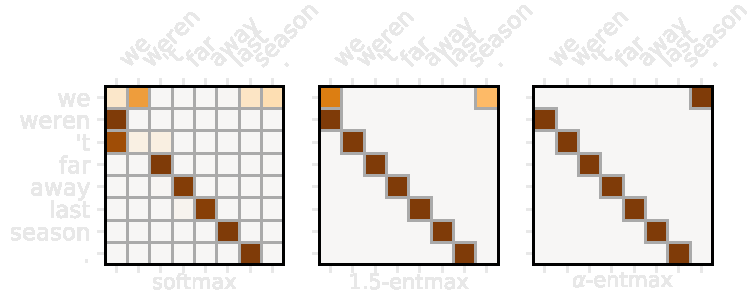
\includegraphics[width=0.9\columnwidth]{figures/head_prev_mybg}\\
    \fontsize{12pt}{15}\selectfont
    This head role was also found in \citet{specialized}! Learned {\color{myDarkYellow}$\alpha = 1.91$}.
    \end{center}

\end{frame}

% \begin{frame}
%     \frametitle{Interrogation-Detecting Head}
%     \vspace{-0.5cm}
%     \begin{center}
%     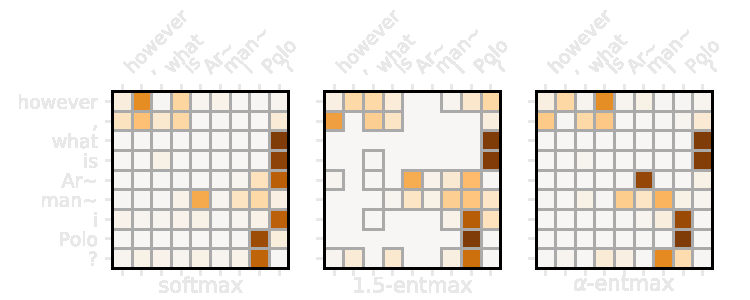
\includegraphics[width=0.9\columnwidth]{figures/head_interro_mybg}\\
%     \fontsize{12pt}{15}\selectfont
%     Learned {\color{myDarkYellow}$\alpha = 1.05$}.
%     \end{center}

% \end{frame}

% \begin{frame}
%     \frametitle{Subword-Merging Head}
%     \vspace{-0.7cm}
%     \begin{columns}[T]
%         \small
%         \begin{column}{.33\textwidth}
%         \vspace{-0.1cm}
%         \centering
%         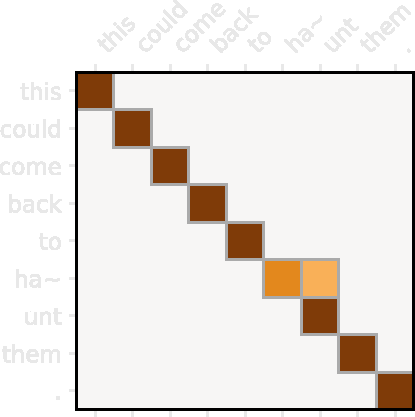
\includegraphics[width=0.9\columnwidth]{figures/bpe4}
%         \end{column}
%         \begin{column}{.33\textwidth}
%         \vspace{-0.2cm}
%         \centering
%         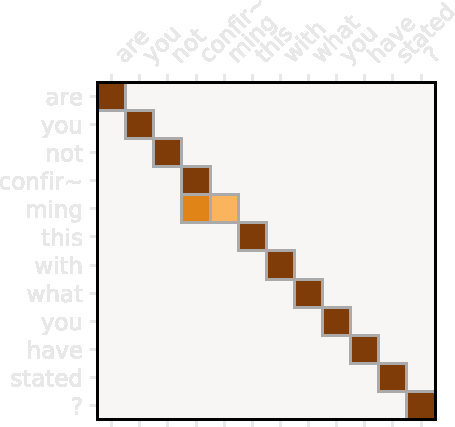
\includegraphics[width=\columnwidth]{figures/bpe3}
%         \end{column}
%         \begin{column}{.33\textwidth}
%         \centering
%         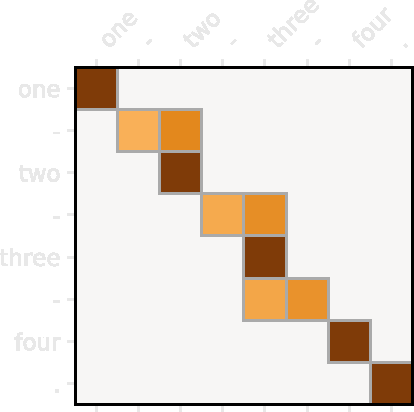
\includegraphics[width=0.9\columnwidth]{figures/bpe2}
%         \end{column}
%         \end{columns}

%         \begin{center}
%             \fontsize{12pt}{15}\selectfont
%             Learned {\color{myDarkYellow}$\alpha = 1.91$}.
%         \end{center}

% \end{frame}

\begin{frame}[fragile]
    \frametitle{Key Takeaways}
  
      \centering\fontsize{14pt}{14}\selectfont%
      Introduce {\color{myDarkYellow} adaptive} sparsity\\
      for Transformers via $\alpha$-entmax with a {\color{myDarkYellow}gradient learnable $\alpha$}.
      %
      %
      \vfill
      %
      %
      \begin{columns}[T]
      \small
      \begin{column}{.33\textwidth}
      \centering
      \uncover<2->{
      \textbf{\emph{adaptive sparsity}}\\[.5\baselineskip]
      \vspace{0.2cm}
      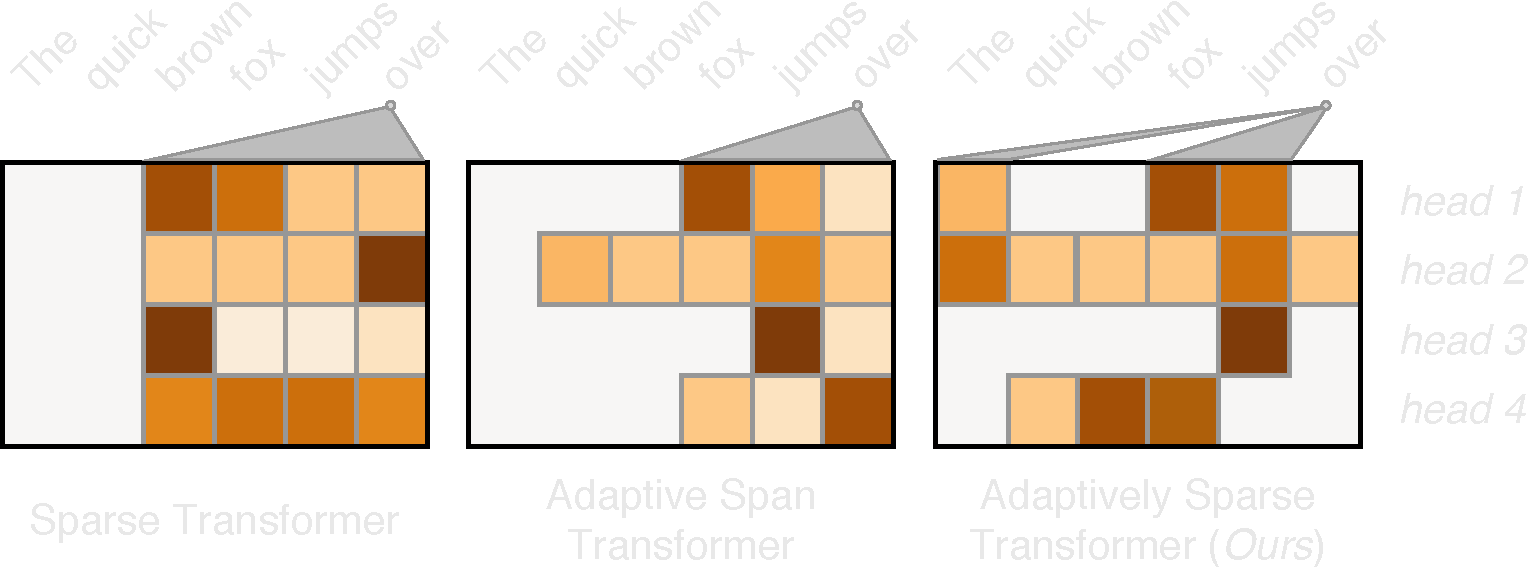
\includegraphics[trim=157mm 17mm 0 0, clip, width=.7\textwidth]{figures/comparison_mybg}}%
      \end{column}
      \begin{column}{.33\textwidth}
      \centering
      \uncover<3->{
      \textbf{\emph{reduced head redundancy}}\\[\baselineskip]}
      \vspace{-0.2cm}
      \begin{tikzpicture}[node distance=1.5ex,font=\scriptsize,scale=0.5, visible on=<3->]
  
          \definecolor{color0}{rgb}{0.12156862745098,0.466666666666667,0.705882352941177}
          \definecolor{color1}{rgb}{1,0.498039215686275,0.0549019607843137}
          \definecolor{color2}{rgb}{0.172549019607843,0.627450980392157,0.172549019607843}
          
          \begin{groupplot}[group style={group size=1 by 1}]
          \nextgroupplot[
          legend cell align={left},
          legend style={
                  nodes={scale=1.1, transform shape}, at={(0.97,0.2)}, anchor=east, draw=white!80.0!black, fill=myfg!30!mybg},
          tick align=outside,
          tick pos=left,
          x grid style={white!69.01960784313725!black},
          xmin=0.5, xmax=6.5,
          xtick = {1, 2, 3, 4, 5, 6},
          xtick style={color=white},
          y grid style={white!69.01960784313725!black},
          ymin=0.1, ymax=0.7,
          ytick = {0.2, 0.4, 0.6},
          ytick style={color=white}
          ]
          \addplot [thick, color0, mark=square*, mark size=3, mark options={solid}]
          table {%
          1 0.38571667343747
          2 0.402429158203537
          3 0.440747738282957
          4 0.359233941813858
          5 0.337470844946825
          6 0.339900884621234
          };
          \addlegendentry{softmax}
          \addplot [thick, color1, mark=*, mark size=3, mark options={solid}]
          table {%
          1 0.378367748537659
          2 0.504354104995477
          3 0.573529792473815
          4 0.525266398541884
          5 0.439669581263257
          6 0.421346772557364
          };
          \addlegendentry{1.5-entmax}
          \addplot [thick, color2, mark=asterisk, mark size=3, mark options={solid}]
          table {%
          1 0.427742934860258
          2 0.484287995253192
          3 0.533714455762104
          4 0.449772918584636
          5 0.3935698561848
          6 0.355665944457941
          };
          \addlegendentry{$\alpha$-entmax}
      \end{groupplot}
      \end{tikzpicture}
      \end{column}
      \begin{column}{.33\textwidth}
      \centering
      \uncover<4->{
      \textbf{\emph{clearer head roles}}\\[\baselineskip]
      \vspace{-0.2cm}
      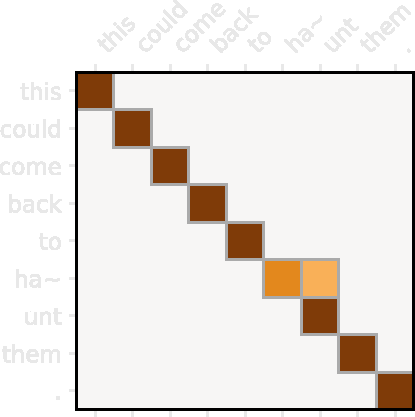
\includegraphics[width=.6\textwidth]{figures/bpe4}}
      \end{column}
      \end{columns}
  
    %   \vfill
  
    %   \centering
    %   {\scriptsize
    %   \color{mygr}
    %   \begin{tabular}{r@{~}l@{\quad}r@{~}l}
    %   \raisebox{-0.7mm}[\height][\depth]{\emoji{githubfg}}& \href{https://github.com/deep-spin/entmax}{\tt github.com/deep-spin/entmax} &
    %   \raisebox{-0.4mm}[\height][\depth]{\emoji{home}}& \href{https://goncalomcorreia.github.io}{\tt goncalomcorreia.github.io}
    %   \end{tabular}}
  
  \end{frame}

\section{Efficient Marginalization of Discrete and Structured Latent Variables via Sparsity}

\begin{frame}
    \frametitle{Latent Variable Models}

    \begin{itemize}
        \uncover<1->{\item[] Latent variable $z$ can be }\uncover<2->{{\color{tGreen} continuous}}\uncover<3->{, {\color{tPeony} discrete}}\uncover<4->{, or {\color{tVividBlue} structured}}
    \end{itemize}
    
    \only<1-2>{\uncover<2>{
    \begin{figure}[hb]
        \centering
        \begin{subfigure}[b]{0.24\columnwidth}
            \centering
            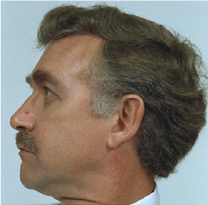
\includegraphics[width=\columnwidth]{figures/face1.png}
        \end{subfigure}
        \hfill
        \begin{subfigure}[b]{0.24\columnwidth}
            \centering
            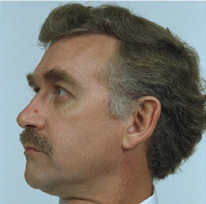
\includegraphics[width=\columnwidth]{figures/face2.png}
        \end{subfigure}
        \hfill
        \begin{subfigure}[b]{0.24\columnwidth}
            \centering
            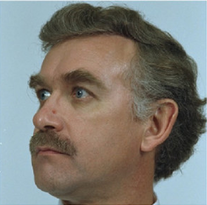
\includegraphics[width=\columnwidth]{figures/face3.png}
        \end{subfigure}
        \hfill
        \begin{subfigure}[b]{0.24\columnwidth}
            \centering
            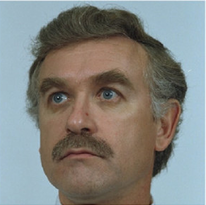
\includegraphics[width=\columnwidth]{figures/face4.png}
        \end{subfigure}
        \caption{Source: \cite{faces}}
        \label{fig:rotation}
    \end{figure}
    }}

    \only<3>{
    \begin{figure}[hb]
        \centering
            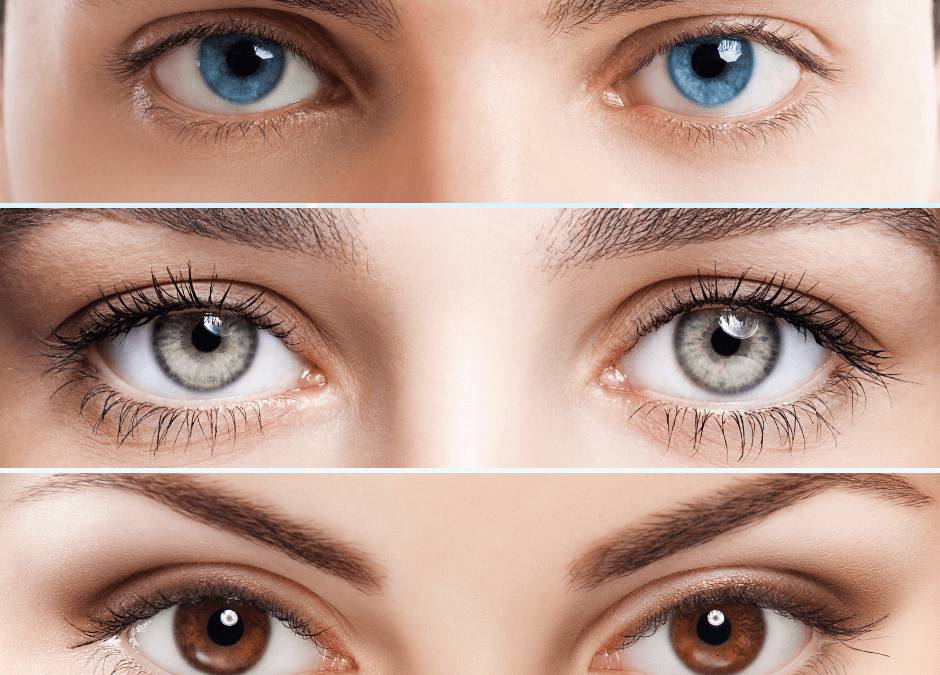
\includegraphics[width=0.5\columnwidth]{figures/eyes.png}
            \caption{Source: \href{https://valleyeyecareaz.com/how-is-your-eye-color-determined/}{valleyeyecareaz.com}}
        \label{fig:eyes}
    \end{figure}
    }

    \only<4>{
    \begin{figure}[hb]
        \centering
            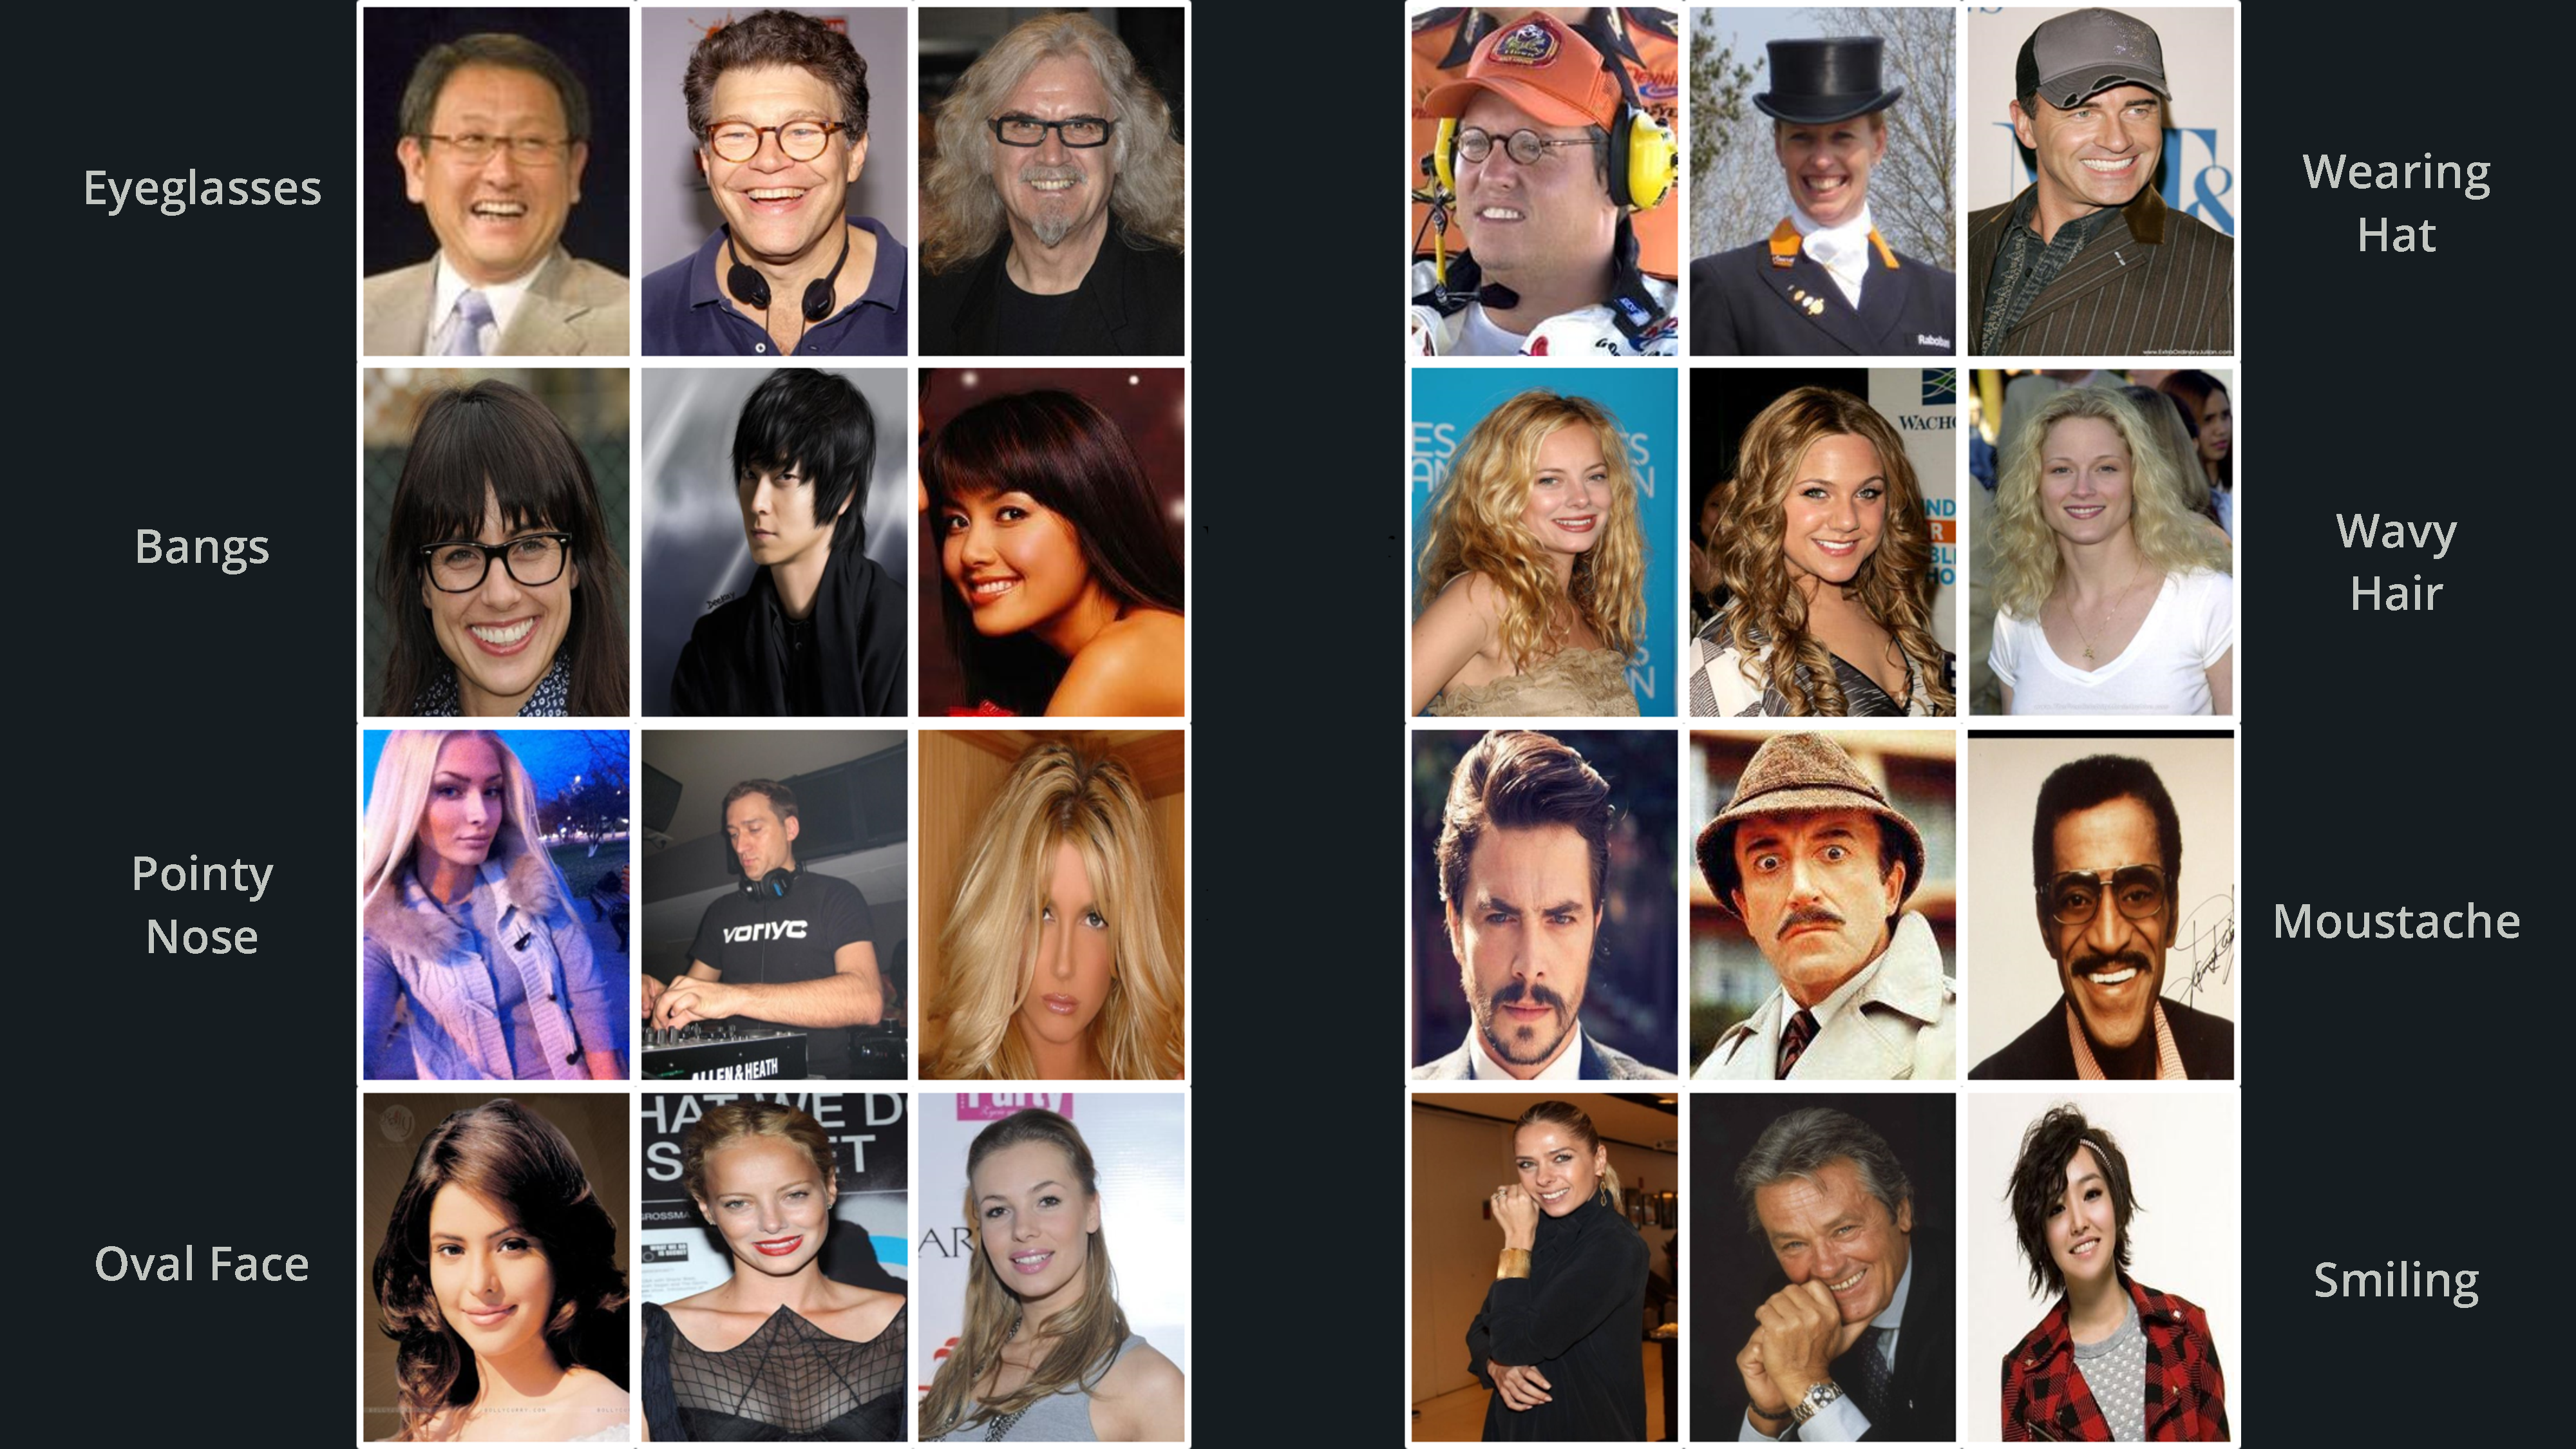
\includegraphics[width=0.6\columnwidth]{figures/celeba_bg.pdf}
            \caption{Source: \cite{liu2015faceattributes}}
        \label{fig:eyes}
    \end{figure}
    }

\end{frame}

\begin{frame}
    \frametitle{Training Discrete or Structured Latent Variable Models}
    \fontsize{12pt}{15}\selectfont

    \begin{columns}
    \hspace{2mm}\vspace{-1cm}\begin{column}{0.7\columnwidth}\vspace{-1cm}
    \begin{itemize}
        \uncover<1->{\item[] Latent variable $z$ can be }\uncover<2->{{\color{tPeony} discrete}}\uncover<3->{ or {\color{tVividBlue} structured}}
    \end{itemize}

    \begin{itemize}
        \uncover<4->{\item[] $\pi(z | x, \theta)$: distribution over possible $z$}
    \end{itemize}

    % besides this, there's also
    \begin{itemize}
        \uncover<7->{\item[] $\ell(x, z; \theta)$: downstream loss: ELBO, Log-Likelihood, (...)}
    \end{itemize}

    \end{column}

    \begin{column}{0.25\columnwidth}
            \vspace{-0.5cm}
            \begin{center}
                \begin{figure}[ht]
                \begin{tikzpicture}
                    % DISCRETE
                    \uncover<2->{\draw[draw=tPink,fill=tPink] (1.4,2) circle (0.2) node[anchor=south, yshift=2mm] {{\visible<5->{\color{tPeony} \small 0.2}}};}
                    \uncover<2->{\draw[draw=tSlateBlue,fill=tSlateBlue] (2,2) circle (0.2) node[anchor=south, yshift=2mm] {{\visible<5->{\color{tPeony} \small 0.6}}};}
                    \uncover<2->{\draw[draw=tGreen,fill=tGreen] (2.6,2) circle (0.2) node[anchor=south, yshift=2mm] {{\visible<5->{\color{tPeony} \small 0.1}}};}

                    % STRUCTURE
                    \uncover<3->{\draw[draw=tSlateBlue,fill=tSlateBlue] (1.4,1) circle (0.2) node[anchor=east, xshift=-2mm] {$[$};}
                    \uncover<3->{\draw[draw=tGreen,fill=tGreen] (2,1) circle (0.2);}
                    \uncover<3->{\draw[draw=tPink,fill=tPink] (2.6,1) circle (0.2)
                        node[anchor=west, xshift=2mm] {$]$}
                        node[anchor=west, xshift=5mm] {{\visible<6->{\color{tVividBlue} \small 0.4}}};}

                    \uncover<3->{\draw[draw=tPink,fill=tPink] (1.4,0.5) circle (0.2) node[anchor=east, xshift=-2mm] {$[$};}
                    \uncover<3->{\draw[draw=tSlateBlue,fill=tSlateBlue] (2,0.5) circle (0.2) node[anchor=north, yshift=-4mm] {\large \bf $\ldots$};}
                    \uncover<3->{\draw[draw=tGreen,fill=tGreen] (2.6,0.5) circle (0.2)
                        node[anchor=west, xshift=2mm] {$]$}
                        node[anchor=west, xshift=5mm] {{\visible<6->{\color{tVividBlue} \small 0.05}}};}

                    \uncover<3->{\draw[draw=tGreen,fill=tGreen] (1.4,-0.5) circle (0.2) node[anchor=east, xshift=-2mm] {$[$};}
                    \uncover<3->{\draw[draw=tSlateBlue,fill=tSlateBlue] (2,-0.5) circle (0.2);}
                    \uncover<3->{\draw[draw=tPink,fill=tPink] (2.6,-0.5) circle (0.2)
                        node[anchor=west, xshift=2mm] {$]$}
                        node[anchor=west, xshift=5mm] {{\visible<6->{\color{tVividBlue} \small 0.3}}};}
                \end{tikzpicture}
                \end{figure}
            \end{center}
    \end{column}
    \end{columns}

    \vspace{-0.5cm}

    \begin{itemize}
        \uncover<8->{\item[] To train, we need to compute the following expectation:}
    \end{itemize}

    \begin{equation*}\label{eq:fit}
        \uncover<9->{\mathcal{L}_{x}(\theta) =
        \sum_{z \in \mathcal Z}
        \pi(z | x, \theta)
        ~\ell(x, z; \theta)}
    \end{equation*}

    \begin{itemize}
        \uncover<10->
        {\item[] If $\mathcal Z$ is
        \only<10>{{\color{tPeony} large}, this sum can get very expensive due to $\ell(x, z; \theta)$!\quad\emoji{oface}}
        \only<11->{{\color{tVividBlue} combinatorial}, this can be intractable to compute!\quad\emoji{oface}\enspace\emoji{oface}\enspace\emoji{oface}}}
    \end{itemize}

\end{frame}

\begin{frame}
    \frametitle{Current Solutions}
    \fontsize{12pt}{15}\selectfont

    \begin{itemize}
        \item[] If $\mathcal Z$ is large, exact gradient computation is prohibitive
    \end{itemize}

    \bigskip

    \begin{itemize}
        \uncover<2->{\item[] One option: SFE (aka REINFORCE) $\rightarrow$ unbiased but high variance}
        \uncover<3->{\item[] Another option: Gumbel-Softmax $\rightarrow$ continuous relaxation, biased estimation}
    \end{itemize}

    \bigskip

    \begin{itemize}
        \uncover<4->{\item[] New option: {\color{tPeony} use sparsity}!\quad\emoji{palms}}
    \end{itemize}

    \begin{itemize}
        \uncover<5->{\item[] no need for sampling $\rightarrow$ no variance}
        \uncover<6->{\item[] no relaxation into the continuous space}
    \end{itemize}
\end{frame}

\begin{frame}
    \frametitle{Taking a step back...}
    \fontsize{12pt}{15}\selectfont
    \begin{itemize}
        \item[] Does the expectation over possible $z$ need to be expensive?
    \end{itemize}

    \begin{align*}\label{eq:fit}
        \uncover<2->{\mathcal{L}_{x}(\theta) &=
        \sum_{z \in \mathcal Z}
        \pi(z | x, \theta)~\ell(x, z; \theta) \\&=
        \pi(z_1 | x, \theta)~\ell(x, z_1; \theta) + \pi(z_2 | x, \theta)~\ell(x, z_2; \theta) + \ldots \\&+ \pi(z_{\mathrlap{i}\hphantom{1}} | x, \theta)~\ell(x, z_{\mathrlap{i}\hphantom{1}}; \theta) + \ldots + \pi(z_N | x, \theta)~\ell(x, z_N; \theta)
        }
    \end{align*}

    % \begin{itemize}
    %     \uncover<3->{\item[] If components of $\pi(z | x, \theta)$ were exactly $0$, we could skip lots of computations!}
    % \end{itemize}

    \begin{itemize}
        \uncover<3->{\item[] Usually we normalize $\pi$ with $\text{softmax} \propto \exp(s) \Rightarrow \pi(z_{\mathrlap{i}\hphantom{1}} | x, \theta)>0$}
    \end{itemize}
\end{frame}

\begin{frame}
    \frametitle{Sparse normalizers}
    \fontsize{12pt}{10}\selectfont
    \cornercite[north east]{sparsemax, sparsemap}
    \begin{itemize}
        \item[] We use {\color{tPeony} sparsemax}, {\color{tVividBlue} top-$k$ sparsemax} and {\color{tVividBlue} SparseMAP} to allow efficient marginalization
    \end{itemize}

    \begin{itemize}
        \uncover<2->{\item[] These functions are able to assign {\bf probabilities of exactly zero}!}
    \end{itemize}

    \begin{align*}
        \uncover<3->{\mathcal{L}_{x}(\theta) &=
        \sum_{z \in \mathcal Z}
        \pi(z | x, \theta)~\ell(x, z; \theta) \\&=
        \pi(z_1 | x, \theta)~\ell(x, z_1; \theta) + \alt<3>{\underbrace{\pi(z_2 | x, \theta)}_{=0}~\ell(x, z_2; \theta)}{\cancel{\underbrace{\pi(z_2 | x, \theta)}_{=0}~\ell(x, z_2; \theta)}} + \ldots \\&+
        \pi(z_{\mathrlap{i}\hphantom{1}} | x, \theta)~\ell(x, z_{\mathrlap{i}\hphantom{1}}; \theta) + \ldots + \alt<3>{\underbrace{\pi(z_N | x, \theta)}_{=0}~\ell(x, z_N; \theta)}{\cancel{\underbrace{\pi(z_N | x, \theta)}_{=0}~\ell(x, z_N; \theta)}}
        }
    \end{align*}

    \begin{itemize}
        \uncover<4->{\item[] No need for computing $\ell(x, z; \theta)$ for all $z \in \mathcal Z$!}
    \end{itemize}
\end{frame}

% \begin{frame}
%     \frametitle{Semi-Supervised VAE}%\cornerciteme{sparsemarg}

%     \newcommand*\parcolor{myfg}
%     \newcommand*\clfcolor{myfg}
%     \newcommand*\colParseZero{mybg}
%     \newcommand*\colParseNonz{mybg}
%     \renewcommand*\parcolor{tPeony}
%     \renewcommand*\clfcolor{tYellow}

%     \begin{align*}
%         \mathcal{L}_{x}(\theta) &=
%             \tikzmark{sum}\sum_{z \in \mathcal{Z}}
%             \textcolor{\parcolor}{\pi\tikzmark{parp}(z | x)}~
%             \textcolor{\clfcolor}{\ell\tikzmark{clfp}(x, z)}\\
%             &= \mathbb{E}_{z \sim \textcolor{\parcolor}{\pi(z | x)}}~%
%             \textcolor{\clfcolor}{\ell(x, z)}
%     \end{align*}

%     \vspace{\baselineskip}
%     \begin{itemize}
%     \item<1-> Semi-Supervised VAE on MNIST: $z$ is one of 10 categories
%     \item<4-> Train this with 10\% labeled data
%     \end{itemize}
%     \begin{tikzpicture}[%
%         remember picture,
%         overlay,
%         expl/.style={font=\small}]
%     \uncover<2->{
%         \node[expl,anchor=north east] (explpar)
%             at ($(current page.north east) - (.5, 2.0)$)
%             {Gaussian VAE};
%         \path (explpar.west) edge[->,very thick,bend right] ([yshift=2.0ex]{pic cs:clfp});
%     }
%     %
%     \uncover<3->{
%         \node[expl,anchor=north west,align=left] (explsum)
%             at ($(current page.west) + (.5, 1.5)$)
%             {sum over \\ the 10 digits};
%         \path (explsum.east) edge[->,very thick,bend left] ([yshift=2.5ex]{pic cs:sum});
%     }
%     \uncover<2->{
%         \node[expl,anchor=north east,align=right] (explscore)
%             at ($(current page.north east) - (.5, 3.5)$)
%             {classification network};
%         \path (explscore.south west) edge[->,very thick,bend left] ([yshift=-1.0ex]{pic cs:parp});
%     }
%     \end{tikzpicture}
% \end{frame}

% \begin{frame}
%     \frametitle{Semi-Supervised VAE}
%     \begin{columns}[T]
%     \begin{column}{.53\textwidth}
%         \centering\small%
%         \begin{tabular}{lrr}
%             \toprule
%             Method &
%             Accuracy (\%)
%             & Dec. calls\\
%             \midrule
%         \multicolumn{3}{l}{\emph{Monte Carlo}} \\
%             SFE
%             & $94.75${\tiny\color{gray}$\pm .002$} & $1$ \\
%             SFE$+$
%             & $96.53${\tiny\color{gray}$\pm .001$}  & $2$  \\
%             NVIL
%             & $96.01${\tiny\color{gray}$\pm .002$}  & $1$  \\
%             Gumbel
%             & $95.46${\tiny\color{gray}$\pm .001$}  & $1$  \\
%             \midrule
%         \multicolumn{3}{l}{\emph{Marginalization}} \\
%             Dense
%             & $96.93${\tiny\color{gray}$\pm .001$}  & $10$  \\
%             \only<2->{\textcolor{tPeony}{Sparse}
%             & $96.87${\tiny\color{gray}$\pm .001$}  & $1.01${\tiny\color{gray}$\pm 0.01$}}  \\
%             \bottomrule
%             \end{tabular}
%     \end{column}
%     \begin{column}{.47\textwidth}
%         \centering%
%         \onslide<3->{
%         % This file was created by tikzplotlib v0.9.4.
\small
\begin{tikzpicture}

\definecolor{color0}{rgb}{0.894117647058824,0.101960784313725,0.109803921568627}
\definecolor{color1}{rgb}{1,0.498039215686275,0}
\definecolor{color2}{rgb}{0.968627450980392,0.505882352941176,0.749019607843137}
\definecolor{color3}{rgb}{0.215686274509804,0.494117647058824,0.72156862745098}
\definecolor{color4}{rgb}{0.870588235294118,0.870588235294118,0}

\begin{axis}[
scale=.75,
legend cell align={left},
legend style={fill opacity=0.1, draw opacity=1, text opacity=1},
tick align=outside,
tick pos=left,
x grid style={white!69.0196078431373!black},
xlabel={Epoch},
xmin=1, xmax=202,
xtick style={color=black},
y grid style={white!69.0196078431373!black},
ylabel={Negative ELBO},
ymin=97.1, ymax=105.5,
ytick style={color=black}
]
\path [draw=color0, line width=1pt]
(axis cs:0,110.571628222803)
--(axis cs:0,110.616042675635);

\path [draw=color0, line width=1pt]
(axis cs:5,105.62209213224)
--(axis cs:5,105.704893036217);

\path [draw=color0, line width=1pt]
(axis cs:10,104.289450185493)
--(axis cs:10,104.356994516656);

\path [draw=color0, line width=1pt]
(axis cs:15,103.407209298477)
--(axis cs:15,103.476579764023);

\path [draw=color0, line width=1pt]
(axis cs:20,102.773344218468)
--(axis cs:20,102.825509846474);

\path [draw=color0, line width=1pt]
(axis cs:25,102.213106343832)
--(axis cs:25,102.282459452066);

\path [draw=color0, line width=1pt]
(axis cs:30,101.725467036023)
--(axis cs:30,101.820451237903);

\path [draw=color0, line width=1pt]
(axis cs:35,101.245988632048)
--(axis cs:35,101.334083389436);

\path [draw=color0, line width=1pt]
(axis cs:40,100.909448112661)
--(axis cs:40,100.97308362562);

\path [draw=color0, line width=1pt]
(axis cs:45,100.543817511853)
--(axis cs:45,100.626635369007);

\path [draw=color0, line width=1pt]
(axis cs:50,100.299712409677)
--(axis cs:50,100.380463371573);

\path [draw=color0, line width=1pt]
(axis cs:55,99.9914284050014)
--(axis cs:55,100.074857300565);

\path [draw=color0, line width=1pt]
(axis cs:60,99.9003536552268)
--(axis cs:60,100.007995954148);

\path [draw=color0, line width=1pt]
(axis cs:65,99.704677941787)
--(axis cs:65,99.7719318604591);

\path [draw=color0, line width=1pt]
(axis cs:70,99.512591227806)
--(axis cs:70,99.6056003005144);

\path [draw=color0, line width=1pt]
(axis cs:75,99.2968394860584)
--(axis cs:75,99.3603535071057);

\path [draw=color0, line width=1pt]
(axis cs:80,99.1895523660352)
--(axis cs:80,99.3006438619921);

\path [draw=color0, line width=1pt]
(axis cs:85,99.0947624008693)
--(axis cs:85,99.1854026992284);

\path [draw=color0, line width=1pt]
(axis cs:90,98.9419574019052)
--(axis cs:90,99.0291546586417);

\path [draw=color0, line width=1pt]
(axis cs:95,98.7685936844909)
--(axis cs:95,98.8469992720521);

\path [draw=color0, line width=1pt]
(axis cs:100,98.6924243915877)
--(axis cs:100,98.7649715434708);

\path [draw=color0, line width=1pt]
(axis cs:105,98.6493410445112)
--(axis cs:105,98.7355893754106);

\path [draw=color0, line width=1pt]
(axis cs:110,98.4847570378102)
--(axis cs:110,98.5481546443187);

\path [draw=color0, line width=1pt]
(axis cs:115,98.3900102720628)
--(axis cs:115,98.4639402284255);

\path [draw=color0, line width=1pt]
(axis cs:120,98.4279693596278)
--(axis cs:120,98.5433822639073);

\path [draw=color0, line width=1pt]
(axis cs:125,98.2681371217175)
--(axis cs:125,98.3506113524036);

\path [draw=color0, line width=1pt]
(axis cs:130,98.2755771208057)
--(axis cs:130,98.3637051057568);

\path [draw=color0, line width=1pt]
(axis cs:135,98.1519624650895)
--(axis cs:135,98.244399839598);

\path [draw=color0, line width=1pt]
(axis cs:140,98.1250063491776)
--(axis cs:140,98.2095242904708);

\path [draw=color0, line width=1pt]
(axis cs:145,97.9583158375388)
--(axis cs:145,98.0694994090433);

\path [draw=color0, line width=1pt]
(axis cs:150,98.0437309578043)
--(axis cs:150,98.1430503532309);

\path [draw=color0, line width=1pt]
(axis cs:155,97.9080906432997)
--(axis cs:155,98.0325358825793);

\path [draw=color0, line width=1pt]
(axis cs:160,97.9438041674736)
--(axis cs:160,97.9982872021553);

\path [draw=color0, line width=1pt]
(axis cs:165,97.7717692124589)
--(axis cs:165,97.8538380873458);

\path [draw=color0, line width=1pt]
(axis cs:170,97.7947733818513)
--(axis cs:170,97.9104039252776);

\path [draw=color0, line width=1pt]
(axis cs:175,97.7514530083922)
--(axis cs:175,97.8663829901429);

\path [draw=color0, line width=1pt]
(axis cs:180,97.7297998759255)
--(axis cs:180,97.804909291555);

\path [draw=color0, line width=1pt]
(axis cs:185,97.6381521365036)
--(axis cs:185,97.7025918820511);

\path [draw=color0, line width=1pt]
(axis cs:190,97.6893112699308)
--(axis cs:190,97.8114165743075);

\path [draw=color0, line width=1pt]
(axis cs:195,97.530511048186)
--(axis cs:195,97.6161030265211);

\path [draw=color0, line width=1pt]
(axis cs:200,97.6454695308675)
--(axis cs:200,97.7513017093669);

\path [draw=color1, thick]
(axis cs:0,110.627656081213)
--(axis cs:0,110.677801987635);

\path [draw=color1, thick]
(axis cs:5,105.706752241274)
--(axis cs:5,105.865315019468);

\path [draw=color1, thick]
(axis cs:10,104.251092751157)
--(axis cs:10,104.39130837189);

\path [draw=color1, thick]
(axis cs:15,103.02386310639)
--(axis cs:15,103.129296988825);

\path [draw=color1, thick]
(axis cs:20,102.185802869572)
--(axis cs:20,102.311458177791);

\path [draw=color1, thick]
(axis cs:25,101.498045278342)
--(axis cs:25,101.599491953103);

\path [draw=color1, thick]
(axis cs:30,101.074134287995)
--(axis cs:30,101.195169606048);

\path [draw=color1, thick]
(axis cs:35,100.688277085196)
--(axis cs:35,100.794839064706);

\path [draw=color1, thick]
(axis cs:40,100.470196032671)
--(axis cs:40,100.584731030317);

\path [draw=color1, thick]
(axis cs:45,100.114440390114)
--(axis cs:45,100.257237771508);

\path [draw=color1, thick]
(axis cs:50,99.8929637508349)
--(axis cs:50,99.9790409488721);

\path [draw=color1, thick]
(axis cs:55,99.4751854380556)
--(axis cs:55,99.6703162709288);

\path [draw=color1, thick]
(axis cs:60,99.4392706157917)
--(axis cs:60,99.6078973529582);

\path [draw=color1, thick]
(axis cs:65,99.2057001296773)
--(axis cs:65,99.3453481491313);

\path [draw=color1, thick]
(axis cs:70,99.139523129024)
--(axis cs:70,99.2743074373822);

\path [draw=color1, thick]
(axis cs:75,99.0585529362254)
--(axis cs:75,99.1688610042043);

\path [draw=color1, thick]
(axis cs:80,98.863532244795)
--(axis cs:80,98.9907447937792);

\path [draw=color1, thick]
(axis cs:85,98.6890531083094)
--(axis cs:85,98.791636894132);

\path [draw=color1, thick]
(axis cs:90,98.6046054723124)
--(axis cs:90,98.7568752405782);

\path [draw=color1, thick]
(axis cs:95,98.5015275966912)
--(axis cs:95,98.6355482089728);

\path [draw=color1, thick]
(axis cs:100,98.5031524382435)
--(axis cs:100,98.6100830353893);

\path [draw=color1, thick]
(axis cs:105,98.4936773624417)
--(axis cs:105,98.6237222347263);

\path [draw=color1, thick]
(axis cs:110,98.3101249716939)
--(axis cs:110,98.4445198036967);

\path [draw=color1, thick]
(axis cs:115,98.427620263025)
--(axis cs:115,98.5260891485961);

\path [draw=color1, thick]
(axis cs:120,98.2365748731903)
--(axis cs:120,98.3342777879425);

\path [draw=color1, thick]
(axis cs:125,98.2255084713109)
--(axis cs:125,98.38844111365);

\path [draw=color1, thick]
(axis cs:130,98.1163595550203)
--(axis cs:130,98.2660211212493);

\path [draw=color1, thick]
(axis cs:135,98.0937488614553)
--(axis cs:135,98.2127208651072);

\path [draw=color1, thick]
(axis cs:140,98.0585679595026)
--(axis cs:140,98.1632795746771);

\path [draw=color1, thick]
(axis cs:145,98.1005616053344)
--(axis cs:145,98.2021132603883);

\path [draw=color1, thick]
(axis cs:150,98.029635259175)
--(axis cs:150,98.1676334175828);

\path [draw=color1, thick]
(axis cs:155,98.0933789691696)
--(axis cs:155,98.1758226909867);

\path [draw=color1, thick]
(axis cs:160,97.9562209316475)
--(axis cs:160,98.0729889682549);

\path [draw=color1, thick]
(axis cs:165,97.949017347317)
--(axis cs:165,98.0935470447728);

\path [draw=color1, thick]
(axis cs:170,97.8620924517951)
--(axis cs:170,97.9806428387322);

\path [draw=color1, thick]
(axis cs:175,97.9098973693818)
--(axis cs:175,98.0343851623565);

\path [draw=color1, thick]
(axis cs:180,97.8642887851381)
--(axis cs:180,98.0409861782408);

\path [draw=color1, thick]
(axis cs:185,97.766666124376)
--(axis cs:185,97.9967158336318);

\path [draw=color1, thick]
(axis cs:190,97.788889657506)
--(axis cs:190,97.8705555329237);

\path [draw=color1, thick]
(axis cs:195,97.7695971257876)
--(axis cs:195,97.8705502741148);

\path [draw=color1, thick]
(axis cs:200,97.676539048256)
--(axis cs:200,97.8900106343612);

\path [draw=color2, thick]
(axis cs:0,110.667671743089)
--(axis cs:0,110.722681650465);

\path [draw=color2, thick]
(axis cs:5,106.483563798014)
--(axis cs:5,106.755126387533);

\path [draw=color2, thick]
(axis cs:10,105.265325161184)
--(axis cs:10,105.615572360788);

\path [draw=color2, thick]
(axis cs:15,104.528087390467)
--(axis cs:15,104.730024181799);

\path [draw=color2, thick]
(axis cs:20,103.768548703352)
--(axis cs:20,103.906315493426);

\path [draw=color2, thick]
(axis cs:25,103.117035642729)
--(axis cs:25,103.338207277193);

\path [draw=color2, thick]
(axis cs:30,102.790858085322)
--(axis cs:30,102.949431221319);

\path [draw=color2, thick]
(axis cs:35,102.420181417919)
--(axis cs:35,102.692468118214);

\path [draw=color2, thick]
(axis cs:40,101.953505979879)
--(axis cs:40,102.11779834141);

\path [draw=color2, thick]
(axis cs:45,101.605904790239)
--(axis cs:45,101.75691717021);

\path [draw=color2, thick]
(axis cs:50,101.470575734144)
--(axis cs:50,101.61874616527);

\path [draw=color2, thick]
(axis cs:55,101.197271375808)
--(axis cs:55,101.416739244309);

\path [draw=color2, thick]
(axis cs:60,100.910259467554)
--(axis cs:60,101.06691033225);

\path [draw=color2, thick]
(axis cs:65,100.811883301745)
--(axis cs:65,101.000802855481);

\path [draw=color2, thick]
(axis cs:70,100.628725831965)
--(axis cs:70,100.885245115301);

\path [draw=color2, thick]
(axis cs:75,100.324332760492)
--(axis cs:75,100.442026187261);

\path [draw=color2, thick]
(axis cs:80,100.178942312571)
--(axis cs:80,100.475639901784);

\path [draw=color2, thick]
(axis cs:85,99.9694360453458)
--(axis cs:85,100.165645436588);

\path [draw=color2, thick]
(axis cs:90,99.7062381923905)
--(axis cs:90,99.9938823520431);

\path [draw=color2, thick]
(axis cs:95,99.782874624705)
--(axis cs:95,99.8487354827169);

\path [draw=color2, thick]
(axis cs:100,99.6613457276373)
--(axis cs:100,99.7565757201167);

\path [draw=color2, thick]
(axis cs:105,99.4611038629233)
--(axis cs:105,99.5586761053385);

\path [draw=color2, thick]
(axis cs:110,99.4817789142452)
--(axis cs:110,99.6602132732548);

\path [draw=color2, thick]
(axis cs:115,99.3468294377173)
--(axis cs:115,99.4159482722436);

\path [draw=color2, thick]
(axis cs:120,99.141580926534)
--(axis cs:120,99.271195257548);

\path [draw=color2, thick]
(axis cs:125,99.1192806472576)
--(axis cs:125,99.2834537277424);

\path [draw=color2, thick]
(axis cs:130,99.0235558578023)
--(axis cs:130,99.1700354507914);

\path [draw=color2, thick]
(axis cs:135,99.1761870048272)
--(axis cs:135,99.532272467829);

\path [draw=color2, thick]
(axis cs:140,99.1153352177682)
--(axis cs:140,99.2472807490287);

\path [draw=color2, thick]
(axis cs:145,98.7532872367982)
--(axis cs:145,98.8955485175963);

\path [draw=color2, thick]
(axis cs:150,98.8283402895275)
--(axis cs:150,98.9566206479725);

\path [draw=color2, thick]
(axis cs:155,98.768272445518)
--(axis cs:155,98.8687789460836);

\path [draw=color2, thick]
(axis cs:160,98.8125847348663)
--(axis cs:160,98.9838111391571);

\path [draw=color2, thick]
(axis cs:165,98.5870355780569)
--(axis cs:165,98.7299962822946);

\path [draw=color2, thick]
(axis cs:170,98.5641170271013)
--(axis cs:170,98.7153095476057);

\path [draw=color2, thick]
(axis cs:175,98.5214131010244)
--(axis cs:175,98.702083908253);

\path [draw=color2, thick]
(axis cs:180,98.3888573706301)
--(axis cs:180,98.488860219702);

\path [draw=color2, thick]
(axis cs:185,98.3901603236432)
--(axis cs:185,98.620610855556);

\path [draw=color2, thick]
(axis cs:190,98.4326878189535)
--(axis cs:190,98.6290248275309);

\path [draw=color2, thick]
(axis cs:195,98.3281897838033)
--(axis cs:195,98.5063866322123);

\path [draw=color2, thick]
(axis cs:200,98.3254687617908)
--(axis cs:200,98.4676388431897);

\path [draw=color3, thick]
(axis cs:0,110.602628549784)
--(axis cs:0,110.654276052266);

\path [draw=color3, thick]
(axis cs:5,105.976421191421)
--(axis cs:5,106.086629650864);

\path [draw=color3, thick]
(axis cs:10,104.686016970886)
--(axis cs:10,104.733898800599);

\path [draw=color3, thick]
(axis cs:15,103.722053944156)
--(axis cs:15,103.865365184262);

\path [draw=color3, thick]
(axis cs:20,103.028494114149)
--(axis cs:20,103.116822963487);

\path [draw=color3, thick]
(axis cs:25,102.6033735088)
--(axis cs:25,102.73937246288);

\path [draw=color3, thick]
(axis cs:30,101.982135306812)
--(axis cs:30,102.062316597485);

\path [draw=color3, thick]
(axis cs:35,101.56680058494)
--(axis cs:35,101.653621778342);

\path [draw=color3, thick]
(axis cs:40,101.228760366328)
--(axis cs:40,101.308081979864);

\path [draw=color3, thick]
(axis cs:45,100.91559693553)
--(axis cs:45,101.09211790822);

\path [draw=color3, thick]
(axis cs:50,100.715529800361)
--(axis cs:50,100.781035446221);

\path [draw=color3, thick]
(axis cs:55,100.284129784015)
--(axis cs:55,100.401266028973);

\path [draw=color3, thick]
(axis cs:60,100.136854336586)
--(axis cs:60,100.240103366051);

\path [draw=color3, thick]
(axis cs:65,99.8551212918418)
--(axis cs:65,99.9795039522988);

\path [draw=color3, thick]
(axis cs:70,99.7252302427781)
--(axis cs:70,99.8387315492141);

\path [draw=color3, thick]
(axis cs:75,99.5236912911197)
--(axis cs:75,99.6395121390561);

\path [draw=color3, thick]
(axis cs:80,99.4197217550092)
--(axis cs:80,99.5033083353228);

\path [draw=color3, thick]
(axis cs:85,99.3302764392952)
--(axis cs:85,99.4162308238884);

\path [draw=color3, thick]
(axis cs:90,99.1285783522856)
--(axis cs:90,99.1683592087495);

\path [draw=color3, thick]
(axis cs:95,98.9709728146841)
--(axis cs:95,99.0789615725229);

\path [draw=color3, thick]
(axis cs:100,98.8787928184983)
--(axis cs:100,99.0089269080642);

\path [draw=color3, thick]
(axis cs:105,98.8716916737113)
--(axis cs:105,99.0200563731637);

\path [draw=color3, thick]
(axis cs:110,98.7279148782457)
--(axis cs:110,98.8484721456801);

\path [draw=color3, thick]
(axis cs:115,98.6767164317005)
--(axis cs:115,98.7957170399792);

\path [draw=color3, thick]
(axis cs:120,98.5780803608091)
--(axis cs:120,98.6203907085269);

\path [draw=color3, thick]
(axis cs:125,98.4521045701371)
--(axis cs:125,98.5314693434371);

\path [draw=color3, thick]
(axis cs:130,98.3776252768865)
--(axis cs:130,98.4630714394221);

\path [draw=color3, thick]
(axis cs:135,98.348839879622)
--(axis cs:135,98.4589039558272);

\path [draw=color3, thick]
(axis cs:140,98.3020782930936)
--(axis cs:140,98.3743255155002);

\path [draw=color3, thick]
(axis cs:145,98.2389102090793)
--(axis cs:145,98.3121029745145);

\path [draw=color3, thick]
(axis cs:150,98.1700772251234)
--(axis cs:150,98.2461810146227);

\path [draw=color3, thick]
(axis cs:155,98.0599698152065)
--(axis cs:155,98.1876009855747);

\path [draw=color3, thick]
(axis cs:160,98.0501097252529)
--(axis cs:160,98.1519822547276);

\path [draw=color3, thick]
(axis cs:165,97.9869192373277)
--(axis cs:165,98.1074411142348);

\path [draw=color3, thick]
(axis cs:170,97.9562103379446)
--(axis cs:170,98.054098499946);

\path [draw=color3, thick]
(axis cs:175,97.8537923449074)
--(axis cs:175,97.9198068982566);

\path [draw=color3, thick]
(axis cs:180,97.7835440487471)
--(axis cs:180,97.8533425479326);

\path [draw=color3, thick]
(axis cs:185,97.7571509252569)
--(axis cs:185,97.8370385278681);

\path [draw=color3, thick]
(axis cs:190,97.6644307218972)
--(axis cs:190,97.7558863557395);

\path [draw=color3, thick]
(axis cs:195,97.8125477291052)
--(axis cs:195,97.8993236087854);

\path [draw=color3, thick]
(axis cs:200,97.6539407705038)
--(axis cs:200,97.7391317392618);

\path [draw=color4, thick]
(axis cs:0,109.115286948018)
--(axis cs:0,109.381600259013);

\path [draw=color4, thick]
(axis cs:5,106.282004510241)
--(axis cs:5,106.442658270521);

\path [draw=color4, thick]
(axis cs:10,104.396784651101)
--(axis cs:10,104.604474198997);

\path [draw=color4, thick]
(axis cs:15,103.323337914808)
--(axis cs:15,103.482654211657);

\path [draw=color4, thick]
(axis cs:20,102.778455356846)
--(axis cs:20,103.020767970791);

\path [draw=color4, thick]
(axis cs:25,102.055643913527)
--(axis cs:25,102.23702271245);

\path [draw=color4, thick]
(axis cs:30,101.529721481467)
--(axis cs:30,101.638959853983);

\path [draw=color4, thick]
(axis cs:35,101.134941232361)
--(axis cs:35,101.228889334045);

\path [draw=color4, thick]
(axis cs:40,100.906734618429)
--(axis cs:40,101.146105042215);

\path [draw=color4, thick]
(axis cs:45,100.697209372744)
--(axis cs:45,100.824752602354);

\path [draw=color4, thick]
(axis cs:50,100.353978259345)
--(axis cs:50,100.619825451592);

\path [draw=color4, thick]
(axis cs:55,100.084291283199)
--(axis cs:55,100.24559305518);

\path [draw=color4, thick]
(axis cs:60,100.010707402261)
--(axis cs:60,100.119865107505);

\path [draw=color4, thick]
(axis cs:65,99.7864048943775)
--(axis cs:65,99.9255106940014);

\path [draw=color4, thick]
(axis cs:70,99.631284648257)
--(axis cs:70,99.7560169874852);

\path [draw=color4, thick]
(axis cs:75,99.4452606980236)
--(axis cs:75,99.624603193578);

\path [draw=color4, thick]
(axis cs:80,99.3618639961725)
--(axis cs:80,99.4920193656439);

\path [draw=color4, thick]
(axis cs:85,99.2837623633726)
--(axis cs:85,99.3978050194399);

\path [draw=color4, thick]
(axis cs:90,99.266347190475)
--(axis cs:90,99.3817576679235);

\path [draw=color4, thick]
(axis cs:95,99.3123228170201)
--(axis cs:95,99.660885801144);

\path [draw=color4, thick]
(axis cs:100,99.0990519167043)
--(axis cs:100,99.2413808225535);

\path [draw=color4, thick]
(axis cs:105,98.8874418897035)
--(axis cs:105,99.0510957079527);

\path [draw=color4, thick]
(axis cs:110,98.975193322023)
--(axis cs:110,99.2649327155746);

\path [draw=color4, thick]
(axis cs:115,98.8336393432915)
--(axis cs:115,99.0471651000678);

\path [draw=color4, thick]
(axis cs:120,98.8308258199566)
--(axis cs:120,98.9343551492817);

\path [draw=color4, thick]
(axis cs:125,98.656977400232)
--(axis cs:125,98.7910816817992);

\path [draw=color4, thick]
(axis cs:130,98.6945838969624)
--(axis cs:130,98.845497890147);

\path [draw=color4, thick]
(axis cs:135,98.6141177603053)
--(axis cs:135,98.7381649545384);

\path [draw=color4, thick]
(axis cs:140,98.5875804361404)
--(axis cs:140,98.7294895711839);

\path [draw=color4, thick]
(axis cs:145,98.6315291825926)
--(axis cs:145,98.944827323755);

\path [draw=color4, thick]
(axis cs:150,98.5094485836863)
--(axis cs:150,98.6495495242238);

\path [draw=color4, thick]
(axis cs:155,98.3895212745971)
--(axis cs:155,98.5292638206178);

\path [draw=color4, thick]
(axis cs:160,98.2698468425989)
--(axis cs:160,98.4126009723425);

\path [draw=color4, thick]
(axis cs:165,98.3838028476987)
--(axis cs:165,98.5055968715395);

\path [draw=color4, thick]
(axis cs:170,98.2593796537036)
--(axis cs:170,98.3188368990307);

\path [draw=color4, thick]
(axis cs:175,98.5055199805482)
--(axis cs:175,98.6556677635925);

\path [draw=color4, thick]
(axis cs:180,98.2703711104053)
--(axis cs:180,98.403257124458);

\path [draw=color4, thick]
(axis cs:185,98.1379741875829)
--(axis cs:185,98.2555164130031);

\path [draw=color4, thick]
(axis cs:190,98.1838837762334)
--(axis cs:190,98.3041319708369);

\path [draw=color4, thick]
(axis cs:195,98.0923628934146)
--(axis cs:195,98.204795920062);

\path [draw=color4, thick]
(axis cs:200,98.1158716660487)
--(axis cs:200,98.3141988295567);

\path [draw=white!60!black, thick]
(axis cs:0,110.590080177886)
--(axis cs:0,110.625547873871);

\path [draw=white!60!black, thick]
(axis cs:5,105.789744869155)
--(axis cs:5,105.860650333482);

\path [draw=white!60!black, thick]
(axis cs:10,104.306409792426)
--(axis cs:10,104.455569882867);

\path [draw=white!60!black, thick]
(axis cs:15,103.193854098826)
--(axis cs:15,103.300857204885);

\path [draw=white!60!black, thick]
(axis cs:20,102.333934668303)
--(axis cs:20,102.475356408357);

\path [draw=white!60!black, thick]
(axis cs:25,101.853913202521)
--(axis cs:25,101.955892095331);

\path [draw=white!60!black, thick]
(axis cs:30,101.327375788094)
--(axis cs:30,101.43849487841);

\path [draw=white!60!black, thick]
(axis cs:35,100.895046297489)
--(axis cs:35,101.059007962764);

\path [draw=white!60!black, thick]
(axis cs:40,100.721416148737)
--(axis cs:40,100.852466907903);

\path [draw=white!60!black, thick]
(axis cs:45,100.426625423738)
--(axis cs:45,100.555039615324);

\path [draw=white!60!black, thick]
(axis cs:50,100.14122325845)
--(axis cs:50,100.277958565281);

\path [draw=white!60!black, thick]
(axis cs:55,99.8386719808062)
--(axis cs:55,99.9528914347212);

\path [draw=white!60!black, thick]
(axis cs:60,99.6445181644106)
--(axis cs:60,99.7823418819761);

\path [draw=white!60!black, thick]
(axis cs:65,99.5608438090816)
--(axis cs:65,99.7018881245121);

\path [draw=white!60!black, thick]
(axis cs:70,99.4431362586879)
--(axis cs:70,99.5257480186559);

\path [draw=white!60!black, thick]
(axis cs:75,99.2173636134832)
--(axis cs:75,99.3281609836848);

\path [draw=white!60!black, thick]
(axis cs:80,99.164144690501)
--(axis cs:80,99.2923097772725);

\path [draw=white!60!black, thick]
(axis cs:85,99.1137327951661)
--(axis cs:85,99.2135468679198);

\path [draw=white!60!black, thick]
(axis cs:90,99.1487075300881)
--(axis cs:90,99.2949051408103);

\path [draw=white!60!black, thick]
(axis cs:95,98.9672357590378)
--(axis cs:95,99.0860189406692);

\path [draw=white!60!black, thick]
(axis cs:100,99.0222173384028)
--(axis cs:100,99.2575739213628);

\path [draw=white!60!black, thick]
(axis cs:105,98.9365639544301)
--(axis cs:105,99.1111960553356);

\path [draw=white!60!black, thick]
(axis cs:110,98.7657138969692)
--(axis cs:110,99.1413356635776);

\path [draw=white!60!black, thick]
(axis cs:115,98.6035543994527)
--(axis cs:115,98.7316781444926);

\path [draw=white!60!black, thick]
(axis cs:120,98.6635252486514)
--(axis cs:120,98.7970490921689);

\path [draw=white!60!black, thick]
(axis cs:125,98.6469185949434)
--(axis cs:125,98.921988570584);

\path [draw=white!60!black, thick]
(axis cs:130,98.6906332420989)
--(axis cs:130,98.8410104346589);

\path [draw=white!60!black, thick]
(axis cs:135,98.5190062351668)
--(axis cs:135,98.6894517116106);

\path [draw=white!60!black, thick]
(axis cs:140,98.501309562206)
--(axis cs:140,98.6276195759776);

\path [draw=white!60!black, thick]
(axis cs:145,98.3930001788514)
--(axis cs:145,98.5331900066954);

\path [draw=white!60!black, thick]
(axis cs:150,98.4698174153936)
--(axis cs:150,98.6325431192744);

\path [draw=white!60!black, thick]
(axis cs:155,98.3664223671081)
--(axis cs:155,98.4823737144349);

\path [draw=white!60!black, thick]
(axis cs:160,98.4316411287708)
--(axis cs:160,98.6091364591199);

\path [draw=white!60!black, thick]
(axis cs:165,98.4148307497202)
--(axis cs:165,98.6283653562369);

\path [draw=white!60!black, thick]
(axis cs:170,98.4019045377154)
--(axis cs:170,98.5842969393354);

\path [draw=white!60!black, thick]
(axis cs:175,98.2273285325084)
--(axis cs:175,98.3842605177845);

\path [draw=white!60!black, thick]
(axis cs:180,98.2263994377921)
--(axis cs:180,98.4014341193368);

\path [draw=white!60!black, thick]
(axis cs:185,98.198560335239)
--(axis cs:185,98.3559867839017);

\path [draw=white!60!black, thick]
(axis cs:190,98.268649016931)
--(axis cs:190,98.3820498356081);

\path [draw=white!60!black, thick]
(axis cs:195,98.1503879811398)
--(axis cs:195,98.2258601878055);

\path [draw=white!60!black, thick]
(axis cs:200,98.1725936551683)
--(axis cs:200,98.3113144258864);

\addplot [semithick, color0, mark=*, mark size=0, mark options={solid}]
table {%
0 110.593835449219
5 105.663492584229
10 104.323222351074
15 103.44189453125
20 102.799427032471
25 102.247782897949
30 101.772959136963
35 101.290036010742
40 100.941265869141
45 100.58522644043
50 100.340087890625
55 100.033142852783
60 99.9541748046875
65 99.738304901123
70 99.5590957641602
75 99.328596496582
80 99.2450981140137
85 99.1400825500488
90 98.9855560302734
95 98.8077964782715
100 98.7286979675293
105 98.6924652099609
110 98.5164558410645
115 98.4269752502441
120 98.4856758117676
125 98.3093742370606
130 98.3196411132812
135 98.1981811523438
140 98.1672653198242
145 98.013907623291
150 98.0933906555176
155 97.9703132629395
160 97.9710456848145
165 97.8128036499023
170 97.8525886535645
175 97.8089179992676
180 97.7673545837402
185 97.6703720092773
190 97.7503639221191
195 97.5733070373535
200 97.6983856201172
};
\addlegendentry{sparsemax}
\addplot [semithick, color1, mark=*, mark size=0, mark options={solid}, dash pattern=on 1pt off 3pt on 3pt off 3pt]
table {%
0 110.652729034424
5 105.786033630371
10 104.321200561523
15 103.076580047607
20 102.248630523682
25 101.548768615723
30 101.134651947021
35 100.741558074951
40 100.527463531494
45 100.185839080811
50 99.9360023498535
55 99.5727508544922
60 99.523583984375
65 99.2755241394043
70 99.2069152832031
75 99.1137069702148
80 98.9271385192871
85 98.7403450012207
90 98.6807403564453
95 98.568537902832
100 98.5566177368164
105 98.558699798584
110 98.3773223876953
115 98.4768547058106
120 98.2854263305664
125 98.3069747924805
130 98.1911903381348
135 98.1532348632813
140 98.1109237670898
145 98.1513374328613
150 98.0986343383789
155 98.1346008300781
160 98.0146049499512
165 98.0212821960449
170 97.9213676452637
175 97.9721412658691
180 97.9526374816895
185 97.8816909790039
190 97.8297225952148
195 97.8200736999512
200 97.7832748413086
};
\addlegendentry{softmax}
\addplot [semithick, color2, mark=*, mark size=0, mark options={solid}, dash pattern=on 1pt off 3pt on 3pt off 3pt]
table {%
0 110.695176696777
5 106.619345092773
10 105.440448760986
15 104.629055786133
20 103.837432098389
25 103.227621459961
30 102.87014465332
35 102.556324768066
40 102.035652160645
45 101.681410980225
50 101.544660949707
55 101.307005310059
60 100.988584899902
65 100.906343078613
70 100.756985473633
75 100.383179473877
80 100.327291107178
85 100.067540740967
90 99.8500602722168
95 99.8158050537109
100 99.708960723877
105 99.5098899841309
110 99.57099609375
115 99.3813888549805
120 99.206388092041
125 99.2013671875
130 99.0967956542969
135 99.3542297363281
140 99.1813079833984
145 98.8244178771973
150 98.89248046875
155 98.8185256958008
160 98.8981979370117
165 98.6585159301758
170 98.6397132873535
175 98.6117485046387
180 98.438858795166
185 98.5053855895996
190 98.5308563232422
195 98.4172882080078
200 98.3965538024902
};
\addlegendentry{SFE}
\addplot [semithick, color3, mark=*, mark size=0, mark options={solid}, dash pattern=on 1pt off 3pt on 3pt off 3pt]
table {%
0 110.628452301025
5 106.031525421143
10 104.709957885742
15 103.793709564209
20 103.072658538818
25 102.67137298584
30 102.022225952148
35 101.610211181641
40 101.268421173096
45 101.003857421875
50 100.748282623291
55 100.342697906494
60 100.188478851318
65 99.9173126220703
70 99.7819808959961
75 99.5816017150879
80 99.461515045166
85 99.3732536315918
90 99.1484687805176
95 99.0249671936035
100 98.9438598632812
105 98.9458740234375
110 98.7881935119629
115 98.7362167358398
120 98.599235534668
125 98.4917869567871
130 98.4203483581543
135 98.4038719177246
140 98.3382019042969
145 98.2755065917969
150 98.208129119873
155 98.1237854003906
160 98.1010459899902
165 98.0471801757812
170 98.0051544189453
175 97.886799621582
180 97.8184432983398
185 97.7970947265625
190 97.7101585388184
195 97.8559356689453
200 97.6965362548828
};
\addlegendentry{SFE$+$}
\addplot [semithick, color4, mark=*, mark size=0, mark options={solid}, dash pattern=on 1pt off 3pt on 3pt off 3pt]
table {%
0 109.248443603516
5 106.362331390381
10 104.500629425049
15 103.402996063232
20 102.899611663818
25 102.146333312988
30 101.584340667725
35 101.181915283203
40 101.026419830322
45 100.760980987549
50 100.486901855469
55 100.164942169189
60 100.065286254883
65 99.8559577941895
70 99.6936508178711
75 99.5349319458008
80 99.4269416809082
85 99.3407836914062
90 99.3240524291992
95 99.486604309082
100 99.1702163696289
105 98.9692687988281
110 99.1200630187988
115 98.9404022216797
120 98.8825904846191
125 98.7240295410156
130 98.7700408935547
135 98.6761413574219
140 98.6585350036621
145 98.7881782531738
150 98.5794990539551
155 98.4593925476074
160 98.3412239074707
165 98.4446998596191
170 98.2891082763672
175 98.5805938720703
180 98.3368141174316
185 98.196745300293
190 98.2440078735352
195 98.1485794067383
200 98.2150352478027
};
\addlegendentry{NVIL}
\addplot [semithick, white!60!black, mark=*, mark size=0, mark options={solid}, dash pattern=on 1pt off 3pt on 3pt off 3pt]
table {%
0 110.607814025879
5 105.825197601318
10 104.380989837646
15 103.247355651855
20 102.40464553833
25 101.904902648926
30 101.382935333252
35 100.977027130127
40 100.78694152832
45 100.490832519531
50 100.209590911865
55 99.8957817077637
60 99.7134300231934
65 99.6313659667969
70 99.4844421386719
75 99.272762298584
80 99.2282272338867
85 99.163639831543
90 99.2218063354492
95 99.0266273498535
100 99.1398956298828
105 99.0238800048828
110 98.9535247802734
115 98.6676162719727
120 98.7302871704102
125 98.7844535827637
130 98.7658218383789
135 98.6042289733887
140 98.5644645690918
145 98.4630950927734
150 98.551180267334
155 98.4243980407715
160 98.5203887939453
165 98.5215980529785
170 98.4931007385254
175 98.3057945251465
180 98.3139167785644
185 98.2772735595703
190 98.3253494262695
195 98.1881240844727
200 98.2419540405273
};
\addlegendentry{Gumbel}
\end{axis}

\end{tikzpicture}

%         }
%     \end{column}
%     \end{columns}
% \end{frame}

% \begin{frame}
%     \frametitle{Emergent communication}

%     \newcommand*\parcolor{myfg}
%     \newcommand*\clfcolor{myfg}
%     \newcommand*\colParseZero{mybg}
%     \newcommand*\colParseNonz{mybg}
%     \renewcommand*\parcolor{tPeony}
%     \renewcommand*\clfcolor{tYellow}

%     \begin{align*}
%         \mathcal{L}_{x}(\theta) &=
%             \tikzmark{sum}\sum_{z \in \mathcal{Z}}
%             \textcolor{\parcolor}{\pi\tikzmark{parp}(z | x)}~
%             \textcolor{\clfcolor}{\ell(x, z)\tikzmark{clfp}}\\
%             &= \mathbb{E}_{z \sim \textcolor{\parcolor}{\pi(z | x)}}~%
%             \textcolor{\clfcolor}{\ell(x, z)}
%     \end{align*}
%     \vspace{\baselineskip}
%     \begin{itemize}
%     \item<2-> receiver picks image from a set $\mathcal{V}$ based on message
%     \item<3-> images come from ImageNet
%     \end{itemize}
%     \begin{tikzpicture}[%
%         remember picture,
%         overlay,
%         expl/.style={font=\small}]
%     \uncover<2->{
%         \node[expl,anchor=north east] (explpar)
%             at ($(current page.north east) - (.5, 1.5)$)
%             {sender};
%         \path (explpar.west) edge[->,very thick,bend right] ([yshift=3.0ex]{pic cs:parp});
%     }
%     %
%     \uncover<3->{
%         \node[expl,anchor=north west,align=left] (explsum)
%             at ($(current page.west) + (.5, 1.5)$)
%             {sum over \\ all possible messages \\ in the vocabulary};
%         \path (explsum.east) edge[->,very thick,bend left] ([yshift=3.5ex]{pic cs:sum});
%     }
%     \uncover<2->{
%         \node[expl,anchor=north east,align=right] (explscore)
%             at ($(current page.north east) - (.5, 3)$)
%             {receiver};
%         \path (explscore.south west) edge[->,very thick,bend left] ([yshift=-0.2ex, xshift=2.5ex]{pic cs:clfp});
%     }
%     \end{tikzpicture}
% \end{frame}

% \begin{frame}{Emergent Communication}\cornercite{Lazaridou2017,sparsemarg}%
%     \framesubtitle{
%     \textcolor{mygr}{... but make it harder: $|\mathcal{Z}|=256$, $|\mathcal{V}|=16$}
%     }
%     \begin{columns}[T]
%     \begin{column}{.55\textwidth}
%     \centering\small%
%     \begin{tabular}{lr@{~}lr}
%     \toprule
%     Method & \multicolumn{2}{c}{success (\%)}  & Dec. calls  \\
%     \midrule
%     {\emph{Monte Carlo}} & & & \\
%     SFE  & $33.05$&{\tiny\color{gray}$\pm 2.84$}  & $1$  \\
%     SFE$+$  & $44.32$&{\tiny\color{gray}$\pm 2.72$}  & $2$  \\
%     NVIL  & $37.04$&{\tiny\color{gray}$\pm 1.61$}  & $1$  \\
%     Gumbel     & $23.51$&{\tiny\color{gray}$\pm 16.19$}  & $1$  \\
%     ST Gumbel  & $27.42$&{\tiny\color{gray}$\pm 13.36$}  & $1$  \\
%     \midrule
%     \emph{Marginalization} & & & \\
%     \only<2->{Dense & $93.37$&{\tiny\color{gray}$\pm 0.42$}&$256$}\\
%     \only<3->{\textcolor{tPeony}{Sparse} &
%         $93.35$&{\tiny\color{gray}$\pm 0.50$} &
%         $3.13${\tiny\color{gray}$\pm 0.48$}} \\
%     \bottomrule
%     \end{tabular}
%     \end{column}
%     \begin{column}{.45\textwidth}
%     \centering%
%     \onslide<4->{
%     % This file was created by tikzplotlib v0.9.4.
\begin{tikzpicture}
    \colorlet{color0}{myDarkYellow}
    \colorlet{color1}{tPeony}
    \colorlet{color2}{tBlue}
    \begin{axis}[
            scale=.55,
            legend cell align={left},
            legend style={fill opacity=0.1, draw opacity=1, text opacity=1, at={(0.95,0.5)}, anchor=east},
            tick align=outside,
            tick pos=left,
            x grid style={white!69.0196078431373!black},
            xlabel={Epoch},
            xmin=-4.975, xmax=104.475,
            xtick style={color=black},
            y grid style={white!69.0196078431373!black},
            ylabel={\# messages},
            ymin=-20, ymax=300,
            ytick style={color=gray},
            ytick={1, 100, 200, 256}
        ]
        \addplot [semithick, color1, mark=*, mark size=0, mark options={solid}]
        table {%
                0 202.050897277228
                1 88.2360767326733
                2 33.7467512376238
                3 24.1506806930693
                4 18.9990717821782
                5 15.8439047029703
                6 13.6591893564356
                7 12.4175433168317
                8 11.3674195544554
                9 10.4839108910891
                10 9.85380569306931
                11 9.15037128712871
                12 8.62407178217822
                13 8.36262376237624
                14 8.02475247524752
                15 7.61943069306931
                16 7.48901608910891
                17 7.19538985148515
                18 6.92821782178218
                19 6.71318069306931
                20 6.49350247524752
                21 6.32193688118812
                22 6.25819925742574
                23 6.05290841584158
                24 5.93115717821782
                25 5.75897277227723
                26 5.66970915841584
                27 5.55105198019802
                28 5.46116955445545
                29 5.38273514851485
                30 5.29022277227723
                31 5.15965346534653
                32 5.1304146039604
                33 5.09467821782178
                34 5
                35 4.9060952970297
                36 4.89232673267327
                37 4.82781559405941
                38 4.72880569306931
                39 4.67558787128713
                40 4.62345297029703
                41 4.56822400990099
                42 4.51129331683168
                43 4.50866336633663
                44 4.48406559405941
                45 4.37438118811881
                46 4.35488861386139
                47 4.32224628712871
                48 4.26763613861386
                49 4.20606435643564
                50 4.16089108910891
                51 4.19229579207921
                52 4.09483292079208
                53 4.08431311881188
                54 4.06373762376238
                55 4.00928217821782
                56 3.9789603960396
                57 3.92527846534653
                58 3.92852722772277
                59 3.91181930693069
                60 3.87345297029703
                61 3.83369430693069
                62 3.80600247524752
                63 3.77413366336634
                64 3.76608910891089
                65 3.75665222772277
                66 3.71163366336634
                67 3.69848391089109
                68 3.65903465346535
                69 3.62685643564356
                70 3.59204826732673
                71 3.60117574257426
                72 3.55553836633663
                73 3.55383663366337
                74 3.52939356435644
                75 3.50340346534653
                76 3.45436262376238
                77 3.44183168316832
                78 3.41058168316832
                79 3.45126856435644
                80 3.3957301980198
                81 3.39944306930693
                82 3.33818069306931
                83 3.32224628712871
                84 3.30940594059406
                85 3.30290841584158
                86 3.30306311881188
                87 3.28558168316832
                88 3.27150371287129
                89 3.21642945544554
                90 3.18409653465347
                91 3.18270420792079
                92 3.18409653465347
                93 3.15872524752475
                94 3.1460396039604
                95 3.14016089108911
                96 3.11633663366337
                97 3.09112004950495
                98 3.14990717821782
                99 3.09467821782178
            };
        \addlegendentry{sparsemax}
        \path [draw=color0, semithick]
        (axis cs:1,1)
        --(axis cs:99.5,1);
        \path [draw=color2, semithick]
        (axis cs:1,256)
        --(axis cs:99.5,256);
        \addlegendimage{no markers,color0}
        \addlegendimage{no markers,color2}
        \addlegendentry{SFE, etc}
        \addlegendentry{softmax}
    \end{axis}
\end{tikzpicture}


%     }
%     \end{column}
%     \end{columns}
% \end{frame}
    
\begin{frame}
    \frametitle{Results}
    \fontsize{14pt}{15}\selectfont
    \begin{itemize}
        \uncover<1->{\item[] We test our methods for models with discrete latent variables,}
        \begin{itemize}
            \uncover<2->{\item Semi-Supervised VAE}
            \uncover<3->{\item Emergent communication}
        \end{itemize}
        \uncover<4->{\item[] but also in models with an exponentially large set of $\mathcal Z$,}
        \begin{itemize}
            \uncover<5->{\item Bit-vector VAE}
        \end{itemize}
    \end{itemize}

    \begin{itemize}
        \uncover<6->{\item[] Our methods are top-performers and efficient!}
    \end{itemize}
\end{frame}

% \begin{frame}%
%     \begin{columns}%
%     \begin{column}{.45\textwidth}\centering%
%     \vbox to .9\textheight{%
%     {%
%     \fontsize{12.5pt}{13}\selectfont%
%     \setlength{\tabcolsep}{2pt}%
%     \renewcommand{\arraystretch}{2}%
%     \begin{tabular}{r r l}
%     \onslide<3->{%
%     \colorbul{colorArgmax} &
%     \textbf{argmax} &
%     $\displaystyle \argmax_{\p \in \triangle} \p ^\top \bs{s}$ \\
%     }
%     \onslide<5->{%
%     \colorbul{colorSoftmax} &
%     \textbf{softmax} &
%     $\displaystyle \argmax_{\p \in \triangle} \p ^\top \bs{s} + \HH(\p)$ \\
%     }
%     \onslide<7->{%
%     \colorbul{colorSparsemax} &
%     \textbf{sparsemax} &
%     $\displaystyle \argmax_{\p \in \triangle} \p ^\top \bs{s} - \nicefrac{1}{2} \|\p\|^2$
%     }%
%     \end{tabular}%
%     }
%     \vfill
%     \begin{tikzpicture}
%     \setupsimplexbary[2.5]{}
%     \coordinate (argmax)    at (barycentric cs:L1=0,L2=0,L3=1);
%     \coordinate (softmax)   at (barycentric cs:L1=.3,L2=.2,L3=.5);
%     \coordinate (sparsemax) at (barycentric cs:L1=.3,L2=0,L3=.7);
    
%     \onslide<3->{
%     \draw[point,fill=colorArgmax] (argmax) circle[radius=5pt];
%     }
%     \onslide<5->{
%     \draw[point,fill=colorSoftmax] (softmax) circle[radius=5pt];
%     }
%     \onslide<7->{
%     \draw[point,fill=colorSparsemax] (sparsemax) circle[radius=5pt];
%     }
%     \end{tikzpicture}}\end{column}
%     \begin{column}{.54\textwidth}\centering
%     \vbox to .9\textheight{%
%     {%
%     \fontsize{12.5pt}{13}\selectfont%
%     \setlength{\tabcolsep}{2pt}%
%     \renewcommand{\arraystretch}{2}%
%     \begin{tabular}{r l l@{\quad}}
%     \onslide<4->{%
%     \textbf{MAP} &
%     $\displaystyle \argmax_{\mg \in \Mp} \mg ^\top \bs{t}$ &
%     \colorbul{colorArgmax} \\
%     }%
%     \onslide<6->{%
%     \textbf{marginals} &
%     $\displaystyle \argmax_{\mg \in \Mp} \mg ^\top \bs{t} + \widetilde{\HH}(\mg)$ &
%     \colorbul{colorSoftmax} \\
%     }%
%     \onslide<8->{%
%     \textbf{SparseMAP} &
%     $\displaystyle \argmax_{\mg \in \Mp} \mg ^\top \bs{t} - \nicefrac{1}{2} \|\mg\|^2$ &
%     \colorbul{colorSparsemax}
%     }%
%     \end{tabular}%
%     }
%     \vfill
%     \begin{tikzpicture}[node distance=0pt]%
%     \uncover<1->{
%     \node[
%         ultra thick,
%         draw=tYellow,
%         fill=tYellow,
%         fill opacity=.15,
%         minimum size=2.5cm,
%         regular polygon, regular polygon sides=6] (mp) {};
%     \node[label=east:{\small$\Mp$}] at (mp.corner 5) {};
%     \foreach \i in {1, ..., 6}%
%     {
%         \draw[tYellow,fill] (mp.corner \i) circle[radius=3pt];
%     }
%     }
%     \coordinate (L1) at (mp.corner 3);
%     \coordinate (L2) at (mp.corner 5);
%     \coordinate (L3) at (mp.corner 2);
%     \coordinate (argmax)    at (L3);
%     \coordinate (softmax)   at (barycentric cs:L1=.25,L2=.25,L3=.45);
%     \coordinate (sparsemax) at (barycentric cs:L1=.4,L3=.6);
%     \onslide<4->{
%         \draw[point,fill=colorArgmax] (argmax) circle[radius=5pt];
%         \node[above right=of argmax] {\cartoon[.5]{1/4,2/5}};
%     }
%     \onslide<6->{
%         \draw[point,fill=colorSoftmax] (softmax) circle[radius=5pt];
%         \node[below right=of softmax] {\cartoonDense[.5]{}};
%     }
%     \onslide<8->{
%         \draw[point,fill=colorSparsemax] (sparsemax) circle[radius=5pt];
%         \node[left=of sparsemax] {\cartoonSparse[.5]{}};
%     }
%     \end{tikzpicture}}\end{column}
%     \end{columns}
%     \begin{tikzpicture}[font=\footnotesize,remember picture,overlay]
%         \node<8>[anchor=north east] at (current page.north east) {
%             \textcolor{mygr}{\realcitep*{sparsemap}}};
%     \end{tikzpicture}
%     \uncover<2>{\overlaybox[.33]{
%     $\begin{aligned}
%         \Mp &\defeq \conv \big\{ \bs{a}_z : z \in \mathcal{Z} \big\} \\
%         &= \big\{ \bs{A}\p : \p \in \triangle \big\} \\
%         &= \big\{ \mathbb{E}_{Z\sim\p}~\bs{a}_Z : \p \in \triangle \big\}
%     \end{aligned}$
%     }}
% \end{frame}

% \begin{frame}
%     \frametitle{Bit-vector VAE}
%     \newcommand*\parcolor{myfg}
%     \newcommand*\clfcolor{myfg}
%     \newcommand*\colParseZero{mybg}
%     \newcommand*\colParseNonz{mybg}
%     \renewcommand*\parcolor{tPeony}
%     \renewcommand*\clfcolor{tYellow}
%     \begin{align*}
%         \mathcal{L}_{x}(\theta) &=
%             \tikzmark{sum}\sum_{z \in \mathcal{Z}}
%             \textcolor{\parcolor}{\pi\tikzmark{parp}(z | x)}~
%             \textcolor{\clfcolor}{\ell\tikzmark{clfp}(x, z)}\\
%             &= \mathbb{E}_{z \sim \textcolor{\parcolor}{\pi(z | x)}}~%
%             \textcolor{\clfcolor}{\ell(x, z)}
%     \end{align*}
%     \begin{itemize}
%         \item<2-> VAE where $z$ is a collection of $D$ bits
%         \item<3-> Minimize the negative ELBO
%         \end{itemize}
%     \begin{tikzpicture}[%
%         remember picture,
%         overlay,
%         expl/.style={font=\small}]
%     \uncover<2->{
%         \node[expl,anchor=north east] (explpar)
%             at ($(current page.north east) - (.5, 2.0)$)
%             {generative network};
%         \path (explpar.west) edge[->,very thick,bend right] ([yshift=2.0ex]{pic cs:clfp});
%     }
%     %
%     \uncover<4->{
%         \node[expl,anchor=north west,align=left] (explsum)
%             at ($(current page.west) + (.5, 1.5)$)
%             {sum over \\ an exponetially large \\ set of structures};
%         \path (explsum.east) edge[->,very thick,bend left] ([yshift=2.5ex]{pic cs:sum});
%     }
%     \uncover<2->{
%         \node[expl,anchor=north east,align=right] (explscore)
%             at ($(current page.north east) - (.5, 3.5)$)
%             {inference network};
%         \path (explscore.south west) edge[->,very thick,bend left] ([yshift=-1.0ex]{pic cs:parp});
%     }
%     \end{tikzpicture}
% \end{frame}

% \begin{frame}{Bit-vector VAE}%
%     \begin{columns}[T]
%     \begin{column}{.53\textwidth}
%     \centering\small%
%     \begin{tabular}{lrr}
%         \toprule
%         Method & $D=32$ & $D=128$\\
%         \midrule
%     \multicolumn{3}{l}{\emph{Monte Carlo}} \\
%         SFE & $3.74$ & $3.77$  \\
%         SFE$+$ & $3.61$ & $3.59$  \\
%         NVIL & $3.65$ & $3.60$ \\
%         Gumbel & $3.57$ & $3.49$  \\
%     \midrule
%     \multicolumn{3}{l}{\emph{Marginalization}} \\
%     \color{tVividBlue}{Top-$k$ sparsemax} & $3.62$ & $3.61$  \\
%     \color{tVividBlue}{SparseMAP} & $3.72$ & $3.67$  \\
%     \color{tVividBlue}{SparseMAP (w/ budget)} & $3.64$ & $3.66$  \\
%         \bottomrule
%     \end{tabular}
%     \end{column}
%     \begin{column}{.47\textwidth}
%     \centering%
%     \only<1-2>{
%         \vspace{-0.5cm}
%         \uncover<2>{% This file was created by tikzplotlib v0.9.4.
\fontsize{8pt}{8}\selectfont%
\begin{tikzpicture}

\definecolor{color0}{rgb}{0.894117647058824,0.101960784313725,0.109803921568627}
\definecolor{color1}{rgb}{1,0.498039215686275,0}
\definecolor{color2}{rgb}{0.596078431372549,0.305882352941176,0.63921568627451}
\definecolor{color3}{rgb}{0.870588235294118,0.870588235294118,0}
\definecolor{color4}{rgb}{0.301960784313725,0.686274509803922,0.290196078431373}
\definecolor{color5}{rgb}{0.968627450980392,0.505882352941176,0.749019607843137}
\definecolor{color6}{rgb}{0.215686274509804,0.494117647058824,0.72156862745098}

\begin{axis}[
scale=.75,
legend cell align={left},
legend style={fill opacity=0.1, draw opacity=1, text opacity=1},
scaled y ticks=manual:{}{\pgfmathparse{#1}},
tick align=outside,
tick pos=left,
title={\(\displaystyle D=128\)},
x grid style={white!69.0196078431373!black},
xlabel={Rate (nats)},
xmin=52.10048, xmax=90.46672,
xtick style={color=black},
y grid style={white!69.0196078431373!black},
ylabel={Distortion (nats)},
ymin=1872.58708, ymax=2087.76292,
ytick style={color=black}
]
\addplot [semithick, color0, mark=*, mark size=5, mark options={solid}, only marks]
table {%
55.9455 2077.9822
};
\addlegendentry{SFE}
\addplot [semithick, color1, mark=pentagon*, mark size=5, mark options={solid}, only marks]
table {%
65.0176 1935.8961
};
\addlegendentry{SFE$+$}
\addplot [semithick, color2, mark=square*, mark size=5, mark options={solid}, only marks]
table {%
53.8444 1960.8422
};
\addlegendentry{NVIL}
\addplot [semithick, color3, mark=+, mark size=5, mark options={solid}, only marks]
table {%
88.7228 1882.3678
};
\addlegendentry{Gumbel}
\addplot [semithick, color4, mark=triangle*, mark size=5, mark options={solid,rotate=270}, only marks]
table {%
86.6325 1892.5322
};
\addlegendentry{sparsemax$_k$}
\addplot [semithick, color5, mark=triangle*, mark size=5, mark options={solid,rotate=180}, only marks]
table {%
88.4082 1909.4969
};
\addlegendentry{SparseMAP}
\addplot [semithick, color6, mark=triangle*, mark size=5, mark options={solid}, only marks]
table {%
88.42 1907.007
};
\addlegendentry{SparseMAP +budget}
\end{axis}

\end{tikzpicture}
}
%         }
%     \only<3>{
%         % This file was created by tikzplotlib v0.9.4.
\small
\begin{tikzpicture}

\definecolor{color0}{rgb}{0.894117647058824,0.101960784313725,0.109803921568627}
\definecolor{color1}{rgb}{1,0.498039215686275,0}
\definecolor{color2}{rgb}{0.301960784313725,0.686274509803922,0.290196078431373}
\definecolor{color3}{rgb}{0.968627450980392,0.505882352941176,0.749019607843137}
\definecolor{color4}{rgb}{0.215686274509804,0.494117647058824,0.72156862745098}

\begin{axis}
[
scale=.75,
legend cell align={left},
legend style={fill opacity=0.1, draw opacity=1, text opacity=1},
title={\(\displaystyle D=32\)},
tick align=outside,
tick pos=left,
x grid style={white!69.0196078431373!black},
xlabel={Epoch},
xmin=0, xmax=100,
xtick style={color=black},
y grid style={white!69.0196078431373!black},
ylabel={N. decoder calls},
ymin=0.5, ymax=10.5,
ytick style={color=black}
]
\addplot [semithick, color0, mark=*, mark size=0.5, mark options={solid}]
table {%
0 1
1 1
2 1
3 1
4 1
5 1
6 1
7 1
8 1
9 1
10 1
11 1
12 1
13 1
14 1
15 1
16 1
17 1
18 1
19 1
20 1
21 1
22 1
23 1
24 1
25 1
26 1
27 1
28 1
29 1
30 1
31 1
32 1
33 1
34 1
35 1
36 1
37 1
38 1
39 1
40 1
41 1
42 1
43 1
44 1
45 1
46 1
47 1
48 1
49 1
50 1
51 1
52 1
53 1
54 1
55 1
56 1
57 1
58 1
59 1
60 1
61 1
62 1
63 1
64 1
65 1
66 1
67 1
68 1
69 1
70 1
71 1
72 1
73 1
74 1
75 1
76 1
77 1
78 1
79 1
80 1
81 1
82 1
83 1
84 1
85 1
86 1
87 1
88 1
89 1
90 1
91 1
92 1
93 1
94 1
95 1
96 1
97 1
98 1
99 1
};
\addlegendentry{SFE, Gumbel, NVIL}
\addplot [semithick, color0, opacity=0.5, dotted, forget plot]
table {%
0 1
1 1
2 1
3 1
4 1
5 1
6 1
7 1
8 1
9 1
10 1
11 1
12 1
13 1
14 1
15 1
16 1
17 1
18 1
19 1
20 1
21 1
22 1
23 1
24 1
25 1
26 1
27 1
28 1
29 1
30 1
31 1
32 1
33 1
34 1
35 1
36 1
37 1
38 1
39 1
40 1
41 1
42 1
43 1
44 1
45 1
46 1
47 1
48 1
49 1
50 1
51 1
52 1
53 1
54 1
55 1
56 1
57 1
58 1
59 1
60 1
61 1
62 1
63 1
64 1
65 1
66 1
67 1
68 1
69 1
70 1
71 1
72 1
73 1
74 1
75 1
76 1
77 1
78 1
79 1
80 1
81 1
82 1
83 1
84 1
85 1
86 1
87 1
88 1
89 1
90 1
91 1
92 1
93 1
94 1
95 1
96 1
97 1
98 1
99 1
};
\addplot [semithick, color0, opacity=0.5, dotted, forget plot]
table {%
0 1
1 1
2 1
3 1
4 1
5 1
6 1
7 1
8 1
9 1
10 1
11 1
12 1
13 1
14 1
15 1
16 1
17 1
18 1
19 1
20 1
21 1
22 1
23 1
24 1
25 1
26 1
27 1
28 1
29 1
30 1
31 1
32 1
33 1
34 1
35 1
36 1
37 1
38 1
39 1
40 1
41 1
42 1
43 1
44 1
45 1
46 1
47 1
48 1
49 1
50 1
51 1
52 1
53 1
54 1
55 1
56 1
57 1
58 1
59 1
60 1
61 1
62 1
63 1
64 1
65 1
66 1
67 1
68 1
69 1
70 1
71 1
72 1
73 1
74 1
75 1
76 1
77 1
78 1
79 1
80 1
81 1
82 1
83 1
84 1
85 1
86 1
87 1
88 1
89 1
90 1
91 1
92 1
93 1
94 1
95 1
96 1
97 1
98 1
99 1
};
\addplot [semithick, color1, mark=*, mark size=0.5, mark options={solid}]
table {%
0 2
1 2
2 2
3 2
4 2
5 2
6 2
7 2
8 2
9 2
10 2
11 2
12 2
13 2
14 2
15 2
16 2
17 2
18 2
19 2
20 2
21 2
22 2
23 2
24 2
25 2
26 2
27 2
28 2
29 2
30 2
31 2
32 2
33 2
34 2
35 2
36 2
37 2
38 2
39 2
40 2
41 2
42 2
43 2
44 2
45 2
46 2
47 2
48 2
49 2
50 2
51 2
52 2
53 2
54 2
55 2
56 2
57 2
58 2
59 2
60 2
61 2
62 2
63 2
64 2
65 2
66 2
67 2
68 2
69 2
70 2
71 2
72 2
73 2
74 2
75 2
76 2
77 2
78 2
79 2
80 2
81 2
82 2
83 2
84 2
85 2
86 2
87 2
88 2
89 2
90 2
91 2
92 2
93 2
94 2
95 2
96 2
97 2
98 2
99 2
};
\addlegendentry{SFE$+$}
\addplot [semithick, color1, opacity=0.5, dotted, forget plot]
table {%
0 2
1 2
2 2
3 2
4 2
5 2
6 2
7 2
8 2
9 2
10 2
11 2
12 2
13 2
14 2
15 2
16 2
17 2
18 2
19 2
20 2
21 2
22 2
23 2
24 2
25 2
26 2
27 2
28 2
29 2
30 2
31 2
32 2
33 2
34 2
35 2
36 2
37 2
38 2
39 2
40 2
41 2
42 2
43 2
44 2
45 2
46 2
47 2
48 2
49 2
50 2
51 2
52 2
53 2
54 2
55 2
56 2
57 2
58 2
59 2
60 2
61 2
62 2
63 2
64 2
65 2
66 2
67 2
68 2
69 2
70 2
71 2
72 2
73 2
74 2
75 2
76 2
77 2
78 2
79 2
80 2
81 2
82 2
83 2
84 2
85 2
86 2
87 2
88 2
89 2
90 2
91 2
92 2
93 2
94 2
95 2
96 2
97 2
98 2
99 2
};
\addplot [semithick, color1, opacity=0.5, dotted, forget plot]
table {%
0 2
1 2
2 2
3 2
4 2
5 2
6 2
7 2
8 2
9 2
10 2
11 2
12 2
13 2
14 2
15 2
16 2
17 2
18 2
19 2
20 2
21 2
22 2
23 2
24 2
25 2
26 2
27 2
28 2
29 2
30 2
31 2
32 2
33 2
34 2
35 2
36 2
37 2
38 2
39 2
40 2
41 2
42 2
43 2
44 2
45 2
46 2
47 2
48 2
49 2
50 2
51 2
52 2
53 2
54 2
55 2
56 2
57 2
58 2
59 2
60 2
61 2
62 2
63 2
64 2
65 2
66 2
67 2
68 2
69 2
70 2
71 2
72 2
73 2
74 2
75 2
76 2
77 2
78 2
79 2
80 2
81 2
82 2
83 2
84 2
85 2
86 2
87 2
88 2
89 2
90 2
91 2
92 2
93 2
94 2
95 2
96 2
97 2
98 2
99 2
};
\addplot [semithick, color2, mark=*, mark size=0.5, mark options={solid}]
table {%
0 3
1 6
2 8
3 8
4 8
5 8
6 8
7 7
8 7
9 7
10 6
11 6
12 6
13 6
14 5
15 5
16 5
17 5
18 5
19 4
20 4
21 4
22 4
23 4
24 4
25 4
26 4
27 4
28 4
29 4
30 4
31 4
32 3
33 3
34 3
35 3
36 3
37 3
38 3
39 3
40 3
41 3
42 3
43 3
44 3
45 3
46 3
47 3
48 3
49 3
50 2
51 2
52 2
53 2
54 2
55 2
56 2
57 2
58 2
59 2
60 2
61 2
62 2
63 2
64 2
65 2
66 2
67 2
68 2
69 2
70 2
71 2
72 2
73 2
74 2
75 2
76 2
77 2
78 2
79 2
80 2
81 2
82 2
83 2
84 2
85 2
86 2
87 2
88 2
89 2
90 2
91 2
92 2
93 2
94 2
95 2
96 2
97 2
98 2
99 2
};
\addlegendentry{sparsemax$_k$}
\addplot [semithick, color2, opacity=0.5, dotted, forget plot]
table {%
0 2
1 5
2 6
3 6
4 6
5 6
6 6
7 6
8 5
9 5
10 5
11 5
12 4
13 4
14 4
15 4
16 4
17 4
18 4
19 4
20 4
21 3
22 3
23 3
24 3
25 3
26 3
27 3
28 3
29 3
30 3
31 3
32 2
33 2
34 2
35 2
36 2
37 2
38 2
39 2
40 2
41 2
42 2
43 2
44 2
45 2
46 2
47 2
48 2
49 2
50 2
51 2
52 2
53 2
54 2
55 2
56 2
57 2
58 2
59 2
60 2
61 2
62 2
63 2
64 2
65 2
66 2
67 2
68 2
69 2
70 2
71 2
72 2
73 2
74 2
75 2
76 2
77 2
78 2
79 2
80 2
81 2
82 2
83 2
84 2
85 2
86 2
87 2
88 2
89 1
90 1
91 1
92 1
93 1
94 1
95 1
96 1
97 1
98 1
99 1
};
\addplot [semithick, color2, opacity=0.5, dotted, forget plot]
table {%
0 4
1 8
2 10
3 10
4 10
5 10
6 9
7 9
8 9
9 8
10 8
11 8
12 8
13 7
14 7
15 7
16 6
17 6
18 6
19 6
20 6
21 6
22 5
23 5
24 5
25 5
26 5
27 5
28 5
29 4
30 4
31 4
32 4
33 4
34 4
35 4
36 4
37 4
38 4
39 4
40 4
41 4
42 4
43 4
44 4
45 4
46 4
47 4
48 4
49 4
50 4
51 4
52 3
53 3
54 3
55 3
56 3
57 3
58 3
59 3
60 3
61 3
62 3
63 3
64 3
65 3
66 3
67 3
68 3
69 3
70 3
71 3
72 3
73 3
74 3
75 3
76 3
77 3
78 3
79 3
80 3
81 3
82 3
83 3
84 3
85 3
86 2
87 2
88 2
89 2
90 2
91 2
92 2
93 2
94 2
95 2
96 2
97 2
98 2
99 2
};
\addplot [semithick, color3, mark=*, mark size=0.5, mark options={solid}]
table {%
0 1
1 1
2 2
3 3
4 3
5 3
6 3
7 3
8 3
9 2
10 2
11 2
12 2
13 2
14 2
15 2
16 2
17 2
18 2
19 2
20 2
21 2
22 2
23 2
24 2
25 2
26 2
27 2
28 2
29 2
30 2
31 2
32 2
33 2
34 2
35 2
36 2
37 2
38 2
39 2
40 2
41 2
42 1
43 1
44 1
45 1
46 1
47 1
48 1
49 1
50 1
51 1
52 1
53 1
54 1
55 1
56 1
57 1
58 1
59 1
60 1
61 1
62 1
63 1
64 1
65 1
66 1
67 1
68 1
69 1
70 1
71 1
72 1
73 1
74 1
75 1
76 1
77 1
78 1
79 1
80 1
81 1
82 1
83 1
84 1
85 1
86 1
87 1
88 1
89 1
90 1
91 1
92 1
93 1
94 1
95 1
96 1
97 1
98 1
99 1
};
\addlegendentry{SparseMAP}
\addplot [semithick, color3, opacity=0.5, dotted, forget plot]
table {%
0 1
1 1
2 1
3 2
4 2
5 2
6 2
7 2
8 2
9 2
10 2
11 2
12 2
13 2
14 2
15 1
16 1
17 1
18 1
19 1
20 1
21 1
22 1
23 1
24 1
25 1
26 1
27 1
28 1
29 1
30 1
31 1
32 1
33 1
34 1
35 1
36 1
37 1
38 1
39 1
40 1
41 1
42 1
43 1
44 1
45 1
46 1
47 1
48 1
49 1
50 1
51 1
52 1
53 1
54 1
55 1
56 1
57 1
58 1
59 1
60 1
61 1
62 1
63 1
64 1
65 1
66 1
67 1
68 1
69 1
70 1
71 1
72 1
73 1
74 1
75 1
76 1
77 1
78 1
79 1
80 1
81 1
82 1
83 1
84 1
85 1
86 1
87 1
88 1
89 1
90 1
91 1
92 1
93 1
94 1
95 1
96 1
97 1
98 1
99 1
};
\addplot [semithick, color3, opacity=0.5, dotted, forget plot]
table {%
0 1
1 1
2 3
3 4
4 4
5 4
6 4
7 3
8 3
9 3
10 3
11 3
12 3
13 3
14 3
15 3
16 3
17 3
18 3
19 3
20 3
21 3
22 2
23 2
24 2
25 2
26 2
27 2
28 2
29 2
30 2
31 2
32 2
33 2
34 2
35 2
36 2
37 2
38 2
39 2
40 2
41 2
42 2
43 2
44 2
45 2
46 2
47 2
48 2
49 2
50 2
51 2
52 2
53 2
54 2
55 2
56 2
57 2
58 2
59 2
60 2
61 2
62 2
63 2
64 2
65 2
66 2
67 2
68 2
69 2
70 2
71 2
72 2
73 2
74 2
75 2
76 2
77 2
78 2
79 2
80 2
81 2
82 2
83 2
84 2
85 2
86 2
87 2
88 2
89 2
90 2
91 2
92 2
93 2
94 2
95 2
96 2
97 2
98 2
99 2
};
\addplot [semithick, color4, mark=*, mark size=0.5, mark options={solid}]
table {%
0 1
1 2
2 3
3 3
4 2
5 2
6 2
7 2
8 2
9 2
10 2
11 2
12 2
13 2
14 2
15 2
16 2
17 2
18 2
19 2
20 2
21 2
22 2
23 2
24 2
25 2
26 2
27 2
28 2
29 2
30 1
31 1
32 1
33 1
34 1
35 1
36 1
37 1
38 1
39 1
40 1
41 1
42 1
43 1
44 1
45 1
46 1
47 1
48 1
49 1
50 1
51 1
52 1
53 1
54 1
55 1
56 1
57 1
58 1
59 1
60 1
61 1
62 1
63 1
64 1
65 1
66 1
67 1
68 1
69 1
70 1
71 1
72 1
73 1
74 1
75 1
76 1
77 1
78 1
79 1
80 1
81 1
82 1
83 1
84 1
85 1
86 1
87 1
88 1
89 1
90 1
91 1
92 1
93 1
94 1
95 1
96 1
97 1
98 1
99 1
};
\addlegendentry{SparseMAP +budget}
\addplot [semithick, color4, opacity=0.5, dotted, forget plot]
table {%
0 1
1 1
2 2
3 2
4 2
5 2
6 1
7 1
8 1
9 1
10 1
11 1
12 1
13 1
14 1
15 1
16 1
17 1
18 1
19 1
20 1
21 1
22 1
23 1
24 1
25 1
26 1
27 1
28 1
29 1
30 1
31 1
32 1
33 1
34 1
35 1
36 1
37 1
38 1
39 1
40 1
41 1
42 1
43 1
44 1
45 1
46 1
47 1
48 1
49 1
50 1
51 1
52 1
53 1
54 1
55 1
56 1
57 1
58 1
59 1
60 1
61 1
62 1
63 1
64 1
65 1
66 1
67 1
68 1
69 1
70 1
71 1
72 1
73 1
74 1
75 1
76 1
77 1
78 1
79 1
80 1
81 1
82 1
83 1
84 1
85 1
86 1
87 1
88 1
89 1
90 1
91 1
92 1
93 1
94 1
95 1
96 1
97 1
98 1
99 1
};
\addplot [semithick, color4, opacity=0.5, dotted, forget plot]
table {%
0 2
1 3
2 4
3 3
4 3
5 3
6 3
7 3
8 3
9 3
10 3
11 3
12 3
13 2
14 2
15 2
16 2
17 2
18 2
19 2
20 2
21 2
22 2
23 2
24 2
25 2
26 2
27 2
28 2
29 2
30 2
31 2
32 2
33 2
34 2
35 2
36 2
37 2
38 2
39 2
40 2
41 2
42 2
43 2
44 2
45 2
46 2
47 2
48 2
49 2
50 2
51 2
52 2
53 2
54 2
55 2
56 2
57 2
58 2
59 2
60 2
61 2
62 2
63 2
64 2
65 2
66 2
67 2
68 2
69 2
70 2
71 2
72 2
73 2
74 2
75 2
76 2
77 2
78 2
79 2
80 2
81 2
82 2
83 2
84 2
85 2
86 2
87 2
88 2
89 2
90 2
91 2
92 2
93 2
94 2
95 2
96 2
97 2
98 2
99 2
};
\end{axis}

\end{tikzpicture}

%         }
%     \only<4>{
%         % This file was created by tikzplotlib v0.9.4.
\small
\begin{tikzpicture}

\definecolor{color0}{rgb}{0.894117647058824,0.101960784313725,0.109803921568627}
\definecolor{color1}{rgb}{1,0.498039215686275,0}
\definecolor{color2}{rgb}{0.301960784313725,0.686274509803922,0.290196078431373}
\definecolor{color3}{rgb}{0.968627450980392,0.505882352941176,0.749019607843137}
\definecolor{color4}{rgb}{0.215686274509804,0.494117647058824,0.72156862745098}

\begin{axis}[
        scale=.75,
        legend cell align={left},
        legend style={fill opacity=0.1, draw opacity=1, text opacity=1},
        title={\(\displaystyle D=128\)},
        tick align=outside,
        tick pos=left,
        x grid style={white!69.0196078431373!black},
        xlabel={Epoch},
        xmin=0, xmax=100,
        xtick style={color=black},
        y grid style={white!69.0196078431373!black},
        ylabel={N. decoder calls},
        ymin=0.5, ymax=10.5,
        ytick style={color=black}
        ]
        \addplot [semithick, color0, mark=*, mark size=0.5, mark options={solid}]
        table {%
        0 1
        1 1
        2 1
        3 1
        4 1
        5 1
        6 1
        7 1
        8 1
        9 1
        10 1
        11 1
        12 1
        13 1
        14 1
        15 1
        16 1
        17 1
        18 1
        19 1
        20 1
        21 1
        22 1
        23 1
        24 1
        25 1
        26 1
        27 1
        28 1
        29 1
        30 1
        31 1
        32 1
        33 1
        34 1
        35 1
        36 1
        37 1
        38 1
        39 1
        40 1
        41 1
        42 1
        43 1
        44 1
        45 1
        46 1
        47 1
        48 1
        49 1
        50 1
        51 1
        52 1
        53 1
        54 1
        55 1
        56 1
        57 1
        58 1
        59 1
        60 1
        61 1
        62 1
        63 1
        64 1
        65 1
        66 1
        67 1
        68 1
        69 1
        70 1
        71 1
        72 1
        73 1
        74 1
        75 1
        76 1
        77 1
        78 1
        79 1
        80 1
        81 1
        82 1
        83 1
        84 1
        85 1
        86 1
        87 1
        88 1
        89 1
        90 1
        91 1
        92 1
        93 1
        94 1
        95 1
        96 1
        97 1
        98 1
        99 1
        };
        \addlegendentry{SFE, Gumbel, NVIL}
        \addplot [semithick, color0, opacity=0.5, dotted, forget plot]
        table {%
        0 1
        1 1
        2 1
        3 1
        4 1
        5 1
        6 1
        7 1
        8 1
        9 1
        10 1
        11 1
        12 1
        13 1
        14 1
        15 1
        16 1
        17 1
        18 1
        19 1
        20 1
        21 1
        22 1
        23 1
        24 1
        25 1
        26 1
        27 1
        28 1
        29 1
        30 1
        31 1
        32 1
        33 1
        34 1
        35 1
        36 1
        37 1
        38 1
        39 1
        40 1
        41 1
        42 1
        43 1
        44 1
        45 1
        46 1
        47 1
        48 1
        49 1
        50 1
        51 1
        52 1
        53 1
        54 1
        55 1
        56 1
        57 1
        58 1
        59 1
        60 1
        61 1
        62 1
        63 1
        64 1
        65 1
        66 1
        67 1
        68 1
        69 1
        70 1
        71 1
        72 1
        73 1
        74 1
        75 1
        76 1
        77 1
        78 1
        79 1
        80 1
        81 1
        82 1
        83 1
        84 1
        85 1
        86 1
        87 1
        88 1
        89 1
        90 1
        91 1
        92 1
        93 1
        94 1
        95 1
        96 1
        97 1
        98 1
        99 1
        };
        \addplot [semithick, color0, opacity=0.5, dotted, forget plot]
        table {%
        0 1
        1 1
        2 1
        3 1
        4 1
        5 1
        6 1
        7 1
        8 1
        9 1
        10 1
        11 1
        12 1
        13 1
        14 1
        15 1
        16 1
        17 1
        18 1
        19 1
        20 1
        21 1
        22 1
        23 1
        24 1
        25 1
        26 1
        27 1
        28 1
        29 1
        30 1
        31 1
        32 1
        33 1
        34 1
        35 1
        36 1
        37 1
        38 1
        39 1
        40 1
        41 1
        42 1
        43 1
        44 1
        45 1
        46 1
        47 1
        48 1
        49 1
        50 1
        51 1
        52 1
        53 1
        54 1
        55 1
        56 1
        57 1
        58 1
        59 1
        60 1
        61 1
        62 1
        63 1
        64 1
        65 1
        66 1
        67 1
        68 1
        69 1
        70 1
        71 1
        72 1
        73 1
        74 1
        75 1
        76 1
        77 1
        78 1
        79 1
        80 1
        81 1
        82 1
        83 1
        84 1
        85 1
        86 1
        87 1
        88 1
        89 1
        90 1
        91 1
        92 1
        93 1
        94 1
        95 1
        96 1
        97 1
        98 1
        99 1
        };
        \addplot [semithick, color1, mark=*, mark size=0.5, mark options={solid}]
        table {%
        0 2
        1 2
        2 2
        3 2
        4 2
        5 2
        6 2
        7 2
        8 2
        9 2
        10 2
        11 2
        12 2
        13 2
        14 2
        15 2
        16 2
        17 2
        18 2
        19 2
        20 2
        21 2
        22 2
        23 2
        24 2
        25 2
        26 2
        27 2
        28 2
        29 2
        30 2
        31 2
        32 2
        33 2
        34 2
        35 2
        36 2
        37 2
        38 2
        39 2
        40 2
        41 2
        42 2
        43 2
        44 2
        45 2
        46 2
        47 2
        48 2
        49 2
        50 2
        51 2
        52 2
        53 2
        54 2
        55 2
        56 2
        57 2
        58 2
        59 2
        60 2
        61 2
        62 2
        63 2
        64 2
        65 2
        66 2
        67 2
        68 2
        69 2
        70 2
        71 2
        72 2
        73 2
        74 2
        75 2
        76 2
        77 2
        78 2
        79 2
        80 2
        81 2
        82 2
        83 2
        84 2
        85 2
        86 2
        87 2
        88 2
        89 2
        90 2
        91 2
        92 2
        93 2
        94 2
        95 2
        96 2
        97 2
        98 2
        99 2
        };
        \addlegendentry{SFE$+$}
        \addplot [semithick, color1, opacity=0.5, dotted, forget plot]
        table {%
        0 2
        1 2
        2 2
        3 2
        4 2
        5 2
        6 2
        7 2
        8 2
        9 2
        10 2
        11 2
        12 2
        13 2
        14 2
        15 2
        16 2
        17 2
        18 2
        19 2
        20 2
        21 2
        22 2
        23 2
        24 2
        25 2
        26 2
        27 2
        28 2
        29 2
        30 2
        31 2
        32 2
        33 2
        34 2
        35 2
        36 2
        37 2
        38 2
        39 2
        40 2
        41 2
        42 2
        43 2
        44 2
        45 2
        46 2
        47 2
        48 2
        49 2
        50 2
        51 2
        52 2
        53 2
        54 2
        55 2
        56 2
        57 2
        58 2
        59 2
        60 2
        61 2
        62 2
        63 2
        64 2
        65 2
        66 2
        67 2
        68 2
        69 2
        70 2
        71 2
        72 2
        73 2
        74 2
        75 2
        76 2
        77 2
        78 2
        79 2
        80 2
        81 2
        82 2
        83 2
        84 2
        85 2
        86 2
        87 2
        88 2
        89 2
        90 2
        91 2
        92 2
        93 2
        94 2
        95 2
        96 2
        97 2
        98 2
        99 2
        };
        \addplot [semithick, color1, opacity=0.5, dotted, forget plot]
        table {%
        0 2
        1 2
        2 2
        3 2
        4 2
        5 2
        6 2
        7 2
        8 2
        9 2
        10 2
        11 2
        12 2
        13 2
        14 2
        15 2
        16 2
        17 2
        18 2
        19 2
        20 2
        21 2
        22 2
        23 2
        24 2
        25 2
        26 2
        27 2
        28 2
        29 2
        30 2
        31 2
        32 2
        33 2
        34 2
        35 2
        36 2
        37 2
        38 2
        39 2
        40 2
        41 2
        42 2
        43 2
        44 2
        45 2
        46 2
        47 2
        48 2
        49 2
        50 2
        51 2
        52 2
        53 2
        54 2
        55 2
        56 2
        57 2
        58 2
        59 2
        60 2
        61 2
        62 2
        63 2
        64 2
        65 2
        66 2
        67 2
        68 2
        69 2
        70 2
        71 2
        72 2
        73 2
        74 2
        75 2
        76 2
        77 2
        78 2
        79 2
        80 2
        81 2
        82 2
        83 2
        84 2
        85 2
        86 2
        87 2
        88 2
        89 2
        90 2
        91 2
        92 2
        93 2
        94 2
        95 2
        96 2
        97 2
        98 2
        99 2
        };
        \addplot [semithick, color2, mark=*, mark size=0.5, mark options={solid}]
        table {%
        0 10
        1 10
        2 10
        3 10
        4 10
        5 10
        6 10
        7 10
        8 10
        9 10
        10 10
        11 10
        12 10
        13 10
        14 10
        15 10
        16 10
        17 10
        18 10
        19 10
        20 10
        21 10
        22 10
        23 10
        24 10
        25 10
        26 10
        27 10
        28 10
        29 10
        30 10
        31 10
        32 10
        33 10
        34 10
        35 10
        36 10
        37 10
        38 10
        39 10
        40 10
        41 10
        42 10
        43 10
        44 10
        45 10
        46 10
        47 10
        48 10
        49 10
        50 10
        51 10
        52 10
        53 10
        54 10
        55 10
        56 10
        57 10
        58 10
        59 10
        60 10
        61 10
        62 10
        63 10
        64 10
        65 10
        66 10
        67 10
        68 10
        69 10
        70 10
        71 10
        72 10
        73 10
        74 10
        75 10
        76 10
        77 10
        78 10
        79 10
        80 10
        81 10
        82 10
        83 10
        84 10
        85 10
        86 10
        87 10
        88 10
        89 10
        90 10
        91 10
        92 10
        93 10
        94 10
        95 10
        96 10
        97 10
        98 10
        99 10
        };
        \addlegendentry{sparsemax$_k$}
        \addplot [semithick, color2, opacity=0.5, dotted, forget plot]
        table {%
        0 10
        1 10
        2 10
        3 10
        4 10
        5 10
        6 10
        7 10
        8 10
        9 10
        10 10
        11 10
        12 10
        13 10
        14 10
        15 10
        16 10
        17 10
        18 10
        19 10
        20 10
        21 10
        22 10
        23 10
        24 10
        25 10
        26 10
        27 10
        28 10
        29 10
        30 10
        31 10
        32 10
        33 10
        34 10
        35 10
        36 10
        37 10
        38 10
        39 10
        40 10
        41 10
        42 10
        43 10
        44 10
        45 10
        46 10
        47 10
        48 10
        49 10
        50 10
        51 10
        52 10
        53 10
        54 10
        55 10
        56 10
        57 10
        58 10
        59 10
        60 10
        61 10
        62 10
        63 10
        64 10
        65 10
        66 10
        67 10
        68 10
        69 10
        70 10
        71 10
        72 10
        73 10
        74 10
        75 10
        76 10
        77 10
        78 10
        79 10
        80 10
        81 10
        82 10
        83 10
        84 10
        85 10
        86 10
        87 10
        88 10
        89 10
        90 10
        91 10
        92 10
        93 10
        94 10
        95 10
        96 10
        97 10
        98 10
        99 10
        };
        \addplot [semithick, color2, opacity=0.5, dotted, forget plot]
        table {%
        0 10
        1 10
        2 10
        3 10
        4 10
        5 10
        6 10
        7 10
        8 10
        9 10
        10 10
        11 10
        12 10
        13 10
        14 10
        15 10
        16 10
        17 10
        18 10
        19 10
        20 10
        21 10
        22 10
        23 10
        24 10
        25 10
        26 10
        27 10
        28 10
        29 10
        30 10
        31 10
        32 10
        33 10
        34 10
        35 10
        36 10
        37 10
        38 10
        39 10
        40 10
        41 10
        42 10
        43 10
        44 10
        45 10
        46 10
        47 10
        48 10
        49 10
        50 10
        51 10
        52 10
        53 10
        54 10
        55 10
        56 10
        57 10
        58 10
        59 10
        60 10
        61 10
        62 10
        63 10
        64 10
        65 10
        66 10
        67 10
        68 10
        69 10
        70 10
        71 10
        72 10
        73 10
        74 10
        75 10
        76 10
        77 10
        78 10
        79 10
        80 10
        81 10
        82 10
        83 10
        84 10
        85 10
        86 10
        87 10
        88 10
        89 10
        90 10
        91 10
        92 10
        93 10
        94 10
        95 10
        96 10
        97 10
        98 10
        99 10
        };
        \addplot [semithick, color3, mark=*, mark size=0.5, mark options={solid}]
        table {%
        0 8
        1 7
        2 6
        3 6
        4 5
        5 4
        6 4
        7 4
        8 4
        9 4
        10 4
        11 4
        12 4
        13 3
        14 3
        15 3
        16 3
        17 3
        18 3
        19 3
        20 3
        21 2
        22 2
        23 2
        24 2
        25 2
        26 2
        27 2
        28 2
        29 2
        30 2
        31 2
        32 2
        33 2
        34 2
        35 2
        36 2
        37 2
        38 2
        39 2
        40 2
        41 2
        42 2
        43 2
        44 2
        45 2
        46 2
        47 2
        48 2
        49 2
        50 2
        51 2
        52 1
        53 1
        54 1
        55 1
        56 1
        57 1
        58 1
        59 1
        60 1
        61 1
        62 1
        63 1
        64 1
        65 1
        66 1
        67 1
        68 1
        69 1
        70 1
        71 1
        72 1
        73 1
        74 1
        75 1
        76 1
        77 1
        78 1
        79 1
        80 1
        81 1
        82 1
        83 1
        84 1
        85 1
        86 1
        87 1
        88 1
        89 1
        90 1
        91 1
        92 1
        93 1
        94 1
        95 1
        96 1
        97 1
        98 1
        99 1
        };
        \addlegendentry{SparseMAP}
        \addplot [semithick, color3, opacity=0.5, dotted, forget plot]
        table {%
        0 6
        1 5
        2 5
        3 4
        4 4
        5 3
        6 3
        7 3
        8 3
        9 3
        10 3
        11 3
        12 2
        13 2
        14 2
        15 2
        16 2
        17 2
        18 2
        19 2
        20 2
        21 2
        22 2
        23 2
        24 2
        25 1
        26 1
        27 1
        28 1
        29 1
        30 1
        31 1
        32 1
        33 1
        34 1
        35 1
        36 1
        37 1
        38 1
        39 1
        40 1
        41 1
        42 1
        43 1
        44 1
        45 1
        46 1
        47 1
        48 1
        49 1
        50 1
        51 1
        52 1
        53 1
        54 1
        55 1
        56 1
        57 1
        58 1
        59 1
        60 1
        61 1
        62 1
        63 1
        64 1
        65 1
        66 1
        67 1
        68 1
        69 1
        70 1
        71 1
        72 1
        73 1
        74 1
        75 1
        76 1
        77 1
        78 1
        79 1
        80 1
        81 1
        82 1
        83 1
        84 1
        85 1
        86 1
        87 1
        88 1
        89 1
        90 1
        91 1
        92 1
        93 1
        94 1
        95 1
        96 1
        97 1
        98 1
        99 1
        };
        \addplot [semithick, color3, opacity=0.5, dotted, forget plot]
        table {%
        0 10
        1 9
        2 8
        3 7
        4 6
        5 6
        6 6
        7 6
        8 6
        9 5
        10 5
        11 5
        12 5
        13 5
        14 4
        15 4
        16 4
        17 4
        18 4
        19 4
        20 4
        21 3
        22 3
        23 3
        24 3
        25 3
        26 3
        27 3
        28 3
        29 3
        30 3
        31 3
        32 3
        33 3
        34 3
        35 3
        36 3
        37 3
        38 2
        39 2
        40 2
        41 2
        42 2
        43 2
        44 2
        45 2
        46 2
        47 2
        48 2
        49 2
        50 2
        51 2
        52 2
        53 2
        54 2
        55 2
        56 2
        57 2
        58 2
        59 2
        60 2
        61 2
        62 2
        63 2
        64 2
        65 2
        66 2
        67 2
        68 2
        69 2
        70 2
        71 2
        72 2
        73 2
        74 2
        75 2
        76 2
        77 2
        78 2
        79 2
        80 2
        81 2
        82 2
        83 2
        84 2
        85 2
        86 2
        87 2
        88 2
        89 2
        90 2
        91 2
        92 2
        93 2
        94 2
        95 2
        96 2
        97 2
        98 2
        99 2
        };
        \addplot [semithick, color4, mark=*, mark size=0.5, mark options={solid}]
        table {%
        0 9
        1 8
        2 7
        3 6
        4 5
        5 5
        6 4
        7 4
        8 4
        9 3
        10 3
        11 3
        12 3
        13 3
        14 3
        15 2
        16 2
        17 2
        18 2
        19 2
        20 2
        21 2
        22 2
        23 2
        24 2
        25 2
        26 2
        27 2
        28 2
        29 2
        30 2
        31 2
        32 2
        33 2
        34 2
        35 2
        36 2
        37 2
        38 2
        39 2
        40 1
        41 1
        42 1
        43 1
        44 1
        45 1
        46 1
        47 1
        48 1
        49 1
        50 1
        51 1
        52 1
        53 1
        54 1
        55 1
        56 1
        57 1
        58 1
        59 1
        60 1
        61 1
        62 1
        63 1
        64 1
        65 1
        66 1
        67 1
        68 1
        69 1
        70 1
        71 1
        72 1
        73 1
        74 1
        75 1
        76 1
        77 1
        78 1
        79 1
        80 1
        81 1
        82 1
        83 1
        84 1
        85 1
        86 1
        87 1
        88 1
        89 1
        90 1
        91 1
        92 1
        93 1
        94 1
        95 1
        96 1
        97 1
        98 1
        99 1
        };
        \addlegendentry{SparseMAP +budget}
        \addplot [semithick, color4, opacity=0.5, dotted, forget plot]
        table {%
        0 6
        1 6
        2 5
        3 5
        4 4
        5 4
        6 3
        7 3
        8 3
        9 2
        10 2
        11 2
        12 2
        13 2
        14 2
        15 2
        16 2
        17 2
        18 2
        19 1
        20 1
        21 1
        22 1
        23 1
        24 1
        25 1
        26 1
        27 1
        28 1
        29 1
        30 1
        31 1
        32 1
        33 1
        34 1
        35 1
        36 1
        37 1
        38 1
        39 1
        40 1
        41 1
        42 1
        43 1
        44 1
        45 1
        46 1
        47 1
        48 1
        49 1
        50 1
        51 1
        52 1
        53 1
        54 1
        55 1
        56 1
        57 1
        58 1
        59 1
        60 1
        61 1
        62 1
        63 1
        64 1
        65 1
        66 1
        67 1
        68 1
        69 1
        70 1
        71 1
        72 1
        73 1
        74 1
        75 1
        76 1
        77 1
        78 1
        79 1
        80 1
        81 1
        82 1
        83 1
        84 1
        85 1
        86 1
        87 1
        88 1
        89 1
        90 1
        91 1
        92 1
        93 1
        94 1
        95 1
        96 1
        97 1
        98 1
        99 1
        };
        \addplot [semithick, color4, opacity=0.5, dotted, forget plot]
        table {%
        0 12
        1 11
        2 9
        3 8
        4 7
        5 6
        6 6
        7 5
        8 5
        9 5
        10 4
        11 4
        12 4
        13 4
        14 4
        15 3
        16 3
        17 3
        18 3
        19 3
        20 3
        21 3
        22 3
        23 3
        24 3
        25 3
        26 3
        27 3
        28 3
        29 3
        30 2
        31 2
        32 2
        33 2
        34 2
        35 2
        36 2
        37 2
        38 2
        39 2
        40 2
        41 2
        42 2
        43 2
        44 2
        45 2
        46 2
        47 2
        48 2
        49 2
        50 2
        51 2
        52 2
        53 2
        54 2
        55 2
        56 2
        57 2
        58 2
        59 2
        60 2
        61 2
        62 2
        63 2
        64 2
        65 2
        66 2
        67 2
        68 2
        69 2
        70 2
        71 2
        72 2
        73 2
        74 2
        75 2
        76 2
        77 2
        78 2
        79 2
        80 2
        81 2
        82 2
        83 2
        84 2
        85 2
        86 2
        87 2
        88 2
        89 2
        90 2
        91 2
        92 2
        93 2
        94 2
        95 2
        96 1.25
        97 2
        98 2
        99 1
        };
\end{axis}

\end{tikzpicture}

%         }
%     \end{column}
%     \end{columns}
% \end{frame}

% \begin{frame}
%     \frametitle{Key Takeaways}

%     \centering\fontsize{14pt}{14}\selectfont%
%     We introduce a new method\\
%     to train latent variable models.
%     %
%     %
%     \vfill
%     %
%     %
%     \begin{columns}[T]
%     \small
%     \begin{column}{.33\textwidth}
%     \centering
%     \uncover<2->{
%     \textbf{\emph{discrete and structured}}\\[.5\baselineskip]
%         \begin{figure}[ht]
%         \begin{tikzpicture}
%             % DISCRETE
%             \draw[draw=tPink,fill=tPink] (1.4,2) circle (0.2) node[anchor=south, yshift=2mm] {{\color{tPeony} \small 0.2}};
%             \draw[draw=tSlateBlue,fill=tSlateBlue] (2,2) circle (0.2) node[anchor=south, yshift=2mm] {{\color{tPeony} \small 0.6}};
%             \draw[draw=tGreen,fill=tGreen] (2.6,2) circle (0.2) node[anchor=south, yshift=2mm] {{\color{tPeony} \small 0.1}};

%             % STRUCTURE
%             \draw[draw=tSlateBlue,fill=tSlateBlue] (1.4,1) circle (0.2) node[anchor=east, xshift=-2mm] {$[$};
%             \draw[draw=tGreen,fill=tGreen] (2,1) circle (0.2);
%             \draw[draw=tPink,fill=tPink] (2.6,1) circle (0.2)
%                 node[anchor=west, xshift=2mm] {$]$}
%                 node[anchor=west, xshift=5mm] {{\color{tVividBlue} \small 0.4}};

%             \draw[draw=tPink,fill=tPink] (1.4,0.5) circle (0.2) node[anchor=east, xshift=-2mm] {$[$};
%             \draw[draw=tSlateBlue,fill=tSlateBlue] (2,0.5) circle (0.2) node[anchor=north, yshift=-4mm] {\large \bf $\ldots$};
%             \draw[draw=tGreen,fill=tGreen] (2.6,0.5) circle (0.2)
%                 node[anchor=west, xshift=2mm] {$]$}
%                 node[anchor=west, xshift=5mm] {{\color{tVividBlue} \small 0.05}};

%             \draw[draw=tGreen,fill=tGreen] (1.4,-0.5) circle (0.2) node[anchor=east, xshift=-2mm] {$[$};
%             \draw[draw=tSlateBlue,fill=tSlateBlue] (2,-0.5) circle (0.2);
%             \draw[draw=tPink,fill=tPink] (2.6,-0.5) circle (0.2)
%                 node[anchor=west, xshift=2mm] {$]$}
%                 node[anchor=west, xshift=5mm] {{\color{tVividBlue} \small 0.3}};
%         \end{tikzpicture}
%         \end{figure}}%
%     \end{column}
%     \begin{column}{.33\textwidth}
%     \centering
%     \uncover<3->{
%     \textbf{\emph{deterministic, yet efficient}}\\[\baselineskip]
%     \vspace{-0.5cm}
%     \fontsize{10pt}{10}\selectfont
%     \begin{align*}
%         \mathcal{L}_{x}(\theta) &= \pi(z_1 | x, \theta)~\ell(x, z_1; \theta) \\&+ \cancel{\underbrace{\pi(z_2 | x, \theta)}_{=0}~\ell(x, z_2; \theta)} \\&+ \ldots +
%         \pi(z_{\mathrlap{i}\hphantom{1}} | x, \theta)~\ell(x, z_{\mathrlap{i}\hphantom{1}}; \theta) \\&+ \ldots + \cancel{\underbrace{\pi(z_N | x, \theta)}_{=0}~\ell(x, z_N; \theta)}
%     \end{align*}}
%     \end{column}
%     \begin{column}{.33\textwidth}
%     \centering
%     \uncover<4->{
%     \textbf{\emph{sparse, as needed}}\\[\baselineskip]
%     % This file was created by tikzplotlib v0.9.4.
\small
\begin{tikzpicture}
    ​
    \colorlet{color0}{tYellow}
    \colorlet{color1}{tPeony}
    \colorlet{color2}{tTarmac}
    ​
    \begin{axis}[
            scale=.45,
            legend cell align={left},
            legend style={fill opacity=0.1, draw opacity=1, text opacity=1},
            tick align=outside,
            tick pos=left,
            x grid style={white!69.0196078431373!black},
            xlabel={Epoch},
            xmin=-4.975, xmax=104.475,
            xtick style={color=black},
            y grid style={white!69.0196078431373!black},
            ylabel={\# messages},
            ymin=-9.90855198019802, ymax=260,
            ytick style={color=gray},
            ytick={1, 100, 200, 256}
        ]
        \addplot [semithick, color1, mark=*, mark size=0, mark options={solid}]
        table {%
                0 202.050897277228
                1 88.2360767326733
                2 33.7467512376238
                3 24.1506806930693
                4 18.9990717821782
                5 15.8439047029703
                6 13.6591893564356
                7 12.4175433168317
                8 11.3674195544554
                9 10.4839108910891
                10 9.85380569306931
                11 9.15037128712871
                12 8.62407178217822
                13 8.36262376237624
                14 8.02475247524752
                15 7.61943069306931
                16 7.48901608910891
                17 7.19538985148515
                18 6.92821782178218
                19 6.71318069306931
                20 6.49350247524752
                21 6.32193688118812
                22 6.25819925742574
                23 6.05290841584158
                24 5.93115717821782
                25 5.75897277227723
                26 5.66970915841584
                27 5.55105198019802
                28 5.46116955445545
                29 5.38273514851485
                30 5.29022277227723
                31 5.15965346534653
                32 5.1304146039604
                33 5.09467821782178
                34 5
                35 4.9060952970297
                36 4.89232673267327
                37 4.82781559405941
                38 4.72880569306931
                39 4.67558787128713
                40 4.62345297029703
                41 4.56822400990099
                42 4.51129331683168
                43 4.50866336633663
                44 4.48406559405941
                45 4.37438118811881
                46 4.35488861386139
                47 4.32224628712871
                48 4.26763613861386
                49 4.20606435643564
                50 4.16089108910891
                51 4.19229579207921
                52 4.09483292079208
                53 4.08431311881188
                54 4.06373762376238
                55 4.00928217821782
                56 3.9789603960396
                57 3.92527846534653
                58 3.92852722772277
                59 3.91181930693069
                60 3.87345297029703
                61 3.83369430693069
                62 3.80600247524752
                63 3.77413366336634
                64 3.76608910891089
                65 3.75665222772277
                66 3.71163366336634
                67 3.69848391089109
                68 3.65903465346535
                69 3.62685643564356
                70 3.59204826732673
                71 3.60117574257426
                72 3.55553836633663
                73 3.55383663366337
                74 3.52939356435644
                75 3.50340346534653
                76 3.45436262376238
                77 3.44183168316832
                78 3.41058168316832
                79 3.45126856435644
                80 3.3957301980198
                81 3.39944306930693
                82 3.33818069306931
                83 3.32224628712871
                84 3.30940594059406
                85 3.30290841584158
                86 3.30306311881188
                87 3.28558168316832
                88 3.27150371287129
                89 3.21642945544554
                90 3.18409653465347
                91 3.18270420792079
                92 3.18409653465347
                93 3.15872524752475
                94 3.1460396039604
                95 3.14016089108911
                96 3.11633663366337
                97 3.09112004950495
                98 3.14990717821782
                99 3.09467821782178
            };
        \addlegendentry{sparsemax}
        \addplot [semithick, color1, opacity=0.5, dotted, forget plot]
        table {%
                0 162.392821782178
                1 70.0446472772277
                2 22.5818069306931
                3 17.8559715346535
                4 14.9709158415842
                5 12.9856745049505
                6 11.6587252475248
                7 10.6594368811881
                8 9.76274752475248
                9 9.09211014851485
                10 8.53991336633663
                11 8.10751856435644
                12 7.65931311881188
                13 7.3685952970297
                14 7.11302599009901
                15 6.80179455445545
                16 6.52422648514851
                17 6.41271658415842
                18 6.21970915841584
                19 6.01324257425743
                20 5.8689047029703
                21 5.72277227722772
                22 5.64043935643564
                23 5.56986386138614
                24 5.39012995049505
                25 5.31358292079208
                26 5.18610767326733
                27 5.10971534653465
                28 4.96293316831683
                29 4.91073638613861
                30 4.86116955445544
                31 4.79071782178218
                32 4.70340346534653
                33 4.64272896039604
                34 4.54876237623762
                35 4.48165222772277
                36 4.42181311881188
                37 4.37679455445545
                38 4.31002475247525
                39 4.275
                40 4.21772896039604
                41 4.16067450495049
                42 4.13273514851485
                43 4.0823948019802
                44 4.03991336633663
                45 4.01878094059406
                46 3.946875
                47 3.92571163366337
                48 3.8491646039604
                49 3.84897896039604
                50 3.8144801980198
                51 3.76856435643564
                52 3.72193688118812
                53 3.73898514851485
                54 3.7177599009901
                55 3.65399133663366
                56 3.63205445544554
                57 3.60903465346535
                58 3.55553836633663
                59 3.53802599009901
                60 3.49554455445545
                61 3.46407797029703
                62 3.45340346534653
                63 3.44662747524753
                64 3.4208849009901
                65 3.38814975247525
                66 3.3480198019802
                67 3.30572400990099
                68 3.3039603960396
                69 3.25863242574257
                70 3.25402227722772
                71 3.26800742574257
                72 3.25281559405941
                73 3.1950495049505
                74 3.1477103960396
                75 3.19993811881188
                76 3.12865099009901
                77 3.14319306930693
                78 3.12923886138614
                79 3.12141089108911
                80 3.07162747524752
                81 3.06522277227723
                82 3.06280940594059
                83 3.03090965346535
                84 2.9957301980198
                85 3.01522277227723
                86 2.98007425742574
                87 2.94594678217822
                88 2.95383663366337
                89 2.95324876237624
                90 2.9259900990099
                91 2.91011757425743
                92 2.89136757425743
                93 2.8904702970297
                94 2.88542698019802
                95 2.87317450495049
                96 2.79743193069307
                97 2.80145420792079
                98 2.81998762376238
                99 2.80272277227723
            };
        \addplot [semithick, color1, opacity=0.5, dotted, forget plot]
        table {%
                0 219.17103960396
                1 164.074412128713
                2 61.8660581683168
                3 40.1205136138614
                4 30.4589108910891
                5 24.0548576732673
                6 21.098452970297
                7 18.6735148514851
                8 17.4169863861386
                9 16.6282178217822
                10 15.403650990099
                11 14.2937809405941
                12 13.2836633663366
                13 12.4058787128713
                14 11.7689665841584
                15 11.1133663366337
                16 10.6939665841584
                17 10.3084158415842
                18 10.0227722772277
                19 9.63415841584159
                20 9.42156559405941
                21 9.16738861386139
                22 8.94415222772277
                23 8.68709777227723
                24 8.36271658415842
                25 8.27097772277228
                26 7.96188118811881
                27 7.74427599009901
                28 7.55247524752475
                29 7.29266707920792
                30 7.18400371287129
                31 6.94631806930693
                32 6.85216584158416
                33 6.70207301980198
                34 6.4967202970297
                35 6.32722772277228
                36 6.17735148514851
                37 6.13316831683168
                38 6.01596534653465
                39 5.84876237623762
                40 5.80389851485149
                41 5.68570544554456
                42 5.66726485148515
                43 5.4792698019802
                44 5.43171410891089
                45 5.4064047029703
                46 5.24600866336634
                47 5.15578589108911
                48 5.10649752475248
                49 5.09860767326733
                50 4.97144183168317
                51 4.91336633663366
                52 4.87930074257426
                53 4.78842821782178
                54 4.76098391089109
                55 4.67243193069307
                56 4.65219678217822
                57 4.62849628712871
                58 4.61497524752475
                59 4.53886138613861
                60 4.43663366336634
                61 4.36698638613861
                62 4.32691831683168
                63 4.34347153465346
                64 4.29737004950495
                65 4.23576732673267
                66 4.21466584158416
                67 4.1448948019802
                68 4.16472772277228
                69 4.1009900990099
                70 4.05278465346535
                71 4.03997524752475
                72 3.95748762376238
                73 4.01082920792079
                74 3.9478650990099
                75 3.89118193069307
                76 3.86689356435644
                77 3.85569306930693
                78 3.79690594059406
                79 3.78524133663366
                80 3.76748143564356
                81 3.77085396039604
                82 3.72100866336634
                83 3.70139232673267
                84 3.70315594059406
                85 3.68245668316832
                86 3.6439047029703
                87 3.59217202970297
                88 3.6147896039604
                89 3.55962252475248
                90 3.56726485148515
                91 3.52778465346535
                92 3.51386138613861
                93 3.49990717821782
                94 3.46565594059406
                95 3.47450495049505
                96 3.45281559405941
                97 3.44189356435644
                98 3.41268564356436
                99 3.40003094059406
            };
        \path [draw=color0, semithick]
        (axis cs:1,1)
        --(axis cs:99.5,1);
        \path [draw=color2, semithick]
        (axis cs:1,256)
        --(axis cs:99.5,256);
        \addlegendimage{no markers,color0}
        \addlegendimage{no markers,color2}
        \addlegendentry{SFE, etc}
        \addlegendentry{softmax}
    \end{axis}
\end{tikzpicture}

}
%     \end{column}
%     \end{columns}

%     \vfill

%     \centering
% \end{frame}

\section{Proposed Work}

\begin{frame}
    \frametitle{Latent variables in NMT}
    \centering
    \fontsize{13pt}{15}\selectfont%
    \begin{itemize}
        \uncover<1->{\item[] Attention can be seen as learning a soft structure $\rightarrow$ we saw that many attention heads have very specific and simple roles...}
        \uncover<2->{\item attention between the src and tgt is similar to the alignments we've seen before}
    \end{itemize}

    \vspace{1cm}
    \centering
    \uncover<2->{
\includegraphics[width=0.5\columnwidth]{figures/alignments.pdf}}

\end{frame}

% \begin{frame}
%     \frametitle{Latent Structure in NMT inspired by APE}
%     \centering
%     \fontsize{13pt}{15}\selectfont%
%     \begin{itemize}
%         \uncover<1->{\item[] Automatic Post-Editing takes a machine translation along with the source sentence}
%         \uncover<2->{\item[]$\rightarrow$ corrects the translation by looking at both sentences}
%     \end{itemize}

%     \vspace{0.5cm}
%     \centering
%     \uncover<2->{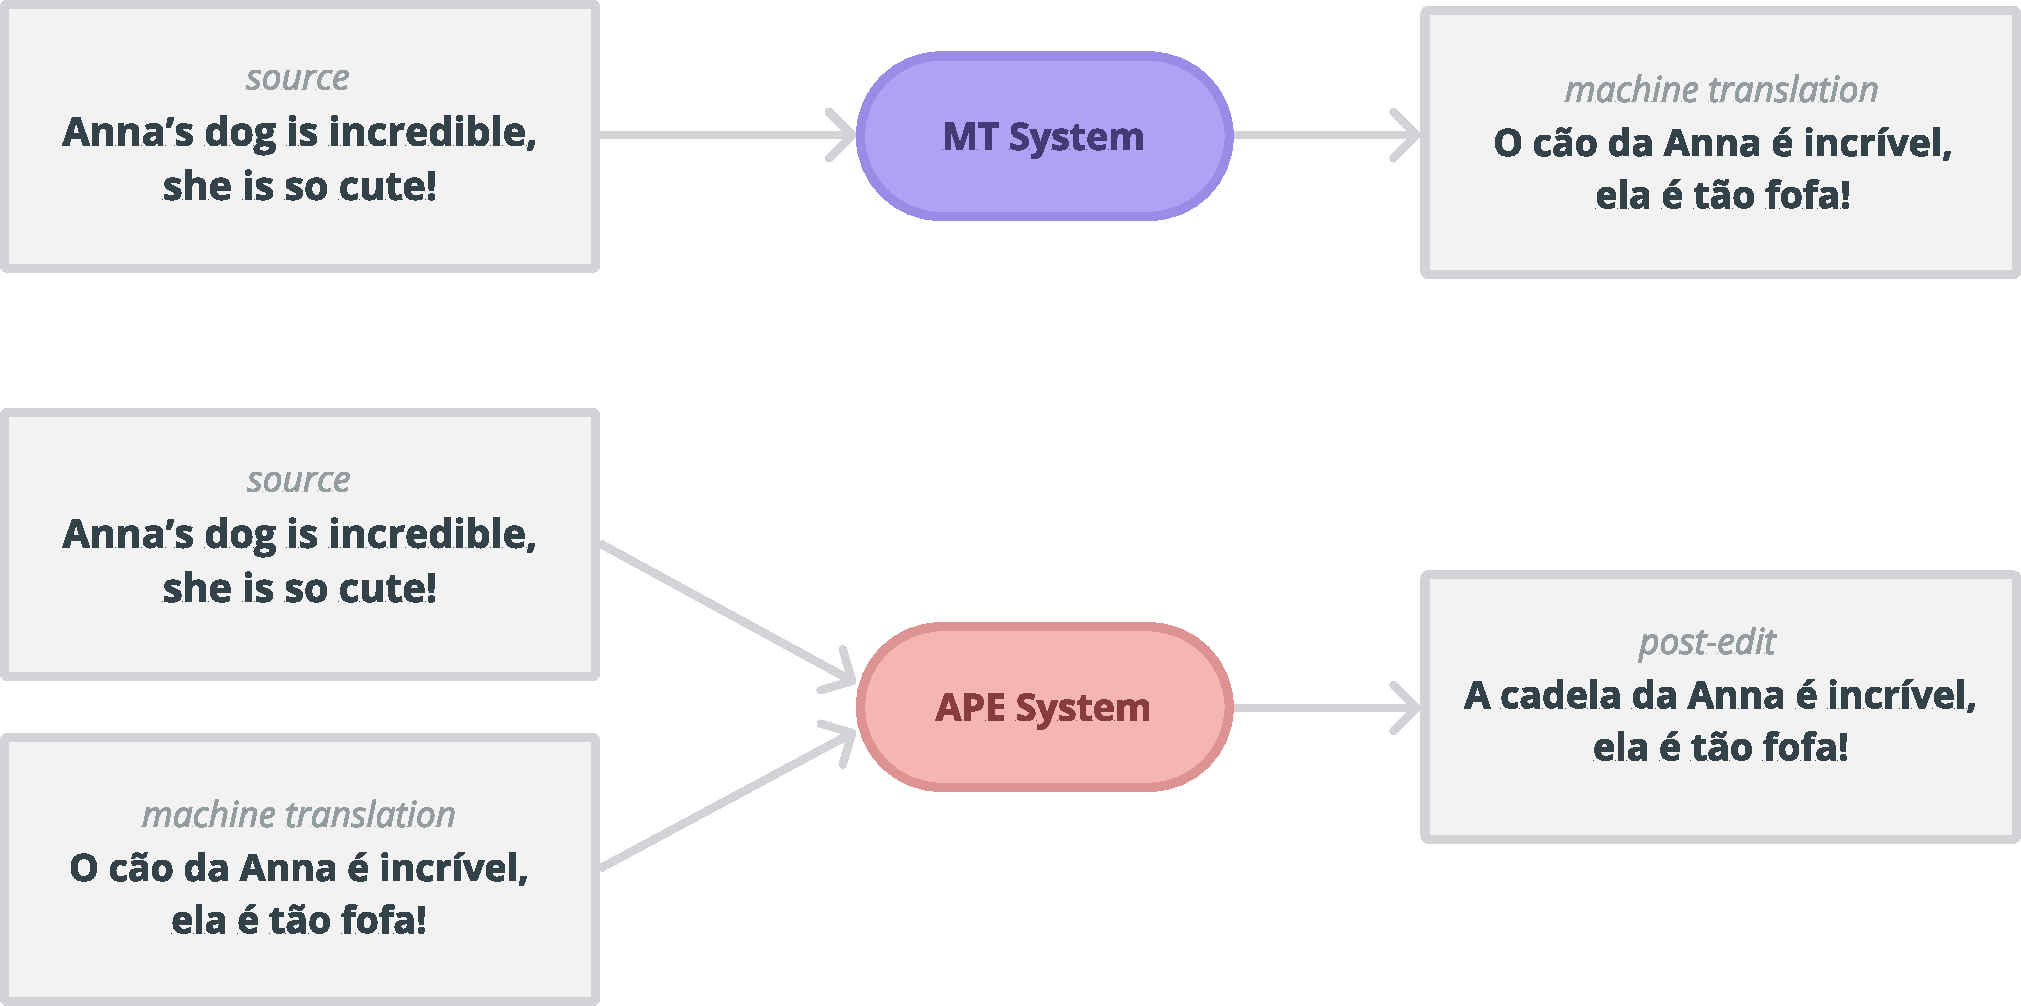
\includegraphics[width=0.5\columnwidth]{figures/ape.pdf}}

%     \begin{itemize}
%         \uncover<3->{\item[] This task is easier than doing MT from scratch}
%         \uncover<4->{\item[] Can we do ``APE'' integrated into the MT pipeline?}
%     \end{itemize}
% \end{frame}

\begin{frame}
    \frametitle{Idea: create a latent, draft translation}
    \centering

    \begin{itemize}
        \uncover<1->{\item[] ... with a memory of phrase alignments}
    \end{itemize}

    \centering
    \uncover<2->{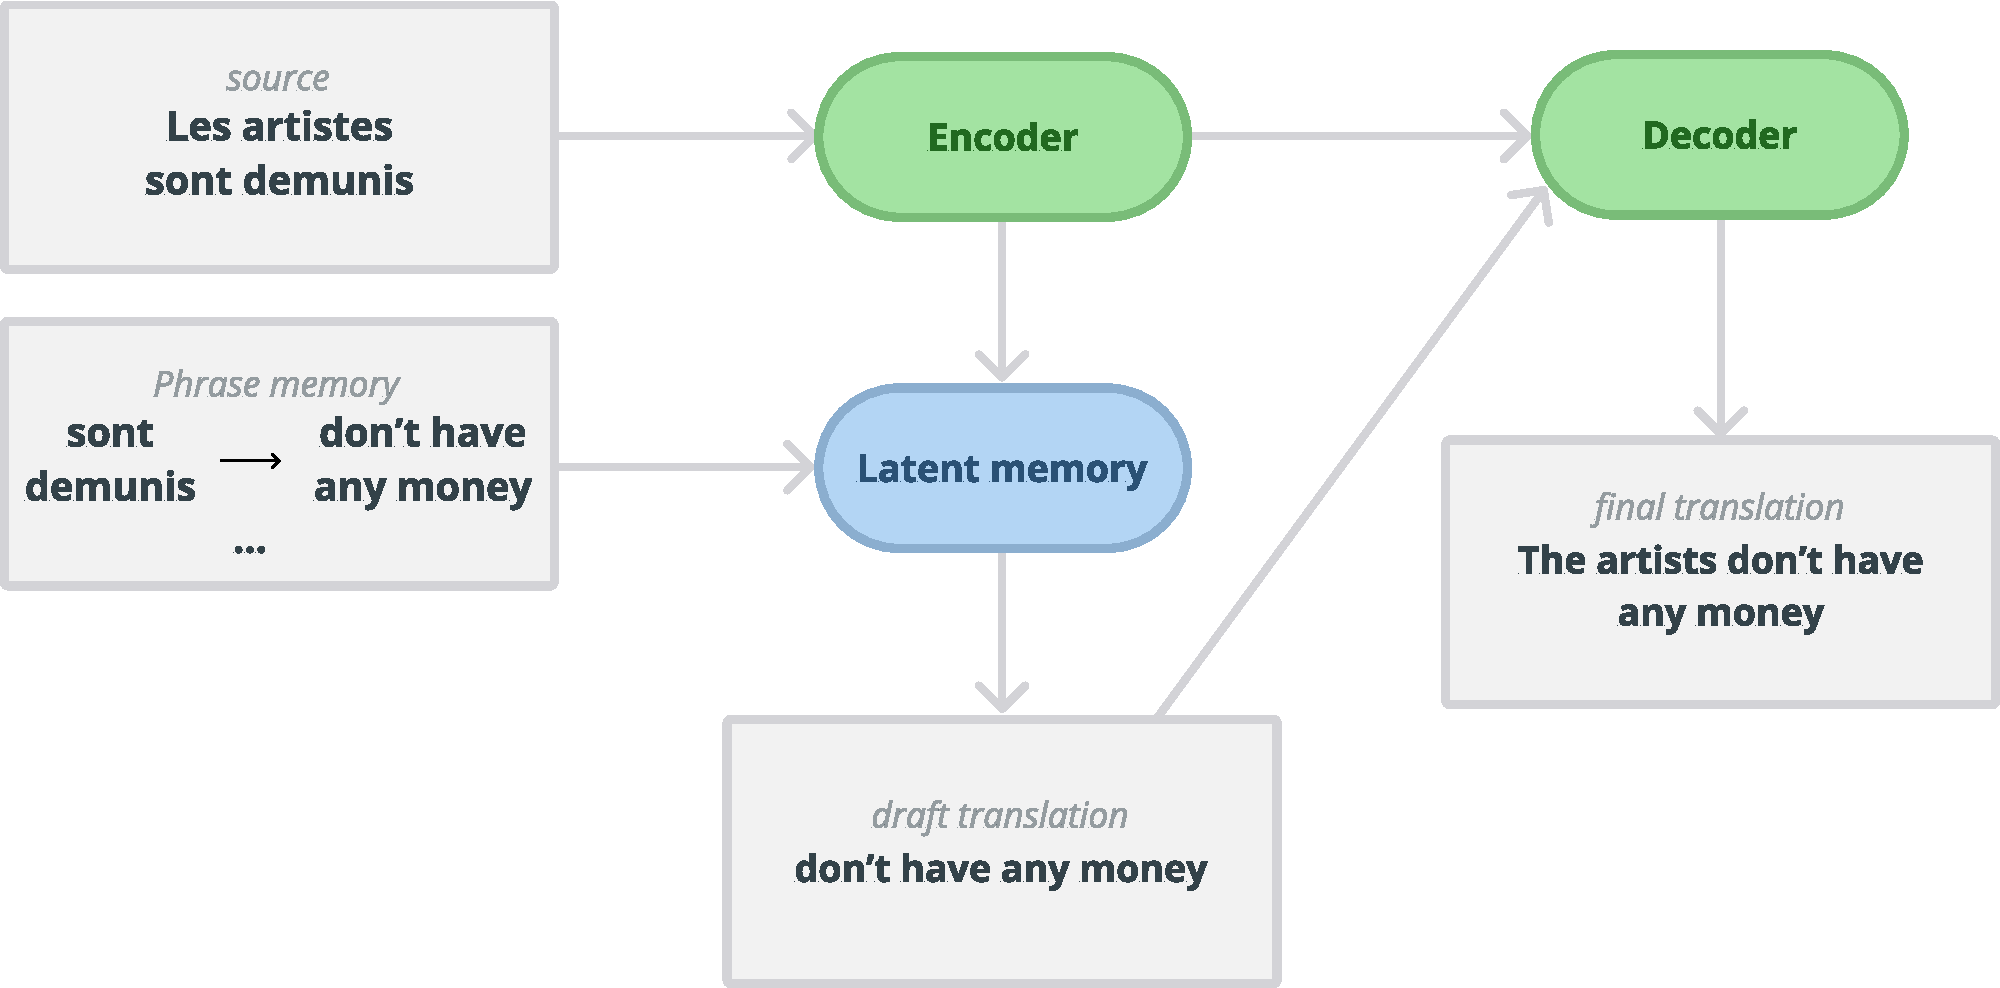
\includegraphics[width=0.8\columnwidth]{figures/nmtdrafts.pdf}}

\end{frame}

% \begin{frame}
%     \frametitle{Translating by editing a draft}
%     \centering
%     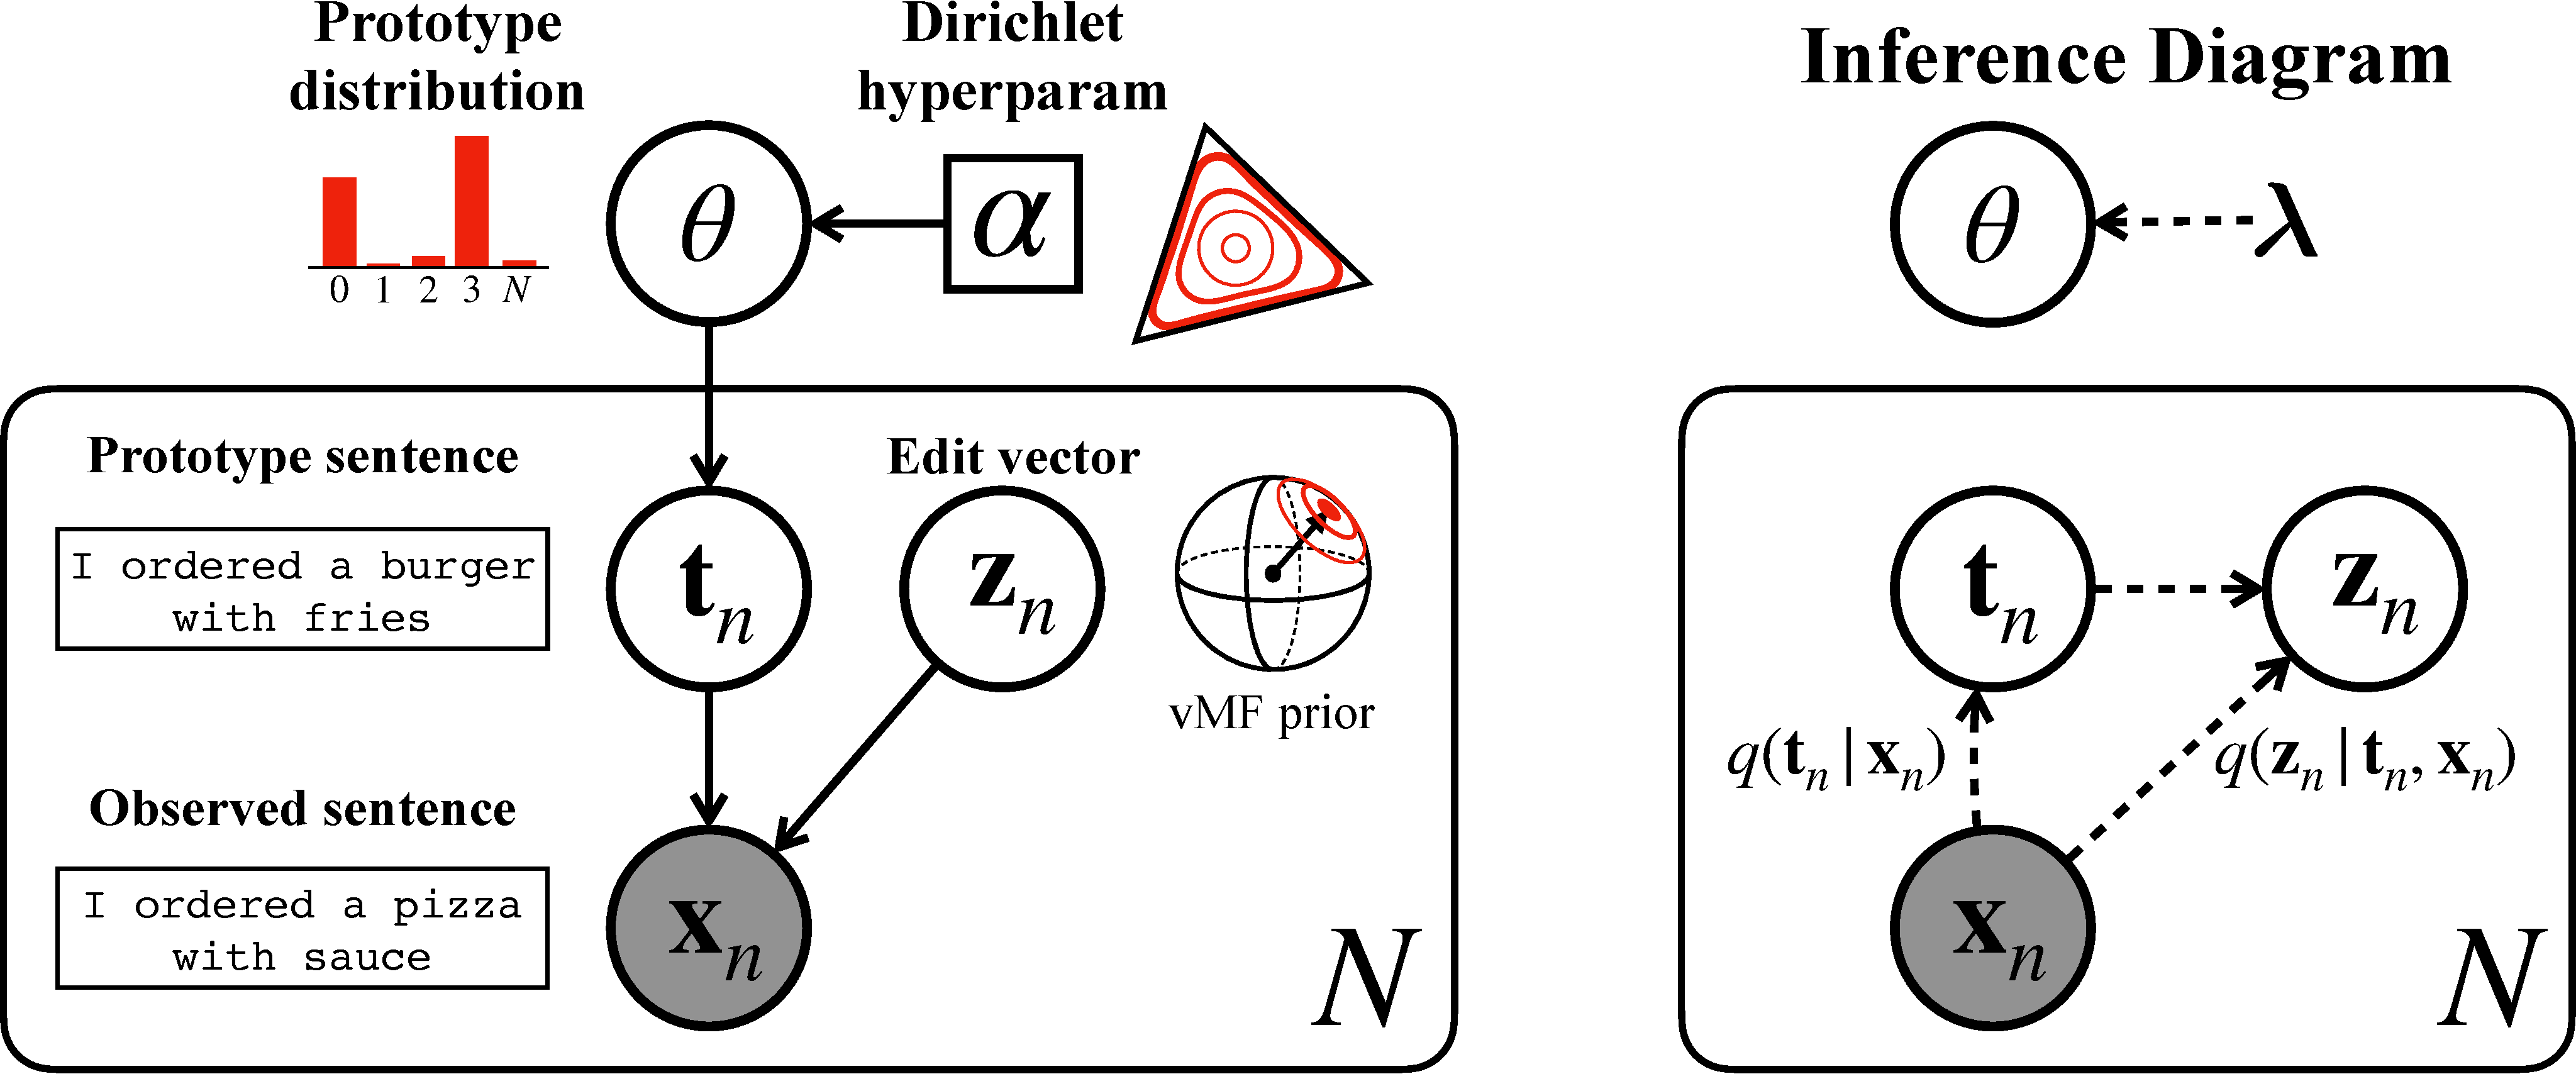
\includegraphics[width=0.8\columnwidth]{figures/heetalmodel.pdf}
% \end{frame}

\begin{frame}
    \frametitle{Translation through transduction}

    \begin{figure}[t]
        \centering
        
        \begin{tikzpicture}
            % Define nodes
            \node[obs]                (y)     {\color{tMidnight} $ y $};
            %\node[semi, left =of y]   (x) {\color{tMidnight} $ x $};
            \node[latent, above =of y] (t) {\color{tMidnight} $ t $};
            \node[latent, left =of t] (z) {\color{tMidnight} $ z $};
            \node[obs,below =of z]   (x) {\color{tMidnight} $ x $};
            
            % Connect nodes
            \edge{x}{z,t};
            \edge{t,z}{y};
            
            \plate{data}{(x)(y)(t)(z)}{$N$};
        \end{tikzpicture}
        ~
        \begin{tikzpicture}
            % Define nodes
            \node[obs]                (y)     {\color{tMidnight} $ y $};
            %\node[semi, left =of y]   (x) {\color{tMidnight} $ x $};
            \node[latent, above =of y] (t) {\color{tMidnight} $ t $};
            \node[latent, left =of t] (z) {\color{tMidnight} $ z $};
            \node[obs,below =of z]   (x) {\color{tMidnight} $ x $};
            
            % Connect nodes
            \edge[dashed]{y}{z};
            \edge[dashed]{y}{t};
            
            \plate{data}{(x)(y)(t)(z)}{$N$};
        \end{tikzpicture}
    \end{figure}
    
\end{frame}

\begin{frame}
    \frametitle{Another Idea: using latent summaries in NMT}

    \centering
    \uncover<2->{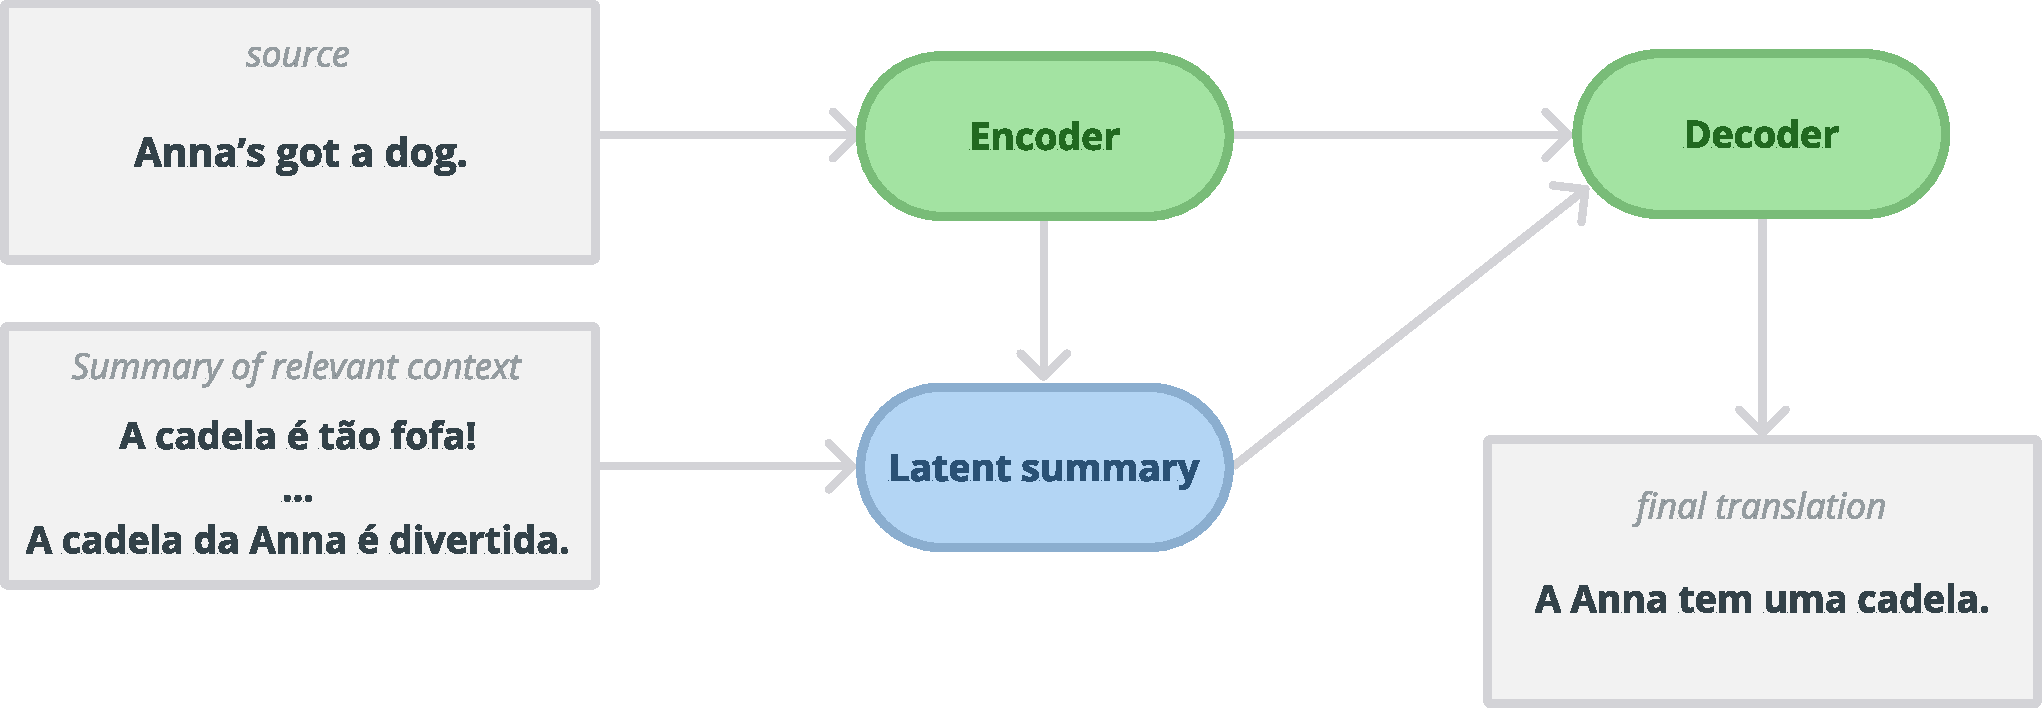
\includegraphics[width=0.8\columnwidth]{figures/summary.pdf}}

\end{frame}

% \begin{frame}
%     \frametitle{Using latent summaries in NMT}

%     \begin{figure}[t]
%         \centering
%         \begin{tikzpicture}
%             % Define nodes
%             \node[obs]                (y)     {\color{tMidnight} $ y $};
%             \node[obs, left =of y]   (xi) {\color{tMidnight} $ X $};
%             \node[latent, above =of xi] (z) {\color{tMidnight} $ z $};
    
%             % Connect nodes
%             \edge{xi,z}{y};
%             \edge{xi}{z};
    
%             \plate{data}{(y)}{$N$};
%         \end{tikzpicture}
%         ~
%         \begin{tikzpicture}
%             % Define nodes
%             \node[obs]                (y)     {\color{tMidnight} $ y $};
%             \node[obs, right =of y]   (xi) {\color{tMidnight} $ X $};
%             \node[latent, above =of xi] (z) {\color{tMidnight} $ z $};
    
%             % Connect nodes
%             \edge[dashed]{xi,y}{z};
            
%             \plate{data}{(y)}{$N$};
%         \end{tikzpicture}
%     \end{figure}
% \end{frame}

\begin{frame}
    \frametitle{Multi-domain NMT}

    \begin{figure}[t]
        \centering
        \begin{tikzpicture}
            % Define nodes
            \node[obs]                (x)     {\color{tMidnight} $ x $};
            \node[obs, below =of x]   (y) {\color{tMidnight} $ y $};
            \node[latent, right =of y] (z) {\color{tMidnight} $ z $};
            \node[latent, above =of x, xshift=1.75cm] (c) {\color{tMidnight} $ c $};
    
            % Connect nodes
            \edge{x,z}{y};
            \edge{c}{z};
            \edge{x}{c};
    
            \plate{data}{(y)(x)(z)}{$N$};
        \end{tikzpicture}
        ~
        \begin{tikzpicture}
            % Define nodes
            \node[obs]                (x)     {\color{tMidnight} $ x $};
            \node[obs, below =of x]   (y) {\color{tMidnight} $ y $};
            \node[latent, right =of y] (z) {\color{tMidnight} $ z $};
            \node[latent, above =of x, xshift=1.75cm] (c) {\color{tMidnight} $ c $};
    
            % Connect nodes
            \edge[dashed]{y}{z};
            \edge[dashed]{x,y}{c};
            
            \plate{data}{(x)(y)(z)}{$N$};
        \end{tikzpicture}
    \end{figure}
\end{frame}

\begin{frame}
    \frametitle{Document-level NMT}

    \begin{figure}[t]
        \centering
        \begin{tikzpicture}
            % Define nodes
            \node[obs]                (y)     {\color{tMidnight} $ y $};
            \node[latent, above =of y] (z) {\color{tMidnight} $ z $};
            \node[latent, left =of z] (c) {\color{tMidnight} $ c $};
            \node[obs, left =of y]   (xi) {\color{tMidnight} $ X $};
    
            % Connect nodes
            \edge{xi,z}{y};
            \edge{c}{z};
            \edge{xi}{c};
    
            \plate{data}{(y)(z)}{$N$};
        \end{tikzpicture}
        ~
        \begin{tikzpicture}
            % Define nodes
            \node[obs]                (y)     {\color{tMidnight} $ y $};
            \node[latent, above =of y] (z) {\color{tMidnight} $ z $};
            \node[latent, right =of z] (c) {\color{tMidnight} $ c $};
            \node[obs, right =of y]   (xi) {\color{tMidnight} $ X $};
            
            % Connect nodes
            \edge[dashed]{y}{z};
            \edge[dashed]{y,xi}{c};
            
            \plate{data}{(y)(z)}{$N$};
        \end{tikzpicture}
    \end{figure}
\end{frame}

\begin{frame}[t,allowframebreaks]
\frametitle{References}
\printbibliography
\end{frame}

\end{document}

